\documentclass[12pt,twoside]{report}
\newcommand\hmmax{0}
\newcommand\bmmax{0}
\usepackage[spanish]{babel}
\usepackage[utf8]{inputenc} %%esto es para las tildes en linux
\usepackage{lipsum}
% \usepackage{mathptmx} si se pone no funciona el \mathcal por alguna razón (?
\usepackage[paper=a4paper, margin=2.5 cm, top=2.5 cm, bottom=2.5cm]{geometry}
\usepackage{comment}
\usepackage{titlesec}
\usepackage{fancyhdr}
\usepackage{amsmath,amssymb,amsthm}
\usepackage{amssymb}
\usepackage{amsthm}
\DeclareMathAlphabet{\mathbbm}{U}{bbm}{m}{n}
\usepackage{marvosym}
\usepackage{comment}
\usepackage[usenames,dvipsnames,svgnames,table]{xcolor}
\usepackage{graphicx}
\usepackage[all]{xy}
\usepackage{ mathrsfs }
\usepackage{nicematrix,tikz}
\usepackage{cancel}
\usepackage{relsize}
\usepackage{amsfonts}
\usepackage{scrextend}
\usepackage{pgfplots}
\usepgfplotslibrary{fillbetween}
\usepackage{hyperref}
\usepackage{tcolorbox}
\usepackage{ wasysym }
\usepackage{wrapfig}
\usepackage[new]{old-arrows}
\usepackage{makeidx}
\usepackage{comment}
\usepackage{arydshln}
\usepackage{units}
\usepackage[new]{old-arrows}
\usepackage{tikz}
\usetikzlibrary{decorations.pathmorphing}
\usepackage{lmodern}
\usepackage{graphicx} % provides "\rotatebox" and "\reflectbox" macros
\usepackage{mathtools}
\usepackage[document]{ragged2e}
\usepackage{ulem}
\usepackage{etoolbox}
\usepackage[shortlabels]{enumitem}
\usepackage{MnSymbol} %\upmapsto \downmapsto
\usepackage{multicol}
\usepackage{tikz-cd}
\usepackage{pgfplots}
\usepgfplotslibrary{fillbetween}
\setlist[enumerate]{nosep}
\makeatletter
\providecommand{\subtitle}[1]{% para poner un \subtitle
  \apptocmd{\@title}{\par {\large #1 \par}}{}{}
}
\makeatother
\newlength{\LETTERheight}
\AtBeginDocument{\settoheight{\LETTERheight}{I}}
\newcommand\rotPi{\rotatebox[origin=c]{180}{$\Pi$}}
\newcommand\longmapsfrom{\rotatebox[origin=c]{180}{$\longmapsto$}}
\newcommand*{\pd}[3][]{\ensuremath{\frac{\partial^{#1} #2}{\partial #3}}}
%%para poner \dfrac{\partial^z x}{\partial y} como \pd[z]{x}{y} 
\newcommand*{\pdd}[3][]{\ensuremath{\dfrac{\partial^{#1} #2}{\partial #3}}}
%%para poner \dfrac{\partial^z x}{\partial y} como \pd[z]{x}{y} 


\pagestyle{fancy}
\fancyhf{}
\fancyhead[LE,RO]{\bfseries \thepage}
\fancyhead[RE,LO]{\itshape \leftmark}
\titleformat{\chapter}[hang]{\bfseries\Large}{Capítulo \thechapter. }{6pt}{}
\titlespacing*{\chapter}{0pt}{0pt}{20pt}
\titleformat{\section}[hang]{\bfseries\large}{\thesection.}{4pt}{}
\titlespacing*{\section}{0pt}{20pt}{10pt}
\titleformat{\subsection}[hang]{\bfseries\normalsize}{\thesubsection.}{6pt}{}
\titleformat{\subsubsection}[hang]{\itshape\normalsize}{\thesubsubsection.}{6pt}{}
\linespread{1.5}
\parskip=10pt
    
\newcommand*{\bint}{\mathlarger{\int}} 
\newcommand*{\bbint}{\mathlarger{\mathlarger{\int}}}    
\newcommand\isom{\xrightarrow{
   \,\smash{\raisebox{-0.65ex}{\ensuremath{\scriptstyle\sim}}}\,}}
\newcommand{\modulo}[2]{{\raisebox{.2em}{$#1$}\left/\raisebox{-.2em}{$#2$}\right.}}
\newcommand{\rad}{\text{Rad}\,}
\newcommand\mc[1]{\mathcal{#1}}

\newtheoremstyle{plain}
{0pt} % Space above
{10pt} % Space below
{} % Body font
{} % Indent amount
{\itshape} % Theorem head font
{.} % Punctuation after theorem head
{.5em} % Space after theorem head
{} % Theorem head spec (can be left empty, meaning `normal')

\newtheoremstyle{azul}
{0pt} % Space above
{10pt} % Space below
{} % Body font
{} % Indent amount
{\bfseries \color{blue}} % Theorem head font
{.} % Punctuation after theorem head
{.5em} % Space after theorem head
{} % Theorem head spec (can be left empty, meaning `normal')

\newtheoremstyle{azul2}
{0pt} % Space above
{10pt} % Space below
{} % Body font
{} % Indent amount
{\itshape \color{blue}} % Theorem head font
{.} % Punctuation after theorem head
{.5em} % Space after theorem head
{} % Theorem head spec (can be left empty, meaning `normal')


\theoremstyle{azul}
  \newtheorem*{propx}{Proposición}
  \newtheorem*{demx}{Demostración}
  \newtheorem*{defix}{Definición}
  \newtheorem*{propix}{Propiedades}
  \newtheorem*{corx}{Corolario}
  \newtheorem*{notax}{Nota}
  \newtheorem*{ejex}{Ejemplos}

\theoremstyle{azul2}
  \newtheorem*{obsx}{Observación}

  
\theoremstyle{definition}
  \newtheorem{eje}{Ejemplo}
  \newtheorem*{ejes}{Ejemplos}
  \newtheorem*{clasi}{Clasificación}
  \newtheorem{defi}{Definición}
  \newtheorem*{defin}{Definición}
  \newtheorem*{propi}{Propiedades}
  \newtheorem*{intgraf}{Interpretación gráfica}
  \newtheorem{demos1}{Demostración}
  \newtheorem*{teo}{Teorema}
  \newtheorem*{cor}{Corolario}
  \newtheorem*{coro}{Corolario}  
  \newtheorem*{ejers}{Ejercicios}
  \newtheorem*{ejer}{Ejercicio}
  \newtheorem*{ejem}{Ejemplo}
  \newtheorem*{ejems}{Ejemplos}
  \newtheorem*{ejern}{Ejercicio}
  \newtheorem*{met}{Método}
  \newtheorem{pro}{Proposición}
  \newtheorem*{prop}{Proposición}
  \newtheorem{prop1}{Proposición}
  \newtheorem*{lem}{Lema}

\theoremstyle{plain}
  \newtheorem*{obs}{Observación}
  \newtheorem*{sol}{Solución}
  \newtheorem*{pag}{Página}  
  \newtheorem*{dem}{Demostración}
  \newtheorem*{nota}{Nota}

\usepackage{afterpage}

\newcommand\blankpage{%
    \null
    \thispagestyle{empty}%
    \addtocounter{page}{-1}%
    \newpage}
  
  
\title{\textit{\textbf{Análisis Numérico I y II}}}
\author{Sara Santos García \;\;\; Pablo Zurrón García}
\subtitle{2º Matemáticas, Universidad de Salamanca}
%\hypersetup{draft}
\begin{document}
\maketitle
\afterpage{\blankpage}
\afterpage{\blankpage}
\tableofcontents
\vfill
\newpage
\addcontentsline{toc}{chapter}{\textbf{ANÁLISIS NUMÉRICO I}} 
\chapter{Aproximaci{\'o}n de ra{\'i}ces}
    \section{Introducción}
    \justifying 
    En este capítulo se desarrollarán métodos numéricos para aproximar las soluciones (reales) de ecuaciones del tipo $f(x)=0$. La motivación de estos métodos es la necesidad de determinar la expresión en base decimal de las soluciones de una ecuación cuando dichas soluciones no son números racionales. 

    La forma de construir la mayoría de métodos será a partir de sucesiones de números racionales que convergerán a la solución de $f(x)=0$ ya que, por definición, todo número real es el límite de una sucesión de Cauchy de números racionales.

    Algo a tener en cuenta a la hora de emplear un método numérico es el error cometido. Como es imposible conocer el valor exacto del error (ya que entonces sabríamos cuál es la solución exacta), lo que haremos será acotar dichos errores. 
    \section{Algoritmo babilónico}
    \begin{ejem}
    
    Considerando la ecuación $x^2-2=0$, las soluciones son $x=\pm \sqrt{2}$, pero queremos saber la solución exacta (en el sentido numérico). Para ello, podemos generar una sucesión que converja a ella y que lo haga lo suficientemente rápido. 

    Consideremos la aproximación $x_o=1,5$, observemos que $\dfrac{2}{x_o}< 2$ y haciendo la media de ellas, obtenemos la siguiente aproximación:
    $$x_1=\dfrac{1}{2}\left(x_o+\dfrac{2}{x_o}\right)=1,4166...$$
    y de la misma forma
    $$x_2=\dfrac{1}{2}\left(x_1+\dfrac{2}{x_1}\right)=1,41421686...$$
    y dado que $\sqrt{2}=1,414213...$, hemos obtenido un error mínimo en unas pocas iteraciones. Veamos ahora el caso general.
    \end{ejem}
    \begin{met}[\textbf{Algoritmo babilónico}]
    Sea $a>0$. Queremos aproximar $\alpha=\sqrt{a}>0$, es decir, la raíz positiva de la ecuación
    $$x^2-a=0$$
    Dado $x_o>\alpha$, definimos la siguiente sucesión de aproximaciones:
    \begin{align}
    x_n=\frac{1}{2}\left(x_{n-1}+\frac{a}{x_{n-1}}\right)\qquad n\geq 1
    \end{align}
    Que convergerá al valor $\alpha$ con error 
    $$\varepsilon_{n}\leq k \cdot \varepsilon_{n-1}^2$$
    \end{met}
    \begin{dem}
    Calculemos en primer lugar el error cometido en la $n-$ésima iteración:
    $$\varepsilon_n=x_n-\alpha=\frac{1}{2}\left(x_{n-1}+\frac{a}{x_{n-1}}\right)-\alpha=\frac{1}{2x_{n-1}}(x_{n-1}^2+a-2\alpha x_{n-1})=\frac{1}{2x_{n-1}}(x_{n-1}-\alpha)^2>0$$
    luego $x_n>\alpha$ y como $\varepsilon_{n-1}=x_{n-1}-\alpha$, se deduce que
    $$\varepsilon_n=\frac{1}{2x_{n-1}}\cdot \varepsilon_{n-1}^2\leq \frac{1}{2\alpha}\cdot \varepsilon_{n-1}^2=k\cdot \varepsilon_{n-1}^2$$
    Veamos la convergencia del método:
    $$x_{n+1}-x_n=\frac{1}{2}\left(x_n+\frac{a}{x_n}\right)-x_n=\frac{1}{2x_n} \: a-\frac{1}{2} \: x_n=\frac{1}{2x_n}(a-x_n^2)=\frac{1}{2x_n}(\alpha-x_n)(\alpha+x_n)<0$$
    Como la sucesión es decreciente y acotada ($x_n>\alpha$) sabemos que converge. Tomando límites en $(1)$ y denotando por $\ell$ a dicho límite, obtenemos la siguiente ecuación:
    $$\ell=\frac{1}{2}\left(\ell+\frac{a}{\ell}\right)\Longrightarrow 2\ell^2=\ell^2+a\Longrightarrow \ell=\sqrt{a}=\alpha$$
    \qed\end{dem} 
    \begin{obs}
    El hecho de que el error en la iteración $n-$ésima esté acotado por el error de la iteración anterior al cuadrado indica que en cada aproximación el número de decimales que coinciden con el valor real se duplica. Esto se puede observar en el primer ejemplo.
    \end{obs}
    \section{{\'O}rdenes de convergencia} 
    \begin{defin}
        Sea $\{x_n\}$ una sucesión convergente con límite $L$, diremos que $\{x_n\}$  tiene un \textbf{orden de convergencia lineal} si 
        $$|x_{n+1}-L|\leq k \cdot |x_n-L| \qquad k <1$$
        Diremos que la sucesión $\{x_n\}$ tiene un \textbf{orden de convergencia cuadrática} si 
        $$|x_{n+1}-L|\leq k \cdot |x_n-L|^2 $$
        En general, diremos que la convergencia de $\{x_n\}$ es de \textbf{orden }$\mathbf{a}$ si
        $$|x_{n+1}-L|\leq k \cdot |x_n-L|^a $$
        El caso $1<a<2$ se denomina convergencia \textbf{superlineal}.
    \end{defin}

    \begin{obs}
    Equivalentemente, podemos definir los ordenes de convergencia como sigue.  Sea $\{x_n\}$ una sucesión convergente con límite $L$, diremos que la convergencia es lineal o de orden 1 cuando
        $$\lim_{n \to \infty} \dfrac{|x_{n+1}-L|}{|x_n-L|}=k < 1$$
        En general, la convergencia es de orden $a>1$ cuando 
        $$0 < \lim_{n \to \infty} \dfrac{|x_{n+1}-L|}{|x_n-L|^a}=k < +\infty$$

    \end{obs}
    
\section{M{\'e}todo de la bisecci{\'o}n}
        
       \begin{prop}
        Sea $f: \mathbb{R} \longrightarrow \mathbb{R}$ una función real de variable real. Si $f$ es continua en $I \subset \mathbb{R}$ y $f(a) \cdot f(b) < 0$ para $a < b \in I$ entonces existe $\alpha \in (a,b)$ tal que $f(\alpha)=0$. Además, si $f$ es derivable en $I$ y $f'(x) \neq 0 \: \forall x \in (a,b)$, entonces $\alpha$ es única.           
           \end{prop}
\begin{dem}
Como $f$ es continua en $[a,b]$, aplicando el teorema de Bolzano sabemos que existe $\alpha\in(a,b)$ tal que $f(\alpha)=0$. Por el teorema de Rolle, si existieran $\alpha_1,\alpha_2$ tales que $f(\alpha_1)=f(\alpha_2)=0$ existiría un punto $c\in (\alpha_1,\alpha_2)\subset(a,b)$ tal que $f'(c)=0$, lo cual contradice lo supuesto.
\qed\end{dem}
\begin{met}[\textbf{de la bisección}]
Sea $a<b$, $x_o=a$,  $y_o=b$ y $z_o=\frac{1}{2}(x_o+y_o)$. Queremos aproximar la solución de la ecuación $f(x)=0$. Si $f(a)\cdot f(b)<0$, por la proposición anterior sabemos que existe $\alpha\in(a,b)$ tal que $f(\alpha)=0$. Con lo cual: \vspace{-5mm}
\begin{itemize}
\item Si $f(z_o)=0$, entonces $\alpha=z_o$ es la solución.
\item Si $f(z_o) \neq 0$, tenemos dos opciones,
\begin{itemize}
    \item Si $f(x_o) \cdot f(z_o) < 0$, entonces tomamos $x_1=x_o, \: y_1=z_o,\: z_1=\frac{1}{2}(x_1+y_1)$
    \item Si $f(x_o) \cdot f(z_o)>0$, entonces tomamos $x_1=z_o, \: y_1=y_o,\: z_1=\frac{1}{2}(x_1+y_1)$
\end{itemize}
\end{itemize}
Aplicando la proposición anterior en $(x_1,y_1)$ nos aseguramos de que $\alpha\in(x_1,y_1)$. Reiterando este proceso, construimos tres sucesiones $\{x_n\}, \: \{z_n\}, \: \{y_n\}$ tales que $x_n\leq z_n\leq y_n$. Observemos además que
\begin{enumerate}[a)]
    \item $\{x_n\}$ es una sucesión creciente y acotada (superiormente) por $\{y_n\}$ 
    
    \item $\{y_n\}$ es una sucesión decreciente y acotada (inferiormente) por $\{x_n\}$

Luego ambas sucesiones son convergentes. Denotemos por $\alpha,\beta$ a los límites de $\{x_n\}$ e $\{y_n\}$ respectivamente. Se tiene entonces que:
$$\beta-\alpha=\underset{n\to\infty}{\lim}(y_n-x_n)=\underset{n\to\infty}{\lim}\frac{b-a}{2^n}=0$$
\item  Como $f$ es continua, $\{f(x_n)\}$ es una sucesión convergente (análogamente $f(\{y_n\})$). Además,  \vspace{-3mm}
$$f(x_n) \cdot f(y_n) <0 \: \Rightarrow \:  \lim_{n \to \infty} f(x_n) \cdot f(y_n) \leq 0 \: \Rightarrow \: \lim_{n \to \infty} f(x_n)  \lim_{n \to \infty} f(y_n) =f(\alpha)^2\leq 0$$
por tanto, $f(\alpha)=0.$
\end{enumerate}
Estudiemos ahora el error del método. Sea $\{z_n\}$ la sucesión que obtenemos por el método de la bisección, y sea 
$$\varepsilon_n=z_n - \alpha$$
el error en el término $n$, entonces, por lo visto en b),
$$|\: \varepsilon_n|=|z_n - \alpha|< \dfrac{b-a}{2^{n+1}}$$
De esta manera, si queremos aproximar $\alpha$ con un error (en valor absoluto) menor que $\varepsilon$, tendrá que ser 
$$|\varepsilon_n|=\dfrac{b-a}{2^{n+1}} < \varepsilon \iff 2^{n+1} > \dfrac{b-a}{\varepsilon} \iff (n+1) \log(2) > \log(b-a) - \log(\varepsilon) $$
Es decir, $$n > \dfrac{\log(b-a)-\log(\varepsilon)}{\log(2)}-1$$
para el $\varepsilon$ que se quiera elegir.
\end{met}
\begin{intgraf} Podemos ver un ejemplo de este método con la siguiente figura, donde escogemos $\alpha \in [a,b]$ ya que $\alpha\approx 1.41$ y $[a,b]=[0'7,1'8]$, y hacemos un par de iteraciones, observando como acotamos la raíz, pero la convergencia no es óptima.
$$\begin{tikzpicture}[scale=3, domain=-1:2, samples=70,  trig format=rad]
    
	% draw axis
	\draw[->] (-0.3,0) -- (3,0) node[below right] {$x$};
	\draw[->] (0,-0.5) -- (0,1.3) node[above left] {$y$};
	
	% draw function
	\draw[blue, thick] plot[domain=0.2:2.2] (\x,0.33*\x*\x-0.5) node[above right] {\footnotesize $f(x)=x^2-4$};

    \draw[fill=black] (1.23,0) circle [radius=0.01] node[above] {$\alpha$};
     \draw[fill=black] (0.7,0) circle [radius=0.01] node[above] {$a=x_o=x_1$ \hspace{15mm}};
     \draw[fill=black] (2,0) circle [radius=0.01] node[below right] {$b=y_o$ \; \; };
     \draw[dotted] (2,0) -- (2,0.82);
     \draw[dotted] (0.7,0) -- (0.7,-0.34);
     \draw[fill=black] (1.35,0) circle [radius=0.01] node[below right] {$z_o=y_1\; \; \; \;$};
     \draw[<-] (1.025,-0.01) -- (1.2,-0.3)  node[below] {$\; \; \; z_1$};
     \draw[->] (1.025,0) circle [radius=0.01];
     
\end{tikzpicture}$$    
\end{intgraf}
\begin{ejem}
    Escogiendo $\varepsilon=10^{-8}$, para hallar $\sqrt{2}$ y eligiendo $a=1, \: b=2$, $$n>\dfrac{\log(1)-\log(10^{-8})}{\log(2)}=\dfrac{8\log(10)}{\log(2)} = 8 \cdot \log_2(10) > 26$$
    Es decir, hacemos más de 26 iteraciones, que comparadas con las 3-4 que necesitábamos con el método babilónico, nos da un método mucho más lento.
\end{ejem}
\begin{obs}\:\vspace{-5mm}
    \begin{enumerate}[a)]
        \item No se calcula el producto $f(x_n)\cdot f(z_n)$, solo se mira el signo de $f(z_n)$
        \item No se calcula $z_o=\dfrac{1}{2}(x_o+y_o)$, sino 
        $$z_o=x_o+\dfrac{\Delta_o}{2} \quad \Delta_o=y_o-x_o$$
        teniendo así en $\Delta_i$ el error de la iteración $i$.
    \end{enumerate}
\end{obs}
    \section{M{\'e}todo del punto fijo}
       \begin{defin}
           Un \textbf{punto fijo} de una aplicación
           $g$ es aquel tal que $$g(\alpha)=\alpha$$
           En el caso de funciones $g: \mathbb{R} \longrightarrow \mathbb{R}$, se trata de encontrar la solución de la ecuación $g(x)=x$.
       \end{defin}
       \begin{teo}[\textbf{del punto fijo de Brower}] Si $f: [a,b] \longrightarrow [a,b]$ con $a,b \in \mathbb{R}$ es continua, entonces $f$ tiene un punto fijo, $\alpha\in[a,b]$.
       \end{teo}
       \begin{dem}
           El caso $f(a)=a$ ó $f(b)=b$ es trivial. Si $f(a)\neq a$, entonces $f(a)>a$, luego $f(a)-a>0$, y de la misma forma, $f(b)-b <0$. Como la función $g(x)=f(x)-x$ es continua, por el Teorema de Bolzano, existe $\alpha \in (a,b)$ tal que $$0=g(\alpha)=f(\alpha)-\alpha \: \iff \: f(\alpha)=\alpha$$ 
       \qed\end{dem}
       \begin{defin}
           Una función $f$ se dice que es \textbf{contractiva} cuando existe una constante $k < 1$ tal que
           $$|f(x)-f(y)| \leq k \cdot |x-y|$$
       \end{defin}
       \begin{defin}
       Las funciones que verifican $$|f(x)-f(y)|\leq L \cdot |x-y|$$ para cierta $L \in \mathbb{R}$ se llaman \textbf{funciones lipschitzianas}.
       \end{defin}
       \begin{teo} [\textbf{del punto fijo de Banach}] Si $f: [a,b] \longrightarrow [a,b]$ es contractiva, entonces $f$ tiene un único punto fijo. 
       \end{teo}
       \begin{dem}
           Por ser $f$ contractiva, es continua y aplicando el Teorema del Punto Fijo de Brower, tiene un punto fijo. Veamos que el punto fijo es único. Supongamos que existen dos distintos, $\alpha, \beta$, entonces sería
           $$|\alpha-\beta|=|f(\alpha)-f(\beta)| \leq k \cdot |\alpha-\beta| < \alpha-\beta$$
           lo cual es una contradicción, luego existe un único punto fijo.
       \qed\end{dem}
       \begin{ejer}
       Si $f: \mathbb{R} \longrightarrow \mathbb{R}$ es contractiva, entonces $f$ tiene un único punto fijo.
       \end{ejer}
       \begin{met}[\textbf{del punto fijo}] Si $f$ es una aplicación contractiva en un entorno $I$ de un punto fijo $\alpha$, entonces para todo $x_o \in I$, la sucesión
       \begin{align}
           x_{n+1}=f(x_n) \qquad n \geq 0
           \label{met:punto}
        \end{align}
           converge a $\alpha$ con un orden de convergencia lineal:
           $$|\varepsilon_n|\leq k |\varepsilon_{n-1}| \qquad k<1$$
       \end{met}
       \begin{dem}
       Veamos en primer lugar que la sucesión converge a $\alpha$:
           $$|x_{n+1}- \alpha|=|f(x_{n})-f(\alpha)|\leq k \cdot |x_n - \alpha|\leq k^2 \cdot |x_{n-1}- \alpha| \leq \cdots \leq k^{n+1} \cdot |x_o - \alpha|$$
Como $\underset{n \to \infty}{\lim} k^n=0$, dado $\varepsilon>0$ existe $n_o \in \mathbb{N}$ tal que para todo $n > n_o$, $k^{n+1} < \frac{\varepsilon}{|x_o-\alpha|}$, de forma que para todo $n>n_o$ se verifica que
$$|x_{n+1}-\alpha|<k^{n+1}\cdot |x_o-\alpha|<\frac{\varepsilon}{|x_o-\alpha|}\cdot |x_o-\alpha| <\varepsilon$$
Estudiemos ahora el error. El error cometido en la $n$-ésima iteración será $|\varepsilon_n|=|x_n-\alpha|$ y por ser $f$ contractiva se tiene que
$$|\varepsilon_{n}|=|x_{n}-\alpha|=|f(x_{n-1})-f(\alpha)|\leq k \cdot |x_{n-1} - \alpha| = k \cdot |\varepsilon_{n-1}|$$
            Es decir, el método del punto fijo tiene un orden de convergencia lineal.
       \qed\end{dem} 
       \begin{intgraf} Podemos ver a continuación un ejemplo del método, donde observamos como nos vamos enroscando sobre el punto fijo $\alpha$ de $\cos(x)$, que como se puede observar debajo, es la solución o raíz de $\cos(x)-x$, que hemos llamado $\beta$.
$$\begin{tikzpicture}[scale=5, domain=-1:2, samples=70,  trig format=rad]
	
	% draw axis
	\draw[->] (-0.3,0) -- (2,0) node[below right] {$x$};
	\draw[->] (0,-0.5) -- (0,1.3) node[above left] {$y$};
	
	% draw function
	\draw[blue, thick] plot[domain=-0.1:2] (\x,{cos(\x)}) node[above right] {\footnotesize $f(x)=\cos(x)$};
    \draw[blue, thick] plot[domain=-0.1:1.2] (\x,{(\x)}) node[right] {\footnotesize $f(x)=x$};
    \draw[black, thick] plot[domain=-0.1:1] (\x,{cos(\x)-\x}) node[right] {\footnotesize $f(x)=\cos(x)-x$};

    \draw[fill=black] (0.74,0.74) circle [radius=0.01] node[above] {$\alpha$};
    \draw[fill=black] (0.74,0) circle [radius=0.01] node[below] {$\beta$};
    \draw[dotted] (0.74,0.74) -- (0.74,0);
    \def\x{1}
    \draw[fill=black] (\x,0) circle [radius=0.01] node[below] {$x_o$};
    \draw[dotted] (\x,0) -- (\x,{cos(\x)});
    \def\y{0.54}
    \draw[fill=black] (\y,0) circle [radius=0.01] node[below] {$x_1$};
    \draw[dotted] (\y,0) -- (\y,\y);
    \draw[red,fill=red] (\x,{cos(\x)}) circle [radius=0.01];
    \draw[->,red](\x,{cos(\x)}) -- (\y,\y) ;
    \draw[dotted] (\y,0) -- (\y,{cos(\y)}); 
    \draw[->,red](\y,\y) -- (\y,{cos(\y)});

    \def\z{0.86}
    \draw[fill=black](\z,0) circle [radius=0.01] node[below] {$x_2$};
    \draw[dotted] (\z,0) -- (\z,\z);
    \draw[->,red] (\y,{cos(\y)}) -- (\z,\z);
    \draw[red,->] (\z,\z) -- (\z,{cos(\z)});

    \def\t{0.65}
    \draw[fill=black](\t,0) circle [radius=0.01] node[below] {$x_3$};
    \draw[dotted] (\t,0) -- (\t,\t);
    \draw[->,red] (\z,{cos(\z)}) -- (\t,\t);
    \draw[red,->] (\t,\t) -- (\t,{cos(\t)});

    
\end{tikzpicture}$$
       \end{intgraf}
       \begin{ejem}
           El algoritmo babilónico
           $$x_{n+1}=\dfrac{1}{2}\left( x_n + \dfrac{a}{x_n}\right)$$
           aproxima el punto fijo de $g(x)=\frac{1}{2}\left( x + \frac{a}{x}\right)$, es decir, solución de $g(x)=x$ $$x=\frac{1}{2}\left( x + \frac{a}{x}\right) \iff 2x=x+\dfrac{a}{x} \iff x = \dfrac{a}{x} \iff x^2=a$$
           Veamos que $g$ es contractiva en un entorno de $\alpha=\sqrt{a}$. Dado que la contractividad asegura que $$\dfrac{|g(x)-g(y)|}{|x-y|}\leq k <1$$
           Si $g$ es drivable (que lo es en nuestro ejemplo), aplicando el teorema del valor medio tenemos que 
           $$\dfrac{|g(x)-g(y)|}{|x-y|}=|g'(\xi)| \qquad \xi \in (x,y)$$
           Por tanto, si $g'$ es continua en un entorno de $\alpha$ y $|g'(\alpha)|<1$, entonces $|g'(x)|\leq k <1$ en un entorno de $\alpha$. En nuestro caso, $g'(x)=\frac{1}{2}\left(1-\frac{a}{x^2}\right)$, es decir, $g'(\alpha)=g'(\sqrt{a})=0$, luego $|g'(x)|\leq k < 1$
       \end{ejem}
    
    \section{M{\'e}todo de Newton}          
    \begin{teo}[\textbf{de Taylor}]
    Dada $f \in \mc{C}^{n+1}$, se verifica que
    $$f(b)=\sum_{k=0}^n \dfrac{f^{(k)}(a)}{k!}(b-a)^k + R_k(a)$$
    Donde el resto $R_k(a)$ toma las formas de Lagrange e integral
    $$R_k(a)=\dfrac{f^{n+1}(\xi)}{(n+1)!}(b-a)^{n+1} = \dfrac{1}{n!} \int_0^1 f(x) (b-x)^n dx$$
    \end{teo}
    \begin{obs}
        Sea $f: \mathbb{R} \longrightarrow \mathbb{R}$ una función derivable con $f(\alpha)=0$. Una primera aproximación a $\alpha$ es la siguiente:
 
        Dado $x_o$, aproximamos la curva $y=f(x)$ por la tangente en $x=x_o$. La ecuación de la recta tangente es $y=f(x_o)+f'(x_o)(x-x_o)$ de manera que el corte con $y=0$ es:
        $$x_1=x_o-\dfrac{f(x_o)}{f'(x_o)}$$
    \end{obs}
    \begin{met}[\textbf{de Newton}]
        Sea $f$ una función de clase $\mc{C}^2(I)$ con $I \subset \mathbb R$ y sea $\alpha \in I$ tal que $f(\alpha)=0, \: f'(\alpha)\neq 0$. Entonces la sucesión $\{x_n\}$ definida por 
        \begin{align}
          x_{n+1}=x_n-\dfrac{f(x_n)}{f'(x_n)} \qquad n \geq 0
          \label{met:newton}
        \end{align}
        
        coverge a $\alpha$ para $x_o \in I$ suficientemente próximo a $\alpha$. Ademas, dicha convergencia será cuadrática:
        $$|x_{n+1}-\alpha|< C \: |x_n-\alpha|^2 \qquad C=\dfrac{\max|f''(x)|}{2\min|f'(x)|} $$
    \end{met}
    \begin{dem}
        Considerando la función $g(x)=x-\frac{f(x)}{f'(x)}$, observemos que $$g(\alpha)=\alpha-\dfrac{\cancelto{0}{f(\alpha)}}{f'(\alpha)}=\alpha$$es decir, $\alpha$ es un punto fijo de $g$. Si $g$ es contractiva en un entorno de $\alpha$, concluiríamos por la convergencia del punto fijo.

        Calculamos entonces que
        $$g'(x)=1- \dfrac{f'(x)}{f'(x)}+f(x) \: \dfrac{f''(x)}{f'(x)^2}=f(x)\dfrac{f''(x)}{f'(x)^2}$$
        por lo que $$g'(\alpha)=f(\alpha) \: \dfrac{f''(\alpha)}{f'(\alpha)^2}=0$$
        
        Como $g'$ es continua en $\alpha$, dado cualquier $\varepsilon > 0$, podemos encontrar $\delta > 0$ tal que si $|x-\alpha| < \delta$, $$|g'(x)-g'(\alpha)|< \varepsilon \iff |g'(x)|< \varepsilon$$

        Es decir, dado $0 < k < 1$, tomando $\varepsilon=k$ podemos encontrar un $\delta > 0$ tal que si $x \in (\alpha- \delta, \alpha+\delta)$, entonces $|g'(x)| < k$. Dados $x_1,x_2\in(\alpha-\delta,\alpha+\delta)$, por el teorema del valor medio se tiene que
        $$\dfrac{|g(x_1)-g(x_2)|}{|x_1-x_2|}=|g'(\xi)|<k\Rightarrow |g(x_1)-g(x_2)|<k\cdot |x_1-x_2|$$
        y, por tanto, $g$ es contractiva en $(\alpha- \delta, \alpha+\delta)$.
        
        Estudiemos ahora el error del método:
    $$x_{n+1}-\alpha=x_n-\dfrac{f(x_n)}{f'(x_n)} - \alpha=\dfrac{1}{f'(x_n)}(f'(x_n)(x_n-\alpha)-f(x_n))$$
    De la fórmula de Taylor de primer orden se tiene que
    $$0=f(\alpha)=f(x_n)+f'(x_n)(\alpha-x_n)+\dfrac{1}{2}f''(\xi)(\alpha-x_n)^2=f(x_n)-f'(x_n)(x_n-\alpha)+\dfrac{1}{2}f''(\xi)(x_n-\alpha)^2$$
    Por tanto, se tiene que 
    $$x_{n+1}-\alpha=\dfrac{1}{f'(x_n)}f''(\xi)(x_n-\alpha)^2$$
    De esta manera, $$|x_{n+1}-\alpha|=\dfrac{|f''(\xi)|}{2|f'(x_n)|}\: |x_n-\alpha|^2 < \dfrac{\max|f''(x)|}{2\min|f'(x)|}\: |x_n-\alpha|^2 \qquad x \in I$$
    Es decir,
    $$|x_{n+1}-\alpha|< C \: |x_n-\alpha|^2 \qquad C=\dfrac{\max|f''(x)|}{2\min|f'(x)|} $$
    Obteniendo así una convergencia cuadrática.
    \qed\end{dem}
    \begin{intgraf} Véanse las siguientes figuras, una de la $n$-ésima iteración del método de Newton, escogiendo como $x_{n+1}$ el corte de la tangente que pasa por $f(x_n)$, y un ejemplo en el que el método no converge:
    $$\begin{tikzpicture}[scale=2.5, domain=0.3:2, samples=50]
	
	% draw axis
	\draw[->] (-0.1,0) -- (2.5,0) node[below right] {$x$};
	\draw[->] (0,-0.5) -- (0,2.2) node[above left] {$y$};
	
	% draw function
	\draw[blue, thick] plot (\x, {0.5*\x*\x-0.2}) node[left] {\footnotesize $f(x)$};

	% draw x-axis intercept
    \def\x{1.6};
	\draw[dotted] (\x, 0) node[below] {\footnotesize $x_n$} -- (\x,{0.5*\x*\x-0.2});
    \draw[color=red]    plot (\x,1.543*\x-1.4);
    \draw[fill=black] (\x,{0.5*\x*\x-0.2}) circle [radius=0.018] node[left] {\footnotesize $f(x_n)$};
    \draw[fill=black] (\x,0) circle [radius=0.018];
    \draw[fill=black] (0.632,0) circle [radius=0.018] node[below] {\footnotesize $\alpha$};
 
    \def\x{0.9};
	\draw[dotted] (\x, 0) node[below right] {\footnotesize $x_{n+1}$} -- (\x,0.205);
	\draw[fill=black] (\x,0) circle [radius=0.018];
	
\end{tikzpicture}$$
\begin{center}
    Un ejemplo gráfico del Método de Newton en la función $y=\frac{1}{2} \: x^2-\nicefrac{1}{5}$
\end{center}
$$\begin{tikzpicture}[scale=1.5, domain=-1:1.4, trig format=rad, samples=100]
	% draw axis
	\draw[->] (-4,0) -- (4,0) node[right] {$x$};
    \draw[dashed] (-4,1.54) -- (4,1.54) node[right] {\footnotesize $\dfrac{\pi}{2}$};
    \draw[dashed] (-4,-1.54) -- (4,-1.54) node[right] {\footnotesize $-\dfrac{\pi}{2}$};
	% draw function
    \draw[blue,thick] plot[variable=\t,domain=-3:3.3] (\t,{atan(5*\t)}) node[below right] {\footnotesize $f(x)$};
	% draw x-axis intercept
    \def\x{0.4};
    \draw[dotted] (\x, 0) node[below] {\footnotesize $x_o$} -- (\x,{atan(5*\x)});
    \draw[fill=black] (\x,{atan(5*\x)}) circle [radius=0.03];
    \draw[fill=black] (\x,0) circle [radius=0.03];

    \draw[fill=black] (0,0) circle [radius=0.03] node[above left] {\footnotesize $\alpha$};
    \def\x{3};
	\draw[dotted] (\x, 0) node[below right] {\footnotesize $x_2$} -- (\x,{atan(5*\x)});
    \draw[fill=black] (\x,{atan(5*\x)}) circle [radius=0.03];
    \draw[<-,color=red,thick]  (-0.8,0) -- (0.4,{atan(5*0.4)})  ;
    \draw[fill=black] (\x,0) circle [radius=0.03];
    
    \def\x{-0.8};
	\draw[dotted] (\x, 0) node[above left] {\footnotesize $x_1$} -- (\x,{atan(5*\x)});
    \draw[->,color=red,thick] (\x,{atan(5*(\x))}) -- (3,0) ;
    \draw[fill=black] (\x,0) circle [radius=0.03];
    \draw[fill=black] (-0.8,{atan(5*(-0.8))}) circle [radius=0.03];
	\draw[->,color=red,thick] (3,1.525) -- (-3,1.525) ;
\end{tikzpicture}$$
\begin{center}
    Un ejemplo del Método de Newton en el que no converge en la función $y=\arctan(x)$.
\end{center}
    \end{intgraf}
    \begin{ejem}
        Consideremos $f(x)=x^2-a$. Dado $x_o$, el método de Newton para esta ecuación es
        $$x_{n+1}=x_n-\dfrac{f(x_n)}{f'(x_n)}=x_n-\dfrac{x_n^2-a}{2x_n}=\dfrac{2x_n^2-x_n^2+a}{2x_n}=\dfrac{x_n^2+a}{2x_n}=\dfrac{1}{2}\left(x_n+\dfrac{a}{x_n}\right)$$
        Es decir, el método babilónico es el método de Newton aplicado a dicha $f(x)$.
    \end{ejem}
    \begin{ejem}
        Considerando ahora $f(x)=x^3-a$, el método de Newton sería
        $$x_{n+1}=x_n-\dfrac{f(x_n)}{f'(x_n)}=x_n-\dfrac{x_n^3-a}{3x_n^2}=\dfrac{3x_n^3-x_n^3+a}{3x_n^2}=\dfrac{1}{3} \left( 2x_n + \dfrac{a}{x_n^2}\right)$$
    \end{ejem}
    \begin{obs}
        Ahora bien, no sabemos cuan cerca de $\alpha$ estamos, por lo que vamos a buscar un $x_o$ adecuado. Por ejemplo, en el caso de una aplicación con punto de inflexión (cambia su concavidad), puede pasar que el método no converja por ser $x_1=x_o$. 
    \end{obs}
    \begin{prop}
        Por tanto, supongamos que $f'(x)\neq 0$ y $f''(x)\neq 0$ en $x \in I$ donde $I$ es un intervalo que contiene a la solución. Si $x_o \in I$ verifica que $f(x_o) \cdot f''(x_o) > 0$, entonces el método de Newton converge.
    \end{prop}
        \begin{dem}
            Sabemos que $f'(x)\neq 0$, entonces para saber si $x_1$ está del mismo lado que $x_o$ o no (con respecto de $\alpha$), basta con ver el signo de $f(x_1)$, por ser $f$ monótona (creciente o decreciente). En efecto, 
            $$f(x_1)=f(x_o)+f'(x_o)(x_1-x_o)+\dfrac{1}{2}f''(\xi)(x_1-x_o)^2=\cancel{f(x_o)}+\cancel{f'(x_o)}\left(\dfrac{\cancel{-f(x_o)}}{\cancel{f'(x_o)}} \right)+\dfrac{1}{2}f''(\xi)(x_1-x_o)^2$$
            $$\Rightarrow \: f(x_1)=\dfrac{1}{2}f''(\xi)(x_1-x_o)^2$$
            Luego 
            $$sign \: f(x_1)=sign \: f''(\xi)=sign \: f''(x_o)=sign \: f(x_o)$$
            por la hipótesis de $f(x_o) \cdot f''(x_o) > 0$. Por tanto, se puede concluir que $x_o$ y $x_1$ están del mismo lado respecto de $\alpha$. Veamos pues que, usando Taylor, 
            $$x_1-x_o=-\dfrac{f(x_o)}{f'(x_o)}=-\dfrac{f(\alpha)+f'(\sigma)(x_o-\alpha)}{f'(x_o)}=- \dfrac{f'(\sigma)}{f'(x_o)}(x_o-\alpha)$$
            Como $f'(\sigma)$ y $f'(x_o)$ tienen el mismo signo, es 
            $$sign (x_1-x_o)=-sign (x_o-\alpha)=sign (\alpha-x_o)$$
            Por tanto, $x_1$ siempre está más para el lado de $\alpha$ que $x_o$ ($x_1$ está siempre entre $x_o$ y $\alpha$).

            Repitiendo este argumento construimos una sucesión $\{x_n\}$, creciente (si $x_o<\alpha$) o decreciente (si $x_o > \alpha$) y acotada, que es convergente con límite $\alpha$. 
        \qed\end{dem}
    
    \begin{ejem}
        Con $f(x)=x^2-a$, elegíamos siempre $x_o > \alpha$, $f''(x)=2x>0$. En cambio, eligiendo un $x_o$ más alla de $\sqrt{a}$, el método tarda más, pero finalmente, dado que $f(x)$ es ``tranquila'', converge.

        Dado $f(x_1)=f(\alpha)+\dfrac{1}{2}f''(\xi)(x_1-\alpha)^2$, esto implica que $$x_1-\alpha=\dfrac{f(x_1)}{f''(\xi)}$$
    \end{ejem}

    \subsection{Ra{\'i}ces m{\'u}ltiples}
    Dado que en todo momento hemos estado en la hipótesis de que $f'(\alpha)\neq 0$, nos preguntamos si necesitamos que se verifique necesariamente. Veamos que no, y que converge más lentamente en dicho caso.
    \begin{defin}
        Sea $f$ una función $n$ veces derivable en $\alpha$ tal que $f(\alpha)=f'(\alpha)= \: \cdots \: = f^{n-1}(\alpha)=0$, $f^n(\alpha)\neq 0$, entonces se dice que $\alpha$ es una \textbf{raíz de $f$ de multiplicidad $n$}.
    \end{defin}
    \begin{prop}
        Si $\alpha$ es una raíz de multiplicidad 2 o raíz doble, el método de Newton converge linealmente.
    \end{prop}
    \begin{dem}
        Siguiendo el mismo método que antes, 
        $$x_{n+1}-\alpha=x_n-\dfrac{f(x_n)}{f'(x_n)}=\dfrac{1}{f'(x_n)}(f'(x_n)(x_n-\alpha)-f(x_n))$$
        Haciendo ahora un término más de Taylor:
        $$f(x_n)=\cancelto{0}{f(\alpha)}+\cancelto{0}{f'(\alpha)}(x_n-\alpha)+\dfrac{1}{2}f''(\xi)(x_n-\alpha)^2$$
        $$f'(x_n)= \cancelto{0}{f'(\alpha)}+f''(\sigma)(x_n-\alpha)$$
        por tanto, sustituyendo arriba, tendríamos que 
        $$x_{n+1}-\alpha=\dfrac{1}{f''(\sigma)\cancel{(x_n-\alpha)}}\:(f''(\sigma)\cancel{(x_n-\alpha)}(x_n-\alpha)-\dfrac{1}{2}f''(\xi)(x_n-\alpha)^{\cancel{2}} )=\left(1-\dfrac{1}{2} \: \dfrac{f''(\xi)}{f''(\sigma)}\right)(x_n-\alpha)$$
        De forma que 
        $$|x_{n+1}-\alpha|\leq C \:|x_{n}-\alpha|$$ 
        Ya que
        $0<C=\left|1-\frac{f''(\xi)}{2f''(\sigma)}\right|\leq 1$
    \qed\end{dem}
  
    \begin{lem}
  Sea $f$ una función suficientemente derivable, $\mc{C}^{m+2}(I)$, y $\alpha$ una raíz de multiplicidad. Existe una función derivable $g(x)$ tal que 
$$f(x)=(x-\alpha)^m g(x) \; , g(\alpha) \neq 0$$
    \end{lem}
   \begin{dem}
        Por el desarrollo de Taylor,
        $$f(x)=\sum_{k=0}^m\dfrac{f^{(k)}(\alpha)}{k!}(x-\alpha)^k+\dfrac{f^{(m+1)}(\xi)}{(k+1)!}(x-\alpha)^{m+1}=$$
        $$=\dfrac{f^{(m)}(\alpha)}{m!}(x-\alpha)^m+\dfrac{f^{(m+1)}(\xi)}{(k+1)!}(x-\alpha)^{m+1}=(x-\alpha)^m\left(\frac{f^{(m)}(\alpha)}{m!}+\dfrac{f^{(m+1)}(\xi)}{(k+1)!}(x-\alpha)\right)=(x-\alpha)^m g(x)$$
        
        La función (inofensiva) $\frac{f(x)}{(x-\alpha)^m}$ es tan diferenciable como $f$ excepto (quizá) en $x=\alpha$. Para ello, dado que no está definida ahí, calcularemos su límite:
        $$\lim_{x \to \alpha}\dfrac{f(x)}{(x-\alpha)^m}\overset{L'H}{=}\lim_{x \to \alpha}\dfrac{f'(x)}{m(x-\alpha)^{m-1}}= \cdots = \lim_{x \to \alpha} \dfrac{f^{(m)}(x)}{m!}=\dfrac{f^{(m)}(\alpha)}{m!}$$
        Definimos entonces la función
        $$g(x)=\left\{\begin{array}{cc}
           \dfrac{f(x)}{(x-\alpha)^m}  & \text{ si } x\neq \alpha \\
           & \\
            \dfrac{f^{(m)}(\alpha)}{m!} & \text{ si } x=\alpha 
        \end{array}\right.$$
        que será continua por lo anteriormente demostrado. La función $g(x)$ es además derivable para todo $x \neq \alpha$. Estudiemos entonces el caso $x=\alpha$:
        $$\lim_{x\to \alpha}\dfrac{g(x)-g(\alpha)}{x-\alpha}=\lim_{x \to \alpha}\dfrac{\frac{f(x)}{(x-\alpha)^m}-\frac{f^{(m)}(\alpha)}{m!} }{x-\alpha}=\lim_{x \to \alpha}\dfrac{f(x)-\dfrac{f^{(m)}(\alpha)}{m!} (x-\alpha)^m}{(x-\alpha)^{m+1}}$$
        Lo cual, por el desarrollo de Taylor (expuesto al principio de la demostración)
        $$=\lim_{x\to\alpha}\dfrac{\frac{f^{(m+1)}(\xi)}{(m+1)!}\cancel{(x-\alpha)^{m+1}}}{\cancel{(x-\alpha)^{m+1}}}=\lim_{x\to\alpha}\frac{f^{(m+1)}(\xi)}{(m+1)!}=\frac{f^{(m+1)}(\alpha)}{(m+1)!}=g'(\alpha)$$
        ya que como $\xi\in(x,\alpha)$, cuando $x\to \alpha$ se tiene que $\xi\to\alpha$. Es decir hemos comprobado que $g(x)$ es derivable en $x=\alpha$. Para ver que $g'(x)$ es continua tendremos que probar que $\displaystyle \lim_{x\to \alpha}g'(x)=g'(\alpha)$.
        
        Si $x\neq \alpha$, tenemos que
        $$g'(x)=\left(\dfrac{f(x)}{(x-\alpha)^m}\right)'=\dfrac{f'(x)}{(x-\alpha)^m}-\dfrac{f(x)m}{(x-\alpha)^{m+1}}=\dfrac{f'(x) (x-\alpha)-m f(x)}{(x-\alpha)^{m+1}}$$
        con lo cual
        $$\lim_{x\to\alpha}g'(x)=\lim_{x\to\alpha}\dfrac{f'(x) (x-\alpha)-m f(x)}{(x-\alpha)^{m+1}}\overset{L'H}{=}  \lim_{x\to\alpha}\dfrac{f''(x)(x-\alpha)+(1-m)f'(x)}{(m+1)(x-\alpha)^m}\overset{L'H}{=}$$
        $$\overset{L'H}{=} \lim_{x \to \alpha} \dfrac{f'''(x)(x-\alpha)+f''(x)+(1-m)f''(x)}{(m+1)m (x-\alpha)^{m+1}}=\lim_{x \to \alpha}\dfrac{f'''(x)(x-\alpha)+(2-m)f''(x)}{(m+1)m(x-\alpha)^{m-1}}= \overset{L'H}{\cdots} = $$
        $$= \lim_{x \to \alpha} \dfrac{f^{(m+2)}(x)(x-\alpha) + (m+1-m)f^{m+1}(x)}{(m+1)!}=\dfrac{f^{(m+1)}(\alpha)}{(m+1)!}$$
        que coincide con el valor calculado anteriormente de $g'(\alpha)$ y, por tanto, hemos demostrado que $g'(x)$ es continua.
        \qed\end{dem}
        \begin{teo}
            Sea $f$ una función $m+2$ veces derivable con continuidad y $\alpha$ una raíz de multiplicidad $m$ de $f$. Entonces el método de Newton converge linealmente a $\alpha$ para $x_o$ suficientemente próximo a $\alpha$.  Además, el método
            \begin{align}
              x_{n+1}=x_n-m\: \dfrac{f(x_n)}{f'(x_n)}
              \label{met:newtonm}
            \end{align}
            converge cuadráticamente a $\alpha$ para $x_o$ suficientemente próximo a $\alpha$.
        \end{teo}
        \begin{dem}
        Sea $x_1=x_o-\dfrac{f(x_o)}{f'(x_o)}$. Entonces
        $$x_1-\alpha=x_o-\alpha-\dfrac{f(x_o)}{f'(x_o)}=x_o-\alpha-\dfrac{(x_o-\alpha)^m g(x_o)}{m(x_o-\alpha)^{m-1}g(x_o)+(x_o-\alpha)^m g'(x_o)}=$$
        donde hemos utilizado el lema anterior. 
        $$=\dfrac{1}{m(x_o-\alpha)^{m-1}g(x_o)+(x_o-\alpha)^m g'(x_o)}\Big(m(x_o-\alpha)^m g(x_o)+(x_o-\alpha)^{m+1}g(x_o)-(x_o-\alpha)^m g(x_o)\Big)=$$ $$=\dfrac{1}{m g(x_o)+(x_o-\alpha) g'(x_o)}\Big( (m-1) g(x_o)+g'(x_o)(x_o-\alpha)\Big)(x_o-\alpha) $$
        $$=\dfrac{(m-1)g(x_o)+g'(x_o)(x_o-\alpha)}{m g(x_o)+(x_o-\alpha)g'(x_o)}(x_o-\alpha)=(x_1-\alpha)$$
        Como
        $$\lim_{x\to\alpha}\dfrac{(m-1)g(x)+g'(x)(x-\alpha)}{m g(x)+(x-\alpha)g'(x)}=\dfrac{m-1}{m}=1-\dfrac{1}{m} \leq k < 1$$
        eligiendo $\varepsilon=k$, existe $\delta > 0$ tal que si $x \in (\alpha-\delta, \alpha+\delta)$ (ó $|x-\alpha| < \delta$), entonces 
        $$\left|\dfrac{(m-1)g(x)+g'(x)(x-\alpha)}{m g(x)+(x-\alpha)g'(x)} \right| \leq k < 1 $$
        y por tanto, $|x_1-\alpha| \leq k \cdot |x_o-\alpha|$  ($k <1$). Esto nos basta para comprobar que el método converge linealmente a $\alpha$, ya que si $x_o\in(\alpha+\delta,\alpha-\delta)$ necesariamente $x_1\in(\alpha+\delta,\alpha-\delta)$ (ya que en cada iteración reducimos el error al menos en un factor de $k$). Reiterando el proceso, obtenemos la convergencia lineal: 
        $$|x_{n+1}-\alpha|\leq k \cdot|x_n -\alpha|$$
        Consideremos ahora el método
        $$x_{n+1}=x_n- m\: \dfrac{f(x_n)}{f'(x_n)}$$
        y estudiemos el error $x_1-\alpha$ como antes
        $$x_1-\alpha=x_o-\alpha- m \dfrac{f(x_o)}{f'(x_o)}=x_o-\alpha-\dfrac{m(x_o-\alpha)^m g(x_o)}{m(x_o-\alpha)^{m-1}g(x_o)+(x_o-\alpha)^m g'(x_o)}=$$
         $$=\dfrac{1}{m(x_o-\alpha)^{m-1}g(x_o)+(x_o-\alpha)^m g'(x_o)}\Big(\cancel{m(x_o-\alpha)^m g(x_o)}+(x_o-\alpha)^{m+1}g'(x_o)-\cancel{m(x_o-\alpha)^m g(x_o)}\Big)=$$ $$=\dfrac{(x_o-\alpha)^{m+1}g'(x_o)}{m (x_o-\alpha)^{m-1}g(x_o)+(x_o-\alpha)^m g'(x_o)} =\dfrac{g'(x_o)}{m \:g(x_o)+(x_o-\alpha)g'(x_o)}(x_o-\alpha)^2$$
         Observemos que el numerador $|g'(x_o)|$ está acotado superiormente en todo intervalo cerrado y acotado. Además, el denominador verifica que 
         $$\lim_{x\to \alpha}|m \: g(x)+(x-\alpha)g'(x)|=m \: |g(\alpha)|=\left|\dfrac{f^{(m+1)}(\alpha)}{(m+1)!}\right| \neq 0$$
        y por tanto existe $k>0$ tal que si $x_o\in(\alpha+\delta,\alpha-\delta)$ entonces $|m \: g(x)+(x-\alpha)g'(x)|\geq k$ y con lo cual 
        $$\dfrac{|g'(x_o)|}{|m \:g(x_o)+(x_o-\alpha)g'(x_o)|} \leq \dfrac{\max|g'(x)|}{\min|m \:g(x)+(x-\alpha)g'(x)|}=C$$
        verificando entonces que 
        $$|x_1-\alpha|\leq C \cdot |x_o-\alpha|^2$$
        y , por el mismo argumento que antes, podemos asegurar que la convergencia del método es cuadrática. 
        \qed\end{dem}
    \section{Métodos Cuasi-Newton}
    \begin{met}[\textbf{de Cuasi-Newton}]
    Si $f'(x)$ no es sencilla de calcular, podemos aproximar 
    $$f'(x)\simeq \dfrac{f(x+h)-f(x)}{h}$$
    De este modo, el Método de Newton $x_{n+1}=x_n-\frac{f(x_n)}{f'(x_n)}$
    se aproximaría por el método:
    \begin{align}
       x_{n+1}=x_n-\frac{f(x_n)}{a_n}\qquad a_n=\dfrac{f(x_n+h_n)-f(x_n)}{h_n}
       \label{met:cuasi}
    \end{align}
    \end{met}
    \begin{teo}
        Sea $\alpha$ una raíz de la ecuación $f(x)=0$ tal que $\alpha \in I$ con $f'(x)\neq 0 \: \forall x \in I$. Considerando el método
        $$x_{n+1}=x_n-\frac{f(x_n)}{a_n}$$
       $$a_n=\dfrac{f(x_n+h_n)-f(x_n)}{h_n}$$
       Se tiene entonces que
       \begin{itemize}
           \item Si existen dos números positivos, $\eta, \eta'$ tales que 
        $$|x_o-\alpha|<\eta ' \text{ y } |h_n|<\eta$$
        entonces el método converge a $\alpha$ linealmente (al menos).

       \item Si
       $$\lim_{n \to \infty} h_n = 0$$
        entonces la convergencia es superlineal (al menos).

        \item Si 
        $$|h_n|<c\cdot |x_n-\alpha|$$
        la convergecia es cuadrática (al menos).
    \end{itemize}
    \end{teo}
    \begin{dem}
        Como siempre, vamos a expresar $x_1-\alpha$ en términos de $x_o-\alpha$.
        \begin{equation}
            x_1-\alpha=x_o-\alpha-\dfrac{f(x_o)}{a_o}=\dfrac{1}{a_o}((x_o-\alpha)a_o-f(x_o))=
        \end{equation}
        Por el Teorema de Valor Medio,
        $$f(x_o+h_o)=f(x_o)+f'(\xi)(x_o+h_o-x_o)=f(x_o)+f'(\xi)(h_o)=f(x_o)+f'(x_o)h_o+\dfrac{1}{2}f''(\sigma)h_o^2$$
        y por tanto, 
        $$a_o=\dfrac{f(x_o+h_o)-f(x_o)}{h_o}=f'(\xi)=f'(x_o)+\dfrac{1}{2}f''(\sigma)\cdot h_o$$
        Siguiendo en (1.2),
        $$=\dfrac{1}{f'(\xi)}\Big((x_o-\alpha)(f'(x_o)+\dfrac{1}{2}f''(\sigma)\cdot h_o)-f(x_o)\Big)=\dfrac{1}{f'(\xi)}((x_o-\alpha)f'(x_o)-f'(x_o)+\dfrac{1}{2}f''(\sigma)\cdot h_o(x_o-\alpha))=$$
        Recordemos que $0=f(\alpha)=f(x_o)+f'(x_o)(\alpha-x_o)+\dfrac{1}{2}f''(\tau)(x-\alpha)^2$, luego lo anterior es
        $$=\dfrac{1}{f'(\xi)}\left(\dfrac{1}{2}f''(\tau)(x-\alpha)^2+\dfrac{1}{2}f''(\sigma)\cdot h_o(x_o-\alpha)\right)=\dfrac{f''(\sigma) h_o + f''(\tau) (x_o-\alpha)}{2f'(\xi)} \cdot (x_o-\alpha)$$
        Tomando valor absoluto en ambos lados:
        $$|x_1-\alpha|=\left|\dfrac{f''(\sigma) h_o + f''(\tau) (x_o-\alpha)}{2f'(\xi)} \right| \cdot |x_o-\alpha|  \leq \dfrac{\max |f''(x)|}{2\min|f'(x)|}(|h_o|+|x_o- \alpha|) |x_o-\alpha|$$
        Existen $\eta, \eta'$ tales que si $|h_o|< \eta $, $|x_o-\alpha|<\eta '$, entonces $|x_1- \alpha|\leq k \cdot |x_o-\alpha|$ con $k<1$.

        Repitiendo el mismo razonamiento, 
        $$|x_{n+1}-\alpha|\leq k \cdot |x_n-\alpha| \text{ cuando } |h_n|<\eta$$
    y la convergencia es, al menos, lineal. 

    Si hacemos el cociente, 
    $$\dfrac{|x_{n+1}-\alpha|}{|x_o-\alpha|}\leq c \cdot (|x_n-\alpha|+ |h_n|)$$
    tendremos que 
    $$\lim_{n \to \infty}\dfrac{|x_{n+1}-\alpha|}{|x_o-\alpha|} \leq c \cdot \lim_{n \to \infty} |h_n|$$
    de manera que, si  $\lim h_n=0$, 
    $$\lim_{n \to \infty}\dfrac{|x_{n+1}-\alpha|}{|x_o-\alpha|} =0$$
    y la convergencia es superlineal (al menos).

    Finalmente, si $|h_n|<\overline{c}\cdot|x_n-\alpha|$, 
    $$|x_{n+1}-\alpha|\leq c \cdot (|x_n- \alpha|+|h_n|)|x_n-\alpha|\leq c \cdot (|x_n-\alpha|+\overline{c}|x_-\alpha|)|x_n-\alpha|=c(1+\overline{c})|x_n-\alpha|^2$$
    y la convergencia es cuadrática al menos. 
    \qed\end{dem}
    \subsection{M{\'e}todo de la secante}
    \begin{met}[\textbf{de la secante}]
        Dados dos valores iniciales $x_{-1}, x_o$ suficientemente próximo a $\alpha$, construimos el método:
        \begin{align}
        x_{n+1}=x_n-\dfrac{f(x_n)}{a_n} \qquad  a_n=\dfrac{f(x_n)-f(x_{n-1})}{x_n-x_{n-1}}=\dfrac{f(x_n+h_n)-f(x_n)}{h_n}   
        \label{met:sec}
        \end{align}
        donde $h_n=x_n-x_{n-1}$. Este método tiene convergencia superlineal para $x_{-1}, x_o$ suficientemente próximos a $\alpha$.
    \end{met}
    \begin{dem}
        Comprobemos la convergencia superlineal del método. Poniendo $h_n=x_{n-1}-x_n$,
        $$|x_{n+1}-\alpha|\leq c(|x_n-\alpha|+|h_n|)|x_n-\alpha|=c(|x_n-\alpha|+|x_n-x_{x-1}|)|x_n-\alpha|$$
        Es decir, 
        $$|\varepsilon_{n+1}| \leq c (|\varepsilon_n|+|x_n-x_{n-1}|)|\varepsilon_n|$$
        y por tanto, 
        $$\dfrac{|\varepsilon_{n+1}|}{|\varepsilon_n|}\leq c(|\varepsilon_n|+|x_n-x_{n-1}|)=c(|\varepsilon_n|+|x_n-\alpha+\alpha-x_{n-1}|) \leq c(|\varepsilon_n|+|\varepsilon_n|+|\varepsilon_{n-1}|)$$
        pero 
        $$\dfrac{|\varepsilon_{n+1}|}{|\varepsilon_n|^2}\leq c\left(2+\dfrac{|\varepsilon_{n-1}|}{|\varepsilon_n|}\right) \overset{n \to \infty}{\longrightarrow} \infty$$
        es decir, tiene convergencia mejor que lineal pero peor que cuadrática, es decir, tiene convergencia superlineal. De hecho, 
        $$\dfrac{|\varepsilon_{n+1}|}{|\varepsilon_n|^a} \overset{n \to \infty}{\longrightarrow} \lambda < \infty$$
        con $1 < a < 2$, es decir, 
        $$|\varepsilon_{n+1}|\approx  \lambda |\varepsilon|^a$$
        con $n$ suficientemente grande. Por tanto, 
        $$|\varepsilon_n| \approx \lambda^{-\nicefrac{1}{a}} |\varepsilon_{n+1}|^{\nicefrac{1}{a}}$$
        Dividiendo por $|\varepsilon_{n-1}|$, 
        $$\dfrac{|\varepsilon_{n+1}|}{|\varepsilon_n| \cdot |\varepsilon_{n-1}|} \leq c \left(\dfrac{2|\varepsilon_n|}{|\varepsilon_{n-1}|}+\dfrac{|\varepsilon_{n+1}|}{|\varepsilon_{n-1}|} \right)$$
        de forma que, calculando, 
        $$\dfrac{|\varepsilon_{n+1}|}{|\varepsilon_n| \cdot |\varepsilon_{n-1}|}=\dfrac{\lambda |\varepsilon_n|^a}{|\varepsilon_n| \lambda^{-\nicefrac{1}{a}} |\varepsilon_n|^{\nicefrac{1}{a}}}=\lambda^{1+\nicefrac{1}{a}} |\varepsilon_n|^{a-1-\nicefrac{1}{a}} \overset{n \to \infty}{\longrightarrow} \left\{ \begin{array}{ll}
             0 & \text{ si } a-1-\frac{1}{a}>0 \\
             \infty & \text{ si } a-1-\frac{1}{a}<0
        \end{array}\right.$$
        y cuando $a-1-\frac{1}{a}=0 \: \iff \: a^2-a-1=0$ y por tanto
        $$a=\dfrac{1\pm\sqrt{1+4}}{2}=\dfrac{1\pm\sqrt{5}}{2}=\Phi, -0,61..$$
        pero solo $\Phi \in (1,2)$. Es decir, que el orden de convergencia del método de la secante es $\Phi$.
    \qed\end{dem}
    \begin{intgraf}
          Véase un dibujo de las dos primeras iteraciones del método, teníendose que $\alpha \in [x_o,x_1]=[1,9]$:
   $$\begin{tikzpicture}[scale=0.6, domain=-2:10, samples=70]
	
	% draw axis
	\draw[->] (-2,0) -- (12,0) node[below right] {$x$};
	\draw[->] (0,-7) -- (0,3.5) node[above left] {$y$};
	
	% draw function
	\draw[blue, thick] plot[domain=-2:11.4] (\x,{-6+0.345986*\x+0.256572*\x*\x-0.0207105*\x*\x*\x}) node[above right] {\footnotesize $f(x)$};

	% draw x-axis intercept
    \def\x{1};
	\draw[dotted] (\x, 0) node[above] {\footnotesize $x_o$} -- (\x,{-6+0.345986*\x+0.256572*\x*\x-0.0207105*\x*\x*\x});
    \draw[fill=black] (\x,0) circle [radius=0.06];
    \draw[fill=black] (5.332,0) circle [radius=0.06] node[below] {\footnotesize $\alpha$};
    \draw[red,fill=red] (\x,-5.418) circle [radius=0.08];
    
    \def\x{9};
    \draw[dotted] (6.25,0) -- (6.25,1.184);
    \draw[fill=black] (6.25,0) circle [radius=0.06] node[below right] {\footnotesize $x_2$};
    \draw[->,red,thick] (1,-5.42) -- (\x,{-6+0.345986*\x+0.256572*\x*\x-0.0207105*\x*\x*\x});
	\draw[dotted] (\x, 0) node[below right] {\footnotesize $x_{1}$} -- (\x,{-6+0.345986*\x+0.256572*\x*\x-0.0207105*\x*\x*\x});
	\draw[fill=black] (\x,0) circle [radius=0.06];
    \draw[->,red,thick] (1,-5.42) -- (\x,{-6+0.345986*\x+0.256572*\x*\x-0.0207105*\x*\x*\x});
    \draw[->,red,thick] (\x,{-6+0.345986*\x+0.256572*\x*\x-0.0207105*\x*\x*\x}) -- (4.3,0);
    \draw[fill=black] (4.3,0) circle [radius=0.06] node[below] {\footnotesize $x_3$};
	\draw[red,fill=red] (6.25,1.18) circle [radius=0.08];
    \draw[red,fill=red] (9,2.798) circle [radius=0.08];
\end{tikzpicture}$$
    \end{intgraf}
    \subsection{Método de Steffensen}
    \begin{met}[\textbf{de Steffensen}]
    Definimos el método
        \begin{align}
          x_{n+1}=x_n-\dfrac{f(x_n)}{a_n} \; \;\qquad \; \; a_n=\dfrac{f(x_n)-f(x_n+f(x_o))}{f(x_n)}
          \label{met:stef}
        \end{align}
        Observemos entonces que
        \begin{enumerate}
            \item Si $x_o$ está suficientemente próximo a $\alpha$, $|f(x_o)|$ es tan pequeño como haga falta. El método converge linealmete (al menos).
            \item Como $\displaystyle \lim_{n \to \infty} h_n = \lim_{n \to \infty} f(x_n)=f(\alpha)=0$, la convergencia es superlineal. 
            \item Finalmente, al ser $h_n=f(x_n)=f(\alpha)+f'(\xi)(x_n-\alpha)=f'(\xi)(x_n-\alpha)$ es 
            $$|h_n|=|f'(\xi)|\cdot |x_n-\alpha|\leq \max |f(x)|\cdot|x_n-\alpha|$$
            y la convergencia es cuadrática (al menos).
        \end{enumerate}
    \end{met}
    \section{M{\'e}todo de la regula falsi}
    \begin{met}[\textbf{de la regula falsi}]
    Se trata de un método similar al de la secante, pero ahora la recta que corta al eje es
    $$y=f(x_o)+\dfrac{f(y_o)-f(x_o)}{y_o-x_o} (x-x_o)$$ 
    la recta que une $f(x_o)$ con $f(y_o)$, definiendo $z_o$ como el corte con el eje $x$, es decir
    $$z_o=x_o-\dfrac{f(x_o)}{a_o} \qquad a_o=\dfrac{f(y_o)-f(x_o)}{y_o-x_o}$$
    Ahora bien, lo que hacemos es

    Si $f(z_o) f(x_o) > 0$, entonces hacemos $x_1=z_o, \: y_1=y_o$.
    
    Si $f(z_o) f(x_o) < 0$, entonces hacemos $x_1=x_o, \: y_1=z_o$.
    
    Teniendo para la ecuación general del método
    $$z_n=x_n-\dfrac{f(x_n)}{a_n}  \quad a_n=\dfrac{f(y_n)-f(x_n)}{y_n-x_n}$$  
    \end{met}
    
    \begin{intgraf}
        Podemos visualizar el método a continuación, e intuititivamente, podemos observar que es una mezcla del método de la bisección y el de la secante:
        
    $$\begin{tikzpicture}[scale=0.75, domain=-2:10, samples=70]
	
	% draw axis
	\draw[->] (-2,0) -- (12,0) node[right] {$x$};
	\draw[->] (0,-5) -- (0,3.5) node[above] {$y$};
	
	% draw function
	\draw[blue, thick] plot[domain=1.7:11.4] (\x,{-6+0.345986*\x+0.256572*\x*\x-0.0207105*\x*\x*\x}) node[above right] {\footnotesize $f(x)$};

	% draw x-axis intercept
    \def\x{3};
	\draw[dotted] (\x, 0) node[above] {\footnotesize $x_o=x_1$} -- (\x,{-6+0.345986*\x+0.256572*\x*\x-0.0207105*\x*\x*\x});
    \draw[fill=black] (\x,0) circle [radius=0.06];
    \draw[fill=black] (5.332,0) circle [radius=0.06] node[above left] {\footnotesize $\alpha$};
    \draw[red,fill=red] (\x,-3.21206) circle [radius=0.08];
    
    \def\x{11};
    \draw[dotted] (8.7,0) -- (8.7,2.8);
    \draw[fill=black] (8.7,0) circle [radius=0.06] node[below right] {\footnotesize $z_o=y_1$};
    \draw[->,red,thick] (3,-3.21206) -- (\x,{-6+0.345986*\x+0.256572*\x*\x-0.0207105*\x*\x*\x});
	\draw[dotted] (\x, 0) node[below right] {\footnotesize $y_o$} -- (\x,{-6+0.345986*\x+0.256572*\x*\x-0.0207105*\x*\x*\x});
	\draw[fill=black] (\x,0) circle [radius=0.06];
    \draw[->,red,thick] (3,-3.21206) -- (\x,{-6+0.345986*\x+0.256572*\x*\x-0.0207105*\x*\x*\x});
    \draw[<-,red,thick] (8.7,2.8) -- (3,-3.21);
    \draw[fill=black] (6.05,0) circle [radius=0.06] node[below right] {\footnotesize $z_1$};
	\draw[red,fill=red] (8.7,2.8) circle [radius=0.08];
    \draw[red,fill=red] (11,1.28) circle [radius=0.08];
    \draw[dotted] (6.05,0) -- (6.05,0.89) ;
    \end{tikzpicture}$$
    \end{intgraf}
    \newpage
    \section{Ejercicios}
    \begin{ejer}
    Consideremos el siguiente polinomio de grado $3$:
    $$p_3(x)=x^3+2x^2+10x-20$$
    \item[a)]¿Cuántas raíces reales tiene?
    \item[b)] Encontrar un intervalo de la forma $[n,n+1]$ en el cual esté la raíz.
    \item[c)] Aproximar dicha raíz por el método de la bisección.
    \end{ejer}
    \begin{sol}
    \item[a)] Si calculamos la derivada del polinomio y la igualamos a cero se tiene que
    $$2x^2+4x+10=0\Longrightarrow x^2+2x+5=0$$
    Esta ecuación solo tiene raíces complejas, luego necesariamente la derivada de $p_3$ no se anula. Con lo cual, por el Teorema de Rolle, podemos asegurar que este polinomio tiene únicamente una raíz real (si tuviera alguna más su derivada se debería anular en algún punto).
    \item[b)] Como $p_3(1)<0$ y $p_3(2)>0$, por el Teorema de Bolzano sabemos que la raíz de $p_3$ está en el intervalo $[1,2]$.
    
\item[c)] El valor obtenido tras $8$ iteraciones es 1,369.

    
\begin{center}
\begin{tabular}{|c|c|c|c|c|c|}
\hline
$n$ & $x_n$    & $y_n$    & $\Delta_{n/2}$ & $z_n$    & $sign\,f(z_n)$ \\
\hline
0 & 1       & 2       & 1/2                        & 3/2     & 1                             \\
1 & 1       & 3/2     & 1/4                        & 5/4     & -1                            \\
2 & 5/4     & 3/2     & 1/8                        & 11/8    & 1                             \\
3 & 5/4     & 11/8    & 1/16                       & 21/16   & -1                            \\
4 & 21/16   & 11/8    & 1/32                       & 43/32   & -1                            \\
5 & 43/32   & 11/8    & 1/64                       & 87/64   & -1                            \\
6 & 87/64   & 11/8    & 1/128                      & 175/128 & -1                            \\
7 & 175/128 & 11/8    & 1/256                      & 351/256 & 1                             \\
8 & 175/128 & 351/256 & 1/512                      & 701/512 & 1    \\
\hline
\end{tabular}
\end{center}
    \end{sol}
    \begin{ejer}
    Consideremos la función 
    $$g(x)=\frac{1}{1+x^2}$$
    \item[a)]¿Tiene algún punto fijo? Si la respuesta es afirmativa, ¿cuántos tiene?
    \end{ejer}
    \begin{sol}
    \item[a)] Para ver si tiene algún punto fijo, planteamos la ecuacuón $g(x)=x$
    $$\frac{1}{1+x^2}=x\Longleftrightarrow x^3+x-1=0$$
    Si denotamos por $p(x)=x^3+x-1$, podemos observar que $p(0)<0$ y $p(1)>0$, luego por el Teorema de Bolzano la ecuación anterior tiene una solución en el intervalo $[0,1]$. Con lo cual, $g(x)$ tiene un punto fijo en dicho intervalo.

    Para determinar si es único o no debemos estudiar si $g(x)$ es contractiva. Debemos estudiar entonces si se verifica que
    $$\frac{|g(x)-g(y)|}{|x-y|}=|g'(\xi)|\leq k< 1$$
    para cierto $\xi\in(x,y)$. En efecto, denotemos por
    $h(x)=|g'(x)|=\frac{2x}{(x^2+1)^2}$ y consideremos su derivada:
    $$h'(x)=\frac{2-6x^2}{x^2+1}=0\Longrightarrow x=\frac{\pm 1}{\sqrt{3}}$$
    En $x=\frac{1}{\sqrt{3}}$ la función presenta un máximo, por tanto:
    $$\frac{|g(x)-g(y)|}{|x-y|}=|g'(\xi)|\leq |g'\left(\nicefrac{1}{\sqrt{3}}\right)|=\frac{3\sqrt{3}}{8}<1$$
    luego es contractiva y, por tanto, el punto fijo es único.
    
    
    \end{sol}
 \begin{ejer}
  Sea $p$ un número real positivo. ¿Cuál es el valor de la siguiente expresión?
  $$\sqrt{p+\sqrt{p+\sqrt{p+\cdots}}}$$
 \end{ejer}
 \begin{sol}

 Este número puede entenderse como el límite de la sucesión  $x_o=\sqrt{p}$, $x_n=\sqrt{p+x_{n-1}}$. Observemos entonces que
 $$x=\lim_{n\to\infty}x_n=\lim_{n\to\infty}\sqrt{p+x_{n-1}}=\sqrt{p+x}$$
 Descartando la solución negativa de la ecuación (por ser $x>0$) se tiene que
 $$x^2-x-p=0\Longleftrightarrow x=\dfrac{1+\sqrt{1+4p}}{2}$$
 Una aplicación interesante de este resultado puede ser el estudio de las parejas $n,p\in\mathbb{N}$ tales que
 $$n=\sqrt{p+\sqrt{p+\sqrt{p+\cdots}}}$$
 Que, por lo demostrado anteriormente, es equivalente a determinar los valores de $p\in\mathbb{N}$ tales que
 $$\dfrac{1+\sqrt{1+4p}}{2}$$
 es un número natural. Lo primero que debemos determinar son los valores de $p$ para los cuales $1+4p$ es un cuadrado perfecto. Los primeros valores de $p$ para los cuales esto es cierto son los siguientes:
 $$p=0\qquad \sqrt{1+4\cdot 0}=1$$
 $$p=2\qquad \sqrt{1+4\cdot 2}=3$$
 $$p=6\qquad \sqrt{1+4\cdot 6}=5$$
 $$p=12\qquad \sqrt{1+4\cdot 12}=7$$
 $$p=20\qquad \sqrt{1+4\cdot 20}=9$$
 Construiremos a continuación una sucesión $\{p_n\}$ tal que $1+4p_n$ es un cuadrado perfecto $\forall n\in\mathbb{N}$ y demostraremos además que no hay ningún otro cuadrado perfecto de este tipo que no sea un elemento de dicha sucesión.
 
 Siguiendo el patrón de los primeros valores calculados, sea $p_n=p_{n-1}+2n$ con $p_o=0$. Podemos obtener el término general de esta sucesión como sigue:
 $$p_n=p_{n-1}+2n=p_{n-2}+2(n-1)+2n=2\cdot 1+2\cdot 2+\cdots+ 2(n-1)+2n=2\cdot \sum_{i=1}^ni=$$
$$=2\cdot \dfrac{n(n+1)}{2}=n^2+n$$
que resulta ser la sucesión de números oblongos (los números triangulares multiplicados por $2$). Supongamos ahora que existe $p\nin\{p_n\}$ tal que $1+4p$ es un cuadrado perfecto. Por ser $\{p_n\}$ monótona, podemos encontrar un $n\in\mathbb{N}$ tal que $p_n<p<p_{n+1}$, con lo cual:
$$n^2+n<p<n^2+3n+2$$
$$4n^2+4n<4p<4n^2+12n+8$$
$$(2n)^2+2\cdot 2n+1<1+4p<(2n)^2+2\cdot 3\cdot 2n+3^2$$
$$(2n+1)^2<1+4p<(2n+3)^2$$
$$2n+1<\sqrt{1+4p}<2n+3$$
De donde se deduce que $\sqrt{1+4p}$ es un número par. Si $\sqrt{1+4p}=2k$ para cierto $k\in\mathbb{N}$, entonces $1+4p=4\cdot k^2$. Utilizando aritmética modular, llegamos a la siguiente contradicción:
$$1+4p\equiv 0 \;\text{(mod 4)}\Longrightarrow 1\equiv 0\;\text{(mod 4)}$$
Además, hemos demostrado que
$$\sqrt{1+4p_n}=2n+1$$
Lo cual se podía intuir como cierto al ver el patrón de los primeros cálculos. Utilizando este resultado en la expresión inicial obtenemos lo siguiente
$$\sqrt{p_n+\sqrt{p_n+\sqrt{p_n+\cdots}}}=\dfrac{1+\sqrt{1+4p_n}}{2}=\dfrac{2n+2}{2}=n+1$$
Como $p_{n-1}=(n-1)^2+n-1=n^2-2n+1+n-1=n^2-n$, cambiando $n$ por $n-1$ se tiene que
 $$n=\sqrt{n^2-n+\sqrt{n^2-n+\sqrt{n^2-n+\cdots}}}\qquad (n\geq 2)$$
  
 \end{sol}
 \begin{ejer}
  Calcula $\dfrac{1}{a}$ para un número $a\neq 0$ sin utilizar la división. ¿Para qué valores iniciales $x_o$ convergerá el método?   
 \end{ejer}
 \begin{sol}
 Sea $\alpha=\dfrac{1}{a}$, lo cual equivale a que $a=\dfrac{1}{\alpha}$. Consideremos entonces la función $f(x)=\dfrac{1}{x}-a$ y observemos que
 $$f(\alpha)=\dfrac{1}{\alpha}-a=a-a=0$$
 luego $\alpha$ es una raíz de $f(x)$. Empleemos el método de Newton para calcular $\alpha$:
 $$f'(x)=-\dfrac{1}{x^2}$$
 $$x_{n+1}=x_n-\dfrac{f(x_n)}{f'(x_n)}=x_n+\dfrac{\frac{1}{x_n}-a}{\frac{1}{x_n^2}}=2x_n-ax_n^2$$
 Sabemos que una condicición suficiente para que el método de Newton converja es que $f'(x_o)\cdot f''(x_o)>0$, con lo cual:
 $$\left(\dfrac{1}{x_o}-a\right)\cdot \dfrac{2}{x_o^3}>0$$
 $$\dfrac{1}{x_o^4}-\dfrac{a}{x_o^3}>0$$
 multiplicando ambos miembros de la desigualdad por $x_o^4$ tenemos que
 $$1-ax_o>0\Longleftrightarrow ax_o<1$$
 Podemos concluir entonces que tomando $x_o$ tal que $ax_o<1$ el método
 $$x_{n+1}=2x_n-ax_n^2$$
 converge  a $\dfrac{1}{a}$ cuadráticamente.
 \end{sol}
 
\begin{ejer}
Da un método iterativo para calcular $\sqrt[n]{a}$, $a>0$ que converja localmente de modo cuadrático.
\end{ejer}
\begin{sol}
Si tomamos $\alpha=\sqrt[n]{a}$, tenemos que $\alpha$ es raíz de $f(x)=x^n-a$. Utilicemos entonces el método de Newton para calcular $\alpha$:
$$f'(x)=nx^{n-1}$$
$$x_{k+1}=x_k-\dfrac{f(x_k)}{f'(x_k)}=x_k-\dfrac{x_k^n-a}{nx_k^{n-1}}=\dfrac{1}{n}\left( (n-1)x_k+\dfrac{a}{x_k^{n-1}}\right)$$
que convergerá localmente a $\alpha$ de modo cuadrático.
\end{sol}
\begin{comment}

\begin{ejer}
Sea $f(x)$ una función de clase $\mathcal{C}^2$ en un entorno de una raíz simple $\alpha$ de $f(x)$. Se define el siguiente método para aproximar $\alpha$:
$$y=x_n-\dfrac{f(x_n)}{f'(x_n)}$$
$$x_{n+1}=y-\dfrac{f(y)}{f'(x_n)}$$
Prueba que el método converge a $\alpha$ cúbicamente para un $x_o$ suficientemente próximo a $\alpha$.
\end{ejer}  
\begin{sol}

\end{sol}
       
\end{comment}
 \chapter{Sistemas de ecuaciones lineales}  
 \section{Introducción}
 Un sistema de ecuaciones lineales es un par $(f,b)$ donde $f: E \longrightarrow F$ es una aplicación lineal y $b \in F$. Generalmente supondremos además que $\dim E = \dim F$ y que $f$ es inyectiva. El sistema $(f,b)$ está definido de forma implícita, es decir, no tenemos escogidas ninguna base ni en $E$ ni en $F$. Fijada una base, el par $(f,b)$ tendrá una representación matricial dada por
            $$Ax=b$$
            donde $A$ será una matriz $n\times n $ ($\dim E=n$) y $b=(b_1,\ldots,b_n)$.       
            
Determinaremos algoritmos para transformar el sistema $Ax=b$ en uno (con la misma solución) cuya matriz sea más sencilla y se pueda calcular por un método directo. Por otro lado, desarrollaremos también métodos numéricos para aproximar las soluciones de un sistema de ecuaciones lineales, analizando las condiciones necesarias para su convergencia
        \section{M{\'e}todos directos}
        \begin{teo}
            [\textbf{de Rouché-Frobenius}] Sea $(f,b)$ un sistema de ecuaciones lineales definido por:
            $$\left\{\begin{array}{c}
                 a_{11}x_1+a_{12}x_2+\ldots+a_{1n}x_n=b_1  \\
                 a_{21}x_1+a_{22}x_2+\ldots+a_{2n}x_n=b_2 \\
                 \vdots \\
                 a_{n1}x_1+a_{n2}x_2+\ldots+a_{nn}x_n=b_n
            \end{array}\right.$$
            Entonces el sistema tiene solución única si y solo si $rg(A)=rg(A^*)$, donde
            $$A=\left(\begin{array}{cccc}
                 a_{11}&a_{12}&\cdots&a_{1n}  \\
                 a_{21} & a_{22}&\cdots & a_{2n}\\
                 \vdots & \vdots &\ddots &\vdots \\
                 a_{n1} & a_{n2}&\cdots & a_{nn}
            \end{array}\right)\qquad 
            A^*=\left(\begin{array}{ccccc}
                 a_{11}&a_{12}&\cdots&a_{1n} &b_1 \\
                 a_{21} & a_{22}&\cdots & a_{2n}&b_2\\
                 \vdots & \vdots &\ddots &\vdots&\vdots \\
                 a_{n1} & a_{n2}&\cdots & a_{nn}&b_n
            \end{array}\right)$$
        \end{teo}
        \begin{ejes}
        Veamos ahora algunos ejemplos de sistemas de ecuaciones donde la matriz $A$ tiene una forma más o menos sencilla
        \begin{itemize}
            \item Supongamos que $A=Id$, entonces el sistema $Ax=b$ tiene la solución trivial $x=b$.
            \item Supongamos ahora que $A$ es una matriz diagonal, esto es, tenemos un sistema de la forma
              $$\begin{pmatrix}
            a_{11} & \\
            &a_{22}& \\
            & & \ddots &\\
             && &a_{nn}
            \end{pmatrix}\cdot \begin{pmatrix}
            x_1\\
            x_2\\
            \vdots\\
            x_n
            \end{pmatrix}=\begin{pmatrix}
            b_1\\
            b_2\\
            \vdots\\
            b_n
            \end{pmatrix}$$
            Cuyas soluciones serán 
            $$x_i=\dfrac{b_i}{a_{ii}}$$
            \item Otro caso interesante es cuando la matriz del sistema es triangular inferior ($L$):
            $$\begin{pmatrix}
            a_{11} & \\
            a_{21}&a_{22}& \\
            \vdots&\vdots& \ddots &\\
             a_{n1}&a_{n2}&\cdots &a_{nn}
            \end{pmatrix}\cdot \begin{pmatrix}
            x_1\\
            x_2\\
            \vdots\\
            x_n
            \end{pmatrix}=\begin{pmatrix}
            b_1\\
            b_2\\
            \vdots\\
            b_n
            \end{pmatrix}$$
            Las soluciones de este sistema se pueden calcular de forma recursiva por el método del \textbf{descenso}:
            \begin{align}
             x_1=\dfrac{b_1}{a_{11}}\qquad x_i=
\dfrac{1}{a_{ii}}(b_i-\sum_{j=1}^{i-1}a_{ij}x_j) 
\label{met:des}
            \end{align}
\item Por último, supongamos que $A$ es una matriz triangular superior ($U$):
$$\begin{pmatrix}
             a_{11}&a_{12}&\cdots &a_{1n} \\
            &a_{22}&\cdots&a_{2n} \\
            & &\ddots& \vdots\\
            & &  &a_{nn}
            \end{pmatrix}\cdot \begin{pmatrix}
            x_1\\
            x_2\\
            \vdots\\
            x_n
            \end{pmatrix}=\begin{pmatrix}
            b_1\\
            b_2\\
            \vdots\\
            b_n
            \end{pmatrix}$$
        De forma similar al caso anterior podemos calcular recursivamente las soluciones por el método del \textbf{remonte}:
        \begin{align}
           x_n=\dfrac{b_n}{a_{nn}}  \qquad x_i=\dfrac{1}{a_{ii}}(b_i-\sum_{j=i+1}^{n}a_{ij}x_j)
           \label{met:rem}
        \end{align}
        \end{itemize}
        \end{ejes}
\begin{obs}
El resto de casos de matrices no son así de triviales, de forma que lo que hacemos en general es reducir nuestro sistema a un sistema con matriz triangular superior o triangular inferior, utilizando una matriz de cambio de base triangular inferior o superior respectivamente.
\end{obs}
        \section{Eliminaci{\'o}n gaussiana}
        \begin{defin}
        Diremos que dos sistemas de ecuaciones $(A,b)$ y $(B,d)$ son \textbf{equivalentes} si tienen exactamente las mismas soluciones. Cualquier sistema obtenido tras la aplicación de una secuencia finita de las siguientes transformaciones elementales será equivalente al inicial: \vspace{-5mm}
        \begin{itemize}
        \item[(i)] Intercambiar dos ecuaciones.
        \item[(ii)] Multiplicar una ecuación por un número $\lambda\neq 0$.
        \item[(iii)] Sumar a una ecuación un múltiplo de otra.
        \end{itemize}
        \end{defin}
        \begin{ejem}
            Dado el sistema 
            $$\left\{ \begin{array}{l}
                 x_1 + 2x_2 = 3  \\
                 4x_1 + 5x_2 = 6 
            \end{array}\right.$$
            Lo podemos transformaren uno triangular superior por medio de las siguientes transformaciones elementales. 
            $$\left\{ \begin{array}{l}
                 x_1 + 2x_2 = 3  \\
                 4x_1 + 5x_2 = 6 
            \end{array}\right. \overset{F'_2=F_2-4F_1}{\Longrightarrow}  \left\{ \begin{array}{l}
                 x_1 + 2x_2 = 3  \\
                 \cancel{4x_1} + 5x_2- \cancel{4x_1} -8x_2 = 6 - 12 
            \end{array}\right.\Longrightarrow \left\{ \begin{array}{l}
                 x_1 + 2x_2 = 3  \\
                  -3x_2 =- 6 
            \end{array}\right.$$
            Consiguiendo así la matriz que queríamos. Calculemos ahora la matriz de cambio de base. Llamando $\{e_1,e_2\}$ la base desde la que partimos, tenemos que
            $$b=3e_1+6e_2$$
            $$f(e_1)=e_1+4e_2 = \overline{e}_1 \iff e_1=\overline{e}_1-4e_2$$
            $$ f(e_2)=2e_1+5e_2=2\overline{e}_1 -8e_2 + 5e_2 = 2 \overline{e}_1-3e_2=  2 \overline{e}_1-3\overline{e}_2$$
            Y la matriz del cambio de base sería
            $$L = \begin{pmatrix}
                1 & 0 \\ 
                -4 & 1
            \end{pmatrix}$$
         \end{ejem}       
    \begin{obs}
        Supongamos ahora que tenemos el sistema general 
        $$\left\{ \begin{array}{l}
                 a_{11}x_1 + a_{12}x_2 = b_1  \\
                 a_{21}x_1 + a_{22}x_2 = b_2 
            \end{array}\right.$$
            Si $a_{11} \neq 0$, podemos tomar $\ell_{21}=\frac{a_{21}}{a_{11}}$ y reducir el sistema aplicando la siguiente transformación
             $$\left\{ \begin{array}{l}
                 a_{11}x_1 + a_{12}x_2 = b_1  \\
                 a_{21}x_1 + a_{22}x_2 = b_2 
            \end{array}\right.\overset{F'_2=F_2-\ell_{21}\cdot F_1}{\Longrightarrow}
             \left\{ \begin{array}{l}
                 a_{11}x_1 + a_{12}x_2 = b_1  \\
                 \underbrace{(a_{21}-\ell_{21} \cdot a_{11})}_{=0}x_1+\underbrace{(a_{22}-\ell_{21} \cdot a_{12})}_{=a_{22}^{(1)}}x_2=\underbrace{b_2-\ell_{21}b_1}_{b_2^{(1)}} 
            \end{array}\right.$$
            Y obtendríamos por tanto un sistema con matriz triangular superior
            $$\left\{ \begin{array}{l}
                 a_{11}x_1 + a_{12}x_2 = b_1  \\
                  a^{(1)}_{22}x_2 = b^{(1)}_2 
            \end{array}\right.$$
            Veamos ahora el caso general.
            \end{obs}
            \begin{met}[\textbf{de eliminación gaussiana}] Consideremos el sistema de $n$ ecuaciones con $n$ incógnitas
            $$\left\{\begin{array}{l}
                 a_{11}x_1+a_{12}x_2+\ldots+a_{1n}x_n=b_1  \\
                 a_{21}x_1+a_{22}x_2+\ldots+a_{2n}x_n=b_2 \\
                  a_{31}x_1+a_{22}x_2+\ldots+a_{2n}x_n=b_3\\
                 \qquad \vdots \\
                 a_{n1}x_1+a_{n2}x_2+\ldots+a_{nn}x_n=b_n
            \end{array}\right.$$
            
            Si $a_{11} \neq 0$, sean $\ell_{i1}=\dfrac{a_{i1}}{a_{11}}$ con $i=2, \ldots, n$. Hagamos la transformación $F'_i=F_i-\ell_{i1}\cdot F_1$ en las ecuaciones $i=2, \ldots, n$. El sistema anterior será equivalente a
            $$\left\{\begin{array}{l}
                 a_{11}x_1+a_{12}x_2+\ldots+a_{1n}x_n=b_1  \\
                 (a_{21}-\ell_{21}a_{11})x_1+(a_{22}-\ell_{21}a_{12})x_2+\ldots+(a_{2n}-\ell_{21}a_{1n})x_n=b_2-\ell_{21}b_1 \\
                 (a_{31}-\ell_{31}a_{11})x_1+ (a_{32}-\ell_{31}a_{12})x_2+\ldots+ (a_{3n}-\ell_{31}a_{1n})x_n=b_3-\ell_{31}b_1\\
                 \qquad \vdots \\
                  (a_{n1}-\ell_{n1}a_{11})x_1+(a_{n2}-\ell_{n1}a_{12})x_2+\ldots(a_{nn}-\ell_{n1}a_{1n})x_n=b_n-\ell_{n1}b_1
            \end{array}\right.$$
           Como $a_{i1}-\ell_{i1}\cdot a_{11}=0$, hemos eliminado la variable $x_1$ de todas las ecuaciones menos la primera. Definimos entonces $$a_{ij}^{(1)}=a_{ij}-\ell_{i1}a_{1j},\quad b_i^{(1)}=b_i-\ell_{i1}b_1 \qquad (i>1)$$
           $$a_{1j}^{(1)}=a_{1j}, \quad b_{1}^{(1)}=b_{1}$$
           De forma que el sistema obtenido es
           $$\left\{\begin{array}{l}
                 a_{11}^{(1)}x_1+a_{12}^{(1)}x_2+\ldots+a_{1n}^{(1)}x_n=b_1^{(1)}  \\
                 a_{22}^{(1)}x_2+\ldots+a_{2n}^{(1)}x_n=b_2^{(1)} \\
                 a_{22}^{(1)}x_2+\ldots+a_{2n}^{(1)}x_n=b_3^{(1)}\\
                 \vdots \\
                 a_{n2}^{(1)}x_2+\ldots+a_{nn}^{(1)}x_n=b_n^{(1)}
            \end{array}\right.$$
            Si $a_{22}^{(1)} \neq 0$ podemos efectuar el mismo proceso de eliminación de nuevo, tomando $\ell_{i2}=\dfrac{a_{i2}^{(1)}}{a_{22}^{(1)}}$ y haciendo la transformación $F'_i=F_i-\ell_{i1}\cdot F_2$ en las ecuaciones $i=3, \ldots, n$. De esta forma, eliminaremos la variable $x_2$ de todas las ecuaciones salvo la primera y la segunda. Tomando ahora
            $$a_{ij}^{(2)}=a_{ij}^{(1)}-\ell_{i2}a_{2j}^{(1)},\quad b_i^{(2)}=b_i^{(1)}-\ell_{i2}b_2^{(1)} \qquad (i>2)$$
           $$a_{ij}^{(2)}=a_{ij}^{(1)}, \quad b_{i}^{(2)}=b_{i}^{(1)}\qquad (i\leq 2)$$
           Obtenemos el siguiente sistema equivalente
           $$\left\{\begin{array}{l}
                 a_{11}^{(2)}x_1+a_{12}^{(2)}x_2+\ldots+a_{1n}^{(2)}x_n=b_1^{(2)}  \\
                 a_{22}^{(2)}x_2+\ldots+a_{2n}^{(2)}x_n=b_2^{(2)} \\
                 a_{33}^{(2)}x_3+\ldots+a_{2n}^{(2)}x_n=b_3^{(2)}\\
                 \qquad \vdots \\
                 a_{n3}^{(2)}x_3+\ldots+a_{nn}^{(2)}x_n=b_n^{(2)}
            \end{array}\right.$$
            Reiterando el proceso, si hemos eliminado hasta la incógnita $k$ y si $a_{(k+1)(k+1)}^{(k)}\neq 0$, podemos tomar
            $$\ell_{i(k+1)}=\dfrac{a^{(k)}_{i(k+1)}}{a_{(k+1)(k+1)}^{(k)}} \quad (i > k+1)$$
            y las ecuaciones $i > k+1$ quedan tal que
            $$\sum_{j=k+2}^n a_{ij}^{(k+1)}x_j=b_i^{(k+1)}$$
            donde 
            $$a_{ij}^{(k+1)}=a_{ij}^{(k)}-\ell_{i(k+1)}a_{(k+1)j}^{(k)},\quad b_{i}^{(k+1)}=b_i^{(k)}-\ell_{i(k+1)}b_{k+1}^{(k)}\qquad (i>k+1)$$
            Si podemos continuar con el proceso hasta la última ecuación, tendremos un sistema triangular superior. 
            $$\begin{pmatrix}
                a_{11}^{(n-1)} & \cdots & a_{1n}^{(n-1)} \\
                 & \ddots & \vdots \\
                 &  & a_{nn}^{(n-1)}
            \end{pmatrix} \begin{pmatrix}
                x_1 \\
                \vdots \\
                x_n
            \end{pmatrix}=\begin{pmatrix}
                b_1^{(n-1)} \\
                \vdots \\
                b_n^{(n-1)}
            \end{pmatrix} $$
\end{met}
            \begin{ejem}
              Consideremos el siguiente sistema de ecuaciones y apliquemos el método de reducción gaussiana:
              $$\begin{pmatrix}
              1&0&-1&1\\
              0&1&2 &1\\
              1&1&3&0\\
              2&1&0&2\\
              \end{pmatrix}
              \cdot
              \begin{pmatrix}
              x\\
              y\\
              z\\
              t
              \end{pmatrix}
              =\begin{pmatrix}
              1\\
              2\\
              3\\
              4
              \end{pmatrix}$$
              
              $$\left(\begin{array}{cccc|c}
              1&0&-1&1&1\\
              0&1&2 &1&2\\
              1&1&3&0&3\\
              2&1&0&2&4
              \end{array}\right)
              \underset{\begin{array}{c}
                   \ell_{21}=0  \\
                   \ell_{31}=1 \\
                   \ell_{41}=2
              \end{array}}{\mathlarger{\Longrightarrow}}
              \left(\begin{array}{cccc|c}
              1&0&-1&1&1\\
              0&1&2 &1&2\\
              0&1&4&-1&2\\
              0&1&2&0&2
              \end{array}\right)
              \underset{\begin{array}{c}
                   \ell_{32}=1 \\
                   \ell_{42}=1
              \end{array}}{\mathlarger{\Longrightarrow}}
              \left(\begin{array}{cccc|c}
              1&0&-1&1&1\\
              0&1&2 &1&2\\
              0&0&2&-2&0\\
              0&0&0&-1&0
              \end{array}\right)
              $$
              El sistema equivalente con matriz triangular superior obtenido es el siguiente:
              
              $$\begin{pmatrix}
             1&0&-1&1\\
              0&1&2 &1\\
              0&0&2&-2\\
              0&0&0&-1
              \end{pmatrix}
              \cdot
              \begin{pmatrix}
              x\\
              y\\
              z\\
              t
              \end{pmatrix}
              =\begin{pmatrix}
              1\\
              2\\
              0\\
              0
              \end{pmatrix}$$
              
            \end{ejem}
   \begin{ejem}
    Deduciremos la fórmula $\displaystyle \sum_{i=0}^ni^2=a_o+a_1n +a_2n^2+a_3n^3 $.
    $$n=0\Rightarrow a_o=0$$
    $$n=1\Rightarrow 1=a_1+a_2+a_3$$
    $$n=2\Rightarrow 1+4=5=2a_1+4a_2+8a_3$$
    $$n=3\Rightarrow 1+4+9=14=3a_1+9a_2+27a_3$$

    Teniendo la matriz de Vandermonde
    $$\begin{pmatrix}
        1 & 1 & 1 \\
        2 & 2^2 & 2^3 \\
        3 & 3^2 & 3^3  
    \end{pmatrix}\begin{pmatrix}
        a_1 \\
        a_2 \\ 
        a_3
    \end{pmatrix}=\begin{pmatrix}
        1 \\ 5 \\ 14
    \end{pmatrix}$$
   Lo resolveremos por eliminación gaussiana:
    $$\left(\begin{array}{ccc|c}
        1 & 1 & 1&1 \\
        2 & 4 & 8 &5\\
        3 & 9 & 27&4  
    \end{array} \right)
    \underset{\begin{array}{c}
                   \ell_{21}=2 \\
                   \ell_{31}=3
              \end{array}}{\mathlarger{\Longrightarrow}}
    \left(\begin{array}{ccc|c}
        1 & 1 & 1&1 \\
        0 & 2 & 6 &3\\
        0 & 6 & 24&11  
    \end{array}\right) \underset{\begin{array}{c}
                   \ell_{32}=3 
              \end{array}}{\mathlarger{\Longrightarrow}}
        \left(\begin{array}{ccc|c}
        1 & 1 & 1&1 \\
        0 & 2 & 6 &3\\
        0 & 0 &6&2  
    \end{array} \right)$$
   Podemos encontrar las soluciones de este sistema por el método del remonte:
   $$a_1=\dfrac{1}{6} \qquad a_2=\dfrac{1}{2} \qquad a_3=\dfrac{1}{3}$$
   Con lo cual:
   $$\sum_{i=0}^ni^2=\dfrac{1}{6}n+\dfrac{1}{2}n^2+\dfrac{1}{3}n^3=\dfrac{n(n+1)(2n+1)}{6}$$
   \end{ejem} 
 \section{Factorizaci{\'o}n LU}
 \begin{obs}
 Cualquiera de las transformaciones elementales consideradas anteriormente se pueden entender como la multiplicación de una matriz ``elemental'' por la matriz inicial. Por ejemplo:
 $$\begin{pmatrix}
    1&0&0\\
    0&0&1\\
    0&1&0
 \end{pmatrix}\cdot\begin{pmatrix}
    a_{11}&a_{12}&a_{13}\\
    a_{21}&a_{22}&a_{23}\\
    a_{31}&a_{32}&a_{33}
 \end{pmatrix}=
 \begin{pmatrix}
    a_{11}&a_{12}&a_{13}\\
    a_{31}&a_{32}&a_{33}\\
    a_{21}&a_{22}&a_{23}
 \end{pmatrix}$$
$$\begin{pmatrix}
    1&0&0\\
    0&\lambda&0\\
    0&0&\lambda
 \end{pmatrix}\cdot\begin{pmatrix}
    a_{11}&a_{12}&a_{13}\\
    a_{21}&a_{22}&a_{23}\\
    a_{31}&a_{32}&a_{33}
 \end{pmatrix}=
 \begin{pmatrix}
    a_{11}&a_{12}&a_{13}\\
    \lambda a_{21}&\lambda a_{22}&\lambda a_{23}\\
    a_{31}&a_{32}&a_{33}
 \end{pmatrix}$$
 $$\begin{pmatrix}
    1&0&0\\
    0&1&0\\
    0&\lambda&1
 \end{pmatrix}\cdot\begin{pmatrix}
    a_{11}&a_{12}&a_{13}\\
    a_{21}&a_{22}&a_{23}\\
    a_{31}&a_{32}&a_{33}
 \end{pmatrix}=
 \begin{pmatrix}
    a_{11}&a_{12}&a_{13}\\
     a_{21}&a_{22}&a_{23}\\
    \lambda a_{21}+a_{31}&\lambda a_{22}+a_{32}&\lambda a_{23}+a_{33}
 \end{pmatrix}$$
 \end{obs}
 El método de factorización $LU$ para resolver sistemas de ecuaciones no es más que el proceso matricial equivalente al método de eliminación de Gauss. Sea $\{e_1,\ldots,e_n\}$ la base estándar de $\mathbb{R}^n$ y $\{\bar{e}_1,\ldots,\bar{e}_n\}$ otra base cualquiera. Sean $A$ y $\overline{A}$ las matrices de una aplicación lineal en sendas bases. Consideremos el siguiente diagrama conmutativo:
$$\begin{tikzcd}
\mathbb R^{n}_{\{e_1,\ldots,e_n\} } \arrow{r}{A}  \arrow[swap]{dr}{\overline{A}} & \mathbb R^{n}_{\{e_1,\ldots,e_n\}}\\
& \mathbb R^{n}_{\{\bar{e}_1,\ldots,\bar{e}_n\}} \arrow{u}{B}
\end{tikzcd}$$
Teniéndose entonces  el cambio de base
$$\boxed{A=B \cdot \overline{A}}$$
Esto nos será útil para desarrollar este método, ya que el objetivo será descomponer la matriz $A$ de un sistema de ecuaciones por $A=LU$, donde $L$ es una matriz triangular inferior y $U$ una triangular inferior. Si es posible hacer esta factorización, dado el sistema $Ax=b$ obtendríamos una pareja de sistemas
$$\begin{cases}Ly=b \\ Ux=y\end{cases}$$
Los cuales son triangular inferior y superior respectivamente, y por tanto, sencillos de resolver por los métodos expuestos anteriormente.
\begin{obs}
Expondremos ahora un método para multiplicar matrices que nos será útil más adelante. Sea $A$ una matriz $n \times n$ y $m_1, \ldots, m_r$ tales que $m_1+\cdots+m_r=n$. Sea 
$$A=\underset{\mathlarger{\mathlarger{m_1 \qquad m_2 \qquad \cdots \qquad m_r}}}{\left(\begin{array}{c | c | cc | c}
    A_{11} & A_{12} & \cdots & \cdots & A_{1r} \\
    \hline &&&& \\
    \hline &&&&\\
    \hline A_{r1} & A_{r2} & \cdots & \cdots & A_{rr} 
\end{array}\right)}\begin{array}{c}
     m_1  \\
     m_2 \\
     \vdots \\
     m_r
\end{array}$$
donde cada bloque $A_{ij}$ es de tamaño $m_i\times m_j$. Supongamos que $r=2$ y sean 
$$A=\left(\begin{array}{c|c}
   A_{11}  &A_{12}  \\
   \hline
   A_{21}  & A_{22}
\end{array}\right)\quad
B=\left(\begin{array}{c|c}
   B_{11}  &B_{12}  \\
   \hline
   B_{21}  & B_{22}
\end{array}\right)$$
entonces se verifica que 
$$A+B=\left(\begin{array}{c|c}
   A_{11}+B_{11}  &A_{12}+B_{12}  \\
   \hline
   A_{21}+B_{21}  & A_{22}+B_{22}
\end{array}\right) \qquad \lambda A= \left(\begin{array}{c|c}
   \lambda A_{11}  & \lambda A_{12}  \\
   \hline
   \lambda A_{21}  & \lambda A_{22}
\end{array}\right)$$
$$A \cdot B = \left(\begin{array}{c|c}
   A_{11}\cdot B_{11} +A_{12}\cdot B_{21} &A_{11}\cdot B_{12} +A_{12}\cdot B_{22}  \\
   \hline
   A_{21}\cdot B_{11} +A_{21}\cdot B_{21} & A_{21}\cdot B_{12} +A_{21}\cdot B_{22}
\end{array}\right)$$
\end{obs}
\begin{met}
[\textbf{de factorización LU}]
Sea $\{e_1,\ldots,e_n\}$ la base estándar de $\mathbb{R}^n$ y sea $A$ la matriz del sistema de ecuaciones   
$$\left\{\begin{array}{l}
                 a_{11}x_1+a_{12}x_2+\ldots+a_{1n}x_n=b_1  \\
                 a_{21}x_1+a_{22}x_2+\ldots+a_{2n}x_n=b_2 \\
                  a_{31}x_1+a_{22}x_2+\ldots+a_{2n}x_n=b_3\\
                 \vdots \\
                 a_{n1}x_1+a_{n2}x_2+\ldots+a_{nn}x_n=b_n
            \end{array}\right.$$
El primer paso de la eliminación gaussiana consiste en hacer nulos todos los términos de la primera columna por debajo de $a_{11}$. Como las columnas de la matriz de una aplicación lineal son las coordenadas de los vectores transformados por dicha aplicación se tiene que
$$A\cdot e_1=a_{11}e_1+a_{21}e_2+\ldots a_{n1}e_n=a_{11}e_1+\sum_{i=2}^na_{1i}e_i=a_{11}\left(e_1+\sum_{i=2}^n\dfrac{a_{i1}}{a_{11}}e_i\right)$$
Con lo cual, tomando $\ell_{i1}=\dfrac{a_{i1}}{a_{11}}$  tenemos que
$$A\cdot e_1=a_{11}\cdot e^{(1)}_{1}$$
$$e_1^{(1)}=e_1+\sum_{i=2}^n\ell_{i1} e_i^{(1)} $$
$$e_i^{(1)}=e_i \quad i \geq 2$$
En general
$$A\cdot e_j=a_{1j}e_1+a_{2j}e_2+\ldots +a_{nj}e_n=a_{1j}\left(e_1^{(1)}-\sum_{i=2}^n\ell_{i1}e_i^{(1)}\right)+\sum_{i=2}^na_{ij}e_i=a_{1j}e_1^{(1)}+\sum_{i=2}^n\left(a_{1j}-\ell_{1j}a_{ij}\right)e_i^{(1)}$$
Si tomamos entonces $a_{ij}^{(1)}=a_{1j}-\ell_{1j}a_{ij}$ para $j>1$, habremos transformado nuestro sistema en uno cuya matriz es de la forma  $A^{(1)}=(a_{ij}^{(1)})$  y la matriz de cambio de base es 
       $$L_1=\begin{pmatrix}
           1 & 0 & \cdots & 0 \\
           \ell_{21} & 1 & \cdots & 0 \\
           \vdots &\vdots &  \ddots & \vdots \\
           \ell_{n1} & 0 & \cdots & 1 
       \end{pmatrix}$$
       Entonces 
       $$A=A^{(0)}=L_1 \cdot A^{(1)}$$
Supongamos ahora que $a_{22}^{(1)} \neq 0$, entonces podemos realizar el mismo proceso que antes
$$A^{(1)}\cdot e^{(1)}_1=a_{11}^{(1)}e_1{(1)}$$
$$A^{(1)}\cdot e_2^{(1)}=a_{12}^{(1)}+a_{22}^{(1)}e_2^{(1)}+\sum_{i=3}^n a_{i2}^{(1)}e_i^{(1)}=a_{12}^{(1)}+a_{22}^{(1)}\left(e_2^{(1)}+\sum_{i=3}^n \dfrac{a_{i2}^{(1)}}{a_{22}^{(2)}}e_i^{(1)}\right)$$
Tomando ahora $\ell_{i2}=\dfrac{a_{i2}^{(1)}}{a_{22}^{(1)}}$ tenemos que
$$ \begin{array}{cc}
A^{(1)}\cdot e_2^{(1)}=a_{12}^{(1)}e_1^{(1)}+a_{22}^{(1)}e_2^{(2)}
     e_2^{(2)}=e_2^{(1)}+\sum_{i=3}^k \ell_{i2}e_i^{(2)}   \\
     e_i^{(2)}=e_i^{(1)} \quad i \neq 2
\end{array} 
$$
Y las matrices se relacionan por la matriz de cambio de base
$$A^{(1)}=L_2\cdot A^{(2)}$$
$$L_2=\left(\begin{array}{ccccc}
   1  &0&0&\cdots&0  \\
    0 & 1&0&\cdots&0\\
    0 &\ell_{32}&1&\cdots&0\\
    \vdots &\vdots&\vdots & \ddots & \vdots\\
    0&\ell_{n2}&0&\cdots & 1
\end{array}\right)$$
de modo que sucesivamente $$A=L_1A^{(1)}, \: A^{(1)}=L_2A^{(2)}, \: \ldots , \: A^{(n-2)}=L_{n-1} A^{(n-1)}$$ donde $A^{(n-1)}$ es una matriz triangular superior. De esta forma, $$A=L_1 \cdot L_2 \: \cdots \: L_{n-1} \cdot U$$

Demostremos más adelante que $L_1 \cdot L_2 \: \cdots \:  L_{n-1}$ es efectivamente una matriz triangular inferior. En conscuencia, si el proceso de elimiación gaussiana no se interrumpe, 
$$A = L_1\cdot L_2 \: \cdots \: L_{n-1} A^{(n-1)}=L \cdot U$$
donde $L$ es triagular inferior con 1's en la diagonal principal y $U$ es una matriz triangular superior con $u_{ii}=a_{ii}^{(i-1)}$. 

Además, observemos que 
$$|A|=|LU|=|L|\cdot |U|=1 \cdot u_{11} \: \cdots \: u_{nn}$$

\begin{prop}
Con las mismas notaciones que antes $L_1 \cdot L_2 \: \cdots \: L_{n-1}$ es una matriz triangular inferior con 1's en la diagonal principal y cuya columna $j$-ésima (por debajo de la diagonal principal) es 
$$\begin{pmatrix}
    \ell_{(j+1)j} \\
    \vdots \\
    \ell_{nj}
\end{pmatrix}$$
\end{prop}
\begin{dem}

Empecemos por el producto $L_1\cdot L_2$

$$L_1=\left(\begin{array}{c|ccc}
           1 & 0 & \cdots & 0 \\
           \hline
           \ell_{21} & 1 & \cdots & 0 \\
           \vdots &\vdots &  \ddots & \vdots \\
           \ell_{n1} & 0 & \cdots & 1 
       \end{array}\right) \quad L_2=\left(\begin{array}{c|cccc}
   1  &0&0&\cdots&0  \\
   \hline
    0 & 1&0&\cdots&0\\
    0 &\ell_{32}&1&\cdots&0\\
    \vdots &\vdots&\vdots & \ddots & \vdots\\
    0&\ell_{n2}&0&\cdots & 1
\end{array}\right)$$
Utilizando la notación por bloques expuesta anteriormente, se tiene que
$$L_1=\left(\begin{array}{c| c}
   1  &0  \\
   \hline \ell_1 & I 
\end{array}\right) \quad  L_2=\left(\begin{array}{c| c}
   1  & 0  \\
   \hline 0 & \overline{L}_2 
\end{array}\right)$$
haciendo el producto obtenemos lo siguiente:
$$L_1\cdot L_2=\left(\begin{array}{cc}
   1  & 0 \\
   \ell_1  & I_2 
\end{array}\right)=\left(\begin{array}{ccccc}
   1  &0&\cdots&\cdots&0  \\
    \ell_{21} & 1&\ddots&\ddots&0\\
    \ell_{31} &\ell_{32}&1&\ddots&\vdots\\
    \vdots &\vdots&\ddots & \ddots & 0\\
    \ell_{n1}&\ell_{n2}&0&\cdots & 1
\end{array}\right)$$

Supongamos entonces que el producto $L_1\cdot L_2 \: \cdots \: L_{k-1}$ es una matriz triangular inferior de la forma
$$L_1\cdot L_2 \: \cdots \: L_{k-1}=\left(\begin{array}{ccccccc}
   1  &0&0&\cdots&\cdots&\cdots&0  \\
    \ell_{21} & 1&0&&&&0\\
    \ell_{31} &\ell_{32}&1&\ddots&&&\vdots\\
    \ell_{41} &\ell_{42}&\ddots & 1 & \ddots &&\vdots\\
    \vdots &\vdots&&\ell_{k\,k-1}&\ddots &\ddots& \vdots\\
    \vdots &\vdots&&\vdots&\ddots & \ddots&0\\
    \ell_{n1}&\ell_{n2}&\cdots&\ell_{n\,k-1}&0&\cdots & 1
\end{array}\right)$$
por lo que tenemos que $$L_1\cdot L_2 \: \cdots \: L_{k-1} \cdot L_k
    =\underset{{\; \; k-1 \quad n-k+1}}{\left(\begin{array}{c | c}
        \overline{L}_{k-1} & 0 \\
        \hline M & I
    \end{array}\right)}
    \left(\begin{array}{c|c}
        I & 0 \\
        \hline 0 & \overline{L}_k
    \end{array}\right)=\left(\begin{array}{c|c}
        \overline{L}_{k-1} & 0 \\
        \hline M & \overline{L}_k 
    \end{array}\right)=
    \left(\begin{array}{ccccccc}
   1  &0&0&\cdots&\cdots&\cdots&0  \\
    \ell_{21} & 1&0&&&&0\\
    \ell_{31} &\ell_{32}&1&\ddots&&&\vdots\\
    \ell_{41} &\ell_{42}&\ddots & 1 & \ddots &&\vdots\\
    \vdots &\vdots&&\ell_{k+1\,k}&\ddots &\ddots& \vdots\\
    \vdots &\vdots&&\vdots&\ddots & \ddots&0\\
    \ell_{n1}&\ell_{n2}&\cdots&\ell_{n\,k}&0&\cdots & 1
\end{array}\right)$$
\qed\end{dem}
    \end{met}
    \begin{ejem}
    Consideremos la siguiente matriz
     $$\begin{pmatrix}
              1&0&-1&1\\
              0&1&2 &1\\
              1&1&3&0\\
              2&1&0&2\\
              \end{pmatrix}$$
    Apliquemos el método de factorización $LU$
     $$\left(\begin{array}{cccc}
              1&0&-1&1\\
              0&1&2 &1\\
              1&1&3&0\\
              2&1&0&2
              \end{array}\right)
              \underset{\begin{array}{c}
                   \ell_{21}=0  \\
                   \ell_{31}=1 \\
                   \ell_{41}=2
              \end{array}}{\mathlarger{\Longrightarrow}}
              \left(\begin{array}{cccc}
              1&0&-1&1\\
              0&1&2 &1\\
              0&1&4&-1\\
              0&1&2&0
              \end{array}\right)
              \underset{\begin{array}{c}
                   \ell_{32}=1 \\
                   \ell_{42}=1
              \end{array}}{\mathlarger{\Longrightarrow}}
              \left(\begin{array}{cccc}
              1&0&-1&1\\
              0&1&2 &1\\
              0&0&2&-2\\
              0&0&0&-1
              \end{array}\right)
              $$
    Por tanto
    $$U=\left(\begin{array}{cccc}
              1&0&-1&1\\
              0&1&2 &1\\
              0&0&2&-2\\
              0&0&0&-1
              \end{array}\right)
              \qquad
     L=\left(\begin{array}{cccc}
              1&0&0&0\\
              0&1&0 &0\\
              1&1&1&0\\
              2&1&0&1
              \end{array}\right)  $$

    \end{ejem}
    \begin{defin}
        Sea $A$ una matriz cuadrada $n \times n$, llamaremos \textbf{menor principal $k$-ésimo de $A$} a la matriz $k \times k$ formada por las $k$ primeras filas y $k$ primeras columnas y que llamaremos $A_k$.  
    \end{defin}
    \begin{lem}
        Sea $A^{(k)}$ la matriz resultante después de hacer $k \geq 0$ pasos de eliminación, entonces
        $$a^{(k)}_{(k+1)(k+1)}=\dfrac{|A_{k+1}|}{|A_k|} \qquad (|A_o|=1)$$
    \end{lem}
    \begin{dem}
        Para $k=0$, la fórmula es 
        $$a_{11}^{(0)}=\dfrac{|A_1|}{|A_o|}=\dfrac{|a_{11}|}{1}=a_{11}$$
        Para $k=1$, tenemos que $A=L_1 \cdot A^{(1)}$, que por bloques
        $$\left(\begin{array}{cc|cc}
             a_{11} &  a_{12} & \cdots & a_{1n}\\
             a_{21} &  a_{22} & \cdots & a_{2n} \\
             \hline \vdots & \vdots & \ddots &\vdots\\
             a_{n1} &  a_{n2} & \cdots & a_{nn}
        \end{array} \right)=\left(\begin{array}{cc|cc}
             1 &  0  & \cdots&  0\\
             \ell_{21} &  1 & \cdots & a_{2n} \\
             \hline \vdots & \vdots &\ddots &\vdots \\
             \ell_{n1} &  0 & \cdots & 0
        \end{array} \right)\left(\begin{array}{cc|cc}
             a_{11} &  a_{12} & \cdots & a_{1n}\\
             0 &  a_{22}^{(1)} & \cdots & a_{2n} \\
             \hline \vdots & \vdots & \ddots &\vdots \\
             0 &  a_{n2}^{(1)} & \cdots & a_{nn}^{(1)}
        \end{array} \right)$$
       
        Por las propiedades de la multiplicación de matrices por bloques deducimos \newline que $A_2=(L_1)_1 \cdot A_2^{(1)}$, es decir, 
        $$|A_2|=|(L_1)_1|\cdot |A_2^{(1)}|=1 \cdot a_{11} \cdot a_{22}^{(1)}=|A_1| \cdot a_{22}^{(1)}$$
        y despejando, $$a_{22}^{(1)}=\dfrac{|A_2|}{|A_1|}$$

        Supongamos la fórmula cierta hasta $k-1$, es decir, que se verifica que 
        $$a_{kk}^{(k-1)}=\dfrac{|A_k|}{|A_{k-1}|}\neq 0$$
        y veamos cómo es $a_{(k+1)(k+1)}^{(k)}$. Hacemos como antes, dividiendo las matrices por cajas
        $$A=L_1 \: \cdots \: L_k \cdot A^{(k)} \iff \left(\begin{array}{c|c}
             A_{k+1} & M_1 \\
             \hline 
             M_2&M_3
        \end{array} \right)=\left(\begin{array}{c|c}
             \bar{L}_{(k+1)} & O \\
             \hline 
             M_4& I
        \end{array} \right)\left(\begin{array}{c|c}
             A^{(k)}_{k} & M_5 \\
             \hline
              M_6& M_7  \\
        \end{array} \right)$$
        Deduciéndose entonces que $A_{k+1}=L_{(k+1)} \cdot A^{(k)}_{(k+1)}$, por tanto, $|A_{k+1}|=1 \cdot a_{11} \cdot a_{22}^{(1)} \: \cdots \: a_{(k+1)(k+1)}^{(k)}$, y aplicando la fórmula en los pivotes $a_{11}, \: a_{22}^{(1)}, \: \ldots, \: a_{kk}^{(k-1)}$ tendremos que 
        $$|A_{k+1}|=\cancel{|A_1|} \cdot \dfrac{\cancel{|A_2|}}{\cancel{|A_1|}} \: \ldots \: \dfrac{|A_k|}{\cancel{|A_{k-1}|}} \cdot a_{(k+1)(k+1)}^{(k)}$$
        y por tanto, dividiendo, demostramos la fórmula:
        $$a_{(k+1)(k+1)}^{(k)}=\dfrac{|A_{k+1}|}{|A_{k}|}$$
    \qed\end{dem}
    \begin{teo}
        La condición necesaria y suficiente para que $A$ sea factorizable $A=L \cdot U$ es que todos sus menores principales tengan determinante no nulo.
    \end{teo}
    \begin{dem}
        Es consecuencia del lema que acabamos de ver. Supogamos que $A=LU$, entonces 
        $$|A_{k+1}|=a_{11} \: \cdots \: a_{(k+1)(k+1)}^{(k)}=u_{11} \cdot u_{22} \: \cdots \: u_{(k+1)(k+1)} \neq 0$$
        Recíprocamente, si $|A_{k+1}| \neq 0 $ con $k=\{1,\ldots,n-1\}$, entonces podemos hacer todos los pasos de eliminación gaussiana pues los pivotes 
        $$a_{(k+1)(k+1)}^{(k)}=\dfrac{|A_{k+1}|}{|A_k|}$$
        son no nulos .
    \qed\end{dem}
    \subsection{Ejemplos de matrices factorizables LU}
    \begin{defin}
        Una matriz $A$ se dice que es \textbf{definido positiva} cuando 
        $$\begin{pmatrix}
            x_1 & \cdots & x_n
        \end{pmatrix}\cdot A \cdot \begin{pmatrix}
            x_1 \\ \vdots \\ x_n
        \end{pmatrix} > 0 \quad \forall \: (x_1,\ldots, x_n) \neq 0$$
    \end{defin}
    \begin{prop}
        Toda matriz $A$ definido positiva es factorizable $A=LU$.
    \end{prop}
    \begin{dem}
        Si $A$ es definido positiva, entonces $|A|\neq 0$, porque si $|A|=0$, entonces existiría $ 0 \neq x  \in \ker A$, entonces
        $$x^T \cdot A \cdot x=x^T \cdot 0 = 0 $$
        contradiciendo que $A$ sea definido positiva.

        En general, el menor $A_k$ de una matriz definido positiva es una matriz definido postiva:
        $$\begin{pmatrix}
            x_1 & \cdots & x_k
        \end{pmatrix}\cdot A_k \cdot \begin{pmatrix}
            x_1 \\ \vdots \\ x_k
        \end{pmatrix} $$
        Es fácil verlo utilizando la multiplicación por bloques:
        $$\Big(
            x_1 \;\cdots \; x_k \; | \;  0 \; \cdots \; 0  
        \Big)\cdot \left(\begin{array}{c|c}
             A_k & B_1  \\
             \hline B_2 &B_3 
        \end{array}\right) \cdot \begin{pmatrix}
            x_1 \\ \vdots \\ x_k \\ \hline  0 \\ \vdots \\ 0
        \end{pmatrix} \; \iff \; \Big(x^T \; | \; 0 \Big) \cdot \left(\begin{array}{c|c}
             A_k & B_1 \\
             \hline B_2 &B_3 
        \end{array}\right) \cdot \begin{pmatrix}
           x \\ \hline 0 
        \end{pmatrix} =$$
        $$=\Big(x^T \; | \; 0 \Big)\cdot \begin{pmatrix}
           A_k\cdot x+0\\ \hline B_k\cdot x 
        \end{pmatrix}=x^T\cdot A_k \cdot x+\cancel{0\cdot B_k \cdot x}=x^T\cdot A_k \cdot x > 0$$
        por hipótesis, hemos cogido un vector $x \neq 0$ y $A$ era definido positiva. Luego necesariamente $|A_k|\neq 0$, concluyendo que $A$ es factorizable $LU$
    \qed\end{dem}
    \begin{defin}
        Una matriz $A$ se dice que es \textbf{diagonalmente dominante por filas} o \textbf{DDPF} cuando se verifique que 
        $$|a_{ii}| > \sum_{j \neq i} |a_{ij}| $$
    \end{defin}
    \begin{prop}
        Si $A$ es DDPF entonces es factorizable $LU$.
    \end{prop}
    \begin{dem}
        Veamos que toda matriz $A$ DDPF verifica que que $|A| \neq 0$, es decir, que si $x \in \ker A$, entonces $x=0$. Por redcucción al absurdo, supongamos un $\ker A  \ni x=(x_1, \ldots, x_n)\neq 0$ y sea $i$ un índice tal que 
        $$|x_i|=\max_{0 \leq j \leq n} |x_j|$$
        Entonces 
        $$A \cdot x=\Big(\sum_{j=1}^n a_{ij} \: x_j\Big)=0$$
        de manera que 
        $$0=\sum_{j=1}^n a_{ij} \: x_j \iff -a_{ii}\: x_i=\sum_{j\neq i} a_{ij} \: x_j$$
        y despejando,
        $$-a_{ii} =\sum_{j\neq i} a_{ij} \: \dfrac{x_j}{x_i}$$
        y tomando valor absoluto, 
        $$|a_{ii}| = \left|\sum_{j\neq i} a_{ij} \: \dfrac{x_j}{x_i}\right| \leq \sum_{j \neq i } |a_{ij}| \left| \dfrac{x_j}{x_i}\right| \leq \sum_{j \neq i } |a_{ij}| $$
         dado que $x_i$ es el máximo de los $x_j$, se verifica que $\frac{x_j}{x_i} \leq 1$, lo cual contradice que $A$ es DDPF, y por tanto asegurando que $|A| \neq 0$. Además, si $A$ es DDPF, todos los menores principales $A_k$ lo son (si $\displaystyle |a_{ii}| > \sum_{j \neq i }^ |a_{ij}|$, entonces $\displaystyle |a_{ii}| > \sum_{j \neq i}^k |a_{ij}|$). Como hemos demostrado que si  una matriz DDPF tiene determinante no nulo, ningún menor principal tiene determinante nulo, aseguramos las condiciones del Teorema de factorización $LU$.
    \qed\end{dem}
    \subsection{Método de Crout}
\begin{obs}
Este método se puede emplear siempre y cuando sepamos \textit{a priori} que la matriz $A$ es factorizable LU.
\end{obs}
\begin{met}[\textbf{de Crout}]
Si $A=LU$ sean 
$$L=\begin{pmatrix}
    1&0&\cdots&\cdots& 0\\
    \ell_{21}& 1 & \ddots & \ddots &\vdots\\
    \ell_{31}&\ell_{32}&\ddots& \ddots &\vdots \\
    \vdots&\vdots&\ddots &1 & 0\\
    \ell_{n1}&\ell_{n2}&\cdots& \ell_{n\, n-1}& 1 
\end{pmatrix} \qquad 
U=\begin{pmatrix}
    u_{11}&u_{12}&u_{13}&\cdots &u_{1n}\\
    0&u_{22}&u_{23}&\cdots &u_{2n}\\
    \vdots & 0&u_{33}&\cdots&u_{3n}\\
    \vdots&\ddots &\ddots&\ddots&\vdots \\
    0&0&\cdots&0&u_{nn}
\end{pmatrix}$$
Denotemos por $C$ a la matriz formada por los elementos no triviales de las matrices $L$ y $U$, esto es
$$C=\begin{pmatrix}
    u_{11}&u_{12}&u_{13}&\cdots &u_{1n}\\
    \ell_{21}&u_{22}&u_{23}&\cdots &u_{2n}\\
    \ell_{31} & \ell_{32}&u_{33}&\cdots&u_{3n}\\
    \vdots&\vdots &\vdots&\ddots&\vdots \\
    \ell_{n1}&\ell_{n2} &\ell_{n3}&\cdots&u_{nn}
\end{pmatrix}$$
De tal forma que en cada iteración del método calcularemos una de las columnas de la matriz $C$. Llamemos $A_1,\ldots, A_n$ a las columnas de $A$ y $U_1, \ldots, U_n$ a las columnas de $U$, de modo y manera que $$A_i=LU_i \qquad \forall i=\{1,\ldots,n\} $$
Las primeras dos columnas se calculan como sigue

\underline{$i=1$}
$$\begin{pmatrix}
    a_{11} \\ a_{12} \\ \vdots \\ a_{n1}
\end{pmatrix}=L\begin{pmatrix}
    u_{11} \\ 0 \\ \vdots \\ 0
\end{pmatrix}= \begin{pmatrix}
    u_{11} \\ \ell_{21} \cdot u_{11} \\ \vdots \\ \ell_{n1} \cdot u_{11}
\end{pmatrix} \begin{array}{l}
      \Rightarrow u_{11}=a_{11} \\
      \\ 
      \Rightarrow \ell_{m1}=\dfrac{a_{m1}}{a_{11}}
\end{array} $$

\underline{$i=2$}
$$\begin{pmatrix}
    a_{21} \\ a_{22} \\ \vdots \\ a_{n2}
\end{pmatrix}=L\begin{pmatrix}
    u_{12} \\ u_{22} \\ \vdots \\ 0
\end{pmatrix}= \begin{pmatrix}
    u_{12} \\ \ell_{21} \cdot u_{12}+u_{22} \\ \vdots \\ \ell_{n1} \cdot u_{11}
\end{pmatrix}\begin{array}{l}
      \Rightarrow u_{12}=a_{12} \\ 
     \Rightarrow u_{22}=a_{22}-\ell_{21}\cdot u_{21}\\
      \Rightarrow \ell_{m2}=\dfrac{1}{u_{22}} (a_{m2}-\ell_{m1}u_{12})
\end{array}$$
Supongamos entonces que tenemos calculadas las primeras $k-1$ columnas de $C$, la columna $k$-ésima la podemos calcular de la siguiente forma:
$$a_{jk}=\sum_{m=1}^{j-1}\ell_{jm}\cdot u_{mk}+u_{jk}\Longleftrightarrow u_{jk}=a_{jk}-\sum_{m=1}^{j-1}\ell_{jm}\cdot u_{mk}$$
con $1\leq j\leq k$. Para calcular los términos de la matriz $L$ hacemos lo mismo:
$$a_{jk}=\ell_{j1}\cdot u_{1k}+\ell_{j2}\cdot u_{2k}+\cdots+\ell_{jk}\cdot u_{kk}\Longleftrightarrow \ell_{jk}=\dfrac{1}{u_{kk}}\left(a_{jk}-\sum_{m=1}^k\ell_{jm}\cdot u_{mk}\right)$$
donde $k+1\leq j\leq n$.
\end{met}
    \section{Factorización PA=LU}
    \begin{obs}
    Si en el proceso de factorización $LU$ alguno de los pivotes son nulos, podemos hacer una permutación de las ecuaciones (siendo el sistema resultante equivalente al inicial) para que el pivote sea distinto de cero. Nos aseguramos que encontraremos algún pivote no nulo ya que si no fuera así la matriz del sistema sería singular.
    \end{obs}
    \begin{ejem}
    Véase el sistema 
    $$\left\{ \begin{array}{l}
        x_2+x_3=1\\x_1+x_2-x_3=0 \\ x_1-x_2+x_3=0
    \end{array} \right.$$
    claramente el primer pivote es 0, pero podemos entercambiarlas, teniéndose el sistema
    $$\left\{ \begin{array}{l}
       x_1+x_2-x_3=0 \\ x_2+x_3=1 \\ x_1-x_2+x_3=0
    \end{array}\right.$$
    lo que significa que hemos hecho un cambio de base en el espacio de llegada, que podemos ver en el siguiente diagrama 
$$\begin{tikzcd}
\mathbb R^{n}_{\{e_1,e_2,e_3\} } \arrow{r}{A}  \arrow[swap]{dr}{\overline{A}} & \mathbb R^{n}_{\{e_1,e_2,e_3\}}\\
& \mathbb R^{n}_{\{\bar{e}_1,\bar{e}_2,\bar{e}_3\}} \arrow{u}[swap]{P_{12}}
\end{tikzcd}$$
donde $$P_{12}=\begin{pmatrix}
    0 & 1 & 0 \\ 1 & 0 & 0 \\ 0 & 0 & 1
\end{pmatrix}$$
ya que es en lo que consiste cambiar dos vectores de la base. Este tipo de matrices  se llaman matrices de permutación (formadas al permutar alguna columna de la matriz identidad) y denotaremos $P_{ij}$ a la matriz $Id$ permutando la columna $i$ por la columna $j$ (que equivale a permutar los vectores $i$ y $j$ de la base). 

Supongamos ahora, en general, que la matriz $A$ tiene $a_{11}=0$. Si $a_{i1} \neq 0$, entonces, la matriz $P_{1i}A$ tiene el primer pivote distinto de $0$ y podemos hacer eliminación gaussiana:
$$P_{1i}A=L_1A^{(1)} \; \Rightarrow \; \underbrace{P_{1i} \cdot P_{1i}}_{Id} \cdot A=P_{1i} \cdot L_1 A^{(1)}$$
porque siempre $P_{ij} \cdot P_{ij}=Id$ ya que son permutaciones de orden 2.

Si repetimos el procedimiento $A=P_1 \cdot L_1 \cdot P_2 \cdot L_2 \cdot A^{(2)}$ con $P_1=P_{1i_1}$ y $P_2=P_{2i_2}$ con $i_1 \geq 1$ e $i_2 \geq 2$ y definimos $P_{jj}=Id$. Reiteramos el proceso hasta llegar a la matriz triangular superior
$$A=P_1 \: L_1 \: P_2 \: L_2 \: \cdots \: P_{n-1} \: L_{n-1} \cdot U$$
\end{ejem}
\begin{lem}
Sea $L_i$ una matriz triangular inferior con $1$'s en la diagonal principal  y cuya columna $j$-ésima (por debajo de la diagonal principal) es 
$$\begin{pmatrix}
    \ell_{(j+1)j} \\
    \vdots \\
    \ell_{nj}
\end{pmatrix}$$ 
y sea $P_{jk}$ con $i<j<k$. Entonces
$$P_{jk}\cdot L_i\cdot P_{jk}=\bar{L}_i$$
con $\bar{L}_{i}$ una matriz triangular inferior con $1$'s en la diagonal principal y con $\bar{\ell}_{mi}=\ell_{mi},\; \bar{\ell}_{ji}=\ell_{ki}, \; \bar{\ell}_{ki}=\ell_{ji}$.
\end{lem}
\begin{dem} Denotemos $P_{jk}=P_j$, y $P_j^{-1}=P_j$, con lo cual
$$P_j^{-1} \: L_i \: P_j $$
es la matriz de la aplicación lineal $L_i$ escrita en la base $\{\overline{e}_1, \ldots \: , \overline{e}_n\}$. Esto es, $\overline{e}_m=e_m$ y $\overline{e}_k=e_j$ y por tanto $\overline{e}_j=e_k$ con $m \neq j , k$. Observemos entonces  que
$$L(\bar{e}_m)=L(e_m)=e_m\qquad (m\neq i)$$
$$L(\bar{e}_i)=L(e_i)=e_i+\sum_{m=i+1}^n\ell_{mi}\cdot e_m=\bar{e}_i+\sum_{m=i+1}^{j-1}\ell_{mi}\cdot \bar{e}_m + \ell_{ji} \: \bar{e}_k + \sum_{m=j+1}^{k-1}\ell_{mi}\cdot \bar{e}_m + \ell_{ki} \bar{e}_j + \sum_{m=k+1}^{n}\ell_{mi}\cdot \bar{e}_m=  $$
$$=\bar{e}_i+\sum_{m>i}\bar{\ell}_{mi}\bar{e}_m$$
    con $\bar{\ell}_{mi}={\ell}_{mi}$ si $k \neq m \neq j$ y $\bar{\ell}_{ki}={\ell}_{ji}$, $\bar{\ell}_{ji}={\ell}_{ki}$ 
  $$L(\bar{e}_j)=L(e_k)=e_k=\bar{e}_j$$
  $$L(\bar{e}_k)=L(e_j)=e_j=\bar{e}_k$$
\qed\end{dem}
\begin{teo}
    Con las notaciones precedentes, existe una matriz triangular inferior con 1's en la diagonal $L$ y una matriz de permutación $P$ tal que 
    $$PA=LU$$
    con $P=P_{n-1} \cdot P_{n-2} \: \cdots \: P_2 \cdot P_1$.
\end{teo}
\begin{dem}
Como $A=P_1 \: L_1 \: P_2 \: L_2 \: \cdots \: P_{n-1} \: L_{n-1} \cdot U$, tenemos que
$$PA=P(P_1 \: L_1 \: P_2 \: L_2 \: \cdots \: P_{n-1} \: L_{n-1} \cdot U)$$
$$PA=(P_{n-1} \: P_{n-2} \: \cdots \: P_{2} \:P_1\:)(P_1 \: L_1 \: P_2 \: L_2 \: \cdots \: P_{n-1} \: L_{n-1} \cdot U) $$
Calculemos entonces
$$P_{n-1} \: P_{n-2} \: \cdots \: P_{2} \cdot \cancel{P_1\cdot P_1} \: L_1 \: P_2 \: L_2 \: \cdots \: P_{n-1} \: L_{n-1}=$$
$$=\underbrace{P_{n-1} \: P_{n-2} \: \cdots \: P_{2} \: L_1 \: P_2 \:\textcolor{gray}{P_3 \cdots P_{n-1}}}_{\overline{{L}_1}} \textcolor{gray}{P_{n-1} \cdots P_3} L_2 \: \cdots \: P_{n-1} \: L_{n-1} = $$
$$=\overline{L}_1 \underbrace{\textcolor{gray}{P_{n-1} \cdots P_3} L_2 P_3 L_3 P_3 \textcolor{gray}{P_4 \cdots P_{n-1}}}_{\overline{L}_2} \textcolor{gray}{P_{n-1} \cdots P_4} L_3 P_4 L_4 \: \cdots \: P_{n-1} L_{n-1}  $$

Reiterando este proceso, obtenemos $\overline{L}_{1} \: \cdots \: \overline{L}_{n-1}=L$. Para ello basta con ir añadiendo sucesivamente  los términos en gris, que no son más que una manera muy rebuscada de escribir la matriz identidad.
\qed\end{dem}
\begin{ejem}
 Sea 
 $$A=\begin{pmatrix}
     1&2&3\\0&-1&1\\ 1&-1&2
 \end{pmatrix}$$
 Aplicando el método anterior tenemos que
 $$\begin{pmatrix}
     1&2&3\\0&-1&1\\ 1&-1&2
 \end{pmatrix}\underset{P_1=P_{13}}{\Longrightarrow}\begin{pmatrix}
     1&-1&2\\0&-1&1\\ 1&2&3
 \end{pmatrix}\underset{\ell_{31}=1}{\Longrightarrow}
 \begin{pmatrix}
     1&-1&2\\0&-1&1\\ 0&3&1
 \end{pmatrix}\underset{P_2=P_{23}}{\Longrightarrow}\begin{pmatrix}
     1&-1&2\\0&3&1\\ 0&-1&1
 \end{pmatrix} $$
 $$\underset{\ell_{33}=-\nicefrac{1}{3}}{\Longrightarrow} \begin{pmatrix}
     1 & -1 & 2 \\ 0 & 3 & 1 \\ 0 & 0 & \nicefrac{4}{3} = U
 \end{pmatrix}$$
 Luego tenemos que
 $$L=\overline{L}_1 \cdot \overline{L}_2=\begin{pmatrix}
     1 & 0 & 0 \\ 1 & 1 & 0 \\ 0 & 0 & 1 
 \end{pmatrix} \begin{pmatrix}
     1 & 0 & 0 \\  0 & 1 & 0 \\ 0 & - \nicefrac{1}{3} & 1
 \end{pmatrix}= \begin{pmatrix}
     1 & 0 & 0 \\  1 & 1 & 0 \\ 0 & - \nicefrac{1}{3} & 1
 \end{pmatrix}$$
 y con lo cual
 $$L\cdot U=\begin{pmatrix}
      1 & 0 & 0 \\  1 & 1 & 0 \\ 0 & - \nicefrac{1}{3} & 1    
 \end{pmatrix}\cdot\begin{pmatrix}
 1 & -1 & 2 \\ 0 & 3 & 1 \\ 0 & 0 & \nicefrac{4}{3}
 \end{pmatrix}=\begin{pmatrix}
    1&-1&2\\1& 2& 3\\0&-1&1
 \end{pmatrix}$$
 Si consideramos ahora el siguiente sistema $$Ax=\begin{pmatrix}
     1 \\ 2 \\ 3
 \end{pmatrix} \iff PAx=P\begin{pmatrix}
     1 \\ 2 \\ 3
 \end{pmatrix} \iff LUx=\begin{pmatrix}
     3 \\ 1 \\ 2
 \end{pmatrix} $$
\end{ejem}

\section{Factorización de Cholesky}
\begin{prop}
Sea $A$ una matriz definido positiva y simétrica. Entonces $A$ se puede escribir (de manera única) como
$$A=U^t\cdot U$$
donde  $U$ es una matriz triangular superior.
\end{prop}
\begin{dem}
Por ser $A$ definido positiva, sabemos que es factorizable $LU$. Sea 
$$U''=\begin{pmatrix}
    u_{11}&u_{12}&u_{13}&\cdots &u_{1n}\\
    0&u_{22}&u_{23}&\cdots &u_{2n}\\
    0 & 0&u_{33}&\cdots&u_{3n}\\
    \vdots&\vdots &\vdots&\ddots&\vdots \\
    0&0 &0&\cdots&u_{nn}
\end{pmatrix}$$
Observemos entonces que
$$U''=\begin{pmatrix}
    u_{11}&0&0&\cdots &0\\
    0&u_{22}&0&\cdots &0\\
    0 & 0&u_{33}&\cdots&0\\
    \vdots&\vdots &\vdots&\ddots&\vdots \\
    0&0 &0&\cdots&u_{nn}
    \end{pmatrix}\begin{pmatrix}
    1 & \nicefrac{u_{12}}{u_{11}}& \nicefrac{u_{13}}{u_{11}} &\cdots & \nicefrac{u_{12}}{u_{11}}\\
    0&1 &\nicefrac{u_{23}}{u_{22}}&\cdots &\nicefrac{u_{2n}}{u_{22}}\\
    \vdots & 0&1&\cdots&\nicefrac{u_{3n}}{u_{33}}\\
    \vdots&\vdots &\vdots&\ddots&\vdots \\
    0&0 &0&\cdots&1
\end{pmatrix}=D\cdot U'$$
De manera que toda matriz $A$ factorizable $LU$ se puede escribir (de manera única) como
$$A=L\cdot D\cdot U'$$
donde $L$ y $U'$ son matrices triangulares unitarias inferior y superior respectivamente y $D$ es una matriz diagonal. Si trasponemos la igualdad anterior obtenemos lo siguiente:
$$A^t=U'\,^t D^t L^t=U'^t D L^t$$
Como $A$ es simétrica se tiene que $A=A^t$, luego por la unicidad de la factorización $LU$ necesariamente $L=U'\,^t$ 
y, por tanto, la factorización es 
$$ \; A=U'\,^t \: D \: U' \; $$
Además, como $A$ es definido positiva, los valores propios de $D$ (los pivotes) son todos positivos, entonces
$$D=\begin{pmatrix}
    u_{11}&0&0&\cdots &0\\
    0&u_{22}&0&\cdots &0\\
    \vdots & 0&u_{33}&\cdots&0\\
    \vdots&\vdots &\vdots&\ddots&\vdots \\
    0&0 &0&\cdots&u_{nn}
    \end{pmatrix}=\begin{pmatrix}
    \sqrt{u_{11}}&0&0&\cdots &0\\
    0&\sqrt{u_{22}}&0&\cdots &0\\
    \vdots & 0&\sqrt{u_{33}}&\cdots&0\\
    \vdots&\vdots &\vdots&\ddots&\vdots \\
    0&0 &0&\cdots&\sqrt{u_{nn}}
    \end{pmatrix}\begin{pmatrix}
    \sqrt{u_{11}}&0&0&\cdots &0\\
    0&\sqrt{u_{22}}&0&\cdots &0\\
    \vdots & 0&\sqrt{u_{33}}&\cdots&0\\
    \vdots&\vdots &\vdots&\ddots&\vdots \\
    0&0 &0&\cdots&\sqrt{u_{nn}}
    \end{pmatrix}$$
    $$=\sqrt{D} \cdot \sqrt{D}$$
    y con lo cual
    $$A=U'\,^t \sqrt{D} \sqrt{D} U' = \left(\sqrt{D} U'\right)^t \: \left(\sqrt{D} U'\right)=U^t \cdot U$$
    donde $U$ es una matriz triangular superior.
    \qed\end{dem}
\begin{obs}
Si denotamos por $U_i$ a las columnas de $U$, las ecuaciones que determinan la matriz $U$ son las siguientes:
    $$a_{ij}=(\text{Fila} \; i \; U^t)(\text{Columna} \; j \;U)=(\text{Columna} \; i \; U)^t (\text{Columna} \; j \;U)=U_i \cdot U_j$$
siendo $\cdot$ el producto escalar de vectores. Esto nos dice que la matriz $A$ es la matriz de la métrica euclídea en las bases $U_1,\ldots, U_n$.

Como $U$ es una matriz triangular superior, tiene exactamente $\sum_{i=1}^ni=\dfrac{n(n+1)}{2}$ términos no triviales, luego en vez de tener un sistema de $n^2$ incógnitas (como en el método de Crout) tenemos uno de $\dfrac{n(n+1)}{2}$ incógnitas. Esta es la consecuencia de suponer que la matriz $A$ es simétrica, ya que reducimos la dimensión del espacio en el que estamos trabajando.
\end{obs}
 
\begin{met}[\textbf{de Cholesky}] Resolveremos las ecuaciones $a_{ij}=U_i \cdot U_j \; \forall j=i, i+1, \ldots, n$ de manera sistemática. Calculemos las dos primeras filas de $U$:

\underline{$i=1$}
$$a_{11}=U_1\cdot U_1=\begin{pmatrix}
    u_{11}&0&\cdots &0
\end{pmatrix}\cdot \begin{pmatrix}
    u_{11}\\
    0\\
    \vdots\\
    0
\end{pmatrix}$$
luego $u_{11}=\sqrt{a_{11}}$. Para $j>1$ tenemos que
$$U_{1} \cdot U_j=u_{11} \cdot u_{1j}=a_{1j} \; \Rightarrow \; u_{1j}=\dfrac{a_{1j}}{u_{11}}$$

\underline{$i=2$}
$$a_{22}=U_2 \cdot U_2=u_{12}^2+u^2_{22}=a_{22} \; \Rightarrow \; u_{22}=\sqrt{a_{22}-u_{12}^2}$$
para $j>2$ se tiene que
$$U_2 \cdot U_j=u_{12} u_{1j} + u_{22} u_{2j}=a_{2j}$$
luego $$u_{2j}=\dfrac{1}{u_{22}}(a_{2j}-u_{12}u_{1j})$$
En general, supuestas calculadas las filas $1,\ldots, i-1$ de $U$,
$$U_i \cdot U_i = \sum_{k=1}^i u_{ki}^2=a_{ii}$$
y, por tanto, 
$$u_{ii}^2=a_{ii}- \sum_{k=1}^{i-1} u_{ki}^2 \; \Rightarrow \; u_{ii}=\sqrt{a_{ii}- \sum_{k=1}^{i-1} u_{ki}^2}$$
y para $j > i$
$$a_{ij}=U_i \cdot U_j=\sum_{k=1}^iu_{ki}\cdot u_{kj}=\sum_{k=1}^{i-1}u_{ki}\cdot u_{kj}+u_{ii}\cdot u_{ij}$$
luego el método en general es
\begin{align}
u_{ij}=\dfrac{1}{u_{ii}}\left(a_{ij}-\sum_{k=1}^{i-1}u_{ki}\cdot u_{kj}\right) 
\label{met:chol}
\end{align}
\end{met}
\begin{ejem}
Calculemos la factorización $A=U\cdot U^t$ por el método de Cholesky donde $A$ es la siguiente matriz simétrica y definido positiva:
$$A=\begin{pmatrix}
    2&1&1\\
    1&6&4\\
    1&4&5
\end{pmatrix}=U^t U$$
\underline{$i=1$}
$$u_{11}=\sqrt{2} \qquad u_{1j}=\dfrac{a_{ij}}{u_{11}}=\dfrac{1}{\sqrt{2}}$$

\noindent\underline{$i=2$}
$$u_{22}=\sqrt{a_{22}-u_{12}^2}=\sqrt{6-\nicefrac{1}{2}}=\sqrt{\nicefrac{11}{2}} \qquad u_{23}=\dfrac{1}{u_{22}}(a_{23}-u_{12}\cdot u_{13}=\sqrt{\dfrac{2}{11}}(4-\dfrac{1}{4})=\sqrt{\dfrac{2}{11}}\cdot \dfrac{7}{2}$$

\noindent\underline{$i=3$}
$$u_{33}=\sqrt{a_{33}-u_{13}^2-u_{23}^2} = \sqrt{5 - \nicefrac{1}{2}-\nicefrac{49}{22}}=\dfrac{5\sqrt{11}}{11}$$
Por tanto la matriz es 
$$U=\begin{pmatrix}
\sqrt{2}&\nicefrac{1}{\sqrt{2}}&\nicefrac{1}{\sqrt{2}} \\
0& \sqrt{\nicefrac{11}{2}} & \sqrt{\nicefrac{49}{22}}\\
0&0&\nicefrac{\sqrt{275}}{11}
\end{pmatrix}$$
\end{ejem}
    \section{Estudio de los errores en $\mathbb{R}^n$}


    \begin{defin}
        Una \textbf{norma} en un espacio vectorial $E$ es una aplicación
        $$\begin{array}{rrcl}
             \|\cdot \| : & E & \longrightarrow & \mathbb R   \\
              \: & e & \longmapsto & \|e\| 
        \end{array}$$
        verificando las siguientes condiciones: \vspace{-5mm}
        \begin{itemize}
         \item[a)] $\|e\|>0\;\forall e\neq 0$
         \item[b)]$\|\lambda e\|=|\lambda|\cdot \|e\|\;\forall \lambda\in \mathbb{R}$
         \item[c)]$\|e+\bar{e}\|\leq \|e\|+\|\bar{e}\|\;\forall e,\bar{e}\in E$
        \end{itemize}
    \end{defin}
    \begin{ejem}
    Si $g$ es un producto escalar en $E$, podemos definir 
        $$\|e\|=\sqrt{g(e,e)}$$
Si $E = \mathbb R^n$, $g$ es producto escalar euclídeo estándar 
$$\|(x_1, \:\ldots, \: x_n)\|=\left( \sum_{i_1}^{n} x_i^2\right)^{\nicefrac{1}{2}}$$
    \end{ejem}
    \begin{obs}
        Usaremos 3 normas en $\mathbb R^n$: 
        \begin{enumerate}
            \item $\displaystyle \|(x_1, \: \ldots,  \: x_n)\|_1= \sum_{i=1}^{n} |x_i| $
            \item $\displaystyle \|(x_1, \: \ldots, \: x_n)\|_2=\left( \sum_{i=1}^{n} x_i^2\right)^{\nicefrac{1}{2}}$ que es la norma eucídea. 
            \item $\displaystyle \|(x_1, \: \ldots, \: x_n)\|_{\infty}=\max_{1 \leq i \leq n}|x_i|=\lim_{p \to \infty} \|x\|_p = \lim_{p \to \infty} \left( \sum_{i=1}^{n} x_i^p\right)^{\nicefrac{1}{p}} $
        \end{enumerate}
    \end{obs}
    
    \begin{defin}
    Sean $(E,\|\cdot \|_E)$ y $(F,\|\cdot\|_F)$ dos espacios vectoriales normados. En el espacio vectorial $Hom_{\mathbb R}(E,F)$ podemos definir una \textbf{norma subordinada} a $\|\cdot\|_E$ y $\|\cdot\|_F$ tal que dada $f:E \longrightarrow F$, 
    $$\|f\|_{E,F}=\sup_{e \neq 0} \dfrac{\|f(e)\|_{F}}{\|e\|_{E}}$$
    Veamos que efectivamente es una norma: \vspace{-5mm}
    \begin{itemize}
    \item[a)] Como $\|f(e)\|_F >0$ y $\|e\|_E>0$ para cualquier $e$, su cociente también lo será (y por tanto el supremo).
    \item[b)] Dado $\lambda\in \mathbb{R}$:
    $$\|\lambda f\|_{E,F}=\sup_{e \neq 0} \dfrac{\|\lambda f(e)\|_{F}}{\|e\|_{E}}=|\lambda| \sup_{e \neq 0} \dfrac{\|f(e)\|_{F}}{\|e\|_{E}}=|\lambda|\cdot \|f\|_{E,F}$$
    \item[c)] Tenemos que
    $$\|f+g\|_{E,F}=\sup_{e \neq 0} \dfrac{\|f(e)+g(e)\|_{F}}{\|e\|_{E}} \leq \sup_{e \neq 0} \dfrac{\|f(e)\|_{F}}{\|e\|_{E}}+\sup_{e \neq 0} \dfrac{\|g(e)\|_{F}}{\|e\|_{E}}=\|f\|_{E,F}+\|g\|_{E,F}$$
    \end{itemize}
    \end{defin}
    
    \begin{obs}
        Véanse las siguientes observaciones:
        \begin{enumerate}
             \item En general, la norma de una aplicación lineal se puede expresar como sigue: 
            $$\|A\|=\sup_{x \neq 0} \dfrac{\|Ax\|}{\|x\|}=\sup_{x \neq 0} \left\|A\left(\frac{x}{\|x\|}\right)\right\|=\sup_{\|y\| =1} \|Ay\|\displaystyle$$ habiendo hecho el cambio de variable $y=\frac{x}{\|x\|}$.
            \item Como $\|A\|=\sup_{x \neq 0} \dfrac{\|Ax\|}{\|x\|} \displaystyle$, sabemos que
            $$\dfrac{\|Ax\|}{\|x\|}\leq \|A\|\Longleftrightarrow\|Ax\|\leq \|A\|\cdot \|x\|$$
            \item Si $\|Ax\|\leq M \|x\| \; \forall x \in \mathbb R^n$, entonces $\|A\|\leq M$.
            \item Dadas dos aplicaciones lineales $A,B$ se tiene que
            $$\|(AB)x\|=\|A(Bx)\|\leq \|A\|\cdot \|Bx\|\leq \|A\|\cdot\|B\|\cdot \|x\|$$
            para cualquier $x$, luego se verifica que
            $\|A\cdot B \| \leq \|A\|\cdot \|B\|$.
            \item Sea $x$ un vector propio de $A$ con valor propio $\lambda$, entonces
            $$\|Ax\|=\|\lambda x\|=|\lambda|\cdot \|x\|$$
            luego $\|A\|\geq |\lambda|$ y por tanto $\|A\|\geq \max\{\lambda_i\}$, siendo $\lambda_i$ los autovalores de $A$.    
        \end{enumerate}
    \end{obs}
    \begin{ejem}
    Veamos las normas para matrices subordinadas a las normas expuestas anteriormente:
    \begin{enumerate}
        \item $\|\cdot\|_1$

        Recordemos que para $x \in \mathbb R^n$, $$\|x\|_1=\sum_{i=1}^n |x_i|$$
        entonces
        $$\|Ax\|_1=\sum_{i=1}^n |(Ax)_i|=\sum_{i=1}^n \left|\sum_{j=1}^n a_{ij} x_j \right|\leq \sum_{i=1}^n \sum_{j=1}^n |a_{ij}| |x_j| =\sum_{j=1}^n \left(\sum_{i=1}^n |a_{ij}|\right) |x_j| \leq \sum_{j=1}^n M_1 |x_j| =$$$$=M_1\sum_{j=1}^n |x_j|=M_1\|x\|_1$$
        con $\displaystyle M_1=\max_{1\leq j\leq n}\sum_{i=1}^n|a_{ij}|$, concluyendo entonces que
        $$\|A\|_1\leq M_1$$
        Si encontramos un vector $x \in \mathbb R^n$ tal que $\|x\|_1=1$ , entonces
        $$\|Ax\|=M_1 \leq \|A\|$$
        Sea $j$ un índice tal que $\displaystyle M_1=\sum_{i=1}^n |a_{ij}|$ y sea $x=e_j$ el vector $j$-ésimo de la base canónica, entonces $Ax$ es precisamente la columna $j$ de $A$, por tanto
        $$\|Ax\|=\sum_{i=1}^n|a_{ij}|=M_1$$
         \item $\|\cdot\|_2$

        Al igual que antes, vamos a calcular $\|Ax\|_2$. Por ser
        \begin{equation} \label{eq:2.1}
            (\|Ax\|_2)^2=(Ax)\cdot (Ax)=x^tA^tAx=x^tSx
        \end{equation}
        Además, $S=A^tA$ será una matriz simétrica ya que
        $$S^t=(A^tA)^t=A^t(A^t)^t=A^tA$$
        y por el Teorema de Inercia de Sylvester, toda matriz simétrica diagonaliza en una base ortonormal.

        Veamos en primer lugar que los autovalores de $S$ son todos reales. Sea $\lambda$ un valor propio de $S$ complejo y $v\in\mathbb{R}^n$ su respectivo vector propio. Podemos escribir entonces $v=u_1+iu_2$ para ciertos $u_1,u_2\in\mathbb{R}^n$. Se tiene entonces que
        $$Sv=\lambda v\Rightarrow S(u_1+iu_2)=(a+bi)(u_1+iu_2)$$
        $$Su_1+iSu_2=(au_1-bu_2)+i(bu_1+au_2)$$
        Igualando la parte real e imaginaria de ambos miembros podemos concluir que
        $$Su_1=au_1-bu_2$$
        $$Su_2=bu_1+bu_2$$
        Si consideramos ahora el vector $\bar{v}=u_1-iu_2$ tenemos que
        $$S\bar{v}=Su_1-iSu_2=au_1-bu_2-aiu_2-biu_1=a(u_1-iu_2)-bi(u_1-iu_2)=\bar{\lambda}\bar{v}$$
        Y por tanto $\bar{\lambda}$ es también un autovalor de $A$. Cualquier vector de autovalor $\lambda$ ó  $\bar{\lambda}$ será un elemento de $Ker\,(S-\lambda)(S-\overline{\lambda})$. Sea $e$ un vector no nulo de $Ker\,(S-\lambda)(S-\overline{\lambda})$, observemos entonces que
        $$(S-\lambda Id)\cdot (S-\bar{\lambda}Id)=S^2-(\lambda+\bar{\lambda})S+\lambda\cdot\bar{\lambda}Id=S^2-2aS+b^2Id=(S-aId)^2+(b^2-a^2)Id=$$
        $$=(S-aId)^2+c^2Id$$
        luego $(S-aId)^2\cdot e=-c^2\cdot e$. Si multiplicamos por $e^t$ en ambos miembros:
        $$e^t(S-a)^2e=e^t(S-a)^t(S-a)e>0$$
        Sin embargo 
        $$e^t(S-a)^2e=-c^2 e\cdot e <0$$
        llegando a una contradicción. Por lo tanto no existe ningún vector $e$ no nulo en $Ker\,(S-\lambda)(S-\overline{\lambda})$, demostrando así que todos los valores propios son reales.

        Veamos ahora que vectores propios de valores propios diferentes son ortogonales. Si tenemos dos valores propios reales, tenemos dos vectores propios diferentes. Sean $\lambda_1$ y $\lambda_2$ los valores propios reales de los vectores propios $x_1$ $x_2$, entonces
        $$Sx_1=\lambda_1x_1\Rightarrow x_2^t S x_1 = \lambda x_2^tx_1$$
        $$Sx_2=\lambda_2x_2 \Rightarrow x_1^t Sx_2=\lambda_2x_1^t x_2$$
        y restando se deduce que $(\lambda_1-\lambda_2)x_1^tx_2=0$, y por tanto $x_1$ y $x_2$ son ortogonales.
        %Sea ahora $e$ un vector tal que $\ker (S-\lambda Id)^2$ y $e\nin \ker (S-\lambda Id)$, entonces
       % $$(S-\lambda Id)^2 e=0$$
        %$$e^t(S-\lambda Id)^t(S-\lambda Id)e=0$$
        %y con lo cual
        %$$(S-\lambda Id)e=0$$
        %lo cual contradice lo supuesto.    
        Así pues,  $S=A^t A$ tiene todos los valores propios reales y si $\lambda$ es un valor propio, entonces un vector propio $e$ ($Se=\lambda e$) verifica que $e^tA^tAe=\lambda e^te $ y como $e^tA^tAe=(Ae)\cdot (Ae)$, $e^tA^tAe>0$, concluyendo entonces que $\lambda>0$.

        Sabemos que todo $x \in \mathbb{R}$ se puede expresar como $\displaystyle x=\sum_{i=1}^n\alpha_i\cdot v_i$ con $\alpha_i\in \mathbb{R}$, siendo $\{v_1,\ldots,v_n\}$ una base ortonormal de valores propios. Continuando en la ecuación (\ref{eq:2.1}):
        $$(\|Ax\|_2)^2=x^tSx=x^t\left(\sum_{i=1}^n\alpha_i\cdot Sv_i\right)=x^t\left(\sum_{i=1}^n\alpha_i\lambda_i\cdot v_i)\right)=\sum_{j=1}^n\sum_{i=1}^n\alpha_j\alpha_i\lambda_i v_j\cdot v_i=\sum_{i=1}^n\alpha_i^2\cdot \lambda_i\leq $$
        $$\leq (\|x\|_2^2\cdot \max_{1\leq i\leq n}|\lambda_i|=(\|x\|_2)^2\cdot \rho(S)$$
        Y por lo tanto
        $$\|Ax\|_2\leq \sqrt{\rho(A^tA)}\|x\|_2=M_2\|x\|_2$$
        Por último, sea $x$ un vector propio de $S$ de norma $1$ y valor propio $\lambda=\rho(S)$, entonces:
        $$(\|Ax\|_2)^2=x^tSx=x^t\lambda x=\lambda x^tx=\lambda$$
        y con lo cual
        $$\|Ax\|_2=\sqrt{\rho(S)}=M_{2}$$

        \item $\|\cdot \|_{\infty}$
        
        Recordemos que 
        $$\|x\|_{\infty}=\max_{1\leq i\leq n}|x_i|$$
        Al igual que antes, observemos que
        $$(Ax)_i=\sum_{j=1}^n a_{ij} x_j$$
        y, por tanto
        $$|(Ax)_i|=\left|\sum_{j=1}^na_{ij} x_j\right|\leq \sum_{j=1}^n|a_{ij}| |x_j|\leq \sum_{j=1}^n|a_{ij}|\|x\|_{\infty}\leq M_{\infty}\cdot \|x\|_{\infty}$$
        donde $ \displaystyle M_{\infty}=\max_{1 \leq i \leq n} \sum_{j=1}^n|a_{ij}|$ y tenderemos que 
        $$\|Ax\|_{\infty} \leq M_{\infty} \|x\|_{\infty}$$
        Para concluir, veamos que existe un vector $x$ tal que $\|x\|_{\infty}=1$ y con $\|Ax\|_{\infty}=M_{\infty}$. Sea $i$ un índice tal que $M_{\infty}=\sum_{j=1}^n|a_{ij}|$ y sea $x=(x_1,\ldots,x_n)$ con 
        $$x_j=sign\, a_{ij}=\begin{cases}
            \: 1 \text{ si } a_{ij}>0 \\
            \: 0 \text{ si } a_{ij}=0 \\
            \: -1 \text{ si } a_{ij}<0 
        \end{cases}$$
        Se tiene entonces que
        $$(Ax)_{i}=\sum_{j=1}^na_{ij} x_j = \sum_{j=1}^na_{ij} \: sign(a_{ij})=\sum_{j=1}^n|a_{ij}|=M_{\infty}$$
        y $\|x\|=\max_{1\leq i\leq n}|sign\,(a_{ij})|=1$

       
    \end{enumerate}
    \end{ejem}
    \begin{defin}
    Llamaremos \textbf{radio espectral} de la matriz $A$ al valor
    \begin{align}
      \rho(A)=\max_{1 \leq i \leq n}\{|\lambda_i|\}
      \label{radio}
    \end{align}
    siendo $\lambda_i$ los autovalores de $A$, ya que el espectro de una matriz es el conjunto de todos sus valores propios $\{\lambda_1, \ldots, \lambda_n\}$
    \end{defin}
    \begin{obs}
    Además, dado $\varepsilon>0$ existe una norma $\|\cdot\|_{A, \varepsilon}$ tal que 
    $$\|A\|_{A, \varepsilon} < \rho(A)+\varepsilon$$
    es decir, no ``cabe'' nada entre $\rho(A)$ y esa norma.
    \end{obs}
    
    \subsection{Estudio del error en sistemas de ecuaciones lineales}
    \begin{defin}
    Sea $x_a$ una aproximación a la solución del sistema $Ax=b$. Llamaremos \textbf{residuo} de $x_a$ al valor
    \begin{align}
     r(x_a)=Ax_a-b
     \label{resi}
    \end{align}
    \end{defin}
    \begin{prop}
     Sea $Ax=b$ un sistema de ecuaciones lineal con $|A|\neq 0$ y $x^*=A^{-1}b$ una solución. Si $x_a$ es una aproximación de la solución $x^*$ entonces una cota del error (relativo) es
    $$\dfrac{\|x_a-x^*\|}{\|x^*\|}\leq\|A\|\cdot \|A^{-1}\|\cdot \dfrac{\|r(x_a)\|}{\|b\|}  $$    
    \end{prop}
    \begin{dem}
    Si multiplicamos el error absoluto por $A$, tenemos que
    $$A(x_a-x^*)=Ax_a-Ax^*=Ax_a-b=r(x_a)$$
    De esta forma
    $$\|x_a-x^*\|=\|A^{-1} \cdot A(x_a-x^*)\|\leq \|A^{-1}r(x_a)\| \leq \|A^{-1}\| \|r(x_a)\|$$
    habiendo acotado así el numerador. Para el denominador, consideramos
    $$\|b\|=\|Ax^*\|\leq \|A\| \cdot \|x^*\| \; \Rightarrow \; \dfrac{1}{\|x^*\|}\leq \dfrac{\|A\|}{\|b\|}$$
    entonces, uniendo ambas acotaciones, el error relativo se acota como 
    $$\dfrac{\|x_a-x^*\|}{\|x^*\|}  \leq \|A\|\cdot \|A^{-1}\|\cdot \dfrac{\|r(x_a)\|}{\|b\|}$$
    \qed\end{dem}
    
    \begin{defin}
    Denominaremos \textbf{número de condición o condición} de una matriz $A$ a la cantidad
    \begin{align}
         cond(A)=\|A^{-1}\|\cdot \|A\|
         \label{num:cond}
    \end{align}
    Este número determinará lo sensible que es el sistema de ecuaciones a las aproximaciones. Una matriz con número de condición pequeño  se comportará ``bien'' al aproximar las soluciones del sistema de ecuaciones asociado a dicha matriz.
    \end{defin}
    \begin{prop}
        El número de condición de una matriz verifica $cond(A) \geq 1$.
    \end{prop}
    \begin{dem} $1=\|Id\|=\|A\cdot A^{-1}\|\leq \|A^{-1}\|\cdot \|A\|=cond(A)$
    \qed\end{dem}
    
    \section{Métodos iterativos}
    \begin{defin} Sea $\{x^{(k)}\}_{k \in \mathbb N}$ una sucesión en $\mathbb R^n$. Se dice que $\{x^{(k)}\}$ \textbf{converge} o que es convergente cuando exista $x^*\in \mathbb R^n$ tal que 
    $$\lim_{k \to \infty} \|x^{(k)}-x^*\| = 0$$
    siendo $\|\cdot\|$ una norma en $\mathbb R^n$. 
    \end{defin}
    \begin{obs}
        Dado que todas las normas son equivalentes en $\mathbb R^n$, aseguramos la convergencia para cualquier norma si converge en alguna.
    \end{obs}
     \begin{defin}
       Sea $x^*$ la solución de un sistema de ecuaciones $Ax=b$. Diremos que un \textbf{método es convergente} cuando la sucesión $\{x^{(k)}\}$ converja a $x^*$ para todo $x^{(0)} \in \mathbb R^n$.
    \end{defin}
    \begin{met}[\textbf{iterativo general}]
        Dado el sistema $Ax=b$, lo podemos transformar de la siguiente forma. Dada una matriz invertible $Q$, observemos que
        $$Qx^*=Qx^*-Ax^*+b$$
        de manera que podemos definir la sucesión 
        \begin{align}
        x^{(k+1)}=Q^{-1}(Q-A)x^{(k)}+Q^{-1}b
        \label{met:it}
        \end{align}
        que va a ser nuestro método iterativo. Si escribimos el método como 
        $$x^{(k+1)}=Mx^{(k)}+c$$
        con
        $$M=Q^{-1}(Q-A)=I-Q^{-1}A$$
        $$c=Q^{-1}b$$
        vemos claramente que el problema consiste en hallar el punto fijo de la transformación afín
        $$\begin{array}{rrcl}
             f: & \mathbb R^n & \longrightarrow & \mathbb R^n  \\
             & x & \longmapsto & Mx+c 
        \end{array}$$
        Las iteraciones por tanto son:
        $$x^{(1)}=f(x^{(0)})=Mx^{(0)}+c$$
        $$x^{(2)}=f(x^{(1)})=Mx^{(1)}+c=M(Mx^{(0)}+c)=M^2x^{(0)}+(Mc-c)$$
        $$x^{(3)}=M^3x^{(0)}+\sum_{i=0}^3 M^ic$$
        y en general, 
        $$x^{(k+1)}=M^{k+1}x^{(0)}+\sum_{i=0}^k M^i c$$

        Para que la sucesión anterior converja a $x^*$ tiene que desaparecer el término $M^{(k+1)}x^{(0)}$ y la serie tiene que converger a $x^*$. Como veremos en el siguiente lema, si suponemos que $$\|M\|<1$$ tenemos que
        $$\sum_{i=0}^{\infty}M^ic=(I-M)^{-1}c$$
        y además
        $$\lim_{k\to\infty}M^{k+1}x^{(0)}\leq \lim_{k\to\infty}\|M^{k+1}x^{(0)}\|=\lim_{k\to\infty}\|M\|^{k+1}x^{(0)}=0 $$
        Utilizando esto podemos concluir que el método converge a $x^*$ para cualquier $x^{(0)}$ ya que
        $$\lim_{k\to\infty}x^{(k+1)}=\lim_{k\to\infty} M^{k+1}x^{(0)}+\sum_{i=0}^k M^i c=\sum_{i=0}^{\infty}M^ic= $$
        $$=(I-M)^{-1}c=(I-I+Q^{-1}A)^{-1}Q^{-1}b=A^{-1}QQ^{-1}b=A^{-1}b=x^*$$
         \end{met}
    \begin{obs}        
        Queremos que $Q$ sea fácilmente invertible, así que en la práctica haremos que sea sencilla, triangular, tridiagonal, etc. Además, la sucesión deberá ser convergente  para todo $x^{(0)}$. Diferentes elecciones de $Q$ nos dan diferentes métodos.
      
    \end{obs}
    \begin{lem} Sea $M$ una matriz tal que $\|M\| < 1$. Entonces la matriz $I-M$ es invertible y la serie 
    $$\sum_{i=0}^{\infty} M^i c$$
    converge a $(I-M)^{-1}c$. Estas series se llaman series de Neumann
    \end{lem}
    \begin{dem}
        Tenemos que $I-M$ es invertible. Si no lo fuera, existiría $x \neq 0$, de forma que $x \in \ker (I-M)$. Pero 
        $$0=(I-M)x=x-Mx \iff Mx=x \iff 1 \text{ es valor propio}$$
        y como es un valor propio real positivo, $\rho(M) > 1$. Por la hipótesis $\|M\|<1$ llegamos a una contradicción ya que
        $$\|Mx\|\leq \|M\|\cdot \|x\|$$
        $$\|Mx\|=|\lambda|\cdot \|x\|\leq \rho(M)\cdot \|x\|$$
        por tanto $\rho(M)\leq \|M\|<1$, demostrando así que es invertible.

        Tomemos ahora la suma parcial
        $$\sum_{i=0}^{k} M^i c$$
        y apliquémosle $I-M$:
        $$(I-M)\left(\sum_{i=0}^{k} M^i c \right)= \sum_{i=0}^{k} M^i c - \sum_{i=0}^{k} M^{i+1} c=c-M^{k+1}c $$
        por ser una serie telescópica. Veamos que $\{M^{k+1}c\}$ converge a $0$, es decir, 
        $$\lim_{k\to \infty} \|M^{k+1}c\|=0$$
        Como por las propiedades de normas $\|M^{k+1}c\|\leq \|M^{k+1}\|\cdot \|c\| \leq \|M\|^{k+1} \cdot \|c\|$. Además 
        $\|M\|<1$ por hipótesis, entonces $\displaystyle \lim_{k \to \infty} \|M\|^k=0$ de forma que
        $$\lim_{k\to \infty} \|M^{k+1}c\| \leq \lim_{k\to \infty}\|M\|^{k+1} \cdot \|c\| = 0$$
        y por tanto, 
        $$\lim_{k\to\infty}(I-M)\sum_{i=0}^{k} M^i c = c $$
        Es decir, $$\sum_{i=0}^{\infty} M^i c = (I-M)^{-1} c$$
    \qed\end{dem}
    \begin{obs}
        La hipótesis de la norma que hemos puesto para $M$, $\|M\|<1$, es equivalente a que la transformación sea contractiva, es decir,
        $$f(x)-f(y)=Mx+c-(My+c)=M(x-y)$$
    \end{obs}
    \begin{teo} El método iterativo dado por 
    $$x^{(k+1)}=M x^{(k)} + c$$
    con $M=Q^{-1}(Q-A)$ y $c=Q^{-1}b$ converge si y solo si $\rho(M)<1$.
    \end{teo}
    \begin{dem}
        Supongamos que el radio espectral de $M$, $\rho(M)$, es menor que 1. Veamos entonces que existe una norma una norma $\|\cdot\|$ tal que $\|M\|<1$.  Sea $\varepsilon = \frac{1 - \rho(M)}{2}$, sabemos que existe una norma tal que
        $$\|M\| \leq \rho(M)+ \varepsilon =\rho(M) + \frac{1 - \rho(M)}{2} = \dfrac{1}{2} (1+\rho(M))<1$$
        Para esa norma, tenemos que la sucesión $\{x^{(k)}\}$ definida por 
        $$x^{(k+1)}=M x^{(k)} + c=M^{k+1}x^{(0)} + \sum_{i=0}^{\infty} M^i c$$
        que converge a $(I-M)^{-1}c=x^*$. En efecto:
        $$\|x^{(k+1)} - (I-M)^{-1}c\|= \left\| M^{k+1}x^{(0)} + \sum_{i=0}^{\infty} M^i c - (I-M)^{-1}c \right\| \leq \|M^{k+1}x^{(0)}\| + \left\| \sum_{i=0}^{\infty} M^i c - (I-M)^{-1}c \right\|$$
        pero 
        $$\displaystyle \lim_{k \to \infty} \|M^{k+1}x^{(0)}\| \leq \lim_{k \to \infty} \|M^{k+1}\|\|x^{(0)}\|=0$$
        $$\lim_{k \to \infty} \left\| \sum_{i=0}^{\infty} M^i c - (I-M)^{-1}c \right\| = 0$$
        por el lema anterior.

        Recíprocamente, supongamos por reducción al absurdo que $\rho(M) \geq 1$ y veamos que el método no puede converge a $x^*$ para cualquier $x^{(0)}$ que tomemos. Sea $x$ un vector  propio de valor propio $\lambda$ con $|\lambda|>1$. Tomemos como $x^{(0)}=x$ y $\bar{x}^{(0)}=0$, así $\{x^{(k)}\}$ y $\{\bar{x}^{(k)}\}$ son dos sucesiones con el mismo límite, $x^*$ y, por tanto, $x^{(k)}- \bar{x}^{(k)}$ es una sucesión con límite 0:
        Recordemos que 
        $$x^{(k+1)}=M^{k+1}x^{(0)} + \sum_{i=0}^{\infty} M^i c$$
        $$\bar{x}^{(k+1)}=M^{k+1}\bar{x}^{(0)} + \sum_{i=0}^{\infty} M^i c$$
        y restando ambas,
        $$x^{(k)}- \bar{x}^{(k)}=M^{(k+1)}x^{(0)}=\lambda^{k+1}x$$
        de manera que $$\|x^{(k)}- \bar{x}^{(k)}\|=\|\lambda^{k+1}x\|=|\lambda|^{k+1}\|x\|$$
        y por tanto, 
        $$\lim_{k \to \infty} \|x^{(k+1)}- \bar{x}^{(k+1)}\|=\infty $$
        contradiciendo así la hipótesis.
    \qed\end{dem}
    \subsection{Método de Richardson}
     \begin{met}[\textbf{de Richardson}]
        Es el método obtenido al tomar $Q=I$. Esto es, dado $x^{(0)} \in \mathbb R^n$  definimos la sucesión
        \begin{align}
         x^{(k+1)}=(I-A)x^{(k)}+b
         \label{met:richard}
        \end{align}
        Que convergerá a $x^*=A^{-1}b$ si y solo si $\rho(M)=\rho(I-A)<1$.
    \end{met}
    \begin{ejem}
        Sea el sistema 
        $$\begin{cases}
            x_1+\frac{1}{2}x_2=\frac{3}{2} \\ \frac{1}{2}x_1 + x_2=\frac{3}{2}
        \end{cases}$$
        de forma que $x^*=(1,1)$. Consideramos un $x^{(0)}$ cualquiera, consideramos $x^{(0)}=(0,0)$, calculemos la sucesión $x^{(k+1)}=(I-A)x^{(k)}+b$, de forma que 
        $$I-A=\begin{pmatrix}
            0 & -\nicefrac{1}{2} \\
            -\nicefrac{1}{2} & 0
        \end{pmatrix}=M$$
        $$x^{(1)}=Mx^{(0)}+b = \begin{pmatrix}
            0 & -\nicefrac{1}{2} \\
            -\nicefrac{1}{2} & 0
        \end{pmatrix} \begin{pmatrix}
            0 \\ 0
        \end{pmatrix} + \begin{pmatrix}
            \nicefrac{3}{2} \\ \nicefrac{3}{2} 
        \end{pmatrix}=\begin{pmatrix}
            \nicefrac{3}{2} \\ \nicefrac{3}{2} 
        \end{pmatrix}$$
        $$x^{(2))}=M\begin{pmatrix}
            \nicefrac{3}{2} \\ \nicefrac{3}{2} 
        \end{pmatrix}+\begin{pmatrix}
            \nicefrac{3}{2} \\ \nicefrac{3}{2} 
        \end{pmatrix}=\begin{pmatrix}
            \nicefrac{3}{4} \\ \nicefrac{3}{4} 
        \end{pmatrix} $$
        $$x^{(3)}=M\begin{pmatrix}
            \nicefrac{3}{4} \\ \nicefrac{3}{4} 
        \end{pmatrix} + \begin{pmatrix}
            \nicefrac{3}{2} \\ \nicefrac{3}{2} 
        \end{pmatrix}= \begin{pmatrix}
            \nicefrac{9}{8} \\ \nicefrac{9}{8} 
        \end{pmatrix}$$
        y de la misma forma
        $$x^{(4)}=\begin{pmatrix}
            \nicefrac{15}{16} \\ \nicefrac{15}{16} 
        \end{pmatrix}$$
        claramente, la sucesión se va acercando a $x^*$ y esto es así por ser $\rho(M)=\dfrac{1}{2}<1$. En cambio, si tomamos el sistema: 
        $$\begin{cases}
        2x_1+x_2=3 \\ x_1+2x_2=3
        \end{cases}$$
        su matriz asociada es
        $$A = \begin{pmatrix}
            2 & 1 \\ 1 & 2
        \end{pmatrix} \; \Rightarrow \; c_A(x)=(x-2)^2-1=x^2-4x+3=(x-3)(x-1)$$
        Los valores propios son 3 y 1, y por tanto el radio espectral no es menor de 1 y el método por eso no convergía.
    \end{ejem}
    \begin{obs} Otra forma de expresar el método de Richardson es 
        $$x^{(k+1)}=x^{(k)} + (-Ax^{(k)}+b) = x^{(k)} - r_A(x^{(k)})$$
        donde $r_A$ es el residuo, que vimos en la sección de normas.
    \end{obs}
    \subsection{Método de Jacobi}
    \begin{met}[\textbf{de Jacobi}] Sea $Ax=b$ un sistema de ecuaciones donde $A$ es no singular ($|A| \neq 0$). La matriz del sistema $A$ la podemos expresar como
    $$A=L+D+U$$
siendo cada una triangular inferior, diagonal y triangular superior respectivamente. Utilizando las notaciones precedentes, si tomamos $Q=D$ obtenemos el siguiente método iterativo:
\begin{align}
x^{(k+1)}=M_J x^{(k)}+c_J    
\label{met:jac}
\end{align}
donde
$$M_J=Q^{-1}(Q-A)=D^{-1}(D-A)=D^{-1}(-L-U)$$
$$c_J=Q^{-1}b=D^{-1}b$$
Expresemos ahora el método de Jacobi en coordenadas. Si denotamos por $m_{ij}$ a los elementos de $M_J$ se tiene que
$$m_{ij}=\delta_{ij}-\dfrac{a_{ij}}{a_{ii}}$$
De tal forma que 
$$x_i^{(k+1)}=\sum_{j=1}^n\left(\delta_{ij}-\dfrac{a_{ij}}{a_{ii}}\right)x^{(k)}+\dfrac{b_i}{a_{ii}}$$
así pues el método de Jacobi es
$$x_i^{(k+1)}=-\mathlarger{\sum}_{j \neq i}\dfrac{a_{ij}}{a_{ii}} x_j^{(k)} + \dfrac{b_i}{a_{ii}}$$
    
    
    \end{met}

\begin{ejem}
    Considerando el ejemplo de la sección del método de Richardson, 
    $$A= \begin{pmatrix}
            1 & \nicefrac{1}{2} \\
            \nicefrac{1}{2} & 1
        \end{pmatrix} \qquad M_J(A)=D^{-1}(-L-U)=\begin{pmatrix}
            1 &0 \\
           0 & 1
        \end{pmatrix}^{-1}\begin{pmatrix}
            0 & -\nicefrac{1}{2} \\
            -\nicefrac{1}{2} & 0
        \end{pmatrix}=\begin{pmatrix}
            0 & -\nicefrac{1}{2} \\
            -\nicefrac{1}{2} & 0
        \end{pmatrix}$$
        y como $c_{M_J}(x)=x^2-\frac{1}{4}=(x-\nicefrac{1}{2})^2$, entonces $\rho(M_J)=\nicefrac{1}{2}<1$, por tanto el método converge.  

        Consideremos ahora $A=(\begin{smallmatrix}
            2 & 1 \\ 1 & 2
        \end{smallmatrix})$ como en el ejemplo anterior. En cambio, la matriz del método de Jacobi
        $$M_J(A)=D^{-1}(-L-U)=\begin{pmatrix}
            2 & 0 \\ 0 & 2
        \end{pmatrix}^{-1} \begin{pmatrix}
            0 & -1 \\ -1 & 0
        \end{pmatrix} = \begin{pmatrix}
            \nicefrac{1}{2} & 0 \\ 0 & \nicefrac{1}{2} 
        \end{pmatrix}\begin{pmatrix}
            0 & -1 \\ -1 & 0
        \end{pmatrix} = \begin{pmatrix}
            0 & -\nicefrac{1}{2} \\
            -\nicefrac{1}{2} & 0
        \end{pmatrix}$$
    y vemos que tiene la misma matriz de Jacobi que el sistema anterior, es decir, también converge. Si nos damos cuenta, habíamos considerado este sistema con el método de Richardson y no convergía, concluyendo que este método abarca más casos que el anterior. 
\end{ejem}
\begin{prop}
    Si $A$ es DDPF, entonces el método de Jacobi converge.
\end{prop}
\begin{dem}
    Como $\rho(M_J)\leq \|M_J\|$, bastará probar que $\|M_J\|\leq 1 $ para alguna norma subordinada: $\|\cdot\|_{\infty}$.
    $$M_J=D^{-1}(-L-U)=D^{-1}(D-A)=I-D^{-1}A$$
    de manera que llamando $M_J=(m_{ij})$, entonces
    $$m_{ij}=\delta_{ij}-\dfrac{a_{ij}}{a_{ii}}$$
    Así, 
    $$\sum_{j =1}^n |m_{ij}|=\underset{j\neq i}{\sum_{j=1}^n} \dfrac{|a_{ij}|}{|a_{ii}|}=\dfrac{1}{{|a_{ii}|}} \sum_{j\neq i} {|a_{ij}|}$$
    pero como $A$ es DDPF
    $$|a_{ii}| >  \sum_{j\neq i} {|a_{ij}|}$$
    luego 
    $$\sum_{j =1}^n |m_{ij}| < 1 \quad i=1,\ldots,n$$
    y por tanto,
    $$\|M_J\|_{\infty}=\max_{i=1,\ldots,n}\left(\sum_{j =1}^n |m_{ij}|\right)<1$$
    asegurando así la convergencia.
    \qed\end{dem} 
    \subsection{Método de Gauss-Seidel}
    \begin{met}[\textbf{de Gauss-Seidel}]
    Recordemos el método de Jacobi, en coordenadas:
    $$\left.\begin{array}{c}
    x_1^{(k+1)}=-\mathlarger{\sum_{j \neq 1}} \dfrac{a_{1j}}{a_{11}} x_j^{(k)} + \dfrac{b_1}{a_{11}}\\  
    \vspace{-5mm} \\ x_2^{(k+1)}=-\mathlarger{\sum_{j \neq 2}} \dfrac{a_{2j}}{a_{22}} x_j^{(k)} + \dfrac{b_2}{a_{22}}\\
    \vdots \qquad \qquad \\
    x_n^{(k+1)}=-\mathlarger{\sum_{j \neq n}} \dfrac{a_{nj}}{a_{nn}} x_j^{(k)} + \dfrac{b_n}{a_{nn}} \end{array} \right\}$$
    entonces, el método de Gauss-Seidel consiste en utilizar coordenadas de $x^{(k+1)}$ a medida que se van calculando, es decir, para calcular $x_i^{(k+1)}$ usar $x_{j}^{(k+1)}$ tal que $j<i$. De esta forma, 
    $$\left.\begin{array}{r}
    x_1^{(k+1)}=-\mathlarger{\sum_{j > 1}} \dfrac{a_{1j}}{a_{11}} x_j^{(k)} + \dfrac{b_1}{a_{11}}\\  \vspace{-5mm} \\ x_2^{(k+1)}=-\dfrac{a_{21}}{a_{22}}  x_1^{(k+1)} -\mathlarger{\sum_{j > 2}} \dfrac{a_{2j}}{a_{22}} x_j^{(k)} + \dfrac{b_2}{a_{22}}\\
    \vdots \\
    x_n^{(k+1)}=-\mathlarger{\sum_{j <n}} \dfrac{a_{nj}}{a_{nn}} x_j^{(k+1)} + \dfrac{b_n}{a_{nn}} \end{array} \right\}$$
    La fórmula general del método es entonces
    $$ \; x_i^{(k+1)}=-\sum_{j<i} \dfrac{a_{ij}}{a_{ii}} x_j^{(k+1)} - \sum_{j>i} \dfrac{a_{ij}}{a_{ii}} x_j^{(k)} + \dfrac{b_i}{a_{ii}}$$
    y reordenando
    $$x_i^{(k+1)}+\sum_{j<i} \dfrac{a_{ij}}{a_{ii}} x_j^{(k+1)}= - \sum_{j>i} \dfrac{a_{ij}}{a_{ii}} x_j^{(k)} + \dfrac{b_i}{a_{ii}}$$
    o lo que es lo mismo, 
    $$a_{ii} x_i^{(k+1)}+\sum_{j<i} a_{ij} x_j^{(k+1)}= - \sum_{j>i} a_{ij} x_j^{(k)} + b_i$$
    y en forma matricial
    $$Dx^{(k+1)}+Lx^{(k+1)} = -Ux^{(k)}+b \iff (D+L)x^{(k+1)}= -Ux^{(k)}+b $$
    De esta manera y siguiendo con las notaciones anteriores, tenemos que $Q=D+L$ y podemos expresar el método de Gauss-Seidel como sigue
    \begin{align}
     x^{(k+1)}=M_{GS} x^{(k)} + c_{GS}
     \label{met:gauss}
    \end{align}
    donde
    $$M_{GS}=(D+L)^{-1}(D+L-A)=(D+L)^{-1}(-U)$$
    $$c_{GS}=(D+L)^{-1} b$$
    
    \end{met}
    \begin{ejem}
        Sea la matriz $A=\left(\begin{smallmatrix}
            1 & \nicefrac{1}{2} \\
            \nicefrac{1}{2} & 1
        \end{smallmatrix}\right)$, $b=\left(\begin{smallmatrix}
            \nicefrac{3}{2} \\ \nicefrac{3}{2}
        \end{smallmatrix}\right)$, $x^*=\left(\begin{smallmatrix}
            1 \\ 1
        \end{smallmatrix}\right)$ como antes, comparemos los métodos:
        $$\begin{tabular}{c|c}
              Jacobi & Gauss-Seidel \\
             \hline $x_1^{(1)}=-\nicefrac{1}{2}\:x_2^{(0)}+\nicefrac{3}{2}=\nicefrac{3}{2}$ & $x_1^{(1)}=-\nicefrac{1}{2}\:x_2^{(0)}+\nicefrac{3}{2}=\nicefrac{3}{2}$ \\
                $x_2^{(1)}=-\nicefrac{1}{2} \: x_2^{(0)}+\nicefrac{3}{2}=\nicefrac{3}{2}$ & $x_2^{(1)}=-\nicefrac{1}{2}\:x_1^{(1)}+\nicefrac{3}{2}=-\nicefrac{3}{4}+\nicefrac{3}{2}=\nicefrac{3}{4}$ \\
                $x_1^{(2)}=-\nicefrac{1}{2}\:x_2^{(1)}+\nicefrac{3}{2}=-\nicefrac{3}{4}+\nicefrac{3}{2}=\nicefrac{3}{4}$    & $x_1^{(2)}=-\nicefrac{1}{2}\:x_2^{(1)}+\nicefrac{3}{2}=-\nicefrac{3}{8}+\nicefrac{3}{2}=-\nicefrac{9}{8}$ \\
                $x_1^{(2)}=-\nicefrac{1}{2}\: x_1^{(1)}+\nicefrac{3}{2}=-\nicefrac{3}{4}+\nicefrac{3}{2}=\nicefrac{3}{4}$    & $x_2^{(2)}=-\nicefrac{1}{2}\:x^{(2)}_2 + \nicefrac{3}{2}=-\nicefrac{9}{16}+\nicefrac{3}{2}=\nicefrac{15}{16}$ \\ 
                $\vdots$ & $\vdots$ \\   
        \end{tabular}$$        
        pudiendo así observar cómo converge más rápidamente el método de Gauss-Seidel que el de Jacobi.
    \end{ejem}
    \begin{prop}
        Si $A$ es DDPF, entonces el método de Gauss-Seidel converge.
    \end{prop}
    \begin{dem}
        Vamos a demostrar que $\rho(M_{GS})<1$. Sea $x$ un vector propio de $M_{GS}$ con valor propio $\lambda$, es decir
        $$M_{GS} x = \lambda x \iff (D+L)^{-1}(-U) x = \lambda x \iff -Ux=(D+L)\lambda x$$
        o lo que es lo mismo
        $$-Ux=\lambda Dx + \lambda Lx $$
        Entonces, coordenada a coordenada, para cada $i=1,\ldots,n$
        $$-\sum_{j>i} a_{ij} x_j=\lambda a_{ii}x_i + \lambda \sum_{j<i} a_{ij} x_j$$
        o lo que es lo mismo
        $$\lambda a_{ii} x_i = - \lambda \sum_{j < i} a_{ij} x_j - \sum_{j>i}a_ij x_j$$
        Tomando ahora valor absoluto (y aplicando la desigualdad triangular):
        $$|\lambda| |a_{ii}| |x_i| \leq |\lambda| \sum_{j < i} |a_{ij}| |x_j| + \sum_{j>i} |a_{ij}| |x_j|$$
        
        Sea $i$ tal que $|x_i|=\max_{j=1,\ldots, n} |x_j|=\|x\|_{\infty} > 0$, si dividimos por $|x_i| \neq 0$, entonces
        $$|\lambda| |a_{ii}| \leq |\lambda| \sum_{j < i} |a_{ij}| \underbrace{\dfrac{|x_j|}{|x_i|}}_{\leq 1} + \sum_{j>i} |a_{ij}| \underbrace{\dfrac{|x_j|}{|x_i|}}_{\leq 1} \leq |\lambda| \sum_{j < i} |a_{ij}| + \sum_{j>i} |a_{ij}|$$
        y despejando $|\lambda|$:
        $$\displaystyle |\lambda|\leq \dfrac{\underset{{j > i}}{\sum} |a_{ij}|}{|a_{ii}|-\underset{{j < i}}{\sum} |a_{ij}|}$$
        como $A$ es DDPF, 
        $$|a_{ii}| > \sum_{j > i} |a_{ij}| + \sum_{j < i} |a_{ij}|$$
        luego
        $$|\lambda|<1$$
        asegurando así la convergencia.
    \qed\end{dem}
    \begin{obs}
        Ambas proposiciones anteriores son también ciertas para matrices diagonalmente dominantes por columnas. La de Jacobi es sencillamente demostrable, el de Gauss-Seidel no es para nada trivial.
    \end{obs}
    \begin{lem}[\textbf{sobre el determinante de una matriz tridiagonal}] \label{lemadet} Sea $A=D+L+U$ una matriz tridiagonal y $A_{\lambda}= D +\frac{1}{\lambda} L +\lambda U$ con  $\lambda \neq 0$, entonces $$|D+L+U|=|A|=|A_{\lambda}|=\left|D+\dfrac{1}{\lambda}L +\lambda U \right|$$ 
    \end{lem}
    \begin{dem}
        Cogemos la matriz $A$ y la cambiamos de base. Sea $\{e_1,\ldots,e_n\}$ la base estándar de $\mathbb R^n$ y $\{u_1, \ldots, u_n\}$ la base dada por 
        $$u_i=\lambda^{i-1} e_i$$
        Como $Ae_i=a_{(i-1)i}e_{i-1}+a_{ii}e_i+a_{(i+1)i}e_{i+1}$, que son las columnas de $A$, ya que
        $$Ae_i=\scriptsize{\begin{pmatrix}
            a_{11} & a_{12} & 0 & \cdots & 0 \\
            a_{21} & a_{22} & a_{23} & 0 & \vdots \\
            0 & \ddots & \ddots & \ddots & 0\\
            \vdots & \ddots &\ddots & a_{(n-1)(n-1)}& a_{(n-1)n} \\
            0 & \cdots  & 0 & a_{n(n-1)} & a_{nn}
        \end{pmatrix} \begin{pmatrix}
            0 \\ \vdots \\ 0 \\ 1 \\ 0 \\ \vdots \\ 0 
        \end{pmatrix}= \begin{pmatrix}
            0 \\ \vdots \\ 0 \\ a_{(i-1)i} \\ a_{ii} \\ a_{(i-1)i} \\ 0 \\ \vdots \\ 0 
        \end{pmatrix}}$$
        hacemos el cambio de base y
        $$Au_i=A\lambda^{i-1} e_i=\lambda^{i-1} (a_{(i-1)i}e_{i-1}+a_{ii}e_i+a_{(i+1)i}e_{i+1}) =\lambda^{i-1} \left( \dfrac{1}{\lambda^{i-2}} a_{(i-1)i}u_{i-1}+\dfrac{1}{\lambda^{i-1}}a_{ii}u_i+\dfrac{1}{\lambda^{i}}a_{(i+1)i}u_{i+1}\right)=$$
        $$=\underbrace{\lambda a_{(i-1)i}}_{\lambda U}u_{i-1} + \underbrace{a_{ii}}_{D}u_i+\underbrace{\dfrac{1}{\lambda}a_{(i+1)i}}_{\nicefrac{1}{\lambda}L} u_{i+1}$$
        y por tanto, la matriz de $A$ en la base $u_i$ es de la forma $\dfrac{1}{\lambda}L + D +\lambda U$, y como el determinante es invariante por cambios de base, $|A|=|A_{\lambda}|$.
    \qed\end{dem}
    \begin{prop}
        Sea $A$ una matriz tridiagonal, entonces el método de Jacobi converge si y solo si lo hace el método de Gauss-Seidel. Además, en caso de converger, converge más rápido el método de Gauss-Seidel.
    \end{prop}
    \begin{dem}

        Calculamos en primer lugar el polinomio característico de $M_J=D^{-1}(-L-U)$, 
        $$c_{M_J}(x)=|xId-M_J|=|xId-D^{-1}(-L-U)|=|D^{-1}(DxI+L+U)|=|D^{-1}| \cdot |xD+L+U|$$
        y el polinomio característico del método de Gauss-Seidel es
        $$c_{M_{GS}}(x)=|xId-M_{GS}|=|xId-(D+L)^{-1}(-U)|=|D+L|^{-1} |x(D+L)+U|\overset{(1)}{=}$$
        $$\overset{(1)}{=}|D|^{-1} |xD+xL+U|$$
        $(1)$ ya que $|D+L|=|D|$ por ser $D+L$ una matriz triangular.
        
        Sea $\lambda \neq 0 $ un valor propio de la \underline{matriz de Gauss-Seidel},
        $$0=c_{M_{GS}}(\lambda)=|D|^{-1} |\lambda D+\lambda L+U|=|D|^{-1} \left|\sqrt{\lambda}\left(\sqrt{\lambda} D+\sqrt{\lambda}L +\frac{1}{\sqrt{\lambda}}U \right)\right|=$$
        $$=\left(\sqrt{\lambda}\right)^n|D^{-1}|  \left|\sqrt{\lambda} D+\sqrt{\lambda}L +\frac{1}{\sqrt{\lambda}}U\right| $$
        y aplicando el lema, 
        $$c_{M_{GS}}(\lambda)=\left(\sqrt{\lambda}\right)^n |D^{-1}|  \left|\sqrt{\lambda} D+L +U \right|=\left(\sqrt{\lambda}\right)^n c_{M_{J}}(\sqrt{\lambda})$$
        es decir, $\sqrt{\lambda}$ es valor propio de $M_J$, luego
        $$\rho(M_{J})^2=\rho(M_{GS})$$
        luego $\rho(M_J)<1 \iff \rho(M_{GS})<1$ y si $\rho(M_J) < 1$, entonces
        $$\rho(M_{GS})=\rho(M_{J})^2 < \rho(M_J)$$
        así pues, la convergencia de uno asegura la convergencia del otro, y viceversa.
    \qed\end{dem}
    \subsection{Método SOR}
    Dado el sistema $Ax=b$, $|A|\neq 0$, $a_{ii} \neq 0$, el método de Gauss-Seidel nos decía que
    $$x_i^{(k+1)}=-\sum_{j<i} \dfrac{a_{ij}}{a_{ii}} x_j^{(k+1)} - \sum_{j>i} \dfrac{a_{ij}}{a_{ii}} x_j^{(k)} + \dfrac{b_i}{a_{ii}}$$
    \begin{met}
        [\textbf{SOR}] Se define el método SOR como 
        $$\; x_i^{(k+1)}=\omega\left(-\sum_{j<i} \dfrac{a_{ij}}{a_{ii}} x_j^{(k+1)} - \sum_{j>i} \dfrac{a_{ij}}{a_{ii}} x_j^{(k)} + \dfrac{b_i}{a_{ii}} \right)+(1-\omega) x_i^{(k)} \; $$
        haciendo una media ponderada entre la parte de Gauss-Seidel y $x^{(k)}$. En forma matricial, como siempre pasamos a la izquierda los términos en $(k+1)$. Multiplicando por $\frac{a_{ii}}{\omega}$
        $$\dfrac{a_{ii}}{\omega}x_i^{(k+1)}=-\sum_{j<i} a_{ij} x_j^{(k+1)} - \sum_{j>i} a_{ij} x_j^{(k)} + b_i+\dfrac{1-\omega}{\omega} a_{ij} x_i^{(k)}$$
        y reordenando
        $$\left(\dfrac{a_{ii}}{\omega}x_i^{(k+1)} +  \sum_{j<i} a_{ij} x_j^{(k+1)} \right)=\dfrac{1-\omega}{\omega} a_{ij} x_i^{(k)} - \sum_{j>i} a_{ij} x_j^{(k)} + b_i$$
        y ya en forma matricial
        $$\biggl(\underbrace{\dfrac{1}{\omega} D + L}_{Q}\biggr)x^{(k+1)} = \biggl(\underbrace{\dfrac{1-\omega}{\omega} D -U}_{Q-A}\biggr)x^{(k)} + b $$
        donde efectivamente
        $$Q-A=\dfrac{1}{\omega} D + L - D - L -U = \left(\frac{1}{\omega}-1\right) D - U =\dfrac{1-\omega}{\omega} D -U$$
        y por tanto el método es 
        \begin{align}
         x^{(k+1)}=M_{S}x^{(k)} +c_S 
         \label{met:sor}
        \end{align}
        con $M_S=I-Q^{-1}A$ con $Q=\frac{1}{\omega} D + L$ y $c_S=Q^{-1}b$
    \end{met}
    \begin{teo}[\textbf{de Kahan}]
        Si el método SOR converge, entonces $0 < \omega < 2$.
    \end{teo}
    \begin{dem}
        Calculemos $|M_{SOR}|$
        $$|M_{SOR}|=\left|\left(\dfrac{1}{\omega} D +L\right)^{-1}\left(\dfrac{1-\omega}{\omega} D -U\right)\right|=\left|\dfrac{1}{\omega} D +L\right|^{-1} \left|\dfrac{1-\omega}{\omega} D -U \right|\overset{(1)}{=}\left| \dfrac{1}{\omega} D\right|^{-1}\left| \dfrac{1-\omega}{\omega} D\right|=$$
        $$=\dfrac{\left(\frac{1-\omega}{\cancel{\omega}}\right)^n \cancel{|D|}}{\left(\frac{1}{\cancel{\omega}}\right)^n \cancel{|D|}}=(1-\omega)^n$$
        $^{(1)}$ son ambas matrices triangulares.
        
        Además, 
        $$c_A(x)=|xId-A|=\prod_{i=1}^n (x-\lambda_i) \; \Rightarrow \; c_A(0)=|-A|=\prod_{i=1}^n (-\lambda_i)$$
        de forma que 
        $$|det(M_{SOR})|=|1-\omega|^n=\prod_{i=1}^n (\lambda_i) < 1$$
        siendo $\lambda_i$ valores propios de $M_{SOR}$, la desigualdad es necesaria para que el método converja ($\rho(M_{SOR})< 1$). Así pues
        $$|1-\omega|^n < 1 \implies |1-\omega| < 1 \iff -1<1-\omega < 1 \iff 0 < 2 -\omega <2 $$
        o lo que es lo mismo, $0 < \omega < 2$.
    \qed\end{dem}
    \begin{teo}[\textbf{de Ostrowski}] 
        Sea $A=D-C-C^t$ una matriz simétrica y definido positiva ($D$ no es necesariamente diagonal, pero sí simétrica y definido positiva). Sea $Q=\alpha D-C$, si $Q$ es invertible, entonces $\rho(M)< 1 \forall \alpha > \nicefrac{1}{2}$ donde $M=Q^{-1}(Q-A)=I-Q^{-1}A$. 
    \end{teo}
    \begin{dem}
        Sea $\lambda$ un valor propio de $M$ con vector propio $x \neq 0$, esto es, 
        $$Mx=\lambda x \iff Q^{-1}(Q-A)x=\lambda x \iff (Q-A)x=\lambda Qx$$
        es decir,
        $$Qx-Ax=\lambda Q x \iff Q(1-\lambda)x=Ax$$
        llamamos ahora $y=(1-\lambda)x$, de forma que tenemos las igualdades siguientes
        \begin{enumerate}
            \item $Qy=Ax$
            \item $(Q-A)y=Qy-Ay=Ax-Ay=A(x-y)=A(1-(1-\lambda))x=\lambda A x$
        \end{enumerate}
        Tomemos ambas igualdades y multipliquemos escalarmente por $y$:
        \begin{enumerate}
            \item $(1-\lambda)x^t A x = y^t A x= y^t Q y = y^t (\alpha D-C) y = \alpha y^t D y - y^t C y$
            \item $(1-\lambda)\lambda x^t A x= y^t (\lambda A x)= y^t (Q-A) y =y^t (\alpha D-C - D +C -C^t) y=(\alpha-1)y^t D y +y^t C^t y$
        \end{enumerate}
        sumando ambas igualdades (los extremos)
        $$ (1-\lambda)(1+\lambda) x^t A x= (2\alpha-1) y^t D y + \underbrace{y^t C y - y^t C^t y}_{=0}$$
        Como $A$ y $D$ son definido positivas, $x^tAx > 0 $ e $y^t Q y > 0$, de manera que $(1-\lambda)(1+\lambda)=1-\lambda^2$ y $2\alpha-1$ son del mismo signo. 

        Si $2\alpha-1>0 \iff \alpha> \nicefrac{1}{2}$, entonces $1-\lambda^2 > 0$, o lo que es lo mismo, $0 < \lambda^2 < 1 \iff |\lambda| < 1$.
    \qed\end{dem}
    \begin{cor}
        Si $A$ es simétrica y definido positiva, entonces el método SOR converge $\forall 0 < \omega < 2$. 
    \end{cor}
    \begin{dem}
        Tomemos la división habitual $A=D+L+U$ donde $U=L^t$ por simetría. La matriz $D$ es definido positiva pues todas las $a_{ii} > 0$. Estamos entonces en las condiciones del Teorema de Ostrowsdki y podemos aplicarlo de forma que
        $$Q=\underbrace{\dfrac{1}{\omega}}_{=\alpha}D+\underbrace{L}_{=-C}$$
        así pues 
        $$\rho(M_{SOR})=\rho(Q^{-1}(Q-A))<1 \quad \forall \alpha = \dfrac{1}{\omega}> \nicefrac{1}{2}$$
        por tanto $0 < \omega < 2$. \hfill $\blacksquare.$
    \qed\end{dem}
    Hagamos ahora una comparación entre el método de Jacobi y el método SOR para matrices tridiagonales cuya matriz de Jacobi $M_J$ tenga todos los varoles propios reales. 
    \begin{obs}
        Recordemos que $c_{M_J}(x)=|xD+L+U|$, luego $$c_{M_J}(-x)=|-xD+L+U|=(-1)^n|xD-L-U|=(-1)^n|xD+L+U|=(-1)^nc_{M_J}(x)$$
        por el \textit{lema sobre el determinante de una matriz tridiagonal} \ref{lemadet} previo a la demostración de la comparación entre el método de Jacobi y Gauss-Seidel. Así pues, si $\lambda$ es valor propio, $-\lambda$ también lo es. Por tanto
        $$c_{M_J}(x)=\left\{ \begin{array}{ll}
             \prod(x^2-\lambda_i^2) &  \text{ si }\dim =n=2m \\
             x \prod(x^2-\lambda_i^2) & \text{ si }\dim =n=2m+1
        \end{array} \right.$$
        Calculemos $c_{M_{SOR}}(x)$:
        $$c_{M_{SOR}}(x)=\left| xId- \left( \dfrac{1}{\omega} D + L \right)^{-1} \left( \dfrac{1-\omega}{\omega} D - U \right) \right| =\left| \dfrac{1}{\omega} D + L  \right|^{-1}\left| x \left( \dfrac{1}{\omega} D + L \right) - \left( \dfrac{1-\omega}{\omega} D - U \right) \right| =$$
        $$=\left| \dfrac{1}{\omega} D + L  \right|^{-1}\left|\dfrac{x-1+\omega}{\omega} D + xL + U  \right| = (\sqrt{x})^n \left| \dfrac{1}{\omega} D + L  \right|^{-1} \left|\dfrac{x-1+\omega}{\sqrt{x}\omega} D + \sqrt{x} L + \dfrac{1}{\sqrt{x}} U  \right|=$$
        y por el \textit{lema sobre el determinante de una matriz tridiagonal} \ref{lemadet}, que ya hemos mencionado
        $$=(\sqrt{x})^n \left| \dfrac{1}{\omega} D + L  \right|^{-1} \left|\dfrac{x-1+\omega}{\sqrt{x}\omega} D +  L + U  \right|$$
        Así, si $\mu \neq 0$ es valor propio de $M_{SOR}$, entonces
        $$\lambda=\dfrac{\mu - 1+ \omega }{\sqrt{\mu} \omega}$$
        es valor propio de $M_J$. 

        \begin{enumerate}[a)]
            \item Veamos que si $\mu \geq 1$, $\lambda \geq 1$, es decir, si el método de SOR no converge, el de Jacobi tampoco. Estudiemos la función que relaciona $\lambda$ con $\mu$. Sea $f(x)=\frac{x-1+\omega}{\omega \sqrt{x}}$. Es claro que $f(1)=\frac{1-1+\omega}{\omega}=1$ y veamos ahora cómo es $f'(x)$:
            $$f'(x)=\dfrac{-1}{2} \dfrac{x-1+\omega}{x^{\nicefrac{3}{2}}\omega} + \dfrac{1}{\omega \sqrt{x}} = \dfrac{2x-x+1-\omega}{2x^{\nicefrac{3}{2}}\omega}=\dfrac{x+1-\omega}{2x^{\nicefrac{3}{2}}\omega} > 0$$
            ya que $x \geq 1$ y $\omega \in [0,2]$. Así, $f(x)$ es creciente, o lo que es lo mismo, si $\mu \geq 1$, $\lambda=f(\mu)\geq f(1) \geq 1$, así que hemos demostrado que si el método de SOR no converge, el de Jacobi tampoco.
            \item Despejamos $\mu$ como función de $\lambda$:
             $$\lambda=\dfrac{\mu - 1+ \omega }{\sqrt{\mu} \omega} \iff \lambda^2 \omega^2 \mu = (\mu-(1-\omega))^2=\mu^2 - 2(1-\omega)\mu + (1-\omega)^2$$
             luego
             $$\mu^2- \mu (\lambda^2 \omega^2 +2(\omega -1)) + (1-\omega)^2=0$$
             que será
             $$\mu_{\pm}=\dfrac{\lambda^2 \omega^2 +2(\omega -1)\pm \sqrt{(\lambda^2 \omega^2 +2(\omega -1))^2 - 4(1-\omega)^2 }}{2} = $$
             donde el discriminante es 
            $$\Delta=\lambda^4 \omega^4 + \cancel{4(1-\omega)^2} + 4 \lambda^2 \omega^2 (1-\omega) -\cancel{4(1-\omega)^2}=\lambda^4 \omega^4  + 4 \lambda^2 \omega^2 (1-\omega) $$
            y la ecuación es 
            $$=\dfrac{\lambda^2 \omega^2 +2(\omega -1)\pm\lambda \omega \sqrt{\lambda^2 \omega^2 + 4(1-\omega) }}{2} $$

            Si $\lambda  \geq 1$, entonces
            $$\mu_+ \geq \dfrac{1}{2}(\omega^2 + 2(1-\omega)) + \dfrac{1}{2} \omega \sqrt{\underbrace{\omega^2 + 4 - 4\omega}_{(2-\omega)^2}}=\dfrac{1}{2}\omega +(1-\omega) + \dfrac{1}{2} \omega (2-\omega) = \dfrac{1}{2}\omega^2 + 1-\omega + \omega - \dfrac{\omega^2}{2}=1$$
            y, por lo tanto, $M_{SOR}$ tampoco converge.
        \end{enumerate}
        Así, concluimos que el método de Jacobi converge si y solo si converge el método SOR.
    \end{obs}


    
\vfill







\section{Ejercicios}
\begin{ejer}
Calcular por el método de Crout la factorización $LU$ de la siguiente matriz:
$$A=\begin{pmatrix}
1&3&4\\
-2&1&3\\
0&2&-1\\
\end{pmatrix}$$
\end{ejer}
\begin{sol}
Si denotamos por $A_i$ a la columna $i$-ésima, las ecuaciones que determinan los coedicientes de las matrices $L$ y $U$ son:
$$A_i=L\cdot U_i\qquad i=1,2,3$$
Sean entonces
$$L=\begin{pmatrix}
1&0&0\\
\ell_{21}&1&0\\
\ell_{31}&\ell_{32}&1
\end{pmatrix}\qquad U=\begin{pmatrix}
u_{11}&u_{12}&u_{13}\\
0&u_{22}&u_{23}\\
0&0&u_{33}
\end{pmatrix}$$
$$C=\begin{pmatrix}
u_{11}&u_{12}&u_{13}\\
\ell_{21}&u_{22}&u_{23}\\
\ell_{31}&\ell_{32}&u_{33}
\end{pmatrix}$$
Apliquemos entonces el método de Crout para calcular las columnas de $C$:

\noindent\underline{$i=1$}
$$A_1=L\cdot U_1\Longrightarrow\begin{pmatrix}
1\\-2\\0    
\end{pmatrix}=\begin{pmatrix}
  1&0&0\\
\ell_{21}&1&0\\
\ell_{31}&\ell_{32}&1 
\end{pmatrix}\cdot \begin{pmatrix}
u_{11}\\0\\0
\end{pmatrix}$$
De donde se deduce que
$$u_{11}=1\qquad \ell_{21}=\dfrac{-2}{u_{11}}=-2\qquad\ell_{31}=\dfrac{0}{u_{11}}=0$$
\underline{$i=2$}
$$A_2=L\cdot U_2\Longrightarrow\begin{pmatrix}
3\\1\\2    
\end{pmatrix}=\begin{pmatrix}
  1&0&0\\
\ell_{21}&1&0\\
\ell_{31}&\ell_{32}&1 
\end{pmatrix}\cdot \begin{pmatrix}
u_{12}\\u_{22}\\0
\end{pmatrix}$$
Y con lo cual
$$u_{12}=3\qquad u_{22}=1-\ell_{21}\cdot u_{12}=7\qquad \ell_{32}=\dfrac{1}{u_{22}}(2-\ell_{31}\cdot u_{12})=\dfrac{2}{7}$$
\underline{$i=3$}
$$A_3=L\cdot U_3\Longrightarrow\begin{pmatrix}
4\\3\\-1    
\end{pmatrix}=\begin{pmatrix}
  1&0&0\\
\ell_{21}&1&0\\
\ell_{31}&\ell_{32}&1 
\end{pmatrix}\cdot \begin{pmatrix}
u_{13}\\u_{23}\\u_{33}
\end{pmatrix}$$
Luego
$$u_{13}=4\qquad u_{23}=3-\ell_{21}\cdot u_{13}=11\qquad u_{33}=-1-\ell_{21}\cdot u_{13}-\ell_{32}\cdot u_{23}=-\dfrac{29}{7}$$
Concluyendo entonces que la factorización $LU$ de $A$ es
$$A=\begin{pmatrix}
1&3&4\\
-2&1&3\\
0&2&-1\\
\end{pmatrix}=\begin{pmatrix}
1&0&0\\
-2&1&0\\
0&\nicefrac{2}{7}&1
\end{pmatrix}\cdot\begin{pmatrix}
1&3&4\\
0&7&11\\
0&0&\nicefrac{-29}{7}
\end{pmatrix}$$
\end{sol}
\begin{ejer}
    [\textbf{Problema de los mínimos cuadrados}] Sea $A$ una matriz $n \times m$ con $m \leq n$ de rango máximo y $b \in \mathbb R^n$, $b \nin Im \: A$. Es decir, $Ax=b$ no tiene solución. Debemos encontrar $x \in \mathbb R^m$ tal que $$|Ax-b|<|Ay-b| \forall y  \in \mathbb R^m \: / \: y \neq x$$

    Multiplicamos (escalarmente) $(Ay)\cdot (Ax-b)=0$, luego
    $$y^tA^t A x- y^tA^tb=0 \iff y^t(A^tAx-A^tb)=0$$
    de forma que $x$ es solución del sistema $A^tAx=A^tb$.

    El problema trata de encontrar la recta que mejor se ajusta a una nube de datos $\{(x_i,y_i)\}$
\end{ejer}
\begin{sol}
    Sea la recta $y=\alpha x + \beta$ (las incógnitas son $\alpha,\beta$) y por tanto, para cada $x_i,y_i$ se tiene la ecuación $y_i=\alpha x_i + \beta$ y el sistema asociado es
    $$\underbrace{\begin{pmatrix}
        x_1 & 1 \\ \vdots & \vdots \\ x_n & 1
    \end{pmatrix}}_A \begin{pmatrix}
        \alpha \\ \beta
    \end{pmatrix} = \underbrace{\begin{pmatrix}
        y_1 \\ \vdots \\ y_n
    \end{pmatrix}}_b $$    
    y calculamos $S=A^tA$ y $A^tb$:
    $$\begin{pmatrix}
        x_1 & \cdots & x_n \\ 1 & \cdots & 1
    \end{pmatrix}\begin{pmatrix}
        x_1 & 1 \\ \vdots & \vdots \\ x_n & 1
    \end{pmatrix}=\begin{pmatrix}
        |x_i|^2 & \sum x_i \\ \sum x_i & n
    \end{pmatrix} \qquad  A^t b = \begin{pmatrix}
        x \cdot y \\ \sum y_i
    \end{pmatrix}$$
    y utilizamos la factorización $QR$ donde $R$ es triangular superior (al ser $A$ no cuadrada será $R=\scriptsize{\left( \begin{array}{c}
         R'  \\
         \hdashline 0 
    \end{array}\right)}$ y $Q$ es una matriz ortogonal $(Q^tQ=Id)$. Como buscamos que el error sea el mínimo, pero positivo, hacemos buscar el mínimo en
    $$|Ax-b|^2=|Q^t(Ax-b)|^2=|Rx-Q^tb|^2$$
    donde $$Rx=\left( \begin{array}{c}
         R'  \\
         \hdashline 0 
    \end{array}\right)\left( \begin{array}{c}
         x'  \\
         \hline x'' 
    \end{array}\right)=\left( \begin{array}{c}
         R' x' \\
         \hdashline 0 
    \end{array}\right) \; \Rightarrow \; Rx-Q^tb=\left( \begin{array}{c}
         R' x' -(Q^tb)' \\
         \hdashline -(Q^tb)'' 
    \end{array}\right) $$
    de manera que 
    $$|Rx-Q^tb|^2=|R'x'-(Q^tb)'|^2 + |Q^tb|^2$$ y la solución del problema es la solución de $R'x'=Q^tb'$. 
\end{sol}
\begin{ejer}
Sea $A$ una matriz no singular $(|A|\neq 0)$ con todos los valores propios reales y positivos. Para resolver el sistema
$$Ax=b$$
planteamos el método
$$x^{(k+1)}=x^{(k)}+\omega(-Ax^{(k)}+b)$$
con $\omega>0$. ¿Para qué valores de $\omega$ converge el método?
\end{ejer}
\begin{sol}
En forma matricial, el método es
$$x^{(k+1)}=(I-\omega A)x^{(k)}+\omega \cdot b=M_{\omega}x^{(k)}+c$$
Usando la notación de la teoría se tiene que
$$M_{\omega}=I-\omega A=\left(\dfrac{1}{\omega}I\right)^{-1}\left(\dfrac{1}{\omega}I-A\right)=Q^{-1}(Q-A)$$
$$c=Q^{-1}b$$
Tenemos que ver entonces cuánto tiene que valor $\omega$ para que $\rho(M_{\omega})<1$. Calculemos entonces los valores propios de $M_{\omega}$ a partir de su polinomio característico:
$$c_{M_{\omega}}(x)=|xId-M_{\omega}|=|xI-I+\omega A|=|(x-1)I+\omega A|=(-\omega)^n\left|\dfrac{1-x}{\omega} I-A\right|=(-\omega)^n\cdot c_A\left(\dfrac{1-x}{\omega}\right)$$
Por tanto, si $\mu$ es un valor propio de $M_{\omega}$ 
$$c_{M_{\omega}}(\mu)=0=(-\omega)^{n}\cdot c_A\left(\dfrac{1-\mu}{\omega}\right)$$
Luego $\lambda=\dfrac{1-\mu}{\omega}$ es un valor propio de $A$ y despejando obtenemos que $\mu=1-\omega\lambda$. Veamos ahora cuánto tiene que valer $\omega$ para que $|\mu|<1$:
$$-1<\mu<1$$
$$-1<1-\omega\lambda<1$$
$$0<\omega\lambda<2$$
$$0<\omega<\dfrac{2}{\lambda}$$
Con lo cual, para que $$\rho(M_{\omega})<1$$ basta con que
$$\omega<\dfrac{2}{\rho(A)}$$
\end{sol}
\begin{ejer}
Demostrar que si $A$ es DDPC entonces el método de Jacobi converge.
\end{ejer}
\begin{sol}
Sabemos que si $A$ es DDPF entonces $\rho(M_J(A))<1$, donde
$$A=L+D+U$$
$$M_J(A)=D^{-1}(-L-U)$$
Si $A$ es DDPC entonces $A^t$ es DDPF y, con lo cual $\rho(M_J(A^t))<1$. Dado que $A^t=D^t +L^t + U^t$, observemos entonces que
$$M_J(A^t)=D^{-1}(-U^t-L^t)=(M_J(A))^t$$
es decir, $M_J(A^t)$ y $M_J(A)$ son traspuestas la una de la otra. Como las matrices traspuestas tienen los mismos valores propios, $\rho(M_J(A^t))=\rho(M_J(A))<1$.
\end{sol} 
\newpage
\addcontentsline{toc}{chapter}{\textbf{ANÁLISIS NUMÉRICO II}}
\chapter{Interpolación polinómica}
\section{Introducción}
Una de las herramientas más potentes del análisis numérico es el teorema de Taylor, que nos permite aproximar el valor de una función en un punto por el valor de su polinomio de Taylor en dicho punto. Utilizar este tipo de desarrollo es útil cuando conocemos un único valor de dicha función. Sin embargo, el hecho de conocer el valor de la función en más de un punto nos permite desarrollar técnicas para calcular polinomios que aproximen la función de una forma más precisa. 

Además, la aproximación de una función por un polinomio es algo ampliamente utilizado a la hora de resolver problemas que pueden no tener solución analítica (derivada de la función en un punto, integrales definidas, ecuaciones diferenciales, etc.) y minimizando el error cometido al aproximar la función minimizaremos también el error de la aproximación realizada para solucionar el problema.

En primer lugar determinaremos las condiciones que debe cumplir un polinomio para que pase por un conjunto de puntos del plano y las fórmulas para calcularlo explícitamente (forma de Lagrange, fórmulas de Newton-Gregory, etc.). Trataremos también el problema de determinar los nodos para que el error de interpolación sea mínimo. La última parte del capítulo trata sobre la interpolación de Hermite, una técnica que se puede considerar la generalización del polinomio de Taylor.
        \section{Interpolación de Lagrange}
        
        \begin{defin}
        Dada $f: \mathbb{R} \longrightarrow \mathbb{R}$ y $\{x_o, \ldots, x_n\}$ diremos que $p_n(x) \in \mathbb{R}[x]$ de grado menor o igual que $n$ \textbf{interpola} a $f$ en esos puntos cuando 
        $$p_n(x_i)=f(x_i)=f_i \quad \forall i = 0, \ldots, n$$
        llamaremos \textbf{nodos} a los puntos $x_i$.
        \end{defin}
        \begin{ejes}\:
        \vspace{-3mm}
        \begin{itemize}
            \item Dado $x_0$, el polinomio de interpolación es $p_o(x)=f(x_0)$ (recta horizontal que pasa por $f(x_o)$).
            \item Dados $x_0,x_1$, el polinomio de interpolación para $n=2$ será $p_1(x)=f(x_0)\cdot \frac{x-x_0}{x_1-x_0}+f(x_1)\cdot \frac{x-x_1}{x_0-x_1}$ (recta que une los puntos $f(x_o)$ y $f(x_1)$).
            
        \end{itemize}
        \end{ejes}
        
        \begin{teo}
        
        Dada $f: \mathbb{R} \longrightarrow \mathbb{R}$ y los $n+1$ puntos distintos $\{x_o, \ldots, x_n\}$, existe un {\'u}nico polinomio $p_n(x)$ de grado menor o igual que $n$ que interpola a $f$ en los puntos dados.
        \end{teo}
        
        \begin{dem}
        
        Denotemos por $\mathbb{P}_n[x]$ al $\mathbb{R}-$espacio vectorial de polinomios de grado menor o igual que $n$, que será de dimensi{\'o}n $n+1$. Definimos:
        $$\begin{array}{rrcl}
            \psi : & \mathbb{P}_n[x] & \longrightarrow & \mathbb{R}^{n+1} \\
            \: & p(x) & \longmapsto & \psi(p(x))=(p(x_o), \ldots, p(x_n)) 
        \end{array}$$
        donde $\psi$ es una aplicaci{\'o}n trivialmente lineal. Si $p(x) \in Ker \: \psi$, se tiene que
        $$\psi(p(x))=(p(x_o), \ldots, p(x_n)) = (0, \ldots, 0)$$
        que es equivalente a  $p(x_i)=0 \; \forall i \in \{0, \ldots, n\}$. Como $gr(p_n) \leq n$ y tiene $n+1$ ra{\'i}ces necesariamente $p(x)=0$. Por tanto, $\psi$ es inyectiva y epiyectiva (por c{\'o}mputo de dimensiones), luego $\psi$ isomorfismo. 
        
        Con esto podemos concluir que la solución al problema de interpolación existe y es única, siendo dicha solución $\psi^{-1}(f(x_0),\ldots,f(x_n))$.
        \qed\end{dem}
        \begin{cor}
        Las formas lineales $\omega_i:\mathbb{P}_n[x]\rightarrow\mathbb{R}$ dadas por $\omega_i(p(x))=p(x_i)$ forman una base de $\mathbb{P}^*_n[x]$. Su base dual son los polinomios $\{\ell_i(x)\}_{i=0}^n$ (denominados \textbf{polinomios de Lagrange}) dados por la expresión
        \begin{align}
         \ell_i(x)=\prod_{i \neq j} \dfrac{(x-x_i)}{(x_i-x_j)}   
         \label{pol:lag}
        \end{align}
        y por definición de base dual sabemos que podemos expresar cualquier polinomio $p(x)$ de la siguiente forma:
        $$p(x)=\sum_{i=0}^n \omega_i(p_n(x))\cdot  \ell_i(x)$$
        Con lo cual, el polinomio de interpolación de la función $f$ en los puntos $\{x_o,x_1,\ldots,x_n\}$ es
        \begin{align}
        p_n(x)=\sum_{i=0}^n \omega_i(p_n(x))\cdot  \ell_i(x)=\sum_{i=0}^n p_n(x_i)\cdot  \ell_i(x)=\sum_{i=0}^n f(x_i)\cdot  \ell_i(x)
        \label{pol:lagrange}
        \end{align}
        este es el \textbf{polinomio de interpolación de Lagrange}.
        \end{cor}
        \begin{obs}
        El problema de interpolar una función se puede resolver para cualquier base del espacio $\mathbb{P}_n[x]$.  Consideremos la base $\{1, x,\ldots, x^n\}$. Debemos encontrar $a_0,\ldots,a_n\in\mathbb{R}$ tales que
        $$a_nx_i^n+\ldots+a_1x_i+a_o=f(x_i)\qquad i=0,\ldots, n$$
        Lo cual es un sistema de $n+1$ ecuaciones con $n+1$ incógnitas cuya representación matricial es
        $$
        \left(\begin{array}{ccccc}
            1 &x_o&x_o^2&\cdots &x_o^n  \\
            1 &x_1&x_1^2&\cdots &x_1^n \\
            \vdots &\vdots&\vdots&\ddots &\vdots\\
            1 &x_n&x_n^2&\cdots &x_n^n
        \end{array}\right)\left(\begin{array}{c}
             a_o  \\
             a_1\\
             \vdots\\
             a_n
        \end{array}\right)=\left(\begin{array}{c}
             f(x_o)  \\
             f(x_1)\\
             \vdots\\
             f(x_n)
        \end{array}\right)
        $$
        donde la primera matriz es la \textbf{matriz de Vandermonde}, que será invertible siempre y cuando los $x_i$ sean distintos, esto es, el sistema será compatible determinado siempre y cuando los $x_i$ sean distintos. 
        
        Este método de interpolación no es el más aconsejable dado que la matriz de Vandermonde está mal condicionada (pequeños cambios en los $x_i$ cambian significativamente los valores de los $a_i$).
        \end{obs}
        \section{Interpolación de Newton}
        \begin{teo}
         Dados $n+1$ puntos distintos $\{x_o,\ldots,x_n\}$, los polinomios $\{1,(x-x_o),\ldots,(x-x_o)\cdot\ldots\cdot(x-x_{n-1})\}$ forman una base de $\mathbb{P}_n[x]$.
        \end{teo}
        \begin{dem}
       Dada una combinación lineal arbitraria de dichos polinomios igualada a cero, se tiene que
       $$\lambda_o+\lambda_1 (x-x_o)+\ldots+\lambda_n (x-x_o)\cdot\ldots\cdot(x-x_{n-1})=0$$
       $$\lambda_o+\lambda_1 (x-x_o)+\ldots+\lambda_{n-1}(x-x_o)\cdot\ldots\cdot(x-x_{n-2})=-\lambda_n (x-x_o)\cdot\ldots\cdot(x-x_{n-1})$$
      Como el polinomio del miembro izquierdo es de grado $n-1$ y el del derecho es de grado $n$, necesariamente ambos son nulos y, por tanto, $\lambda_i=0$ para todo $i=0,\ldots,n$. Con lo cual los polinomios considerados son linealmente independientes (luego base).
        \qed\end{dem}
        \begin{cor}
        Podemos concluir entonces que dados $n+1$ puntos distintos $\{x_o,\ldots,x_n\}$ todo polinomio $p(x)$ se puede expresar de la siguiente forma:
        $$p(x)=\sum_{i=0}^n c_i\cdot (x-x_o)\cdot\ldots\cdot(x-x_{i-1})$$
        De esta forma, el polinomio de interpolación $p_n$ de los puntos $\{x_o,\ldots,x_n\}$  lo podemos expresar como sigue
        $$p_n(x)=\sum_{i=0}^n c_i\cdot (x-x_o)\cdot\ldots\cdot(x-x_{i-1})=\sum_{i=0}^{n-1} c_i\cdot (x-x_o)\cdot\ldots\cdot(x-x_{i-1})+c_n\cdot(x-x_o)\cdot\ldots\cdot(x-x_{n-1})=$$
        \begin{align}
        =p_{n-1}(x)+c_n\cdot (x-x_o)\cdot\ldots\cdot(x-x_{n-1})
        \label{ec:newton}
        \end{align}
        este es el \textbf{polinomio de interpolación de Newton}.
        
        \end{cor}
        \begin{obs}
        La forma más óptima de computar este polinomio es con la denominada \textbf{multiplicación anidada de Horner}:
        $$p_n(x)=c_o+c_1(x-x_o)+c_2(x-x_o)(x-x_1)+\ldots+c_n(x-x_o)\ldots(x-x_{n-1})=$$
        $$=c_o+(x-x_o)[c_1+c_2(x-x_1)+\ldots+c_n(x-x_1)\ldots(x-x_{n-1})]=$$
        $$=c_o+(x-x_o)[c_1+(x-x_1)[c_2+\ldots+(x-x_{n-2})[c_{n-1}+c_n(x-x_{n-1})]\cdots]$$
        de forma que para $n=2$ tenemos la siguiente expresión para el polinomio de interpolación:
        $$p_2(x)=c_o+(x-x_o)[c_1+(x-x_1)c_2]$$
        
        \end{obs}
        \begin{cor}
        Si tomamos $x=x_n$ en (\ref{ec:newton}) podemos obtener una expresión para calcular el coeficiente $c_n$:
        $$f(x_n)=p_n(x_n)=p_{n-1}(x_n)+c_n(x_n-x_o)\cdots(x_n-x_{n-1})\Longrightarrow c_n=\frac{f(x_n)-p_{n-1}(x_n)}{\prod_{i=0}^{n-1}(x_n-x_i)}$$
        Sin embargo, esta no es la forma más eficiente de calcular estos coeficientes. Por ello introduciremos a continuación la noción de diferencia divididas.
        
        \end{cor}

        \section{Diferencias divididas}
        \begin{defin}
        Dados $n+1$ puntos distintos $\{x_o,\ldots,x_n\}$, se define la diferencia dividida de una función $f$ en $x_o$ como
        $$f[x_o]=f(x_o)$$
        y la diferencia dividida primera de $f$ en $x_o,x_1$ 
        $$f[x_o,x_1]=\frac{f[x_1]-f[x_o]}{x_1-x_o}=\frac{f(x_1)-f(x_o)}{x_1-x_o}$$
        Se define entonces la \textbf{diferencia dividida n-ésima} en $x_o,\ldots,x_n$ como
        \begin{align}
        f[x_o,\ldots,x_n]=\frac{f[x_1,\ldots,x_n]-f[x_o,\ldots,x_{n-1}]}{x_n-x_o} 
        \label{dif:div}
        \end{align}
        \end{defin}
        \begin{prop}
         Sean $n+1$ puntos distintos $\{x_o,\ldots,x_n\}$ y $p_n(x),p_{n-1}(x)$ los polinomios de interpolación de $f$ en $\{x_o,\ldots,x_n\}$ y $\{x_o,\ldots,x_{n-1}\}$ respectivamente. Entonces
         $$p_n(x)=p_{n-1}(x)+c_n(x-x_o)\ldots(x-x_{n-1})$$
         donde
         $$c_n=f[x_o,\ldots,x_n]$$
        \end{prop}
        \begin{dem}
        Por inducción sobre $n$. Para $n=1$ se tiene que
        $$p_1(x)=p_o(x)+c_1(x-x_o)=f(x_o)+c_1(x-x_o)$$
        tomando $x=x_1$ podemos concluir que
        $$c_1=\frac{p_1(x_1)-f(x_o)}{x_1-x_o}=\frac{f(x_1)-f(x_o)}{x_1-x_o}=f[x_o,x_1]$$
       Sea $q_{n-1}$ el polinomio de interpolación de $f$ en $\{x_1,\ldots,x_n\}$. Supongamos que para cierto $n\geq1$ se verifica que:
       $$p_{n-1}(x)=p_{n-2}(x)+f[x_o,\ldots,x_{n-1}](x-x_o)\ldots(x-x_{n-2})$$
       $$q_{n-1}(x)=q_{n-2}(x)+f[x_1,\ldots,x_n](x-x_1)\ldots(x-x_{n-1})$$
        Consideremos el siguiente polinomio:
        $$R_n(x)=p_{n-1}(x)\cdot\frac{x-x_n}{x_o-x_n}+q_{n-1}(x)\cdot\frac{x-x_o}{x_n-x_o}$$
        Si tomamos $x=x_o$:
        $$R_n(x_o)=p_{n-1}(x_o)\cdot\frac{x_o-x_n}{x_o-x_n}+q_{n-1}(x)\cdot\frac{x_o-x_o}{x_n-x_o}=p_{n-1}(x_o)=f(x_o)$$
        y si tomamos $x=x_n$
        $$R_n(x_o)=q_{n-1}(x_n)=f(x_n)$$
        Finalmente, tomando $x=x_i$ ($0<i<n$):
        $$R_n(x_i)=p_{n-1}(x_i)\cdot\frac{x_i-x_n}{x_o-x_n}+q_{n-1}(x_i)\cdot \frac{x_i-x_o}{x_n-x_o}=\frac{f(x_i)}{x_n-x_o}\cdot(x_i-x_o-(x_i-x_n))=f(x_i)$$
        Luego $R_n(x)$ interpola a $f$ en todos los $x_i$ y por tanto, debe ser el polinomio de interpolación, esto es:
        $$p_n(x)=p_{n-1}(x)\cdot\frac{x-x_n}{x_o-x_n}+q_{n-1}(x)\cdot\frac{x-x_o}{x_n-x_o}$$
        Por definición, $c_n$ es el coeficiente de grado $n$ de $p_n(x)$. Comparándolo con el coeficiente de mayor grado del miembro derecho podemos concluir que:
        $$c_n=\frac{f[x_o,\ldots,x_{n-1}]}{x_o-x_n}+\frac{f[x_1,\ldots,x_n]}{x_n-x_o}=\frac{f[x_1,\ldots,x_n]-f[x_o,\ldots,x_{n-1}]}{x_n-x_o}=f[x_o,\ldots,x_n]$$
        \qed\end{dem}
        \begin{cor}
        Las diferencias divididas son invariantes por permutaciones:
        $$f[x_o,\ldots,x_ n]=f[x_{\sigma(o)},\ldots,x_{\sigma(n)}]\qquad \forall\sigma\in S_{n+1}$$
        Esto es debido a la unicidad el polinomio de interpolación
        \end{cor}
        
        \section{Error de interpolación}
        \begin{prop}
        Sea $f$ una función $n$ veces derivable en un intervalo $I$ y $\{x_o,\ldots,x_n\}$ $n+1$ puntos distintos de $I$. Entonces, existe un punto $\xi\in I$ tal que
        $$f[x_o,\ldots,x_n]=\frac{f^{(n)}(\xi)}{n!}$$
        para $n=1$ tenemos el Teorema de los Incrementos Finitos (o Teorema del Valor Medio).
        \end{prop}
        \begin{dem}
        Sea $p_n(x)$ el polinomio de interpolación de $f$ en $\{x_o,\ldots,x_n\}$ y sea $\phi_n(x)=f(x)-p_n(x)$. Por definición del polinomio de interpolación, sabemos que $\phi(x_i)=0$ para cualquier $i=0,\ldots,n$.
        
        Por el Teorema de Rolle, sabemos que $\phi'_n(\xi^{(1)}_i)=0$ para ciertos $\xi^{(1)}_i\in(x_{i-1},x_i)$ con $i=1,\ldots,n$. De nuevo por el Teorema de Rolle podemos afirmar que existen $\xi_i^{(2)}\in(\xi_{i-1}^{(1)},\xi_i^{(1)})$ tales que $\phi_n''(\xi_i^{(2)})=0$ con $i=2,\ldots n$. Reiterando este proceso, podemos concluir que existe $\xi^{(n)}_n=\xi$ tal que $\phi^{(n)}_n(\xi^{(n)}_n)=0$. Ahora bien, $$\phi^{(n)}_n(\xi)=f^{(n)}(\xi)-p^{(n)}_n(\xi)=f^{(n)}(\xi)-f[x_o,\ldots,x_n]\cdot n!=0$$
        y por tanto 
       $$f[x_o,\ldots,x_n]=\frac{f^{(n)}(\xi)}{n!}$$

        \qed\end{dem}
        \begin{teo}
         Sea $f$ una función $n$ veces derivable en un intervalo $I$ y $\{x_o,\ldots,x_n\}$ $n+1$ puntos distintos de $I$. Si $p_n(x)$ es el polinomio de interpolación de $f$ en dichos puntos, entonces para todo $x\in I$ tenemos que
         \begin{align}
         \mathcal{E}_n(x)=f(x)-p_n(x)=\frac{f^{(n+1)}(\xi)}{(n+1)!}(x-x_o)\cdots(x-x_n)
         \label{error:int}
          \end{align}
        \end{teo}
        \begin{dem}
        Si $x=x_i$ para algún $i=0,\ldots, n$ la fórmula es cierta (ambos lados de la igualdad se anulan). Supongamos entonces que $x\neq x_i$ y sea entonces $p_{n+1}$ el polinomio de interpolación de $f$ en $\{x_o,\ldots,x_n,x\}$. Se tiene entonces que:
        $$\mathcal{E}_n=f(x)-p_n(x)=p_{n+1}(x)-p_n(x)=f[x_o,\ldots,x_n,x](x-x_o)\cdots(x-x_n)$$
        donde hemos usado la fórmula de Newton para el polinomio de interpolación. Usando ahora la proposición anterior, se deduce que
        $$\mathcal{E}_n(x)=f(x)-p_n(x)=\frac{f^{(n+1)}(\xi)}{(n+1)!}(x-x_o)\cdots(x-x_n)$$
        con $\xi\in I$.
        \qed\end{dem}
        \begin{obs}
        La fórmula obtenida para el error de interpolación es parecida a la expresión del error de la fórmula de Taylor. El hecho de que aparezca el término $(n+1)!$ en el denominador parece indicar que el error tiende a 0 a medida que aumenta la $n$ (al igual que en la fórmula de Taylor). Sin embargo, esto no es así. Para ciertas funciones, el error de interpolación no disminuye al considerar cada vez más nodos, lo cual se conoce como \textbf{fenómeno de Runge}.
        
        Consideremos la función $f(x)=\frac{1}{25x^2+1}$. En la Figura \ref{fig:runge} se ha representado dicha función en el intervalo $[-1,1]$ (en azul) junto con los polinomios de interpolación de grado $10$ (en rojo) y de grado $15$ (en verde), tomando nodos uniformemente distribuidos. Se puede apreciar cómo el polinomio de interpolación va oscilando de forma cada vez más abrupta en los extremos a medida que aumenta el número de nodos.. Esto nos indica que el error de interpolación (máximo) no tiende a $0$ sino que crece infinitamente. \label{runge }
        \begin{figure}[h]
            \centering
            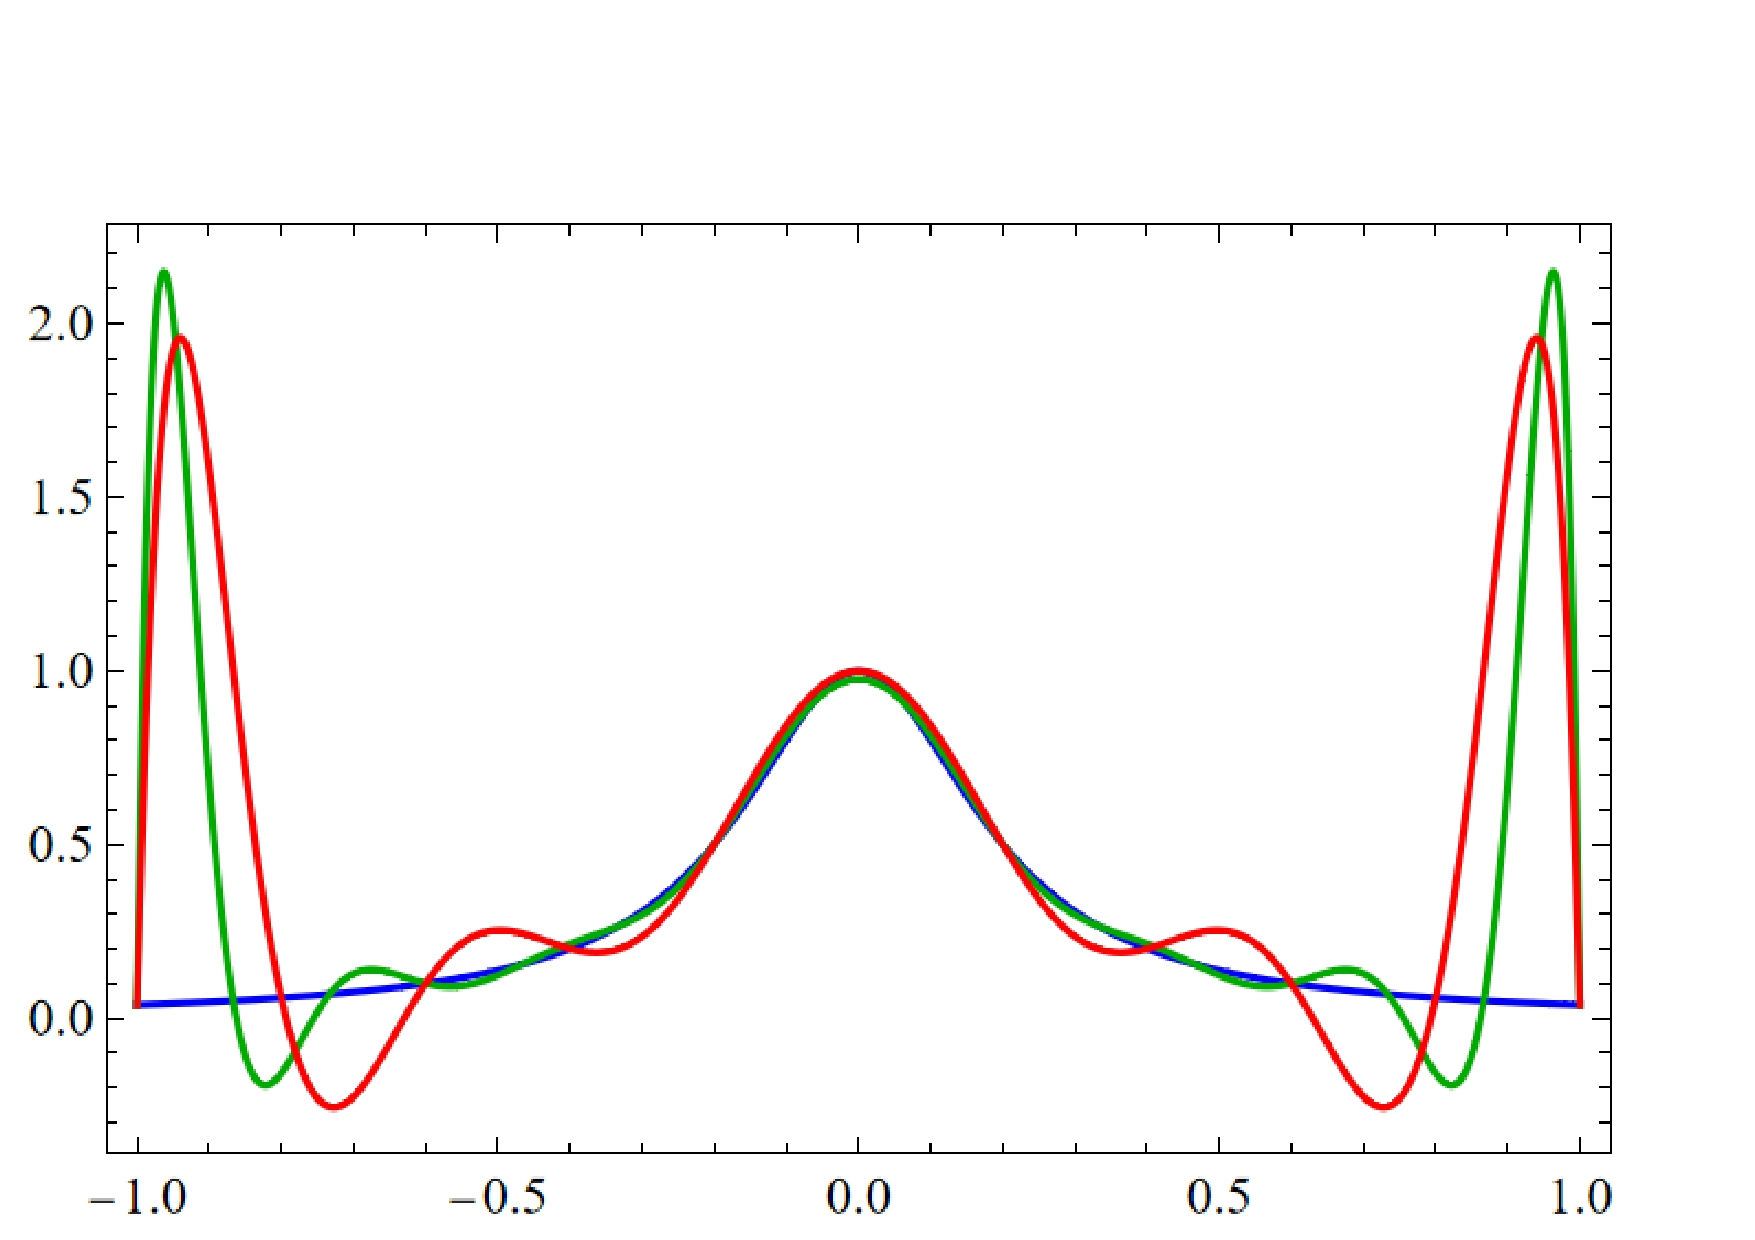
\includegraphics[scale=0.5]{runge3_page-0001.jpg}
            \caption{Fenómeno de Runge}
            \label{fig:runge}
        \end{figure}
    
        \end{obs}
        \begin{cor}
        Si analizamos el máximo del error de interpolación en todo el intervalo $I$ tenemos que
        $$\underset{x\in I}{\max}|f(x)-p_n(x)|=\|f(x)-p_n(x)\|_{\infty,I}=\left\|\frac{f^{(n+1)}(\xi)}{(n+1)!}\cdot \omega_n\right\|_{\infty,I}$$
        donde $\omega_n=(x-x_o)\cdots(x-x_n)$. De esta forma
        $$\underset{x\in I}{\max}|f(x)-p_n(x)|\leq \frac{\|f^{(n+1)}\|_{\infty,I}}{(n+1)!}\cdot \|\omega_n\|_{\infty,I}$$
        La forma de reducir este error es usando los nodos de Chebysev, que serán aquellos puntos que minimicen la función $\|\omega_n\|_{\infty}$.
        \end{cor}
        
        \section{Nodos de Chebyshev}
        \begin{defin}
        Fijemos el intervalo $I=[-1,1]$. Se definen los \textbf{polinomios de Chebyshev} (denotados por $T_n(x)$) por la siguiente fórmula de recurrencia:
        $$T_o(x)=1$$
        $$T_1(x)=x$$
        \begin{align}
        T_{n+1}(x)=2x\cdot T_{n}(x)-T_{n-1}(x)   
        \label{pol:cheb}
        \end{align}
        En la Figura \ref{fig:chebyshev} se han representado los primeros  $7$ polinomios de Chebyshev.
                 \begin{figure}[h]
            \centering
            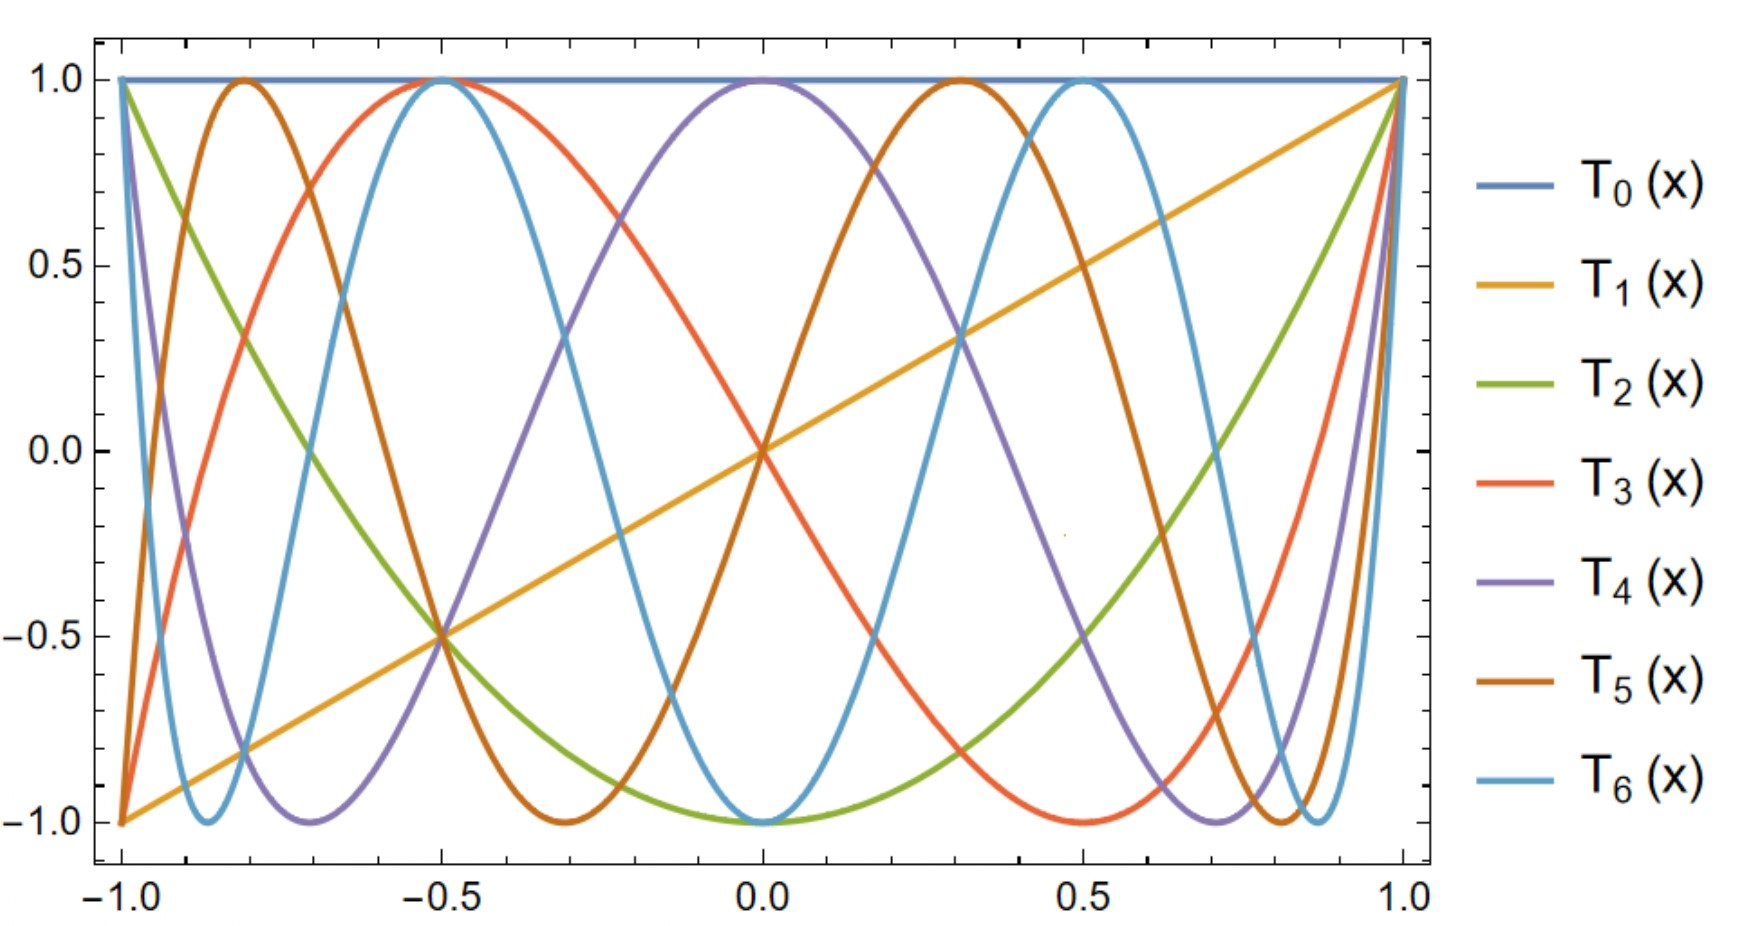
\includegraphics[scale=0.5]{chebyshev_page-0001.jpg}
            \caption{Polinomios de Chebyshev}
            \label{fig:chebyshev}
        \end{figure}
        
        \end{defin}
       
        \begin{prop}
        Para todo $x\in[-1,1]$ se verifica que
        $$T_n(\cos \theta)=\cos(n\theta)$$ o, equivalentemente, que $$T_n(x)=\cos(n\cdot \arccos(x))$$ 
        \end{prop}
        \begin{dem}
        Haremos la demostración por inducción sobre $n$. Para $n=0$ se tiene trivialmente que $1=T_o(\cos\theta)=\cos(0\cdot \theta)$.
        Supongamos que la fórmula es cierta para cierto $n\geq 0$, entonces:
        $$T_{n+1}(\cos\theta)=2\cos\theta\cdot T_n(\cos\theta)-T_{n-1}(\cos\theta)=2\cos\theta\cdot \cos(n\theta)-\cos((n-1)\theta)=$$
        $$=2\cos\theta\cdot\cos(n\theta)-(\cos(n\theta)\cdot \cos(-\theta)-\sin(n\theta)\cdot \sin(-\theta))$$
        $$=2\cos\theta\cdot\cos(n\theta)-\cos(n\theta)\cdot \cos(\theta)+\sin(n\theta)\cdot \sin(\theta))= \cos((n+1)\theta)$$
        como queríamos demostrar.
        \qed\end{dem}

        \begin{cor}\:\vspace{-5mm}
        \begin{itemize}
            \item[a)] $T_n(-x)=(-1)^n\cdot T_n(x)$
            \item[b)] El coeficiente de grado máxmo de $T_n$ es $2^{n-1}$ para $n\geq1$
            \item[c)] $\|T_n\|_{\infty,I}=1$
            \item[d)] $T_n$ tiene $n+1$ extremos en $I$.
            \item[e)] $T_n$ tiene todas sus raíces en $I$ y son distintas
        \end{itemize}
        \end{cor}

        \begin{dem}\:\vspace{-5mm}
        \begin{itemize}
            \item[a)] Por inducción sobre $n$. El caso $n=0$ es obvio. Supongamos que es cierto para algún $n\geq0$, entonces:
            $$T_{n+1}(-x)=2(-x)\cdot T_n(-x)-T_{n-1}(-x)=2(-x)\cdot (-1)^n\cdot T_n(x)-(-1)^{n-1}T_{n-1}(x)=$$
            $$=(-1)^{n-1}(2x\cdot T_n(x)-T_{n-1}(x))=(-1)^{n+1}T_{n+1}(x)$$
            \item[b)] De nuevo por inducción sobre $n$. Para $n=1$ es cierto por ser el coeficiente de mayor grado $1=2^0$. Supongamos que para cierto $n\geq 1$ se verifica que el coeficiente de mayor grado de $T_n$ es $2^{n-1}$, es decir, que $$T_{n}=2^{n-1}x^n+r_1(x)$$
            donde $r_1(x)$ denota los términos de grado menor que $n$. Se tiene entonces que
            $$T_{n+1}=2x\cdot T_n-T_{n-1}=2^nx^{n+1}+r_2(x)+T_{n-1}(x)$$
            como los grados de $r_2(x)=2x\cdot r_1(x)$ y $T_{n-1}(x)$ son menores o iguales que $n$, el coeficiente de mayor grado de $T_{n+1}$ es $2^n$ como queríamos demostrar.
            \item[c)] Como $T_n(\cos\theta)=\cos(n\theta)$ se tiene que
            $$\|T_n(\cos\theta)\|_{\infty,I}=\|\cos(n\theta)\|_{\infty,I}\leq 1$$
            \item[d)] Sabemos que $\underset{x\in I}{\max}|T_n(x)|=1$, luego basta con encontrar los $x\in I$ que verifiquen $T_n(x)=\pm 1$:
            $$T_n(x)=T_n(\cos\theta)=\cos(n\theta)=\pm1$$
            y esto solo ocurre cuando $n\theta=k\pi$ con $k\in\mathbb{Z}$, es decir, $\theta=k\cdot\frac{\pi}{n}$. Podemos decir entonces que $T_n(x'_k)=\pm 1$ cuando $x'_k=\cos\left(k\cdot\frac{\pi}{n}\right)$, $k=0,\ldots,n$, que serán $n+1$ puntos como queríamos demostrar. Además:
            $$T_n(x_{k+1})=\cos\left(\frac{\pi}{2}(2(k+1)+1)\right)=\cos\left(k\pi +\frac{3\pi}{2}\right)=\cos(k\pi)$$
            $$T_n(x_k)=\cos\left(\frac{\pi}{2}(2k+1)\right)=\cos\left(k\pi+\frac{\pi}{2}\right)=-\cos(k\pi)$$
            luego $T_n(x'_{k+1})=-T_n(x'_k)$.
            \item[e)] Como hemos visto, en el intervalo $[x'_{k+1},x'_{k}]$ se verifica que $T_n(x'_{k+1})=-T_n(x'_k)$. Aplicando el Teorema de Bolzano, $T_n(x)$ tiene una raíz en cada intervalo $[x'_{k+1},x'_{k}]$. En total habrá $n$ raíces y como $T_n(x)$ es de grado $n$, serán todas.

            Estas raíces las podemos calcular resolviendo la ecuación
            $$T_n(\cos\theta)=\cos(n\theta)=0\Longleftrightarrow n\theta=\frac{\pi}{2}+k\pi\qquad k\in\mathbb{Z}$$
            con lo cual, $\theta=\frac{\pi}{2n}(2k+1)$ con $k\in\mathbb{Z}$ y las raíces de los polinomios de Chebyshev serán entonces
            $$x_k=\cos\left(\frac{\pi}{2n}(2k+1)\right)\qquad k\in \mathbb{Z}$$
        \end{itemize}
        \qed\end{dem}
        \begin{defin}
        Denominaremos \textbf{nodos de Chebyshev} a las raíces de los polinomios de Chebyshev. Como acabamos de demostrar, en el intervalo $[-1,1]$ vienen dados por la expresión:
        \begin{align}
        x_k=\cos\left(\frac{\pi}{2n}(2k+1)\right)\qquad k\in \mathbb{Z}
        \label{nodos:cheb}
        \end{align}
        \end{defin}
        \begin{teo}
        El polinomio de Chebysev $T_n(x)$ es el polinomio con la norma infinto mínima en el intervalo $[-1,1]$ entre todos los polinomios de grado $n$ y coeficiente de grado máximo $2^{n-1}$. En otras palabras, si denotamos por $T_n'(x)=\frac{1}{2^{n-1}}T_n(x)$ entonces
        $$\|T_n'\|_{\infty,I}<\|p_n\|_{\infty,I}$$
        donde $p_n$ es cualquier polinomio de grado $n$ y mónico.
        \end{teo}
        \begin{dem}
        Sea $p_n(x)$ un polinomio mónico de grado $n$ tal que
        $$\|p_n\|_{\infty,I}\leq\|T_n'\|_{\infty,I}$$
        Por el corolario anterior, $T'_n(x)$ tiene sus extremos en los puntos $x'_k=\cos\left(k\cdot\frac{\pi}{n}\right)$ y, por tanto
        $$T'_n(x'_k)=\frac{\pm 1}{2^{n-1}}$$
        Observemos entonces que
        $$\frac{1}{2^{n-1}}=T'_n(x'_o)>p_n(x'_o)$$
        $$\frac{-1}{2^{n-1}}=T'_n(x'_1)<p_n(x'_1)$$
        $$\frac{1}{2^{n-1}}=T'_n(x'_2)>p_n(x'_2)$$
        $$\vdots$$
        En cualquier caso, el polinomio  diferencia $T'_n-p_n$ tiene signo contrario en los extremos de cada uno de los intervalos $[x'_{k+1},x'_k]$. Aplicando el Teorema de Bolzano podemos concluir que $T'_n-p_n$ tiene una raíz en cada intervalo, esto es, tiene $n$ raíces. Sin embargo, $T'_n-p_n$ es de grado $n-1$ ya que ambos son polinomios mónicos, lo cual no es posible y por tanto, no existe el polinomio $p_n(x)$.
        \qed\end{dem}
        \begin{cor}
        Sea $p_n$ el polinomio de interpolación de $f$ en los nodos de Chebysev $\{x_o,\ldots,x_n\}$. Para cada $x\in[-1,1]$ se tiene que
        $$|f(x)-p_n(x)|\leq\frac{\|f^{(n+1)}\|_{\infty,I}}{(n+1)!}\left\|\prod_{k=0}^n(x-x_k)\right\|_{\infty,I}$$
    el productorio del miembro derecho es precisamente el polinomio de Chebysev de grado $n$ multiplicado por un factor de $\frac{1}{2^{n-1}}$, con lo cual:
    $$|f(x)-p_n(x)|\leq \frac{\|f^{(n+1)}\|_{\infty,I}}{2^{n-1}(n+1)!}$$
        \end{cor}
        \begin{ejem}

        Siguiendo el ejemplo de la \textit{Observación} (pág. 23), calculemos el polinomio de interpolación de grado $15$ de la función $f(x)=\frac{1}{25x^2+1}$ utilizando los nodos de Chebyshev. El resultado se expone en la Figura \ref{fig:chebyshev2}, donde se puede apreciar que el fenómeno de Runge se ha reducido al mínimo.
        \begin{figure}[h]
            \centering
            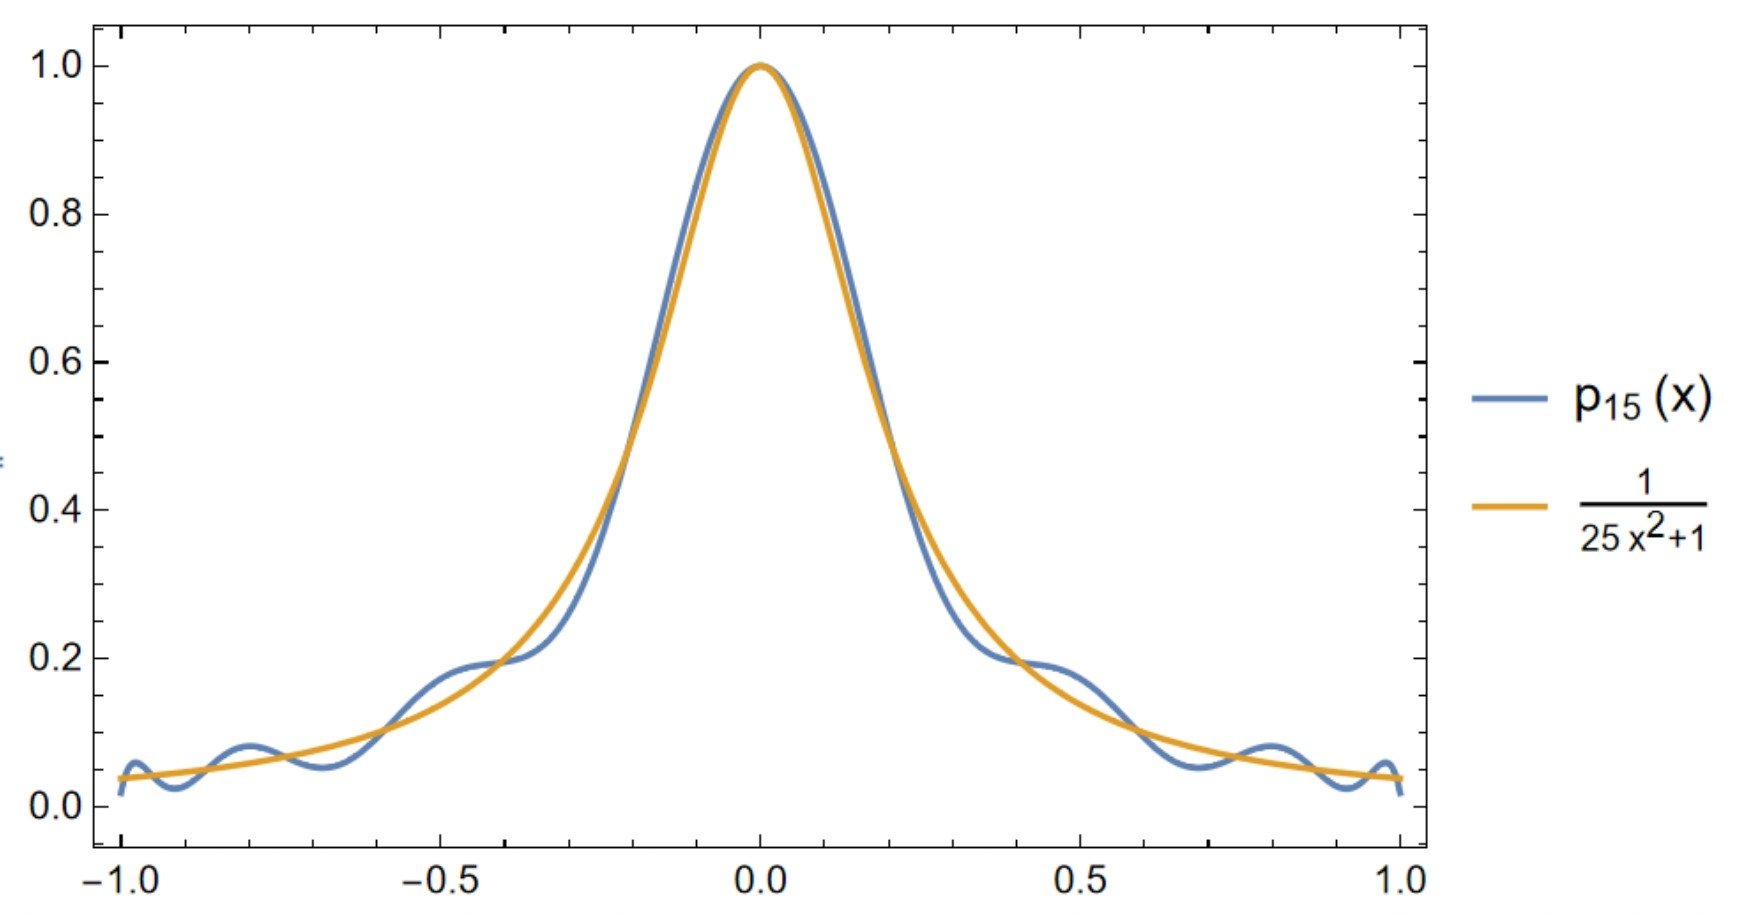
\includegraphics[scale=0.5]{chebyshev2_page-0001 (1).jpg}
            \caption{Polinomio de interpolación utilizando los nodos de Chebyshev}
            \label{fig:chebyshev2}
        \end{figure}
        \end{ejem}
        \begin{obs}
        El estudio que hemos realizado sobre los nodos de Chebyshev en el intervalo $[-1,1]$ es también válido para cualquier intervalo de la recta real. Dado el intervalo $[a,b]$, hacemos el cambio de variable
        $$\psi(t)=\frac{a+b}{2}+t\frac{b-a}{2}\qquad t\in [-1,1]$$
        para transformar el intervalo $[-1,1]$ en el intervalo $[a,b]$. Por tanto, dada una función cualquiera $f:[a,b]\longrightarrow \mathbb{R}$ podemos definir la función $f\circ\psi=\psi^*f:[-1,1]\longrightarrow\mathbb{R}$ .

        De esta manera, $\|f\|_{\infty,I}=\|\psi^*f\|_{\infty,I}$. Sean entonces $t_o,\ldots,t_n$ los nodos de Chebysev en $[-1,1]$ y $x_o,\ldots,x_n$ sus transformados por $\psi$, $x_k=\psi(t_k)$. Si $p_n$ es el polinomio de interpolación de $f$ en $\{x_0,\ldots,x_n\}$ se tiene que
        $$|f(x)-p_n(x)|\leq\frac{\|f^{(n+1)}\|_{\infty,I}}{(n+1)!}\left\|\prod_{k=0}^n(x-x_k)\right\|_{\infty,I}=$$
        $$=\frac{\|f^{(n+1)}\|_{\infty,I}}{(n+1)!}\left\|\prod_{k=0}^n\left(\frac{a+b}{2}+t\frac{b-a}{2}\right)-\left(\frac{a+b}{2}+t_k\frac{b-a}{2}\right)\right\|_{\infty,I}=\frac{\|f^{(n+1)}\|_{\infty,I}}{(n+1)!}\left\|\prod_{k=0}^n(t-t_k)\left(\frac{b-a}{2}\right)\right\|_{\infty,I}\leq$$
        $$\leq \frac{\|f^{(n+1)}\|_{\infty,I}}{(n+1)!}\cdot\frac{(b-a)^{n+1}}{2^{2n}}$$
        \end{obs}
        \section{Fórmulas de Newton-Gregory}
        \begin{defin}
        Dada una colección de nodos $\{x_o,\ldots,x_n\}$ diremos que están \textbf{equiespaciados o equidistantes} si $x_{i+1}=x_i +h$ para cierto $h>0$.
        \end{defin}
        \begin{defin}
        Sean $\{x_o,\ldots,x_n\}$ $n+1$ puntos distintos y $f:\mathbb{R}\longrightarrow\mathbb{R}$. Denominaremos \textbf{operador diferencia progresiva} al siguiente operador:
        $$\Delta f(x_i)=f(x_{i+1})-f(x_i)$$
        Equivalentemente, se define el \textbf{operador diferencia regresiva} como sigue
        $$\nabla f(x_i)=f(x_i)-f(x_{i-1})$$
        \end{defin}
        \begin{prop}
        Para todo $n\geq1$ se verifica que
        $$\Delta^n f(x_o)=\nabla ^n f(x_n)=\sum_{k=0}^n \binom{n}{k} (-1)^k f(x_{n-k})$$
        \end{prop}
        \begin{dem}
        Demostraremos la fórmula para el operador diferencia progresiva por inducción sobre $n$. Para $n=1$ la fórmula es cierta por definición. Supongamos entonces que se verifica para $n-1$ y estudiemos el siguiente caso:
        $$\Delta^n f(x_o)=\Delta(\Delta^{n-1}f(x_o))=\Delta\left(\sum_{k=0}^{n-1} \binom{n-1}{k} (-1)^kf(x_{n-k-1})\right)=$$
        $$=\sum_{k=0}^{n-1} \binom{n-1}{k} (-1)^k f(x_{n-k})-\sum_{k=0}^{n-1} \binom{n-1}{k} (-1)^kf(x_{n-k-1})$$
        Haciendo el cambio de índice $k\to k-1$ en el segundo sumatorio obtenemos lo siguiente:
        $$\Delta^n f(x_o)=f(x_n)+\sum_{k=1}^{n-1}\binom{n-1}{k} (-1)^k f(x_{n-k})+\sum_{k=1}^{n-1}\binom{n-1}{k-1} (-1)^k  f(x_{n-k})+(-1)^n f(x_o)=$$
        $$=f(x_n)+\sum_{k=1}^{n-1}\left(\binom{n-1}{k}+\binom{n-1}{k-1}\right)(-1)^k f(x_{n-k})+(-1)^n f(x_o)=\sum_{k=0}^n \binom{n}{k} (-1)^k f(x_{n-k})$$
        Análogamente se demuestra para el operador diferencia regresiva.
        \qed\end{dem}
        \begin{prop}
        Dados $n+1$ nodos equiespaciados $\{x_o,\ldots,x_n\}$ se tiene que
        $$f[x_o,\ldots,x_n]=\frac{\Delta^n f(x_o)}{n! h^n}=\frac{\nabla^n f(x_n)}{n! h^n}$$
        \end{prop}
        \begin{dem}
        Veamos primero el caso del operador diferencia progresiva por inducción sobre $n$. Para $n=1$ la fórmula es cierta ya que
        $$f[x_o,x_1]=\frac{f(x_1)-f(x_o)}{x_1-x_o}=\frac{\Delta f(x_o)}{h}$$
        Supongamos entonces que la fórmula es cierta para $n-1$, veamos qué ocurre para $n$:
        $$f[x_o,\ldots,x_n]=\frac{f[x_1,\ldots,x_n]-f[x_o,\ldots,x_{n-1}]}{x_n-x_o}=\frac{\frac{\Delta^{n-1} f(x_1)}{(n-1)! h^{n-1}}-\frac{\Delta^{n-1} f(x_o)}{(n-1)! h^{n-1}}}{nh}=$$
        $$=\frac{\Delta^{n-1}f(x_1)-\Delta^{n-1}f(x_o)}{n!h^n}=\frac{\Delta^n f(x_o)}{n! h^n}$$
        Como las diferencias divididas son invariantes bajo permutaciones, podemos hacer el cambio de índice $i\to n-i$ (que es una permutación por ser una biyección). Para $n=1$ se tiene que
        $$f[x_o,x_1]=f[x_1,x_o]=\frac{f(x_o)-f(x_1)}{x_0-x_1}=\frac{\nabla f(x_1)}{h}$$
        Supongamos ahora que la fórmula es cierta para $n-1$
        $$f[x_o,\ldots,x_n]=\frac{f[x_1,\ldots,x_n]-f[x_o,\ldots,x_{n-1}]}{x_n-x_o}=\frac{\frac{\nabla^{n-1} f(x_n)}{(n-1)! h^{n-1}}-\frac{\nabla^{n-1} f(x_{n-1})}{(n-1)! h^{n-1}}}{nh}=$$
        $$=\frac{\nabla^{n-1}f(x_n)-\nabla^{n-1}f(x_{n-1})}{n!h^n}=\frac{\nabla^n f(x_n)}{n! h^n}$$
        \qed\end{dem}
        \begin{teo}
        (\textbf{Fórmula de Newton-Gregory progresiva)} Si denotamos por $p_n(x)$ al polinomio de interpolación de una función $f$ en los nodos equiespaciados $\{x_o,\ldots,x_n\}$ se tiene que
        \begin{align}
        p_n(x)=\sum_{i=0}^n\binom{s}{i}\Delta^i f(x_o)
        \label{newton-gregoryprog}
        \end{align}
        donde $s=\dfrac{x-x_o}{h}$. 
        \end{teo}
        \begin{dem}
        Sabemos que el polinomio de interpolación de Newton en $\{x_o,\ldots,x_n\}$ se puede expresar de la siguiente forma:
        $$p_n(x)= f(x_o)+\sum_{i=1}^n f[x_o,\ldots,x_i](x-x_o)\cdots(x-x_{i-1})$$
        Aplicando ahora la proposición anterior 
        $$p_n(x)=f(x_o)+\sum_{i=1}^n\frac{\Delta^i f(x_o)}{i! h^i} (x-x_o)\cdots(x-x_{i-1})=$$
        $$=f(x_o)+\sum_{i=1}^n\frac{\Delta^i f(x_o)}{i! h^i} (x-x_o)(x-x_o-h)\cdots(x-x_o-h(i-1))=$$
        $$=f(x_o)+\sum_{i=1}^n\frac{\Delta^i f(x_o)}{i!} \left(\frac{x-x_o}{h}\right)\left(\frac{x-x_o}{h}-1\right)\cdots\left(\frac{x-x_o}{h}-(i-1)\right)$$
       
        Tomando $s=\dfrac{x-x_o}{h}$ obtenemos lo siguiente
        $$p_n(x)=f(x_o)+\sum_{i=1}^n \Delta^i f(x_o)\dfrac{s(s-1)\cdots(s-(i-1))}{i!}=f(x_o)+\sum_{i=1}^n \Delta^i f(x_o)\dfrac{s!}{i!(s-i)!}=\sum_{i=0}^n\binom{s}{i}\Delta^i f(x_o)$$
        \qed\end{dem}
        \begin{teo}
        (\textbf{Fórmula de Newton-Gregory regresiva}) Si denotamos por $p_n(x)$ al polinomio de interpolación de una función $f$ en los nodos equiespaciados $\{x_o,\ldots,x_n\}$ se tiene que
        \begin{align}
        p_n(x)=\sum_{i=0}^n\binom{u+i-1}{i}\nabla^i f(x_n)
        \label{newton-gregoryreg}
        \end{align}
        donde $u=\dfrac{x-x_n}{h}$. 
        
        \end{teo}
        \begin{dem}

        El polinomio de interpolación de $f$ en los nodos $\{x_o,\ldots,x_n\}$ es el mismo que en los nodos $\{x_n,\ldots,x_0\}$, con lo cual:
        $$p_n(x)=f(x_n)+\sum_{i=1}^nf[x_n,\ldots,x_{n-i}](x-x_n)\cdots(x-x_{n-i-1})$$
        Como los nodos son equiespaciados, sabemos que $x_i=x_n-ih$. Aplicando además la proposición anterior y la invariancia de las diferencias divididas bajo permutaciones se tiene que
        $$p_n(x)=f(x_n)+\sum_{i=1}^n\frac{\nabla^i f(x_n)}{i! h^i}(x-x_n)(x-x_n+h)\cdots(x-x_n+(i-1)h)=$$
        $$=f(x_n)+\sum_{i=1}^n\frac{\nabla^i f(x_n)}{i!} \left(\frac{x-x_n}{h}\right)\left(\frac{x-x_n}{h}+1\right)\cdots\left(\frac{x-x_n}{h}+(i-1)\right)$$
        Tomando $u=\dfrac{x-x_n}{h}$ obtenemos lo siguiente
        $$p_n(x)=f(x_n)+\sum_{i=1}^n\nabla^if(x_n)\frac{u(u+1)\cdots(u+(i-1))}{i!}=f(x_n)+\sum_{i=1}^n\nabla^if(x_n)\frac{(u+i-1)!}{i!((u+i-1)-i)!}=$$
        $$=\sum_{i=0}^n\binom{u+i-1}{i}\nabla^i f(x_n)$$
                
        \qed\end{dem}
        \section{Interpolación de Hermite}
        \begin{defin}
        Sea $f$ una función de variable real y $\{(x_o,\alpha_o),\ldots,(x_s,\alpha_s)\}$ donde $x_0,\ldots,x_s$ son $s+1$ nodos distintos y $\alpha_o,\ldots,\alpha_s$ son $s+1$ números naturales (a los que denominaremos multiplicidades). Diremos que un polinomio $p_n(x)$ \textbf{interpola} (en el sentido de Hermite) a $f$ cuando
        $$f^{(\beta_i)}(x_i)=p_n^{(\beta_i)}(x_i)\qquad 0\leq \beta_i\leq\alpha_i$$
        \end{defin}
        \begin{obs}
        El grado del polinomio de interpolación de Hermite en $\{(x_o,\alpha_o),\ldots,(x_n,\alpha_n)\}$ es
        $$n=\left(\sum_{i=0}^s\alpha_i +s+1\right)-1=\sum_{i=0}^s\alpha_i +s$$
         \end{obs}
        \begin{ejem}
        Dos ejemplos interesantes de la interpolación de Hermite son para $\alpha_i=0$ (interpolación de Lagrange) y para $s=0$, donde el resultado es el polinomio de Taylor.
        
        \end{ejem}
        \begin{teo}
        Sea $f$ una función de variable real y $\{(x_o,\alpha_o),\ldots,(x_n,\alpha_n)\}$ el conjunto de nodos con sus respectivas multiplicidades. Entonces existe un único polinomio $p_n$ de grado $n=\sum_{i=0}^s\alpha_i +s$ tal que
        $$f^{(\beta_i)}(x_i)=p_n^{(\beta_i)}(x_i)\qquad 0\leq \beta_i\leq\alpha_i$$
        \end{teo}
        \begin{dem}
        Consideremos la siguiente aplicación:
        $$\begin{array}{rrcl}
        \varphi_n:&\mathbb{P}_n[x]     &\longrightarrow & \mathbb{R}^{n+1}  \\
          &p(x)   &\longmapsto & (p(x_o),p'(x_o),\ldots,p^{(\alpha_o)}(x_o),\ldots, p(x_s),p'(x_s),\ldots,p^{(\alpha_s)}(x_s) )
        \end{array}$$
        Sabemos que $\varphi_n$ es una aplicación lineal por las propiedades de la derivada. Sea $p(x)\in Ker \,\varphi_n$, es decir, $p_n^{(\beta_i)}(x_i)=0$ para cualesquiera $i,\beta_i$. Por tanto,  $p_n(x)$ es múltiplo de$(x-x_i)^{\alpha_i+1}$. Entonces:
        $$p(x)=\lambda (x-x_o)^{\alpha_o+1}\cdots(x-x_s)^{\alpha_s+1}$$
        y como el polinomio del miembro izquierdo es de grado $n$ y el del derecho de grado $\sum_{i=0}^s(\alpha_i+1)=n+1$,  necesariamente $\lambda=0$ y, con lo cual, $\varphi_n$ es inyectiva. Por cómputo de dimensiones podemos concluir que $\varphi_n$ es isomorfismo.

        Esto nos basta para concluir la demostración, ya que el polinomio $p_n$ buscado será\newline $\varphi^{-1}(f(x_o),f'(x_o),\ldots,f^{(\alpha_o)}(x_o),\ldots, f(x_s),f'(x_s),\ldots,f^{(\alpha_s)}(x_s) )$.
        \qed\end{dem}
        \begin{obs}
        El hecho de que $\varphi_n$ sea isomorfismo implica que las formas lineales  $\omega_i^{\beta_i}$ definidas por $\omega_i^{\beta_i}(p)=p^{(\beta_i)}(x_i)$ forman una base de $\mathbb{P}_n^*[x]$. Su base dual serán los \textbf{polinomios de interpolación de Hermite}, a los que denotaremos por $h_i^{\beta_i}$. Por el teorema de la base dual, el polinomio de interpolación de Hermite en esta base será de la forma
        $$p_n(x)=\sum_{i=0}^s\sum_{\beta_i=0}^{\alpha_i}\omega_i^{\beta_i}(p_n)\cdot h_i^{\alpha_i}=\sum_{i=0}^s\sum_{\beta_i=0}^{\alpha_i}f^{(\beta_i)}(x_i)\cdot h_i^{\beta_i}$$
        \end{obs}
        \begin{prop}
        Con las notaciones precedentes, se tiene que
        \begin{align}
        h_i^{\alpha_i}=\frac{1}{\alpha_i!}(x-x_i)^{\alpha_i}\prod_{j\neq i}\left(\frac{x-x_j}{x_i-x_j}\right)^{\alpha_j+1}
        \label{pol:herm}
        \end{align}
        y el resto de polinomios se calculan recursivamente por la fórmula
        $$h_i^{\alpha_i-j}=\tilde{h}_i^{\alpha_i-j}-\sum_{k=1}^jc_{i,\alpha_i-j,\alpha_i-j+k}\cdot h_i^{\alpha_i-j+k}$$
        donde
        $$\tilde{h}_i^{\alpha_i-j}=\frac{1}{(\alpha_i-j)!}(x-x_i)^{\alpha_i-j}\prod_{k\neq i}\left(\frac{x-x_k}{x_i-x_k}\right)^{\alpha_k+1}$$
        $$c_{i,\alpha_i-j,\alpha_i-j+k}=(\tilde{h}_i^{\alpha_i-j})^{(\alpha_i-j+k)}(x_i)$$
        \end{prop}
        \begin{dem}
        Por ser la base dual de $\omega_i^{\beta_i}$, sabemos que los polinomios $h_i^{\beta_i}$ verifican lo siguiente:
        $$(h_i^{\beta_i})^{\beta_j}(x_j)=\left\{\begin{array}{cc}
           0  & j\neq i \\
            0 & j=i, \,\beta_i\neq \beta_j\\
            1 & j=i,\, \beta_i=\beta_j
        \end{array}\right.$$
        Construyamos $h_i^{\alpha_i}(x)$. Sean $\Omega(x)=\prod_{j=1}^s(x-x_j)^{\alpha_j+1}$ y $\Omega_i(x)=\dfrac{\Omega}{(x-x_i)^{\alpha_i+1}}$. 
        
        Como $(h_i^{\alpha_i})^{\beta_j}(x_j)=0$, necesariamente $h_i^{\alpha_i}$ es múltiplo de $\Omega_i$. Además, como \newline $(h_i^{\alpha_i})^{\beta_i}(x_i)=0$ con $\beta_i\leq\alpha_i-1$, deducimos también que $h_i^{\alpha_i}$ es múltiplo de $(x-x_i)^{\alpha_i}$. En conclusión
        $$h_i^{\alpha_i}(x)=C \cdot\Omega_i(x)(x-x_i)^{\alpha_i}$$
        El grado del polinomo de la derecha es
        $$\alpha_i+\sum_{\underset{j\neq i}{j=0}}^s(\alpha_j+1)=n$$
        Luego por cómputo de dimensiones se tiene que $C\in \mathbb{R}$.      Finalmente, determinaremos $C$ por la condición $(h^{\alpha_i})^{(\alpha_i)}(x_i)=1$
        $$(h^{\alpha_i})^{(\alpha_i)}(x_i)= C\left(\sum_{k=0}^{\alpha_i}\binom{\alpha_i}{k}\dfrac{d^k}{dx^k}(x-x_i)^{\alpha_i}\cdot\dfrac{d^{\alpha_i-k}}{dx^{\alpha_i-k}}\Omega_i(x)\right)(x_i)= $$
        $$=C\cdot \alpha_i!\cdot \Omega_i(x_i)+\left(\sum_{k=0}^{\alpha_i-1}\binom{\alpha_i}{k}\dfrac{d^k}{dx^k}(x-x_i)^{\alpha_i}\cdot\dfrac{d^{\alpha_i-k}}{dx^{\alpha_i-k}}\Omega_i(x)\right)(x_i)$$
        Como $\dfrac{d^k}{dx^k}(x-x_i)^{\alpha_i}$ es múltiplo de $(x-x_i)$ cuando $k\leq \alpha_i-1$, el sumatorio anterior se anula al evaluarlo en $x=x_i$. Por tanto:
        $$C=\dfrac{1}{\alpha_i!\cdot \Omega_i(x_i)}$$
        y en efecto 
        $$h_i^{\alpha_i}=\frac{1}{\alpha_i!}(x-x_i)^{\alpha_i}\prod_{j\neq i}\left(\frac{x-x_j}{x_i-x_j}\right)^{\alpha_j+1}$$
Sea ahora $w_i(x)=\prod_{j\neq i}\left(\frac{x-x_j}{x_i-x_j}\right)^{\alpha_j+1}$ y consideremos el polinomio
$$\tilde{h}_i^{\alpha_i-1}(x)=\dfrac{1}{(\alpha_i-1)!}(x-x_i)^{\alpha_i-1}\cdot w_i(x)$$
Veamos si el polinomio $h_i^{\alpha_i}$ definido por
$$h_i^{\alpha_i-1}=\tilde{h}_i^{\alpha_i-1}-c_{i,\alpha_i-1,\alpha_i-j}\cdot h_i^{\alpha_i}$$
con $(\tilde{h}_i^{\alpha_i-1})^{(\alpha_i)}(x_i)=
c_{i,\alpha_i-1,\alpha_i}$ verifica las condiciones necesarias. 

Comprobemos primero si $(h_i^{\alpha_i-1})^{(\beta_j)}(x_j)=0$. Como $(h_i^{\alpha_i})^{(\beta_j)}(x_j)=0$, basta con ver que $(\tilde{h}_i^{\alpha_i-1})^{\beta_j}(x_j)=0$, lo cual es cierto porque $\dfrac{d}{dx^k}\omega_i(x)$ se anula en $x=x_j$ siempre que $k\leq \alpha_j$.

Por otro lado:
$$(h_i^{\alpha_i-1})^{(\beta_j)}(x_i)=(\tilde{h}_i^{\alpha_i-1})^{\beta_j}(x_i)-c_{i,\alpha_i-j,\alpha_i}\cdot (h_i^{\alpha_i})^{(\beta_j)}(x_i)$$
Si $\beta_j=\alpha_i$
$$(h_i^{\alpha_i-1})^{(\alpha_j)}(x_i)=c_{i,\alpha_i-j,\alpha_i}-c_{i,\alpha_i-j,\alpha_i}\cdot 1=0$$
Y si $\beta_j<\alpha_i-1$
$(h_i^{\alpha_i-1})^{(\beta_j)}(x_i)=(\tilde{h}_i^{\alpha_i-1})^{(\beta_j)}(x_i)$
y por la misma razón que antes, la derivada anterior será un múltiplo de $(x-x_i)$, luego nula en $x=x_i$. Por último, veamos si $(h_i^{\alpha_i-1})^{(\alpha_i-1)}=1$
$$(h_i^{\alpha_i-1})^{(\alpha_i-1)}(x_i)=(\tilde{h}_i^{\alpha_i-1})^{(\alpha_i-1)}(x_i)=\dfrac{1}{(\alpha-1)!}\left(\sum_{k=0}^{\alpha_i-1}\binom{\alpha_i-1}{k}\dfrac{d^k}{dx^k}(x-x_i)^{\alpha_i-1}\cdot\dfrac{d^{\alpha_i-1-k}}{dx^{\alpha_i-1-k}}w_i(x)\right)(x_i)=$$
$$=\dfrac{1}{(\alpha-1)!}\left((\alpha-1)! w_i(x)+\sum_{k=0}^{\alpha_i-2}\binom{\alpha_i-1}{k}\dfrac{d^k}{dx^k}(x-x_i)^{\alpha_i-1}\cdot\dfrac{d^{\alpha_i-1-k}}{dx^{\alpha_i-1-k}}w_i(x)\right)(x_i)$$
Como $w_i(x_i)=1$ y el sumatorio se anula al tomar $x=x_i$, obtenemos la conclusión deseada. La demostración de la fórmula recursiva  se hace por inducción (mucha suerte para el que lo intente).
\qed\end{dem}
       
 
        
      \subsection{Diferencias divididas generalizadas}
      \begin{prop}
      Sea $p_n(x)$ el polinomio de interpolación de Hermite de una función $f$ en los nodos $\{(x_o,\alpha_o),\ldots,(x_s,\alpha_s)\}$, entonces existe una constante $c_n$ tal que
      \begin{align}
      p_n(x)=p_{n-1}(x)+c_n\cdot (x-x_o)^{\alpha_o+1}\cdots (x-x_{s-1})^{\alpha_{s-1}+1}(x-x_s)^{\alpha_s}
     \label{hermite:newton} \end{align}
      donde $p_{n-1}$ es el polinomio de interpolación de Hermite de $f$ en los nodos $\{(x_o,\alpha_o),\ldots,(x_{s-1},\alpha_{s-1})\}\cup \{(x_s,\alpha_s-1)\}$($:=\emptyset$ si $\alpha_s-1=0$). Esta es la \textbf{fórmula de Newton para el polinomio de interpolación de Hermite}.
      \end{prop}
      \begin{dem}
      Consideremos el polinomio $q_n(x)=p_n(x)-p_{n-1}(x)$. Por las definiciones de $p_n(x)$ y $p_{n-1}(x)$ sabemos que $(q_n(x))^{(\beta_i)}(x_i)=0$ con $i\neq s$ y $0\leq \beta_i\leq\alpha_i$, lo cual implica que $q_n(x)$ es múltiplo de $\prod_{i=0}^{s-1}(x-x_i)^{\alpha_i+1}$. Además, también se verifica que $(q_n(x))^{(\beta_s)}(x_s)=0$ siempre y cuando $0\leq \beta_s<\alpha_s$, luego $q_n(x)$ es múltiplo de $(x-x_s)^{\alpha_s}$. Por tanto:
      $$q_n(x)=\lambda\cdot \prod_{i=0}^{s-1}(x-x_i)^{\alpha_i+1}(x-x_s)^{\alpha_s}$$
      El grado del polinomio del miembro derecho será
      $$\sum_{i=0}^{s-1}(\alpha_i+1)+\alpha_s=s+\sum_{i=0}^{s}\alpha_i=n$$
      por cómputo de dimensiones $\lambda\in\mathbb{R}$ y $c_n=\lambda$.
      \qed\end{dem}
      \begin{defin}
    Sean $\{x_o,\ldots,x_n\}$ $n+1$ puntos ordenados ($x_o\leq x_1\leq \ldots\leq x_n$) y $f$ una función $n$ veces diferenciable. Se definen las \textbf{diferencias divididas generalizadas} por la siguiente recurrencia:
    $$f[x_o]=f(x_o)$$
    
    $$f[x_o,x_1]=\left\{\begin{array}{cc}
       \dfrac{f(x_1)-f(x_o)}{x_1-x_o}  &\text{si }x_1\neq x_o  \\
       \vspace{-5mm} & \\
         f'(x_o) & \text{si }x_1= x_o
    \end{array}\right.$$
    \begin{align}
    f[x_o,\ldots,x_n]=\left\{\begin{array}{cc}
       \dfrac{f[x_1,\ldots,x_n]-f[x_o,\ldots,x_{n-1}]}{x_n-x_o}  &\text{si }x_n\neq x_o  \\
       & \\
         \dfrac{f^{(n)}(x_o)}{n!} & \text{si }x_n= x_o
    \end{array}\right.
    \label{difdiv:gen}
    \end{align}
      \end{defin}
      \begin{obs}
      La motivación de la definición $f[x_i,x_i]=f'(x_i)$ viene de la propia definición de derivada:
      $$f'(x_i)=\lim_{x\to x_i}\frac{f(x_i)-f(x)}{x_i-x}$$
      \end{obs}
      \begin{teo}
    Con las notaciones precedentes, se verifica que
    $$c_n=f[x_o,\overset{(\alpha_o+1)}{\ldots},x_o,x_1,\overset{(\alpha_1+1)}{\ldots},x_1,\ldots,x_s,\overset{(\alpha_s+1)}{\ldots},x_s]$$
      \end{teo}
      \begin{dem}
    Haremos la demostración por inducción sobre $n$. Para $s=0$ el polinomio de interpolación de Hermite coincide con el de Taylor, luego la fórmula es cierta. Consideremos ahora el caso $s\neq 0$. Para $n=1$ tenemos que:
    $$\alpha_o=\alpha_1=0\Longrightarrow p_1(x)=f(x_o)+f[x_o,x_1](x-x_0)$$
    Supongamos que la fórmula es cierta para polinomios de grado $n-1$, veamos si se verifica para los de grado $n$. Sea $p_n$ el polinomio de interpolación de Hermite en $\{(x_o,\alpha_o),\ldots,(x_s,\alpha_s)\}$. Denotemos por $p_{n-1}(x)$,$\bar{p}_{n-1}(x)$ a los polinomios de interpolación de Hermite en los nodos $\{(x_o,\alpha_o),\ldots,(x_{s-1},\alpha_{s-1})\}\cup \{(x_s,\alpha_s-1)\}$ y $\{(x_1,\alpha_1),\ldots,(x_{s},\alpha_{s})\}\cup \{(x_o,\alpha_o-1)\}$ respectivamente. Por la proposición anterior, sabemos que
    $$p_n(x)=p_{n-1}(x)+c_n\cdot (x-x_o)^{\alpha_o+1}\cdots (x-x_{s-1})^{\alpha_{s-1}+1}(x-x_s)^{\alpha_s}$$
    $$p_n(x)=\bar{p}_{n-1}(x)+\bar{c}_n\cdot (x-x_o)^{\alpha_o}(x-x_1)^{\alpha_1+1}\cdots (x-x_s)^{\alpha_s+1}$$
    Por la unicidad del polinomio de interpolación de Hermite, concluimos que $c_n=\bar{c}_n$. Restando ambas ecuaciones obtenemos lo siguiente:
    $$0=\bar{p}_{n-1}-p_{n-1}+c_n((x-x_o)^{\alpha_o+1}\cdots (x-x_{s-1})^{\alpha_{s-1}+1}(x-x_s)^{\alpha_s}-(x-x_o)^{\alpha_o}(x-x_1)^{\alpha_1+1}\cdots (x-x_s)^{\alpha_s+1})=$$
    $$=c_n(x-x_1)^{\alpha_1+1}\cdots(x-x_{s-1})^{\alpha_{s-1}+1}(x-x_o)^{\alpha_o}(x-x_s)^{\alpha_s}(x_o-x_s)$$
  Comparando los coeficientes de grado máximo en ambos miembros de la igualdad y aplicando la hipótesis de inducción se tiene que
    $$0=f[x_o,\overset{(\alpha_o)}{\ldots},x_o,x_1,\overset{(\alpha_1+1)}{\ldots},x_1,\ldots,x_s,\overset{(\alpha_s+1)}{\ldots},x_s]-f[x_o,\overset{(\alpha_o+1)}{\ldots},x_o,x_1,\overset{(\alpha_1+1)}{\ldots},x_1,\ldots,x_s,\overset{(\alpha_s)}{\ldots},x_s]+c_n(x_o-x_s)$$
    y despejando se concluye .
      \qed\end{dem}

      \subsection{Error de la interpolación de Hermite}
      \begin{lem}
      Sea $f$ una función $n+1$ veces diferenciable en $(x_o,x_1)$ y $\{(x_o,\alpha_o),(x_1,\alpha_1,\ldots,(x_s,\alpha_s)\}$ con $x_o<x_1<\ldots<x_s$, se tiene que
      $$f[x_o,\overset{(\alpha_o+1)}{\ldots},x_o,x_1,\overset{(\alpha_1+1)}{\ldots},x_1,\ldots,x_s,\overset{(\alpha_s+1)}{\ldots},x_s]=\frac{f^{(n)}(\xi)}{n!}$$
      para cierto $\xi\in[x_0,x_s]$  y con $n=\sum_{i=0}^s\alpha_i+s$.
      \end{lem}
      \begin{dem}
        Denotemos por $\tau_k$ al número de nodos $x_i$ tales que $\alpha_i\geq k$ y sea \newline $m=\max\{\alpha_i\}$. Con esta notación, se tiene que $\tau_o=s+1$ por ser $\alpha_i\geq 0$. Además,
        $$\sum_{k=0}^m\tau_k=\sum_{i=0}^s(\alpha_i+1)=n+1$$
        Sea $p_n(x)$ el polinomio de interpolación de Hermite de $f$ en los nodos y multiplicidades  $\{(x_o,\alpha_o),(x_1,\alpha_1,\ldots,(x_s,\alpha_s)\}$. Consideremos la función $\mathcal{E}_n(x)=f(x)-p_n(x)$ y veamos dónde se anulan sus derivadas:

        \item[0)] $\mathcal{E}_n$ se anula en $\tau_o$ puntos por la definición del polinomio de interpolación de Hermite.
        \item[1)]$\mathcal{E}_n'(x)$ se anula en $\tau_o-1$ puntos (intermedios) por el teorema de Rolle y en $\tau_1$ nodos por la definición del polinomio de interpolación de Hermite.
        \item[2)]$\mathcal{E}_n''(x)$ se anula en $\tau_o+\tau_1+\tau_2-1-1$ puntos.
        
        $\vdots$
        
        \item[k)]$\mathcal{E}_n^{(k)}(x)$ se anula en $\tau_o+\ldots+\tau_k-k$ puntos

        Reiterando este argumento podemos deducir que $\mathcal{E}_n^{(n)}(x)$ se anula en  $\tau_o+\ldots+\tau_n-n=n+1-n=1$ punto, por ser $n\geq m$. Denotemos por $\xi$ a dicho punto. Se tiene entonces que
        $$\mathcal{E}_n^{(n)}(\xi)=f^{(n)}(\xi)-p_n^{(n)}(\xi)=f^{(n)}(\xi)-n!\cdot f[x_o,\overset{(\alpha_o+1)}{\ldots},x_o,x_1,\overset{(\alpha_1+1)}{\ldots},x_1,\ldots,x_s,\overset{(\alpha_s+1)}{\ldots},x_s]=0 $$
        y despejando se concluye.
        
      \qed\end{dem}
      \begin{teo}
        Con las notaciones precedentes, para todo $x\in[x_o,x_s]$ se verifica que
        \begin{align}
          \mathcal{E}_n(x)=\dfrac{f^{(n+1)}(\xi)}{(n+1)!}\cdot \prod_{i=0}^s(x-x_i)^{\alpha_i+1}
          \label{error:herm}
        \end{align}
        
      \end{teo}
      \begin{dem}
        Si $x=x_i$ la fórmula es cierta. Supongamos entonces que $x\neq x_i$ y sea $p_{n+1}(x)$ el polinomio de interpolación de Hermite de $f$ en $\{(x_o,\alpha_o),\ldots,(x_s,\alpha_s)\}\cup \{(x,0)\}$. Por \ref{hermite:newton} sabemos que
        $$p_{n+1}(x)=p_n(x)+c_{n+1}\prod_{i=0}^s(x-x_i)^{\alpha_i+1}$$
        con $c_{n+1}=f[x_o,\overset{(\alpha_o+1)}{\ldots},x_o,x_1,\overset{(\alpha_1+1)}{\ldots},x_1,\ldots,x_s,\overset{(\alpha_s+1)}{\ldots},x_s,x]=\dfrac{f^{(n+1)}(\xi)}{(n+1)!}$ por el lema anterior.
        Con lo cual
        $$\mathcal{E}_n(x)=f(x)-p_n(x)=p_{n+1}(x)-p_n(x)=\dfrac{f^{(n+1)}(\xi)}{(n+1)!}\cdot \prod_{i=0}^s(x-x_i)^{\alpha_i+1}$$
      \qed\end{dem}
        
        \section{Ejercicios}
        \begin{ejer}
             El porcentaje de germinación $G$ de una variedad de tomates se mide a tres temperaturas
diferentes, $T$. A 9ºC solamente germina el 20\%, a 12ºC el 40\% y a 15ºC el porcentaje es del
70\%. Encuentra una expresión de $G$ como función cuadrática de $T$ y usando dicha expresión
predice el porcentaje de germinación a 11ºC y a 13ºC. ¿A qué temperatura la germinación
será del 10\%? Comenta los resultados.
        \end{ejer}
        \begin{sol}
        Calcularemos el polinomio de interpolación de grado $2$ por el método de Lagrange. Los polinomios de Lagrange con nodos $\{9,12,15\}$ serán:
        $$\ell_o=\frac{(T-12)(T-15)}{(9-12)(9-15)}$$
        $$\ell_1=\frac{(T-9)(T-15)}{(12-9)(12-15)}$$
        $$\ell_2=\frac{(T-9)(T-12)}{(15-9)(15-12)}$$
        Y por tanto, el polinomio de interpolación buscado es
        $$p_2(x)=\frac{(T-12)(T-15)}{(9-12)(9-15)}\cdot 20+\frac{(T-9)(T-15)}{(12-9)(12-15)}\cdot 40+\frac{(T-9)(T-12)}{(15-9)(15-12)}\cdot 70=$$
        Podemos concluir por tanto que el porcentaje de germinación a 11ºC
 será aproximadamente $p(11)\approx 32\% $. No podemos decir nada sobre la temperatura a la cual la germinación es del 10\%, ya que está fuera del rango de interpolación.       
        \end{sol}
        \begin{ejer}
        Deduce la fórmula 
        $$\sum_{i=1}^n i=\frac{n(n+1)}{2}$$
        \end{ejer}
        \begin{sol}
     Denotemos por $f(n)=\sum_{i=1}^n i$ y calculemos algunas diferencias divididas:
       $$\begin{array}{|c|c|c|c|c|}
       \hline
         i   & f(i)&f[i_1,i_2]&f[i_1,i_2,i_3] &f[i_1,i_2,i_3,i_4]\\
         \hline
         1   & 1 &\frac{3-1}{2-1}=2&\frac{3-2}{3-1}=\frac{1}{2}&0\\
         2&3&\frac{6-3}{3-2}=3&\frac{4-3}{4-2}=\frac{1}{2} &\\
         3&6&\frac{10-6}{4-3}=4& &\\
         4&10& & &\\
         \hline
       \end{array}$$
       Calculemos el polinomio de interpolación de $f$ en los puntos $\{1,2,3\}$. Utilizando la multiplicación anidada de Horner obtenemos lo siguiente:
       $$p_2(x)=f[1]+(x-1)(f[1,2]+(x-2)f[1,2,3])=
       1+(x-1)(2+(x-2)\cdot \frac{1}{2})=1+\frac{1}{2}x^2+x-\frac{1}{2}x-1=\frac{1}{2}x(x+1)$$
       como las siguientes diferencias divididas son nulas el polinomio de interpolación de grado $3$ interpola a la función para cualquier $n$ y con lo cual $f(n)=\frac{n(n+1)}{2}$.
         \end{sol}
    \begin{ejer}
    La diferencia dividida $f[x_o,x_1]$ es el análogo de la primera derivada. ¿Tiene alguna propiedad similar a $(f\cdot g)'=f'\cdot g+f\cdot g'$?
    \end{ejer}
    \begin{sol}
    En efecto sí la tiene:
    $$(f\cdot g)[x_o,x_1]=\dfrac{(f\cdot g)(x_1)-(f\cdot g)(x_o)}{x_1-x_o}=\dfrac{f(x_1)\cdot g(x_1)-f(x_o)\cdot g(x_o)}{x_1-x_o}=$$
    $$=\dfrac{f(x_1)\cdot g(x_1)-f(x_o)\cdot g(x_1)+f(x_o)\cdot g(x_1)-f(x_o)\cdot g(x_o)}{x_1-x_o}=$$
   $$ =\dfrac{f(x_1) -f(x_o)\ }{x_1-x_o}\cdot g(x_1)+f(x_o)\cdot \dfrac{g(x_1) -g(x_o)}{x_1-x_o}
    =f[x_o,x_1]\cdot g(x_1)+f(x_o)\cdot g[x_o,x_1]$$
    \end{sol}

        \begin{ejer}
 Dada la función $f(x)=x^m$ con $x\in\mathbb{N}$, demostrar que 
 $$f[x_0,\ldots,x_n]=\left\{
 \begin{array}{cc}
   1  & \text{si } n=m \\
    0  & \text{si } n>m
 \end{array}\right.
 $$
        \end{ejer}
        \begin{sol}
        Lo demostraremos por inducción sobre $n$. Para $n=1$ tenemos que
        $$f[x_o,x_1]=\frac{x_1^m-x_o^m}{x_1-x_o}$$
        Podemos simplificar esta expresión utilizando la identidad
        $$a^m-b^m=(a-b)\cdot \sum_{k=0}^{m-1}a^{m-k-1}b^k$$
        en efecto:
        $$f[x_o,x_1]=\frac{x_1^m-x_o^m}{x_1-x_o}=\sum_{k=0}^{m-1}x_1^{m-k-1}x_o^k$$
        Para $n=2$ tendremos entonces que
        $$f[x_o,x_1,x_2]=\frac{f[x_1,x_2]-f[x_o,x_1]}{x_2-x_o}=\frac{1}{x_2-x_o}\left(\sum_{k=0}^{m-1}x_2^{m-k-1}x_1^k-\sum_{k=0}^{m-1}x_o^{m-k-1}x_1^k\right)=$$
        $$=\frac{1}{x_2-x_o}\left(\sum_{k=0}^{m-1}x_1^k(x_2^{m-k-1}-x_o^{m-k-1})\right)$$
        volviendo a aplicar la identidad anterior obtenemos lo siguiente
             $$f[x_o,x_1,x_2]=\sum_{k=0}^{m-1}\sum_{p=0}^{m-k-2}x_o^px_1^kx_2^{m-k-p-2}$$
        Este sumatorio lo podemos expresar también como sigue:
        $$f[x_o,x_1,x_2]=\sum_{\underset{j_i\geq 0}{j_o+j_1+j_2=m-2}}x_o^{j_o}x_1^{j_1}x_2^{j_3}$$
        Reiterando este proceso se puede demostrar que
        $$f[x_o,\ldots,x_n]=\sum_{\underset{j_i\geq 0}{\sum_i j_i=m-n}}x_o^{j_o}x_1^{j_1}\cdots x_n^{j_n}$$
        Por tanto, si $m=n$ necesariamente $\sum_i j_i=0$ y, como $j_i\geq 0$,  se deduce que $j_i=0$ para todo $i$ y con lo cual $f[x_o,\ldots,x_n]=1.$ De este resultado se deduce automáticamente que si $n>m$ entonces $f[x_o,\ldots,x_n]=0$.

        \end{sol}
        \begin{ejer}
        Demostrar que
        $$(\alpha f+\beta g)[x_o,\ldots,x_n]=\alpha f[x_o,\ldots,x_n]+\beta g[x_o,\ldots,x_n]$$
        para cualesquiera $\alpha,\beta\in \mathbb{R}$.
        \end{ejer}
        \begin{sol}
        Por inducción sobre $n$. Para $n=1$ tenemos que
        $$(\alpha f+\beta g)[x_o,x_1]=\frac{(\alpha f+\beta g)(x_1)-(\alpha f+\beta g)(x_o)}{x_1-x_o}=\frac{\alpha (f(x_1)-f(x_o))+\beta (g(x_1)-g(x_o))}{x_1-x_o}=$$
        $$\alpha f[x_o,x_1]+\beta g[x_o,x_1]$$

        Supongamos que la fórmula es cierta para $n-1$, entonces:
        $$(\alpha f+\beta g)[x_o,\ldots,x_n]=\frac{(\alpha f+\beta g)[x_1,\ldots,x_n]-(\alpha f+\beta g)[x_o,\ldots,x_{n-1}]}{x_n-x_o}=$$
        $$=\frac{\alpha f[x_1,\ldots,x_n]+\beta g[x_1,\ldots,x_n]-\alpha f[x_o,\ldots,x_{n-1}]-\beta g[x_o,\ldots,x_{n-1}]}{x_n-x_o}=$$
        $$=\alpha f[x_o,\ldots,x_n]+\beta g[x_o,\ldots,x_n]$$       
        \end{sol}


        
        

          
       
        
       
    
       \chapter{Derivaci{\'o}n num{\'e}rica} 
        \section{Introducción}
        La derivación numérica es un método para aproximar la derivada de una función $f$ en un punto $x_o$ por una combinación lineal de valores de $f$ en ciertos nodos $x_i$ (en nuestro caso serán equidistantes) próximos a $x_o$:
        $$f'(x_o)\approx\sum_{i=0}^n c_i\cdot f(x_i)$$
        Existen dos forma de calcular los coeficientes $c_i$, o bien calculando la derivada del polinomio de interpolación de $f$ en los $x_i$ o bien imponiendo $n+1$ condiciones a dichos coeficientes (típicamente, se impone que la aproximación sea exacta para polinomios de grado menor o igual que $n$).
        
        Además, deduciremos técnicas generales para deducir el error de fórmulas numéricas (núcleos de Peano) y para mejorar el orden de convergencia de este error (extrapolación de Richardson).
            \section{Derivaci{\'o}n del polinomio de interpolaci{\'o}n}
            \begin{prop}
            Sean $\{x_o,\ldots,x_n\}$ un conjunto de nodos equiespaciados, $f$ una función y $p_n(x)$ el polinomio de interpolación de $f$ en los $x_i$. El error cometido al aproximar la derivada de $f'(x_k)$ con  $0\leq k\leq n$ por $p_n'(x_k)$ es
            \begin{align}
            \mathcal{E}'_n(x_k)=\dfrac{f^{(n+1)}(\xi)}{(n+1)!}\cdot (-1)^{n-k}\cdot h^n\cdot k!\cdot (n-k)!= \dfrac{f^{(n+1)}(\xi)}{n+1} \cdot \dfrac{(-1)^{n-k}\cdot h^n}{\binom{n}{k}}
            \label{error:derivada}
            \end{align}
            con $\xi\in (x_o,x_n)$.
           \end{prop}
           \begin{dem}
            Derivando la ecuación \ref{error:int} se tiene que
            $$\mathcal{E}_n'(x_k)=\dfrac{f^{(n+1)}(\xi)}{(n+1)!}\cdot \dfrac{d}{dx}\left(\prod_{i=0}^n(x-x_i)\right)_{x=x_k}$$
            Tomando $\Omega_k(x)=\prod_{i\neq k}(x-x_i)$ obtenemos lo siguiente
            $$\mathcal{E}_n'(x_k)=\dfrac{f^{(n+1)}(\xi)}{(n+1)!}\cdot(\Omega_k(x_k)+\cancel{(x_k-x_k)}\cdot \Omega_k'(x_k))=\dfrac{f^{(n+1)}(\xi)}{(n+1)!}\cdot \prod_{i\neq k}(x_k-x_i)$$
            $$=\dfrac{f^{(n+1)}(\xi)}{(n+1)!}\cdot \prod_{i\neq k}(x_o+kh-x_o-ih)=\dfrac{f^{(n+1)}(\xi)}{(n+1)!}\cdot h^n \prod_{i\neq k}(k-i)$$
            $$=\dfrac{f^{(n+1)}(\xi)}{(n+1)!}\cdot h^n\cdot  k\cdot (k-1)\cdots (k-(k-1))\cdot (k-(k+1))\cdot (k-(k+2))\cdots(k-n)=$$
            $$=\dfrac{f^{(n+1)}(\xi)}{(n+1)!}\cdot (-1)^{n-k}\cdot h^n\cdot k!\cdot (n-k)! = \dfrac{f^{(n+1)}(\xi)}{n+1} \cdot \dfrac{(-1)^{n-k}\cdot h^n}{\binom{n}{k}}$$
            
           \qed\end{dem}
             \begin{prop}
            Con las notaciones precedentes, se tiene que
            \begin{align}
           p_n'(x_o)=\sum_{k=1}^n\dfrac{(-1)^{k-1}\Delta^k f(x_o)}{h\cdot k}
           \label{derivada:prog}
            \end{align}
            \end{prop}
            \begin{dem}
            Por \ref{newton-gregoryprog} sabemos que
            $$p_n(x)=\sum_{k=0}^n\binom{s}{k}\Delta^k f(x_o)$$
            con $s=\dfrac{x-x_o}{h}$. Derivando esta expresión y evaluando en $x=x_o$ ($s=0$) se tiene que
            $$p_n'(x_o)=\sum_{k=1}^n\Delta^kf(x_o) \cdot \left(\dfrac{d}{dx}\binom{s}{k}\right)_{x=x_o}=\sum_{k=1}^n\Delta^kf(x_o) \cdot \dfrac{ds}{dx} \cdot\left(\dfrac{d}{ds}\binom{s}{k}\right)_{s=0}=$$
            $$=\sum_{k=1}^n\dfrac{\Delta^kf(x_o)}{h\cdot k!} \cdot \left(\dfrac{d}{ds}(s\cdot (s-1)\cdots (s-k+1))\right)_{s=0}$$
             Si evaluamos la derivada anterior en $s=0$ obtendremos el coeficiente de primer grado del polinomio (por ser el término independiente de la derivada de dicho polinomio), con lo cual:
            $$p_n'(x_o)=\sum_{k=1}^n\dfrac{\Delta^kf(x_o)}{h\cdot k!} \cdot (-1)\cdots (-k+1)=\sum_{k=1}^n\dfrac{(-1)^{k-1}\Delta^kf(x_o)}{h\cdot k!} \cdot (k-1)!=\sum_{k=1}^n\dfrac{(-1)^{k-1}\Delta^k f(x_o)}{h\cdot k}$$
            \qed\end{dem}
            \begin{prop}
            Con las notaciones precedentes, se tiene que
            \begin{align}
            p_n'(x_n)=\sum_{k=1}^n\dfrac{\nabla^k f(x_n)}{h\cdot k}
            \label{derivada:reg}
            \end{align}
            \end{prop}
            \begin{dem}
            Por \ref{newton-gregoryreg} sabemos que
            $$p_n(x)=\sum_{k=0}^n\binom{u+k-1}{k}\Delta^k f(x_n)$$
            con $u=\dfrac{x-x_n}{h}$. Derivando esta expresión y evaluando en $x=x_n$ ($u=0$) se tiene que
            $$p_n'(x_n)=\sum_{k=1}^n \nabla^kf(x_n)\cdot \left(\dfrac{d}{dx}\binom{u+k-1}{k}\right)_{x=x_n}=\sum_{k=1}^n \dfrac{\nabla^kf(x_n)}{h\cdot k!}\cdot \left(\dfrac{d}{du}(u\cdot (u+1)\cdots(u+(k-1))\right)_{u=0}$$
            Por el mismo razonamiento que antes, al evaluar la derivada en $u=0$ el resultado será el coeficiente de grado 1, con lo cual:
            $$p_n'(x_n)=\sum_{k=1}^n \dfrac{\nabla^kf(x_n)}{h\cdot k!}\cdot (k-1)!=\sum_{k=1}^n\dfrac{\nabla^k f(x_n)}{h\cdot k}$$
            \qed\end{dem}
            \begin{obs}
            Siguiendo un razonamiento similar al de las anteriores demostraciones, se puede deducir una fórmula para calcular la derivada del polinomio de interpolación en un nodo cualquiera $x_j$:
            \begin{align}
            p_n'(x_j)=\sum_{k=1}^n\dfrac{\Delta^k f(x_o)}{h\cdot k!}\cdot \left(\dfrac{d}{ds}((s(s-1)\cdots(s-i+1))\right)_{s=j}                     \label{derivada:cent}    
            \end{align}
            \end{obs}
            
            \begin{ejes}(\textbf{Fórmulas de dos puntos})
            Tomando $n=1$ en (\ref{derivada:prog}) obtenemos la fórmula progresiva:
            \begin{align}                      
            f'(x_o)\approx p'_1(x_o)=\frac{\Delta f(x_o)}{h}=\dfrac{f(x_o+h)-f(x_o)}{h}
            \label{prog:2}
             \end{align}
            Y tomando $n=1$ en (\ref{derivada:reg}) obtenemos la fórmula regresiva:
            \begin{align}
            f'(x_1)\approx p'_1(x_1)=\frac{\nabla f(x_1)}{h}=\dfrac{f(x_1)-f(x_1-h)}{h}
            \label{reg:2}
            \end{align}
            El error cometido será
            $$\mathcal{E}_1'(x_o)=-\dfrac{f''(\xi)}{2}\cdot h$$
            $$\mathcal{E}_1'(x_1)=\dfrac{f''(\xi)}{2}\cdot h$$
            \end{ejes}
            \begin{ejes}
            (\textbf{Fórmulas de tres puntos})
            Tomando $n=2$ en (\ref{derivada:prog}) obtenemos la fórmula progresiva
            $$p_2'(x_o)=\frac{1}{h}\left(\Delta f(x_o)-\frac{\Delta^2f(x_o)}{2}\right)=\frac{2f(x_1)-2f(x_o)-\Delta f(x_1)+\Delta f(x_o)}{2h}=$$
            $$=\frac{2f(x_1)-2f(x_o)-f(x_2)+f(x_1)+f(x_1)- f(x_o)}{2h}=\frac{-3f(x_o)+4f(x_o+h)-f(x_o+2h)}{2h}$$
            \begin{align}
            f'(x_o)\approx\frac{-3f(x_o)+4f(x_o+h)-f(x_o+2h)}{2h}
            \label{prog:3}
            \end{align}
            Y tomando $n=2$ en (\ref{derivada:reg}) obtenemos la fórmula regresiva
            $$p_2'(x_2)=\frac{1}{h}\left(\nabla f(x_2)+\frac{\nabla^2f(x_2)}{2}\right)=\frac{2f(x_2)-2f(x_1)+\nabla f(x_2)-\nabla f(x_1)}{2h}=$$
            $$=\frac{2f(x_2)-2f(x_1)+f(x_2)-f(x_1)-f(x_1)+f(x_o)}{2h}=\frac{3f(x_2)-4f(x_2-h)+f(x_2-2h)}{2h}$$
            \begin{align}
            f'(x_2)\approx \frac{3f(x_2)-4f(x_2-h)+f(x_2-2h)}{2h}
            \label{reg:3}
            \end{align}
            Además, tomando $n=2$ y $j=1$ en (\ref{derivada:cent}) podemos deducir la fórmula centrada
            $$p_2'(x_1)=\frac{1}{h}\left(\Delta f(x_o)\cdot\left(\dfrac{d}{ds} (s)\right)_{s=1}+\dfrac{\Delta^2f(x_o)}{2}\cdot\left(\dfrac{d}{ds}( s(s-1))\right)_{s=1}\right)=$$
            $$=\dfrac{1}{h}\Delta f(x_o)+\dfrac{1}{2h}\Delta^2f(x_o)=\dfrac{2f(x_1)-2f(x_o)+f(x_2)-2f(x_1)+f(x_o)}{2h}=$$
            $$=\dfrac{f(x_1+h)-f(x_1-h)}{2h}$$
            \begin{align}
            f'(x_1)\approx \dfrac{f(x_1+h)-f(x_1-h)}{2h}
            \label{cent:3}
            \end{align}
            Esta fórmula se puede obtener también como el promedio de la fórmula regresiva y de la regresiva. Veamos ahora el error de cada fórmula:
            $$\mathcal{E}_2'(x_o)=\mathcal{E}_2'(x_2)=\dfrac{f^{(3)}(\xi)}{3}\cdot h^2$$
            $$\mathcal{E}_2'(x_1)=-\dfrac{f^{(3)}(\xi)}{6}\cdot h^2$$            
            \end{ejes}
            \begin{ejes}
            (\textbf{Fórmulas de cinco puntos}) Denotaremos por $f_i$ a $f(x_i)$. 
            Tomando $n=4$ en (\ref{derivada:prog}) obtenemos la fórmula progresiva
            $$ p_4'(x_o)=\dfrac{1}{h}\left(\Delta f(x_o) -\dfrac{\Delta^2f(x_o)}{2}+ \dfrac{\Delta^3f(x_o)}{3}-\dfrac{\Delta^4f(x_o)}{4}\right)=$$
            $$=\dfrac{12(f_1-f_o)-6(f_o-2f_1+f_2)+4(-f_o+3f_1-3f_2+f_3)-3(f_o-4f_1+6f_2-4f_3+f_4)}{12h}=$$           $$=\dfrac{-25f(x_o)+48f(x_o+h)-36f(x_o+2h)+16f(x_o+3h)-3f(x_o+4h)}{12h}$$
            \begin{align}
            f'(x_o)\approx \dfrac{-25f(x_o)+48f(x_o+h)-36f(x_o+2h)+16f(x_o+3h)-3f(x_o+4h)}{12h}
            \label{prog:5}
            \end{align}
            Se puede deducir la fórmula regresiva de forma similiar
            \begin{align}
            f'(x_4)\approx p_4'(x_4)=\dfrac{3f(x_4-4h)-16f(x_4-3h)+36f(x_4-2h)-48f(x_4-h)+25f(x_4)}{12h}
            \label{reg:5}
            \end{align}           
            La fórmula centrada será
            \begin{align}
            f'(x_2)\approx p'_4(x_2)=\dfrac{f(x_2-2h)-8f(x_2-h)+8f(x_2+h)-f(x_2+2h)}{12h} 
            \label{cent:5}
            \end{align}
            Utilizando (\ref{error:derivada}) podemos calcular el error de cada una de estas fórmulas:
            $$\mathcal{E}'_4(x_o)=\mathcal{E}'_4(x_4)=\dfrac{f^{(5)}(\xi)}{30}\cdot h^4$$
            $$\mathcal{E}'_4(x_2)=\dfrac{f^{(5)}(\xi)}{120}\cdot h^4$$

            \end{ejes}
            
            \section{Método de los coeficientes indeterminados}
            \begin{prop}
            Sean $\{x_o,\ldots,x_n\}$ un conjunto de nodos equiespaciados y $f$ una función de variable real. Fijando cierto nodo $x_j$, una fórmula (exacta para polinomios de grado menor o igual que $n$) para aproximar $f'(x_j)$ es
            $$f'(x_j)\approx\sum_{i=0}^n c_i\cdot f(x_i)$$
            donde los $c_i$ satisfacen la siguiente ecuación matricial
            $$\begin{pmatrix}
            1 & 1 &\cdots& 1\\
            (-j) & (1-j)&\cdots &(n-j)\\
            (-j)^2 & (1-j)^{2}&\cdots &(n-j)^2\\
            \vdots&\vdots&\ddots&\vdots\\
            (-j)^n &(1-j)^n&\cdots &(n-j)^n 
            \end{pmatrix} \cdot 
            \begin{pmatrix}
            c_0\\
            c_1\\
            c_2\\
            \vdots\\
            c_n
            \end{pmatrix}
            =\begin{pmatrix}
            0\\
            \frac{1}{h}\\
            0\\
            \vdots\\
            0
            \end{pmatrix}
            $$
            \end{prop}
            \begin{dem}
            La condición de que la fórmula sea exacta para polinomios de grado menor o igual que $n$ impone $n+1$ condiciones en los coficientes $c_i$, esto es, si suponemos que la fórmula es exacta para la base de polinomios $\{1,(x-x_j),\ldots,(x-x_j)^n\}$ obtendremos un sistema de $n+1$ ecuaciones con $n+1$ incógnitas $c_i$:
            $$\begin{array}{l}
               f(x)=1    \\
            f(x)=x-x_j\\
            f(x)=(x-x_j)^2\\
            \vdots \\
            f(x)=(x-x_j)^n
            \end{array}
            \quad
            \left\{\begin{array}{l}
                0=c_o+c_1+\ldots+c_n   \\
                1=c_o\cdot(x_o-x_j)+c_1\cdot(x_1-x_j)+\ldots+c_n\cdot(x_n-x_j)\\
                0=c_o\cdot(x_o-x_j)^2+c_1\cdot(x_1-x_j)^2+\ldots+c_n\cdot(x_n-x_j)^2\\
                \vdots\\
                0=c_o\cdot(x_o-x_j)^n+c_1\cdot(x_1-x_j)^n+\ldots+c_n\cdot(x_n-x_j)^n
            \end{array}\right.$$
            Aplicando ahora que los nodos son equiespaciados, obtenemos el siguiente sistema:
                        $$ \left\{\begin{array}{l}
                0=c_o+c_1+\ldots+c_n   \\
                \dfrac{1}{h}=c_o\cdot(-j)+c_1\cdot(1-j)+\ldots+c_n\cdot(n-j)\\
                0=c_o\cdot(-j)^2+c_1\cdot(1-j)^2+\ldots+c_n\cdot(n-j)^2\\
                \vdots\\
                0=c_o\cdot(-j)^n+c_1\cdot(1-j)^n+\ldots+c_n\cdot(n-j)^n
            \end{array}\right.$$
            Por ser la matriz de este sistema la matriz traspuesta de Vandermonde en los nodos $\{i-j\}_{i=0}^n$ será ivertible siempre y cuando los nodos sean distintos entre sí, llegando así a la conclusión que deseábamos.
            \qed\end{dem}
            \begin{ejem}
        Deduciremos la fórmula de tres puntos centrada. El sistema obtenido al tomar $j=1$ y $n=2$ es el siguiente:
        $$ \left\{\begin{array}{l}
                0=c_o+c_1+c_2   \\
                \dfrac{1}{h}=-c_o+c_2\\
                0=c_o+c_2
            \end{array}\right.$$
        Por la tercera ecuación, deducimos que $-c_o=c_2$ y, por la primera, que $c_1=0$. Utilizando esto en la segunda ecuación se tiene que
        $$\dfrac{1}{h}=c_2+c_2\Longrightarrow c_2=\dfrac{1}{2h}\Longrightarrow c_o=-\dfrac{1}{2h}$$
        Y la fórmula obtenida es
        $$f'(x_1)\approx\dfrac{f(x_1+h)-f(x_1-h)}{2h}$$
        \end{ejem}
        \begin{ejem}
    Deduciremos la fórmula de cinco puntos centrada. Tomando $n=4$ y $j=2$ obtenemos el siguiente sistema:
    $$\begin{array}{r}
               E_1   \\
            E_2\\
            E_3\\
            E_4 \\
            E_5
            \end{array}
     \left\{\begin{array}{l}
                0=c_o+c_1+c_2+c_3+c_4   \\
                \dfrac{1}{h}=-2c_o\cdot-c_1+c_3+2c_4\\
                0=4c_o+c_1+c_3+4c_4\\
                0=-8c_o-c_1+c_3+8c_4\\
                0=16c_o+c_1+c_3+16c_4
            \end{array}\right.$$
    Haciendo $E_5-E_3$ obtenemos lo siguiente:
    $$0=12c_o+12c_4\Longrightarrow c_o=-c_4$$
    Y haciendo $4E_3-E_5$ tenemos que
    $$0=3c_1+3c_3\Longrightarrow c_1=-c_3$$
    Aplicando esto en $E_1$ concluimos que $c_2=0$. El sistema queda reducido entonces a las ecuaciones $E_2$ y $E_4$:
    $$\left\{\begin{array}{l}
         \dfrac{1}{h}=2c_3+ 4c_4\\
         0=2c_3+16c_4
    \end{array}\right.$$
    Restando ambas ecuaciones obtenemos que $c_4=\dfrac{-1}{12h}$ y sustituyendo en la primera ecuación se tiene que $c_3=\dfrac{8}{12h}$.Con lo cual, la fórmula obtenida es
    $$f'(x_2)\approx p'_4(x_2)=\dfrac{f(x_2-2h)-8f(x_2-h)+8f(x_2+h)-f(x_2+2h)}{12h}$$
    
        \end{ejem}
       
        \section{N{\'u}cleos de Peano}
        \begin{prop}
        Dada $f\in\mathcal{C}^{n+1}([a,b])$ se tiene que
        $$f(x)=\sum_{k=0}^n\dfrac{f^{(k)}(a)}{k!}\cdot (x-a)^k+\dfrac{1}{n!}\int_a^x f^{(n+1)}(t)\cdot (x-t)^ndt$$
        \end{prop} 
        \begin{dem}
        Haremos la demostración por inducción sobre $n$. Para $n=0$, por el Teorema Fundamental del Cálculo se tiene trivialmente que $f(x)=f(a)+\int_a^xf'(t)dt$. Supongamos entonces que la fórmula es cierta para $n-1$:
        $$f(x)=\sum_{k=0}^{n-1}\dfrac{f^{(k)}(a)}{k!}\cdot (x-a)^k+\dfrac{1}{(n-1)!}\int_a^x f^{(n)}(t)\cdot (x-t)^{n-1}dt$$
        Integrando por partes el segundo miembro (tomando $u=f^{(n)}(t)$ y $dv=(x-t)^{n-1}dt$) se tiene que
        $$f(x)=\sum_{k=0}^{n-1}\dfrac{f^{(k)}(a)}{k!}\cdot (x-a)^k+\dfrac{1}{(n-1)!}\left( \left[\dfrac{f^{(n)}(t)\cdot (x-t)^n}{n}\right]_{t=a}^{t=x}+\dfrac{1}{n}\int_a^x f^{(n+1)}(t)\cdot (x-t)^ndt\right)=$$
        $$=\sum_{k=0}^{n-1}\dfrac{f^{(k)}(a)}{k!}\cdot (x-a)^k+\dfrac{f^{(n)}(a)\cdot (x-a)^n}{n!}+\dfrac{1}{n!}\int_a^x f^{(n+1)}(t)\cdot (x-t)^ndt=$$
        $$=\sum_{k=0}^n\dfrac{f^{(k)}(a)}{k!}\cdot (x-a)^k+\dfrac{1}{n!}\int_a^x f^{(n+1)}(t)\cdot (x-t)^ndt$$
        \qed\end{dem}
        \begin{teo}
        (\textbf{del núcleo de Peano}) Sea $\mathcal{L}:\mathcal{C}^{\infty}([a,b])\longrightarrow \mathbb{R}$ tal que $\mathbb{P}_n[x]\subset Ker\, \mathcal{L}$. Entonces, dada $f\in\mathcal{C}^{n+1}([a,b])$ se tiene que
        $$\mathcal{L}(f)=\dfrac{1}{n!}\int_a^b K_n(t)\cdot f^{(n+1)}(t)dt$$
        donde $K_n(t)=\mathcal{L}((x-t)_+^n)$ es el \textbf{núcleo de Peano} de orden $n$ del operador $\mathcal{L}$ y se define
        $$(x-t)_+^n=\left\{\begin{array}{cc}
             (x-t)^n & a\leq t\leq x  \\
             0 & x<t<b 
        \end{array}\right.$$
        \end{teo}
        \begin{dem}
        Por la proposición anterior, sabemos que $f$ es de la forma
        $$f(x)=\sum_{k=0}^n\dfrac{f^{(k)}(a)}{k!}\cdot (x-a)^k+\dfrac{1}{n!}\int_a^x f^{(n+1)}(t)\cdot (x-t)^ndt$$
        aplicando el operador $\mathcal{L}$ y usando la definición de $(x-t)_+^n$ se tiene que
        $$\mathcal{L}(f)=\mathcal{L}\left(\sum_{k=0}^n\dfrac{f^{(k)}(a)}{k!}\cdot (x-a)^k\right)+\dfrac{1}{n!}\mathcal{L}\left(\int_a^b f^{(n+1)}(t)\cdot (x-t)_+^ndt\right)$$
        Por ser el sumatorio un elemento de $\mathbb{P}_n[x]$ sabemos que ese término es nulo. Además, si asumimos que es válido conmutar el operador $\mathcal{L}$ y el signo integral se tiene que
        $$\mathcal{L}(f)=\dfrac{1}{n!}\mathcal{L}\left(\int_a^b f^{(n+1)}(t)\cdot (x-t)_+^ndt\right)=\dfrac{1}{n!}\int_a^b f^{(n+1)}(t)\cdot\mathcal{L}( (x-t)_+^n)dt=$$
        $$=\dfrac{1}{n!}\int_a^b K_n(t)\cdot f^{(n+1)}(t)dt$$
        \qed\end{dem}
        \begin{cor}
        Si $K_n(t)$ no cambia de signo en $[a,b]$ entonces
        \begin{align}
\mathcal{L}(f)=\dfrac{f^{(n+1)}(\xi)}{n!}\cdot\int_a^bK_n(t)dt
        \label{peano}
        \end{align}
        para cierto $\xi\in(a,b)$.
        \end{cor}
        \begin{dem}
        Supongamos que $K_n(t)>0$, entonces:
        $$\dfrac{1}{n!}\int_a^b K_n(t)\cdot \underset{x\in[a,b]}{\min}\{f^{(n+1)}(t)\}\leq \mathcal{L}(f)\leq \dfrac{1}{n!}\int_a^b K_n(t)\cdot \underset{x\in[a,b]}{\max}\{f^{(n+1)}(t)\}dt$$
        $$ \underset{x\in[a,b]}{\min}\{f^{(n+1)}(t)\}\leq \dfrac{\mathcal{L}(f)}{\frac{1}{n!}\int_a^b K_n(t)}\leq \underset{x\in[a,b]}{\max}\{f^{(n+1)}(t)\}$$
        Como $f\in\mathcal{C}^{n+1}([a,b])$, aplicando el Teorema del Valor Medio podemos concluir que existe $\xi\in(a,b)$ tal que
        $$f^{(n+1)}(\xi)=\dfrac{\mathcal{L}(f)}{\frac{1}{n!}\int_a^b K_n(t)}$$
        y despejando se concluye. El caso $K_n(t)<0$ se demuestra de forma análoga.
        
        
        \qed\end{dem}
        \begin{obs}
        Los núcleos de Peano son una técnica para deducir los errores de fórmulas numéricas. El operador $\mathcal{L}(f)$ se define como el error de la aproximación considerada  y, mientras $\mathcal{L}$ verifique las hipótesis expuestas anteriormente (linealidad, conmutatividad con el símbolo integral, etc.), podremos utilizar esta técnica para calcular de forma explícita el error cometido.

        \end{obs}
        \begin{ejem}
        Deduciremos el error de la fórmula de dos puntos progresiva:
        $$f'(x_o)\approx\dfrac{f(x_o+h)-f(x_o)}{h}$$
        Que será exacta para polinomios de grado menor o igual que $1$ ($n=1$). Definimos entonces
        $$\mathcal{L}(f)=f'(x_o)-\dfrac{f(x_o+h)-f(x_o)}{h}$$
        Que sabemos que es lineal y conmuta con el signo integral por las propiedades de la derivada. Debemos calcular $K_1(t)=\mathcal{L}((x-t)_+)$, donde
        $$(x-t)_+=\left\{\begin{array}{cc}
             (x-t) & x_o\leq t\leq x  \\
             0 & x<t\leq x_1
        \end{array}\right.$$
        Con lo cual
        $$K_1(t)=\left(\dfrac{d}{dx} (x-t)_+\right)_{x=x_o}-\dfrac{(x_1-t)_+-(x_o-t)_+}{h}$$
        La función $(x_o-t)_+$ es idénticamente nula (ya que para todo $t$ sabemos que $x_o<t\leq x_1$ y si $t=x_o$ también es nula). Por otro lado, la función $(x_1-t)_+$ es exactamente la función $(x_1-t)$ (por la misma razón que antes). Si desarrollamos además la derivada por su definición como un límite obtenemos lo siguiente
        $$K_1(t)=\lim_{\delta\to 0}\dfrac{(x_o+\delta-t)_+-(x_o-t)_+}{\delta}+\dfrac{t-x_1}{h}=\lim_{\delta\to 0}\dfrac{(x_o+\delta-t)_+}{\delta}+\dfrac{t-x_1}{h}$$
        Para $\delta$ suficientemente pequeño, la función $(x_o+\delta-t)_+$ es nula luego
        $$K_1(t)=\dfrac{t-x_1}{h}$$
        Además, por ser $t\leq x_1$ sabemos que el signo de $K_1(t)$ no cambia en $[x_o,x_1]$. Con lo cual, aplicando (\ref{peano}), podemos calcular el error de la fórmula como sigue
        $$\mathcal{L}(f)=f''(\xi)\cdot \int_{x_o}^{x_1}\dfrac{t-x_1}{h}dt=-\dfrac{f''(\xi)}{2h}\cdot [(t-x_1)^2]_{t=x_o}^{t=x_1}=-\dfrac{f''(\xi)}{2}\cdot h$$
                \end{ejem}        

        \section{Derivadas de orden superior}
\begin{prop}
Sea $p_n(x)$ el polinomio de interpolación de una función $f$ en los nodos $\{x_o,\ldots,x_n\}$, entonces:
\begin{align}
f^{(n)}(x_o)\approx p^{(n)}_n(x_o)=\dfrac{\Delta^nf(x_o)}{h^n}=\dfrac{1}{h^n}\cdot \sum_{k=0}^n\binom{n}{k}\cdot (-1)^k\cdot f(x_{n-k})
\label{formula:derivadan}
\end{align}
\end{prop}
\begin{dem}
La derivada $n-$ésima del polinomio de interpolación será el coeficiente de grado $n$ de $p_n(x)$ multiplicado por $n!$, con lo cual:
$$p^{(n)}_n(x_o)=f[x_o,\ldots,x_n]\cdot n!=\dfrac{\Delta^n f(x_o)}{h^n\cdot n!}\cdot n!=\dfrac{1}{h^n}\cdot \sum_{k=0}^n\binom{n}{k}\cdot (-1)^k\cdot f(x_{n-k})$$
\qed\end{dem}
\begin{obs}
Como es algo complicado deducir el error de esta fórmula utilizando (\ref{error:int}), el método que aplicaremos para ello será el de los núleos de Peano. Además, a diferencia  de las fórmulas obtenidas para las primeras derivadas, en este caso no habrá diferencia explícita entre las fórmulas regresivas, progresivas o centradas ya que $p_n^{(n)}(x_i)=p_n^{(n)}(x_j)$ para $j,i=0,\ldots,n$. Sin embargo, las fórmulas centradas siguen siendo de interés por tener un orden de convergencia más elevado.
\end{obs}
  \begin{ejem}
        Tomando $n=2$ en (\ref{formula:derivadan}) obtenemos la siguiente fórmula progresiva:
        $$f''(x_o)\approx\dfrac{f(x_o)-2f(x_o+h)+f(x_o+2h)}{h^2}$$
        Calculemos el error de esta fórmula con los núcleos de Peano. Definimos entonces
        $$\mathcal{L}(f)=f''(x_o)-\dfrac{f(x_o)-2f(x_o+h)+f(x_o+2h)}{h^2}$$
        Estudiemos su comportamiento sobre los polinomios:
        $$\mathcal{L}(1)=0-\dfrac{1-2+1}{h^2}=0$$
        $$\mathcal{L}(x-x_o)=0-\dfrac{0-2h+2h}{h^2}=0$$
        $$\mathcal{L}(x-x_o)^2=2-\dfrac{0^2-2h^2+4h^2}{h^2}=0$$
        $$\mathcal{L}(x-x_o)^3=0-\dfrac{0^3-2h^3+8h^3}{h^2}=-6h\neq 0$$
        Por tanto debemos estudiar el signo de $K_2(t)$:
        $$K_2(t)=\mathcal{L}((x-t)_+^2)=\left(\dfrac{d^2}{dx^2}(x-t)_+^2\right)_{x=x_o}-\dfrac{(x_o-t)_+^2-2(x_o+h-t)_+^2+(x_o+2h-t)_+^2}{h^2}$$
        Calculemos en primer lugar la derivada segunda. Se tiene que
        $$\dfrac{d}{dx}(x-t)_+=\lim_{\delta\to 0}\dfrac{(x+\delta-t)_+-(x-t)_+}{\delta}$$
        si $t>x$ entonces
        $$\dfrac{d}{dx}(x-t)_+=\lim_{\delta\to 0}\dfrac{x+\delta-t}{\delta}=0$$
        y si $t<x$
        $$\dfrac{d}{dx}(x-t)_+=\lim_{\delta\to 0}\dfrac{x+\delta-t-x_o+t}{\delta}=1$$
        Por otro lado
        $$\dfrac{d^2}{dx^2}(x-t)_+^2=\dfrac{d}{dx}\;\dfrac{d}{dx}(x-t)_+^2=\dfrac{d}{dx}(2(x-t)\cdot \dfrac{d}{dx}(x-t)_+^2$$
        Y, como $t>x_o$ podemos deducir que
        $$\left(\dfrac{d^2}{dx^2}(x-t)_+^2\right)_{x=x_o}=0$$
        Con lo cual
        $$K_2(t)=-\dfrac{(x_o-t)_+^2-2(x_o+h-t)_+^2+(x_o+2h-t)_+^2}{h^2}$$
        Si tomamos $t=x_o+yh$ ($y\in (0,2)$ se tiene que
        $$K_2(t)=-\dfrac{-2(1-y^2)_+^2h^2+(2-y^2)_+^2h^2}{h^2}=2(1-y)_+^2-(2-y)^2_+$$
        Si $y\in(1,2)$:
        $$K_2(t)=-(2-y)^2<0$$ 
        y si $y\in (0,1)$ entonces
        $$K_2(t)=2(1-y)^2-(2-y)^2=-2+y^2<0$$        
       Luego efectivamente $K_2(t)$ no cambia de signo en este intervalo. Aplicando ahora (\ref{peano}) se tiene que
        $$\mathcal{L}(f)=\dfrac{f'''(\xi)}{2}\int_{x_o}^{x_o+2h}K_2(t)dt$$
        Para no tener que calcular la integral emplearemos que
        $$\mathcal{L}((x-x_o)^3)=-6h=3\int_{x_o}^{x_o+2h}K_2(t)dt\Rightarrow\int_{x_o}^{x_o+2h}K_2(t)dt=-2h$$
        Concluyendo por tanto que el error de la fórmula es
        $$\mathcal{L}(f)=f'''(\xi)\cdot h$$
        
        

        \end{ejem}
        \begin{ejem}
        Deduciremos el error de la fórmula
        $$f''(x_1)\approx\dfrac{f(x_1-h)-2f(x_1)+2f(x_1+h)}{h^2}$$
        Definimos entonces 
        $\mathcal{L}(f)=f''(x_1)-\dfrac{f(x_1-h)-2f(x_1)+2f(x_1+h)}{h^2}$
        Y observemos que
        $$\mathcal{L}(1)=0$$
        $$\mathcal{L}(x-x_1)=0$$
        $$\mathcal{L}((x-x_1)^2)=0$$
        $$\mathcal{L}((x-x_1)^3)=0$$
        $$\mathcal{L}((x-x_1)^4)=-2h^2\neq 0$$
        Luego el error de la fórmula será
        $$\mathcal{L}(f)=\dfrac{f^{(4)}(\xi)}{3!}\cdot\int_{x_1-h}^{x_1+h}K_3(t)dt$$
        Siempre y cuando el signo de $K(t)$ no cambie en el intervalo $(x_1-h,x_1+h)$. Supongamos que esto es así, si tomamos $f=(x-x_1)^4$ se tiene que
        $$\mathcal{L}(f)=-2h^2=\dfrac{4!}{3!}\cdot\int_{x_1-h}^{x_1+h}K_3(t)dt\Longrightarrow\int_{x_1-h}^{x_1+h}K_3(t)dt=-\dfrac{h^2}{2}$$
        Y con lo cual
        $$\mathcal{L}(f)=\dfrac{f^{(4)}(\xi)}{12}\cdot h^2$$
        \end{ejem}

\section{Extrapolación de Richardson}
\begin{met}(\textbf{de la extrapolación de Richardson})
Supongamos que tenemos una fórmula $N_o(h)$ para aproximar un valor $\mathcal{L}(f)$ con una convergencia de orden $k$:
$$\mathcal{L}(f)=N_o(h)+a_1h^k+\sum_{i=2}^{\infty}a_ih^{ik}$$
Entonces la fórmula
\begin{align}
N_j(h)=\dfrac{2^{kj}\cdot N_{j-1}\left(\dfrac{h}{2}\right)-N_{j-1}(h)}{2^{kj}-1}
 \label{richardson}
\end{align}
tiene un orden de convergencia $(j+1)\cdot k$.
\end{met}
\begin{dem}
Haremos la demostración por inducción sobre $j$. Veamos el caso $j=1$. Sustituyendo $h$ por $\dfrac{h}{2}$ obtenemos lo siguiente
$$L(f)=N_o\left(\dfrac{h}{2}\right)+a_1\dfrac{h^k}{2^k}+\sum_{i=2}^{\infty}a_i\dfrac{h^{ik}}{2^{ik}}$$
Si multiplicamos esta expresión por $2^k$ y le restamos la fórmula inicial se tiene que
$$(2^k-1)\mathcal{L}(f)=2^k\cdot N_o\left(\dfrac{h}{2}\right)-N_o(h)+\sum_{i=2}^\infty a_i(2^{k(1-i)}-1)h^{ki}$$
Tomando ahora $a_i^{(1)}=a_i\cdot \dfrac{2^{k(1-i)}-1}{2^k-1}$ obtenemos lo siguiente
$$L(f)=\dfrac{2^{k}\cdot N_o\left(\dfrac{h}{2}\right)-N_{o}(h)}{2^k-1}+a_2^{(1)}h^{2k}+\sum_{i=3}^\infty a_i^{(1)}\cdot h^{ki}$$
luego la fórmula
$$N_1(h)=\dfrac{2^{k}\cdot N_o\left(\dfrac{h}{2}\right)-N_{o}(h)}{2^k-1}$$
Tendrá un orden de convergencia $2k$ como queríamos demostrar. Supongamos entonces que la fórmula $N_{j-1}$ es de orden $j\cdot k$:
$$\mathcal{L}(f)=N_{j-1}(h)+a_j^{(j-1)}\cdot h^{jk}+\sum_{i=j+1}^{\infty}a_i^{(j-1)}\cdot h^{ik}$$
Sustituyendo $h$ por $\dfrac{h}{2}$ se tiene que
$$\mathcal{L}(f)=N_{j-1}\left(\dfrac{h}{2}\right)+a_j^{(j-1)}\dfrac{h^{jk}}{2^{jk}}+\sum_{i=j+1}^{\infty}a_i^{(j-1)}\dfrac{h^{ik}}{2^{ik}}$$
Haciendo manipulaciones similiares a las anteriores podemos deducir que
$$\mathcal{L}(h)=\dfrac{2^{kj}\cdot N_{j-1}\left(\dfrac{h}{2}\right)-N_{j-1}(h)}{2^{kj}-1}+a_{j+1}^{(j)}h^{(j+1)k}+\sum_{i=j+2}^{\infty}a_i^{(j)}h^{ik}$$
\qed\end{dem}
\begin{ejem}
Apliquemos este método a la fórmula progresiva de dos puntos
$$f'(x_o)\approx\dfrac{f(x_o+h)-f(x_o)}{h}=N_o(h)$$
Que tendrá un orden de convergencia lineal ($k=1$) como se demostró anteriormente. Entonces la fórmula obtenida en la primera iteración será
$$N_1(h)=2N_o\left(\dfrac{h}{2}\right)-N_o(h)=4\cdot\dfrac{f(x_o+h/2)-f(a)}{h}-\dfrac{f(x_o+h)-f(x_o)}{h}=$$
$$=\dfrac{-3f(x_o)+4f(x_o+h/2)-f(x_o+h)}{h}$$
La cual coincide con la fórmula progresiva de tres puntos (que sabemos que tiene convergencia cuadrática).
\end{ejem}
\section{Ejercicios}
\begin{ejer}
En un circuito con un voltaje impreso $g(t)$ y una inductancia $L$, la primera ley de Kirchoff nos da la siguiente relación:
$$g(t)=L \dfrac{di}{dt}+Ri$$
donde $R$ es la resistencia e $i$ es la corriente. Supongamos que medimos la corriente para distintos valores de $t$ y obtenemos los datos:
$$\begin{array}{c|c|c|c|c|c}
    t & 1.00&1.01 &1.02&1.03&1.04  \\
    \hline
    i(t) & 3.10 &3.12 &3.14&3.18&3.24 
\end{array}$$
donde $t$ está medido en segundos, $i$ en amperios, la inductancia $L$ es una constante de $0.98$ henrios y la resistencia es $0.142$ ohms. Aproxima el voltaje $g(t)$ cuando $t$ toma los valores de la tabla anterior.
\end{ejer}
\begin{sol}
Si tomamos $t_o=1$ y $h=0.01$, debemos calcular $g(t_j)$ donde $t_j=t_o+jh$ con $j\in\{0,1,2,3,4\}$. Emplearemos la fórmula de tres puntos progresiva para calcular $i'(t_o)$:
$$i'(t_o)\approx\frac{-3i(t_o)+4i(t_o+h)-i(t_o+2h)}{2h}\approx 2.00$$
Para $j=1,2,3$ utilizamos la fórmula centrada de tres puntos
$$i'(t_j)\approx\dfrac{i(x_j+h)-i(x_j-h)}{2h}$$
Obteniendo los siguientes resultados:
$$i'(t_1)\approx 2.00\qquad i'(t_2) \approx 3.00 \qquad i'(t_3)\approx 5.00$$
Por último, empleamos la fórmula de tres puntos regresiva para calcular $i'(t_4)$:
$$i'(t_4)\approx\frac{3i(t_4)-4i(t_4-h)+i(t_4-2h)}{2h}\approx 7.00$$
Los valores obtenidos para el voltaje $g(t)$ son los siguientes:
$$\begin{array}{c|c|c|c|c|c}
    t & 1.00&1.01 &1.02&1.03&1.04  \\
    \hline
    g(t) & 2.40 &2.40 &3.39&5.35&7.32
\end{array}$$
\end{sol}
\begin{ejer}
¿Cuál es el fallo del siguiente análisis? Mediante la fórmula de Taylor, se tiene que:
$$f(x+h)-f(x)=hf'(x)+\dfrac{h^2}{2}f''(x)+\dfrac{h^3}{6}f'''(\xi_1)$$
$$f(x-h)-f(x)=-hf'(x)+\dfrac{h^2}{2}f''(x)-\dfrac{h^3}{6}f'''(\xi_2)$$
Entonces:
$$f''(x)=\dfrac{f(x+h)-2f(x)+f(x-h)}{h^2}-\dfrac{h}{6}(f'''(\xi_1)-f'''(\xi_2))$$
Y, por tanto, el error en la fórmula de aproximación para $f''(x)$ es $O(h)$.
\end{ejer}
\begin{sol}
El error del razonamiendo es afirmar que el término
$$\dfrac{h}{6}(f'''(\xi_1)-f'''(\xi_2))$$
es de orden $h$. Esto implica asumir que $f'''(\xi_1)-f'''(\xi_2)$ no depende de $h$, lo cual no es cierto en general. Para obtener el error de esta fórmula, debemos considerar un término más en los desarrollos de Taylor del enunciado:
$$f(x+h)-f(x)=hf'(x)+\dfrac{h^2}{2}f''(x)+\dfrac{h^3}{6}f'''(x)+\dfrac{h^4}{24}f^{(4)}(\xi_1)$$
$$f(x-h)-f(x)=-hf'(x)+\dfrac{h^2}{2}f''(x)-\dfrac{h^3}{6}f'''(x)+\dfrac{h^4}{24}f^{(4)}(\xi_2)$$
con $\xi_1\in(x,x+h)$ y $\xi_2\in(x-h,x)$. Sumando ambas expresiones:
$$f(x+h)-2f(x)+f(x-h)=h^2f''(x)+\dfrac{h^4}{24}(f^{4}(\xi_1)+f^{(4)}(\xi_2))$$
Si asumimos que $f^{(4)}$ es continua, podemos aplicar el teorema del valor intermedio y por tanto sabemos que existe $\xi\in(\xi_2,\xi_1)$ tal que
$$f^{(4)}(\xi)=\dfrac{f^{(4)}(\xi_1)+f^{(4)(\xi_2)}}{2}$$
Con lo cual
$$f''(x)=\dfrac{f(x+h)-2f(x)+f(x-h)}{h^2}-\dfrac{h^2}{12}f^{(4)}(\xi)$$
Y la fórmula de aproximación considerada es realmente de orden $O(h^2)$.
\end{sol}
\begin{ejer}
Deduce la fórmula
$$f''(x)\approx \dfrac{2}{h^2}\left(\dfrac{f(x_o)}{1+\alpha}-\dfrac{f(x_1)}{\alpha}+\dfrac{f(x_2)}{\alpha(\alpha+1)}\right)$$
utilizando los puntos no equiespaciados $x_o<x_1<x_2$, donde $x_1-x_o=h$ y $x_2-x_1=\alpha h$.
\end{ejer}
\begin{sol}
El polinomio de interpolación de Newton de grado $2$ de $f(x)$ en los nodos $\{x_o,x_1,x_2\}$ es 
$$p_2(x)=f(x_o)+f[x_o,x_1](x-x_o)+f[x_o,x_1,x_2](x-x_o)(x-x_1)$$
Si aproximamos $f''(x)$ por $p''_2(x)$ tenemos que
$$f''(x)\approx p''_2(x)=2\cdot f[x_o,x_1,x_2]$$
Calculemos entonces $f[x_o,x_1,x_2]$:
$$f[x_o,x_1,x_2]=\dfrac{f[x_1,x_2]-f[x_o,x_1]}{x_2-x_1}=\dfrac{1}{(\alpha+1)h}\left(\dfrac{f(x_2)-f(x_1)}{x_2-x_1}-\dfrac{f(x_1)-f(x_o)}{x_1-x_o}\right)=$$
$$=\dfrac{1}{(\alpha+1)h}\left(\dfrac{f(x_2)-f(x_1)}{\alpha h}-\dfrac{f(x_1)-f(x_o)}{h}\right)=\dfrac{1}{(\alpha+1)h}\left(\dfrac{f(x_2)-(1+\alpha)f(x_1)+\alpha f(x_o)}{\alpha h}\right)=$$
$$=\dfrac{1}{h^2}\left(\dfrac{f(x_o)}{1+\alpha}-\dfrac{f(x_1)}{\alpha}+\dfrac{f(x_2)}{\alpha(\alpha+1)}\right)$$
Concluyendo entonces que
$$f''(x)\approx \dfrac{2}{h^2}\left(\dfrac{f(x_o)}{1+\alpha}-\dfrac{f(x_1)}{\alpha}+\dfrac{f(x_2)}{\alpha(\alpha+1)}\right)$$
\end{sol}
\begin{ejer}
Un cierto cálculo requiere una forma de aproximación para $f'(x)+f''(x)$. ¿Cómo de buena es la expresión siguiente]
$$f'(x)+f''(x)\approx \left(\dfrac{2+h}{2h^2}\right)f(x+h)-\left(\dfrac{2}{h^2}\right)f(x)+\left(\dfrac{2-h}{2h^2}\right)$$
Deduce esta expresión y su término de error.
\end{ejer}
\begin{sol}
Consideremos los siguientes desarrollos de Taylor
$$f(x+h)=f(x)+hf'(x)+\dfrac{h^2}{2}f''(x)+\dfrac{h^3}{6}f'''(\xi_1)$$
$$f(x-h)=f(x)-hf'(x)+\dfrac{h^2}{2}f''(x)-\dfrac{h^3}{6}f'''(\xi_2)$$
Restando ambas expresiones obtenemos lo siguiente:
$$f(x+h)-f(x-h)=2hf'(x)+\dfrac{h^3}{6}(f'''(\xi_1)+f'''(\xi_2))$$
Por el teorema del valor intermedio sabemos que existe $\xi\in(\xi_2,\xi_1)$ tal que \newline $f'''(\xi)=\frac{f'''(\xi_1)+f'''(\xi_2)}{2}$, con lo cual
$$f'(x)=\dfrac{f(x+h)-f(x-h)}{2h}-\dfrac{h^2}{6} f'''(\xi)$$
Si consideramos ahora un término más en los desarrollos de Taylor anteriores podemos obtener similarmente una expresión para $f''(x)$:
$$f(x+h)=f(x)+hf'(x)+\dfrac{h^2}{2}f''(x)+\dfrac{h^3}{6}f'''(x)+\dfrac{h^4}{24}f^{(4)}(\xi_1)$$
$$f(x-h)=f(x)-hf'(x)+\dfrac{h^2}{2}f''(x)-\dfrac{h^3}{6}f'''(x)+\dfrac{h^4}{24}f^{(4)}(\xi_2)$$
Sumando ahora ambas identidades
$$f(x+h)+f(x-h)=2f(x)+h^2f''(x)+\dfrac{h^4}{12}f^{(4)}(\xi)$$
$$f''(x)=\dfrac{f(x+h)-2f(x)+f(x-h)}{h^2}-\dfrac{h^2}{12}f^{(4)}(\xi)$$
Luego podemos concluir que
$$f'(x)+f''(x)=\dfrac{f(x+h)-f(x-h)}{2h}+\dfrac{f(x+h)-2f(x)+f(x-h)}{h^2}-\dfrac{h^2}{12}f^{(4)}(\xi)-\dfrac{h^2}{6} f'''(\xi)=$$
$$=\dfrac{(2+h)f(x+h)-4f(x)+(2-h)}{2h^2}-\dfrac{h^2}{6}\left(f'''(\xi_1)+\dfrac{f^{(4)}(\xi_2)}{2}\right)=$$
$$=\left(\dfrac{2+h}{2h^2}\right)f(x+h)-\left(\dfrac{2}{h^2}\right)f(x)+\left(\dfrac{2-h}{2h^2}\right)-\dfrac{h^2}{6}\left(f'''(\xi_1)+\dfrac{f^{(4)}(\xi_2)}{2}\right)$$
Siendo esta aproximación de orden $O(h^2)$.
\end{sol}
 \chapter{Integraci{\'o}n num{\'e}rica}
 \section{Introducción}
 La integración numérica consiste en aproximar el valor de la integral $\int_a^bf(x)dx$ por fórmulas (denominadas de cuadratura) del tipo
 $$\int_a^bf(x)dx\approx\sum_{i=0}^n\omega_i\cdot f(x_i) $$
 para ciertos nodos $x_i\in[a,b]$. En primer lugar estudiaremos fórmulas donde los nodos $x_i$ son conocidos (generalmente equidistantes) y los pesos $\omega_i$ se calculan integrando el polinomio de interpolación de $f$ en los $x_i$. Además, podremos aumentar la precisión de nuestras aproximaciones  dividiendo el intervalo de integración en en subintervalos más pequeños y aplicando aplicando la fórmula en dichos subintervalos (a lo que denominaremos fórmulas compuestas).

Por otro lado, veremos una forma optimizar el número de subintervalos necesarios para alcanzar cierta tolerancia requerida (cuadraturas adaptativas) y otro método para encontrar fórmulas de cuadratura basado en determinar los nodos y los pesos $x_i,\omega_i$ con tal de que la cuadratura sea lo más exacta posible.
\section{Fórmulas de cuadratura de tipo interpolatorio}
\begin{prop}
Sean $\{x_o,\ldots,x_n\}$ un conjunto de nodos y $f$ una función integrable. Si denotamos por $p_n(x)$ al polinomio de interpolación de $f$ en los $x_i$ se tiene que
\begin{align}
\int_a^bf(x)dx\approx\int_a^bp_n(x)dx=\sum_{i=0}^n\omega_i\cdot f(x_i)
\label{form:int}
\end{align}
donde 
$$\omega_i=\int_a^b\ell_i(x)dx=\int_a^b\prod_{j\neq i}\dfrac{x-x_j}{x_i-x_j}$$
\end{prop}
\begin{dem}
Integrando la expresión (\ref{pol:lagrange}) obtenemos lo siguiente
$$\int_a^bp_n(x)dx=\int_a^b\sum_{i=0}^n\ell_i(x)\cdot f(x_i)=\sum_{i=0}^n f(x_i)\cdot\int_a^b\ell_i(x)dx$$
\qed\end{dem}
\begin{prop}
Con las notaciones precedentes, se tiene que
\begin{align}
\mathcal{E}_n(f)=\int_a^bf(x)dx-\int_a^bp_n(x)dx=\int_a^b\dfrac{f^{(n+1)}(\xi)}{(n+1)!}\prod_{i=0}^n(x-x_i)dx
\label{error:integ}
\end{align}
\end{prop}
\begin{dem}
Basta con integrar la fórmula (\ref{error:int}).
\qed\end{dem}
 \begin{prop}
 Sean $\{x_o,\ldots,x_n\}$ un conjunto de nodos regularmente distribuidos con \newline$n=2k$, entonces:
 $$\int_{x_o}^{x_n}\prod_{i=0}^n(x-x_i)dx=0$$
 \end{prop}
 \begin{dem}
Sabemos que $x_k=\dfrac{x_o+x_n}{2}$, de manera que podemos escribir la anterior integral de la siguiente forma:
$$\int_{x_o}^{x_n}\prod_{i=0}^n(x-x_i)dx=\int_a^b(x-x_k)\prod_{j=1}^k(x-x_k-jh)(x-x_k+jh)dx$$
Y tomando ahora $x=x_k+yh$ se tiene que
$$\int_{-k}^ky\cdot \prod_{j=1}^k(y^2-j^2)h^{n+2}dy$$
Como el polinomio del integrando es de grado impar y estamos integrando en un intervalo simétrico con respecto al origen, podemos deducir que la integral es nula.
\qed\end{dem}
\begin{obs}
Si aplicamos la proposición anterior a la fórmula del error obtenida podríamos concluir que el error es $0$ siempre que $n=2k$. Sin embargo, esto no es cierto. Para calcular el error de las fórmulas obtenidas para $n=2k$ emplearemos que el polinomio de interpolación en los nodos $\{x_o,\ldots,x_i,\ldots,x_n\}$ es el mismo que el de los nodos $\{x_o,\ldots,x_i,x_i,\ldots,x_n\}$
\end{obs}
\begin{ejem}(\textbf{Fórmula del punto medio})
Tomando $n=0$ en (\ref{form:int}) y $x_o=\dfrac{a+b}{2}$ se tiene que
$$\int_a^bp_o(x)=\int_a^bf\left(\dfrac{a+b}{2}\right)dx=(b-a)\cdot f\left(\dfrac{a+b}{2}\right) $$
y la fórmula obtenida es 
\begin{align}
\int_a^bf(x)dx\approx(b-a)\cdot f\left(\dfrac{a+b}{2}\right)   
\label{punto:medio}
\end{align}
Lo que estamos haciendo es aproximar el valor de la integral por el siguiente rectángulo

$$\begin{tikzpicture}[scale=2, domain=-0.5:2.3, samples=100]
	% draw axis
	\draw[->] (-1,0) -- (2.5,0) node[below right] {$x$};
	\draw[->] (0,-0.5) -- (0,2.5) node[above left] {$y$};
	
	% draw function
	\draw[blue, thick] plot (\x, {0.2*exp(\x)}) node[left] {\footnotesize $f(x)$};

	% draw x-axis intercept
    \def\x{0.5};
	\draw[dotted] (\x, 0) node[below] {\footnotesize $a$} -- (\x,{0.2*exp(\x)});
    \draw[fill=black] (\x,{0.2*exp(\x)}) circle [radius=0.018] node[above left] {\footnotesize $f(a)$};
    \draw[fill=black] (\x,0) circle [radius=0.018];
 
    \def\y{1.5};
	\draw[dotted] (\y, 0) node[below] {\footnotesize $b$} -- (\y,{0.2*exp(\y)});
	\draw[fill=black] (\y,0) circle [radius=0.018];
    \draw[fill=black] (\y,{0.2*exp(\y)}) circle [radius=0.018] node[above] {\footnotesize $f(b)$};

    \def\z{1};
    \draw[fill=black] (\z,0) circle [radius=0.018] node[below] {\footnotesize $\frac{a+b}{2}$};
    \draw[dotted] (\z, 0) -- (\z,{0.2*exp(\z)});
	\draw[fill=black] (\z,0) circle [radius=0.018];

    \fill[gray!30,opacity=0.7] (\x,0) rectangle (\y,{0.2*exp(\z)});
    \end{tikzpicture}$$
    Calculemos el error de esta fórmula. Sean $p_o$ y $p_1$ los polinomios de interpolación de $f$ en $\left\{\dfrac{a+b}{2}\right\}$ y $\left\{\dfrac{a+b}{2}\right\}$ respectivamente. Tenemos entonces que
    $$\mathcal{E}_o(f)=\int_a^b(f(x)-p_o(x))dx=\int_a^b(f(x)-p_1(x))dx=$$
    $$\dfrac{f''(\xi)}{2}\int_a^b\left(x-\dfrac{a+b}{2}\right)=\dfrac{f''(\xi)}{6}\left[\left(x-\dfrac{a+b}{2}\right)^3\right]_a^b=\dfrac{f''(\xi)}{24}(b-a)^3$$

\end{ejem}
\begin{ejem}(\textbf{Fórmula del trapecio})
Tomando $n=1$ en (\ref{form:int}) y  $x_o=a$ y $x_1=b$ se tiene que
$$\omega_o=\int_a^b \dfrac{x-b}{a-b}=\dfrac{1}{a-b}\cdot \left.\dfrac{(x-b)^2}{2}\right|_{a}^b=\dfrac{b-a}{2}$$
$$\omega_1=\int_a^b \dfrac{x-a}{b-a}=\dfrac{1}{b-a}\cdot \left.\dfrac{(x-a)^2}{2}\right|_{a}^b=\dfrac{b-a}{2}$$
y con lo cual
\begin{align}
\int_a^bf(x)dx\approx\dfrac{b-a}{2}(f(a)+f(b))
\label{trapecio}    
\end{align}
Podemos visualizar esta aproximación de la siguiente forma
$$\begin{tikzpicture}[scale=2, domain=-0.5:2.3, samples=100]
	
	% draw axis
	\draw[->] (-0.5,0) -- (2.5,0) node[below right] {$x$};
	\draw[->] (0,-0.5) -- (0,2.5) node[above left] {$y$};
	
	% draw function
	\draw[blue, thick] plot (\x, {-0.2*(\x-3)*(\x-3)+2}) node[above left] {\footnotesize $f(x)$};

	% draw x-axis intercept
    \def\x{0.7};
	\draw[dotted] (\x, 0) node[below] {\footnotesize $a$} -- (\x,{-0.2*(\x-3)*(\x-3)+2});
    \draw[fill=black] (\x,{-0.2*(\x-3)*(\x-3)+2}) circle [radius=0.018] node[above left] {\footnotesize $f(a)$};
    \draw[fill=black] (\x,0) circle [radius=0.018];
 
    \def\y{1.7};
	\draw[dotted] (\y, 0) node[below] {\footnotesize $b$} -- (\y,{-0.2*(\y-3)*(\y-3)+2});
	\draw[fill=black] (\y,0) circle [radius=0.018];
    \draw[fill=black] (\y,{-0.2*(\y-3)*(\y-3)+2}) circle [radius=0.018] node[above left] {\footnotesize $f(b)$};

    \fill[gray!30,opacity=0.7] (\x,0) -- (\y,0) -- (\y,{-0.2*(\y-3)*(\y-3)+2}) -- (\x,{-0.2*(\x-3)*(\x-3)+2});
	
    \end{tikzpicture}$$
     Calculemos a continuación el error. Tomando $n=1$ en (\ref{error:integ} obtenemos lo siguiente:
     $$\mathcal{E}_1(f)=\dfrac{f''(\xi)}{2}\int_a^b(x-a)(x-b)$$
     Realizamos el siguiente cambio de variable
     $$x=\dfrac{a+b}{2}+t\dfrac{b-a}{2}$$
     $$dx=\dfrac{b-a}{2}t$$
     Teniéndose entonces que
     $$\mathcal{E}_1(f)=\dfrac{f''(\xi)}{2}\cdot \dfrac{b-a}{2}\int_{-1}^1\left(\dfrac{a+b}{2}+t\dfrac{b-a}{2}-a\right)\left(\dfrac{a+b}{2}+t\dfrac{b-a}{2}-b\right)dx=$$
     $$\dfrac{f''(\xi)}{2}\cdot \left(\dfrac{b-a}{2}\right)^3\int_{-1}^1(t^2-1)dt=-\dfrac{f''(\xi)}{12}(b-a)^3$$
\end{ejem}
\begin{ejem}
(\textbf{Fórmula de Simpson})
Estudiemos el caso $n=2$. Si denotamos por $p_1(x)$ al polinomio de interpolación de $f$ en $\{a,b\}$ y por $p_2(x)$ al polinomio de interpolación en los nodos $\left\{a,\dfrac{a+b}{2},b\right\}$ sabemos por (\ref{ec:newton}) que
$$\int_a^bp_2(x)=\int_a^bp_1(x)+f\left[a,\dfrac{a+b}{2},b\right]\cdot \int_a^b(x-a)(x-b)dx$$
Integrando por partes y aplicando la fórmula del trapecio tenemos que
$$\int_a^bp_2(x)=\dfrac{b-a}{2}(f(a)+f(b))+\frac{\Delta^2f(a)}{2\left(\dfrac{b-a}{2}\right)^2}\cdot \left((x-a)\dfrac{(x-b)^2}{2}-\dfrac{(x-b)^3}{6}dx\right)_a^b=$$
$$=\dfrac{b-a}{2}(f(a)-f(b))-\dfrac{2f(a)-4f\left(\dfrac{a+b}{2}\right)+2f(b)}{(b-a)^2}\cdot \dfrac{(b-a)^3}{6}=$$
$$=\dfrac{b-a}{6}(f(a)+4f\left(\dfrac{a+b}{2}\right)+f(b))$$
Deduciendo entonces la fórmula:
\begin{align}
 \int_a^{b}f(x)dx\approx \dfrac{b-a}{6}(f(a)+4f\left(\dfrac{a+b}{2}\right)+f(b))
 \label{simpson}
\end{align}
%$$\begin{tikzpicture}[scale=2, domain=-0.5:2, samples=100]
	% draw axis
%	\draw[->] (-0.5,0) -- (2.5,0) node[below right] {$x$};
%	\draw[->] (0,-0.5) -- (0,2.5) node[above left] {$y$};
	
	% draw function
%	\draw[blue, thick] plot (\x,{2*cos(\x r)}) node[above left] {\footnotesize $f(x)$};
	% draw x-axis intercept
  %  \def\x{0.2};
%	\draw[dotted] (\x, 0) node[below] {\footnotesize $a$} -- (\x,{2*cos(\x r)});
%    \draw[fill=black] (\x,{2*cos(\x r)}) circle [radius=0.018] node[above right] {\footnotesize $f(a)$};
 %   \draw[fill=black] (\x,0) circle [radius=0.018];
 
  %  \def\y{1.45};
%	\draw[dotted] (\y, 0) node[below] {\footnotesize $b$} -- (\y,{2*cos(\y r)});
%	\draw[fill=black] (\y,0) circle [radius=0.018];
 %   \draw[fill=black] (\y,{2*cos(\y r)}) circle [radius=0.018] node[above right] {\footnotesize $f(b)$};

 %   \def\z{0.825};
%	\draw[dotted] (\z, 0) node[below] {\footnotesize $\dfrac{a+b}{2}$} -- (\z,{2*cos(\z r)});
%	\draw[fill=black] (\z,0) circle [radius=0.018];

%	\fill[gray!30,opacity=0.7] (\x,0) -- (\y,0) -- (\y,{1.02237-0.145829*\y-0.328377*\y*\y}) -- (\x,{1.02237-0.145829*\x-0.328377*\x*\x});%
%	
Veamos ahora el error de la fórmula obtenida. Sean $p_2(x)$ y $p_3(x)$ los polinomios de interpolación de $f(x)$ en $\left\{a,\dfrac{a+b}{2},b\right\}$ y $\left\{a,\dfrac{a+b}{2},\dfrac{a+b}{2},b\right\}$. Se tiene entonces que
$$\mathcal{E}_2(f)=\int_a^b(f(x)-p_2(x))dx=\int_a^b(f(x)-p_3(x))dx=\dfrac{f^{(4)}(\xi)}{4!}\int_a^b(x-a)\left(x-\dfrac{a+b}{2}\right)^2(x-b)dx$$
Volviendo a realizar el cambio de variable $x=\dfrac{a+b}{2}+t\dfrac{b-a}{2}$ concluimos lo siguiente:
$$\mathcal{E}_2(f)=\dfrac{f^{(4)}(\xi)}{4!}\cdot \left(\dfrac{b-a}{2}\right)^5\int_{-1}^1t^2(t^2-1)dx=-\dfrac{f^{(4)}(\xi)}{90}\cdot \left(\dfrac{b-a}{2}\right)^5$$

\end{ejem}
\begin{obs}
Llamaremos \textbf{fórmulas de Newton-Côtes} a las fórmulas de cuadratura de tipo interpolatorio para un conjunto de nodos equidistantes. Si tomamos $h=\dfrac{b-a}{2}$ podemos expresar la fórmula de Simpson en la forma ''un tercio'':
$$\int_a^{b}f(x)dx\approx \dfrac{h}{3}(f(a)+4f\left(a+h\right)+f(a+2h))$$
\end{obs}

 \section{Fórmulas compuestas}

 \begin{obs}
Se trata de calcular la integral buscada por una suma de integrales aproximadas, esto es
$$\int_a^bf(x)=\sum_{i=0}^n\int_{x_i}^{x_{i+1}}f(x)dx$$
donde $x_i=a+i\cdot \dfrac{b-a}{n}$. 
 \end{obs}
 \begin{ejem}[\textbf{Fórmula del trapecio compuesto}] Aproximaremos cada una de las integrales del sumatorio anterior por la fórmula del trapecio:
$$\int_a^bf(x)=\sum_{i=0}^{n-1}\int_{x_i}^{x_{i+1}}f(x)dx\approx\sum_{i=0}^{n-1}\left(\dfrac{x_{i+1}-x_i}{2}\cdot(f(x_i)+f(x_{i+1}))\right)$$
tomando ahora $h_n=\dfrac{b-a}{n}$ se tiene que
 $$\int_a^bf(x)dx\approx\dfrac{h_n}{2}\sum_{i=0}^{n-1}(f(x_i)+f(x_{i+1}))=$$
 \begin{align}
  =\dfrac{h_n}{2}\left(f(a)+2\sum_{i=1}^{n-1}f(x_i)+f(b)\right)
  \label{trp:comp}
 \end{align}
 Para calcular el error de esta fórmula sumaremos los errores en cada uno de los intervalos, esto es:
 $$\mathcal{E}_{TC}(f)=\sum_{i=0}^{n-1}-\dfrac{f''(\xi_i)}{12}\left(\dfrac{b-a}{n}\right)^3=-\dfrac{f''(\xi)}{12}\left(\dfrac{b-a}{n}\right)^3\cdot n=$$
 $$=-\dfrac{f''(\xi)}{12}(b-a)h_n^2$$
 Donde hemos usado que si $f $ es continua se verifica que
 $$\sum_{i=1}^nc_i\cdot f(x_i)=f(\xi)\cdot \sum_{i=1}^nc_i$$
 \end{ejem}

 \begin{ejem}
    (\textbf{Fórmula de Simpson compuesta}) Si utilizamos la fórmula de Simpson para aproximar las integrales del sumatorio inicial obtenemos lo siguiente:
    $$\int_a^bf(x)dx\approx\sum_{i=0}^{n-1}\left(\dfrac{x_{i+1}-x_i}{6}(f(x_i)+4f\left(\dfrac{x_i+x_{i-1}}{2}\right)+f(x_{i+1}))\right)$$
    Tomando ahora $h_n=\dfrac{b-a}{2n}$ tenemos que
    $$\int_a^bf(x)dx\approx\dfrac{h_n}{3}\sum_{i=0}^{n-1}(f(x_i)+4f\left(\dfrac{x_i+x_{i-1}}{2}\right)+f(x_{i+1}))=$$
    \begin{align}
    =\dfrac{h_n}{3}\left(f(a)+2\sum_{i=1}^{n-1}f(x_i)+4\sum_{i=0}^{n-1}f\left(\dfrac{x_i+x_{i-1}}{2}\right)+f(b)\right)
    \label{simp:comp}     
    \end{align}
    Calcularemos el error de esta fórmula como antes, sumando el arror en cada uno de los intervalos:
    $$\mathcal{E}_S(f)=\sum_{i=0}^{n-1}-\dfrac{f^{(4)}(\xi_i)}{90}\left(\dfrac{b-a}{2n}\right)^5=-\dfrac{f^{(4)}(\xi)}{90}\left(\dfrac{b-a}{2n}\right)^5\cdot n=$$
    $$=-\dfrac{f^{(4)}(\xi)}{180}(b-a)h_n^4$$
 \end{ejem}
  \begin{ejem}
Aproximaremos la integral $\int_o^{\frac{\pi}{2}}\cos x dx$ con las fórmulas del trapecio y de Simpson compuestas. Dividiendo el intervalo en 2 partes ($n=2$) obtenemos la siguiente aproximación pra la fórmula del trapecio
 $$\int_0^{\frac{\pi}{2}}\cos (x) dx\approx \dfrac{\pi}{8}(\cos(o)+2\cos\left(\dfrac{\pi}{4}\right)+\cos\left(\dfrac{\pi}{2}\right)\approx 0.948$$
 Hemos obtenido una precisión bastante aceptable (el valor real de la integral es $1$). Utilizando ahora la fórmula de Simpson compuesta para $n=2$:
 $$\int_0^{\dfrac{\pi}{2}}\cos x dx\approx\dfrac{\pi}{24}(\cos(0)+4\cos\left(\dfrac{\pi}{8}\right)+2\cos\left(\dfrac{\pi}{4}\right)+4\cos\left(\dfrac{\pi}{4}\right)+4\cos\left(\dfrac{3\pi}{8}\right)+\cos\left(\dfrac{\pi}{2}\right)\approx1.0001$$
 \end{ejem}

 \section{Cuadraturas adaptativas}
\begin{met}(\textbf{de las cuadraturas adaptativas})
Queremos aproximar la integral $\int_a^bf(x)dx$ con una tolerancia $\varepsilon$. Supongamos que tenemos una fórmula de cuadratura $I(f)$ para aproximar dicha integral con una tolerancia superior a la requerida. Dividiremos entonces el intervalo el intervalo $[a,b]$ en subintervalos más pequeños $[x_{-1},x_{i}]$ de longitud variable y aproximaremos cada una de las integrales por la fórmula $I(f)$:
$$\int_a^bf(x)dx=\sum_{i=1}^n(I_i(f)+e_i)=\sum_{i=1}^nI_i(f)+\sum_{i=1}^ne_i$$
Donde $I_{i}(f)+e_i=\int_{x_{i-1}}^{x_i}f(x)dx$, siendo $e_i$ el error local. Observemos entonces que si
$$|e_i|\leq\varepsilon\cdot\dfrac{x_i-x_{i-1}}{b-a}$$
Entonces el error total estará acotado por
$$\left|\sum_{i=1}^ne_i\right|\leq\sum_{i=1}^n|e_i|\leq\dfrac{\varepsilon}{b-a}\sum_{i=1}^n(x_{i}-x_{i-1})=\varepsilon$$
Esto nos da una condición para determinar si es necesario dividir el intervalo $[x_{i-1},x_i]$, esto es, si la fórmula $I_i(f)$ tiene un error superior a la cantidad $\varepsilon\cdot\dfrac{x_i-x_{i-1}}{b-a}$ tendremos que dividir el intervalo y, en caso contrario, no será necesario.


\end{met}
 \begin{ejem}
    (\textbf{Fórmula del trapecio adaptativa}) Si aproximamos $\int_a^bf(x)dx$ por la fórmula del trapecio tenemos que
    $$\int_a^bf(x)dx=\dfrac{b-a}{2}(f(a)-f(b))-\dfrac{f''(\xi)}{12}(b-a)^3=T-\dfrac{f''(\xi)}{12}(b-a)^3$$
    Si dividimos el intervalo $[a,b]$ en dos:
    $$\int_a^bf(x)dx=\int_a^{\frac{a+b}{2}}f(x)dx+\int_{\frac{a+b}{2}}^bf(x)dx=T_1+T_2-\dfrac{f''(\xi_1)}{12}\left(\dfrac{b-a}{2}\right)^3-\dfrac{f''(\xi_2)}{12}\left(\dfrac{b-a}{2}\right)^3$$
    Y por el Teorema del Valor Medio sabemos que existe $\bar{\xi}\in[a,b]$ tal que $f''(\bar{\xi})=\frac{f''(\xi_1)+f''(\xi_2)}{2}$, con lo cual
    $$\int_a^bf(x)dx=T_1+T_2-\dfrac{f''(\bar{\xi})}{12}\cdot \dfrac{(b-a)^3}{4}$$
    Sea $h=b-a$, si suponemos entonces que $f''(\bar{\xi})\approx f''(\xi)$, podemos aproximar el error de la fórmula anterior de la siguiente forma:
    $$\int_a^bf(x)dx=T-\dfrac{f''(\bar{\xi})}{12}\cdot h^3= T_1+T_2-\dfrac{f''(\bar{\xi})}{12}\cdot \dfrac{h^3}{4}$$
    $$T-(T_1+T_2)\approx-\dfrac{f''(\bar{\xi})}{12}\cdot \dfrac{h^3}{4}\cdot (-3)$$
    De manera que
    $$\dfrac{-1}{3}(T-(T_1+T_2))\approx -\dfrac{f''(\xi)}{12}\cdot \dfrac{h^3}{4}$$
    Si el error es menor que la tolerancia esperada $\varepsilon$ aceptamos el trapecio compuesto como valor para la integral:
    \begin{align}
     \int_a^bf(x)dx\approx T_1+T_2-\dfrac{1}{3}(T-(T_1+T_2))
     \label{trap:adap}
    \end{align}
    Con lo cual, si se verifica que
    $$\dfrac{1}{3}|T-(T_1+T_2)|<\varepsilon$$
    tomaremos la aproximación como válida. En caso contrario, debemos dividir el intervalo en más subvintervalos. Consideremos por ejemplo el intervalo de la derecha $\left[\dfrac{a+b}{2},b\right]$ y apliquemos el mismo razonamiento:
    $$\int_{\frac{a+b}{2}}^bf(x)dx=T_{21}+T_{22}-\dfrac{1}{3}(T_2-(T_{21}+T_{22})$$
    Y por tanto, si se verifica que
    $$\dfrac{1}{3}|T_2-(T_{21}+T_{22})|<\dfrac{\varepsilon}{2}$$
    tomaremos la aproximación como válida y, en caso contrario, reiteraríamos el mismo proceso hasta obtener la precisión requerida. 
 \end{ejem}
 \begin{ejer}
    Aproximar la integral $\int_0^{\frac{\pi}{2}}cos(x)dx$ por la fórmula del trapecio adaptativa con error menor que $\varepsilon=10^{-2}$.
 \end{ejer}
 \begin{sol}
Con las notaciones precedentes tenemos que
$$T=\dfrac{\pi}{4}(\cos(0)+\cos\left(\dfrac{\pi}{2}\right))\approx 0.785398$$
$$T_1=\dfrac{\pi}{8}(\cos(0)+\cos\left(\dfrac{\pi}{4}\right))\approx 0.670379$$
$$T_2=\dfrac{\pi}{8}(\cos\left(\dfrac{\pi}{4}\right)+\cos\left(\dfrac{\pi}{2}\right))\approx 0.277680$$
Y por tanto
$$\dfrac{1}{3}|T-(T_1+T_2)|\approx 0.054>\varepsilon$$
Luego la aproximación no es lo suficientemente buena y por tanto tenemos que dividir el intervalo en más subintervalos. Dividamos en primer lugar elintervalo más a la derecha $\left[\dfrac{\pi}{4},\dfrac{\pi}{2}\right]$:
$$T_2=0.277680$$
$$T_{21}=\dfrac{\pi}{16}(\cos\left(\dfrac{\pi}{4}\right)+\cos\left(\dfrac{\pi}{4}+\dfrac{\pi}{8}\right))\approx 0.213980$$
$$T_{22}=\dfrac{\pi}{16}(\cos\left(\dfrac{3\pi}{8}\right)+\cos\left(\dfrac{\pi}{2}\right)\approx 0.075140$$
Con lo cual
$$\dfrac{1}{3}|T_2-(T_{12}+T_{22})|\approx 0.0038<\dfrac{\varepsilon}{2}$$
Y tomamos como aceptable la aproximación. Trabajemos ahora en el intervalo $\left[0,\dfrac{\pi}{4}\right]$:
$$T_1=0.670379$$
$$T_{11}=\dfrac{\pi}{16}(\cos(0)+\cos\left(\dfrac{\pi}{8}\right))=0.377753$$
$$T_{12}=\dfrac{\pi}{16}(\cos\left(\dfrac{\pi}{8}\right)+\cos\left(\dfrac{\pi}{4}\right))=0.320243$$
Veamos entonces si la aproximación es válida:
$$|T_1-(T_{11}+T_{12})|\approx 9\cdot 10^{-3}>\dfrac{1}{2}\varepsilon$$
Luego debemos seguir dividiendo este intervalo a la mitad. Consideremos entonces el intervalo $\left[\dfrac{\pi}{8},\dfrac{\pi}{4}\right]$:
$$T_{12}=0.320243$$
$$T_{121}=\dfrac{\pi}{32}(\cos\left(\dfrac{\pi}{8}\right)+\cos\left(\dfrac{\pi}{8}+\dfrac{\pi}{16}\right))\approx0.172331$$
$$T_{122}=\dfrac{\pi}{32}(\cos\left(\dfrac{3\pi}{16}\right)+\cos\left(\dfrac{\pi}{4}\right))\approx0.151049$$
El error cometido será:
$$|T_{12}-(T_{121}+T_{122})|\approx 0.001<\dfrac{1}{4}\varepsilon$$
Luego aceptamos la aproximación. Estudiemos entonces el intervalo que falta $\left[0,\dfrac{\pi}{8}\right]$:
$$T_{11}=0.377753$$
$$T_{111}=\dfrac{\pi}{32}(\cos(0)+\cos\left(\dfrac{\pi}{16}\right))\approx0.194463$$
$$T_{112}=\dfrac{\pi}{32}(\cos\left(\dfrac{\pi}{16}\right)+\cos\left(\dfrac{\pi}{8}\right))\approx 0.186990$$
Teniendose entonces un error de
$$|T_{11}-(T_{111}+T_{112})|\approx 0.00.<\dfrac{1}{4}\varepsilon$$
En conclusión, el valor de la integral obtenido es
$$\int_0^{\frac{\pi}{2}}cos(x)dx\approx0.292933+0.324426+0.382686=1.00005$$
Como el valor de la integral es exactamente $1$, el error cometido es mínimo .

 \end{sol}
 \newpage
 \begin{ejem}
     (\textbf{Fórmula de Simpson adaptativa})
     Si aproximamos $\int_a^bf(x)dx$ por la fórmula de Simpson tenemos que
   $$\int_a^{b}f(x)dx= \dfrac{b-a}{6}(f(a)+4f\left(\dfrac{a+b}{2}\right)+f(b))-\dfrac{f^{(4)}(\xi)}{90}\left(\dfrac{b-a}{2}\right)^5=S-\dfrac{f^{(4)}(\xi)}{90}\left(\dfrac{b-a}{2}\right)^5$$
    Si dividimos el intervalo $[a,b]$ en dos:
    $$\int_a^bf(x)dx=\int_a^{\frac{a+b}{2}}f(x)dx+\int_{\frac{a+b}{2}}^bf(x)dx=S_1+S_2-\dfrac{f^{(4)}(\xi_1)}{90}\left(\dfrac{b-a}{4}\right)^5-\dfrac{f^{(4)}(\xi_2)}{90}\left(\dfrac{b-a}{4}\right)^5$$
    Y por el teorema del valor intermedio sabemos que existe $\bar{\xi}\in[a,b]$ tal que $f^{(4)}(\bar{\xi})=\frac{f^{(4)}(\xi_1)+f^{(4)}(\xi_2)}{2}$, con lo cual
    $$\int_a^bf(x)dx=S_1+S_2-\dfrac{f^{(4)}(\bar{\xi})}{1440}\cdot \left(\dfrac{b-a}{2}\right)^5$$
    Sea $h=\frac{b-a}{2}$, si suponemos entonces que $f^{(4)}(\bar{\xi})\approx f^{(4)}(\xi)$, podemos aproximar el error de la fórmula anterior de la siguiente forma:
    $$\int_a^bf(x)dx=S-\dfrac{f^{(4)}(\xi)}{90}\cdot h^5= S_1+S_2-\dfrac{f^{(4)}(\bar{\xi})}{1440}\cdot h^5$$
    $$S_1+S_2-S\approx\dfrac{-5f^{(4)}(\xi)}{480}h^5$$
    De manera que
    $$\dfrac{1}{15}(S_1+S_2-S)\approx -\dfrac{f^{(4)}(\xi)}{1440}h^5$$
    Si el error es menor que la tolerancia esperada $\varepsilon$ aceptamos el trapecio compuesto como valor para la integral:
    \begin{align}
    \int_a^bf(x)dx\approx S_1+S_2+\dfrac{1}{15}(S_1+S_2-S)
    \label{simp:adap}
    \end{align}
    Con lo cual, si se verifica que
    $$\dfrac{1}{15}|S_1+S_2-S|<\varepsilon$$
    tomaremos la aproximación como válida. En caso contrario, debemos dividir el intervalo en más subvintervalos. Consideremos por ejemplo el intervalo de la derecha $\left[\dfrac{a+b}{2},b\right]$ y apliquemos el mismo razonamiento:
    $$\int_{\frac{a+b}{2}}^bf(x)dx=S_{21}+S_{22}+\dfrac{1}{15}(S_1+S_2-S)$$
    Y por tanto, si se verifica que
    $$\dfrac{1}{15}|S_{21}+S_{22}-S_2|<\dfrac{\varepsilon}{2}$$
    tomaremos la aproximación como válida y, en caso contrario, reiteraríamos el mismo proceso hasta obtener la precisión requerida. 
 \end{ejem}
\section{Cuadraturas gaussianas}
\begin{defin} Las \textbf{cuadraturas gaussianas} son fórmulas para aproximar integrales del tipo $\displaystyle \int_a^b f(x)\cdot \omega(x)dx$, siendo $\omega(x)$ una función peso
$$\int_a^b f(x)\cdot \omega(x)dx\approx\sum_{i=1}^n\omega_if(x_i)$$
que son exactas para polinomios de grado menor o igual que $2n-1$.   
\end{defin}                            
\begin{ejem}
 Para $n=1$ y $\omega(x)$=1, tendremos que la fórmula es exacta para polinomios de grado menor o igual que 1. Tomando la base $\{1,x\}$ en $\mathbb{P}_1[x]$ calculamos $x_1$ y $\omega_1$:
 $$\int_a^bdx=b-a=\omega_1$$
 $$\int_a^bxdx=\dfrac{b^2-a^2}{2}=\dfrac{(b-a)(b+a)}{2}=\omega_1x_1\Longrightarrow x_1=\dfrac{b+a}{2}$$
 Y la fórmula obtenida es la del punto medio:
 $$\int_a^bf(x)dx\approx(b-a)\cdot f\left(\dfrac{b+a}{2}\right)$$
\end{ejem}
\begin{ejem}
Fijemos el intervalo de referencia $[-1,1]$. Para $n=2$ y $\omega(x)=1$ la fórmula será exacta para los polinomios de $\mathbb{P}_3[x]$, luego tomemos la base $\{1,x,x^2,x^3\}$:
$$\int_1^{-1}dx=2=\omega_1+\omega_2$$
$$\int_1^{-1}xdx=0=\omega_1x_1+\omega_2x_2$$
$$\int_1^{-1}x^2dx=\dfrac{2}{3}=\omega_1x_1^2+\omega_2x_2^2$$
$$\int_1^{-1}x^3dx=0=\omega_1x_1^3+\omega_2x_2^3$$
De la segunda ecuación deducimos que $\omega_1x_1=-\omega_2x_2$, con lo cual:
$$0=\omega_1x_1^3+\omega_2x_2^3=\omega_1x_1(x_1^2-x_2^2)\Rightarrow x_1^2=x_2^2$$
Y por ser $x_1\neq x_2$ tenemos que $x_1=-x_2$. Utilizando esto en la segunda acuación $\omega_1=\omega_2$ y, por la primera ecuación, concluimos que $\omega_1=1$. Podemos despejar $x_1$ de la tercera ecuación:
$$\dfrac{2}{3}=2\omega_1 x_1\Rightarrow x_1=\dfrac{1}{\sqrt{3}}$$
La fórmula obtenida será, por tanto
$$\int_{-1}^1f(x)\approx f\left(\dfrac{1}{\sqrt{3}}\right)+f\left(-\dfrac{1}{\sqrt{3}}\right)$$
que denominaremos más adelante como fórmula de Gauss-Legendre de dos puntos.
\end{ejem}

\subsection{Cálculo de los nodos}
\begin{defin}
Definimos en $\mathbb{P}_n[x]$ el siguiente producto escalar:
$$g_{\omega}(p,q)=\int_a^b p(x) \cdot q(x)\cdot \omega(x) \: dx$$
 con $\omega(x)>0\;\forall x\in[a,b]$.
\end{defin}
\begin{obs}
Construiremos a continuación una base  $\{p_o,p_1,\ldots,p_n\}$ de polinomios mónicos ortogonales con respecto a la métrica $g_{\omega}$ utilizando técnicas similares a la ortonormalización de Gram-Schmidt. Esto es, que para cualquier polinomio $q_k(x)$ de grado $k\leq n-1$ 
$$\int_a^bp_n(x)\cdot q_k(x)\omega(x)dx=0$$
\end{obs}
\begin{prop}
Con las notaciones precedentes, se tiene que
$$p_o=1$$
$$p_1=x-\dfrac{g_{\omega}(x,1)}{g_{\omega}(1,1)}$$
\begin{align}
 p_{n+1}=\left(x-\alpha_{n+1}\right)\cdot p_n- \gamma_{n+1}^2\cdot p_{n-1}
 \label{pol:gauss}
\end{align}
donde
$$\alpha_{n+1}=\dfrac{g_{\omega}(p_n,xp_n)}{g_{\omega}(p_{n},p_{n})}\qquad \gamma_{n+1}^2=\dfrac{g_{\omega}(p_n,p_n)}{g_{\omega}(p_{n-1},p_{n-1})}$$
\end{prop}
\begin{dem}
Construyamos los polinomios $p_n(x)$. Definimos primero $p_o=1$ y sea \newline $p_1=x+\alpha_1$. Determinamos $\alpha_1$ por la condición de ortogonalidad:
$$0=g_{\omega}(p_o,p_1)=\int_a^b(x+\alpha_1)\omega(x)=\int_a^bx\omega(x)dx+\alpha_1\int_a^b\omega(x)dx$$
$$\alpha_1=-\dfrac{g_{\omega}(x,1)}{g_{\omega}(1,1)}$$
Supongamos entonces que tenemos construidos $\{p_o,p_1,\ldots,p_n\}$ y construyamos $p_{n+1}$. Por ser una base de polinomios mónicos, sabemos que $p_{n+1}-xp_n$ es de grado $n$, luego se puede expresar como combinación lineal de los elementos de la base:
$$p_{n+1}-xp_n=\delta_{n+1}p_n+\sum_{j=0}^{n-1}\beta_jp_j$$
y con lo cual
$$p_{n+1}=(x+\delta_{n+1})p_n+\sum_{j=0}^{n-1}\beta_jp_j$$
Los coeficientes $\alpha_{n+1},\beta_j$ se calculan imponiendo las condiciones de ortogonalidad.
$$g_{\omega}(p_{n+1},p_i)=0\qquad i=0,\ldots,n$$
Operando se tiene que
$$0=g_{\omega}(p_{n+1},p_i)=g_{\omega}(xp_n,p_i)+\delta_{n+1}g_{\omega}(p_n,p_i)+\sum_{j=0}^{n-1}\beta_jg_{\omega}(p_j,p_i)$$
Por la definición de $g_{\omega}$, sabemos que $g_{\omega}(xp_n,p_i)=g_{\omega}(p_n,xp_i)$. Por tanto, si $i<n-1$ sabemos que $p_n$ es ortogonal a $p_i$ y al multiplicarlo por $x$ obtendremos un polinomio de grado estrictamente menor que $n$, luego $p_n$ seguirá siendo ortogonal a dicho polinomio. Con esto podemos concluir que los dos primeros términos son nulos. Además, como $p_j$ es ortogonal a $p_i$, tenemos que
$$0=\sum_{j=0}^{n-1}\beta_jg_{\omega}(p_j,p_i)=\beta_ig_{\omega}(p_i,p_i)\Rightarrow \beta_i=0$$
Para $i=n-1$ sabemos que$g_{\omega}(p_j,p_{n-1})=0,\, \forall j<n-1$ con lo cual
$$0=g_{\omega}(p_{n+1},p_{n-1})=g_\omega(xp_n,p_{n-1})+\delta_{n+1}g_{\omega}(p_n,p_{n-1})+\beta_{n-1}g_{\omega}(p_{n-1},p_{n-1})=$$
$$=g_{\omega}(p_n,xp_{n-1})+\beta_{n-1}g_{\omega}(p_{n-1}p_n-1)\Rightarrow\beta_{n-1}=-\dfrac{g_{\omega}(p_n,p_n)}{g_{\omega}(p_{n-1},p_{n-1}}$$
donde hemos empleado que
$$g_{\omega}(p_{n},p_{n-1})=g_{\omega}(p_n,p_n+xp_{n-1}-p_n)=g_{\omega}(p_n,p_n)+g_{\omega}(p_n,xp_{n-1}-p_n)=g_{\omega}(p_n,p_n)$$
ya que $xp_{n-1}-p_n$ es de grado $n-1$. 
Tomando ahora $i=n$ 
$$0=g_{\omega}(p_{n+1},p_n)=g_{\omega}(p_n,xp_n)+\alpha_{n+1}g_{\omega}(p_n,p_n)$$
y despejando
$$\alpha_{n+1}=-\dfrac{g_{\omega}(p_n,xp_n)}{g_{\omega}(p_n,p_n)}$$
    
\qed\end{dem}

 \begin{prop}
Con las notaciones precedentes, las raíces de $p_n$ son reales, simples y están en $[a,b]$
 \end{prop}
 \begin{dem}
 La raíces de $p_n(x)$ se clasifican en cuatro conjuntos disjuntos: \vspace{-5mm}
 \begin{itemize}
 \item[a)] Raíces complejas
 \item[b)] Raíces reales fuera del intervalo $[a,b]$
 \item[c)] Raíces reales dentro del intervalo $[a,b]$ de multiplicidad par
 \item[d)] Raíces reales dentro del intervalo $[a,b]$ de multiplicidad impar
 \end{itemize}
 Sean $x_1,\ldots,x_s$ las raíces reales de $p_n$ dentro del intervalo $[a,b]$ de multiplicidad impar y sea $q_s=\prod_{i=1}^s(x-x_s)$.
 
 Con lo cual, los puntos $x_1,\ldots,x_s$ serán raíces de multiplicidad par del polinomio $p_{n}\cdot q_s$. Por tanto, solo tendrá raíces complejas, de multiplicidad par o fuera del intervalo, luego el polinomio $p_{n}\cdot q_s$ no cambia de signo en el intervalo $[a,b]$, con lo cual:
 $$g_{\omega}(p_n,q_s)=\int_{a}^bp_n(x)q_s(x)\omega(x)dx\neq 0$$
 Como $p_n$ es ortogonal a todos los polinomios de grado menor que $n$, la única opción es que $s=n$ y, por tanto, todas las raíces de $p_n$ son reales, están en el intervalo $[a,b]$ y tienen multiplicidad $1$.
 
 \qed\end{dem}
 \begin{defin}
    Diremos que las funciones $\{\phi_1,\ldots,\phi_n\}$ satisfacen la \textbf{condición de Haar} cuando
    $$\left|\begin{array}{ccc}
      \phi_1(t_1)&\cdots   &\phi_n(t_1)  \\
        \vdots &\ddots&\vdots \\
         \phi_1(t_n)&\cdots   &\phi_n(t_n)
    \end{array}\right|\neq 0$$
    para cualesquiera $t_1,\ldots,t_n$ distintos entre sí.
 \end{defin}
 \begin{prop}
Los polinomios $\{p_o,\ldots,p_n\}$ satisfacen la condición de Haar.
 \end{prop}
 \begin{dem}
Si $t_o,\ldots,t_n$ son $n+1$ puntos distintos, las formas lineales $\sigma_i(p(x))=p(t_i)$ son linealmente independientes y, por tanto, base de $\mathbb{P}_{n}^*[x]$. Además, sabemos que los polib¡nomios $\{p_o,\ldots,p_n\}$ son base de $\mathbb{P}_n[x]$ (por ser ortogonales). Por último, obsrvemos que la matriz
$$\left(\begin{array}{ccc}
      p_o(t_o)&\cdots   &p_n(t_o)  \\
        \vdots &\ddots&\vdots \\
         p_o(t_n)&\cdots   &p_n(t_n)
    \end{array}\right)$$
    es la matriz de cambio de base de $\{p_o,\ldots,p_n\}$ a la base $\{\ell_o,\ldots,\ell_n\}$ (base dual de las $\sigma_i$), con lo que acabamos (por ser isomorfismo).
 \qed\end{dem}
 \begin{teo}
\item[a)]Sean $x_1,\ldots,x_n$ las raíces del polinomio ortogonal $p_n(x)$ y $\omega_1,\ldots,\omega_n$ las soluciones del sistema
$$\sum_{i=1}^n\omega_i\cdot p_j(x_i)=\left\{\begin{array}{cc}
   g_{\omega}(p_o,p_o)  & j=0  \\
    0 & j=1,\ldots,n
\end{array}\right.$$
Entonces la cuadratura 
$$\int_a^bf(x)dx\approx\sum_{i=1}^n\omega_if(x_i)$$
es exacta para los polinomios de grado menor o igual que $2n-1$ y $\omega_i>0$.
\item[b)] Recíprocamente, si  
$$\int_a^bf(x)dx\approx\sum_{i=1}^n\omega_if(x_i)$$
es una fórmula de cuadratura exacta para los polinomios de grado menor o igual que $2n-1$, entonces $x_1,\ldots,x_n$ son las raíces de $p_n(x)$ y los pesos $\omega_i$ son las soluciones del sistema enunciado.
\item[c)] No existe ninguna cuadratura de la forma 
$$\int_a^bf(x)dx\approx\sum_{i=1}^n\omega_if(x_i)$$
que sea exacta para todos los polinomios de grado $2n$.
 \end{teo}
 \begin{dem}
    \item[a)] Veamos entonces que la cuadratura es exacta para los polinomios de grado menor o igual que $2n-1$. Dado $q_m(x)$ de grado $m\leq 2n-1$, lo dividimos por $p_n(x)$
    $$q_m(x)=c(x)\cdot p_n(x)+r(x)$$
    de manera que
    $$\int_a^b q_m(x)\omega(x)dx=g_{\omega}(q_m,p_o)=g_{\omega}(c,p_n)+g_{\omega}(r,p_o)$$
    Como el grado de $c(x)$ es menor que el de $p_n(x)$, el primer término es nulo. Por otro lado, como $r(x)$ es de grado menor o igual que $n-1$ lo podemos expresar como $r(x)=\sum_{j=0}^{n-1}\beta_jp_j(x)$, de forma que
    $$\int_a^b q_m(x)\omega(x)dx=\sum_{j=0}^{n-1}\beta_j g_{\omega}(p_j,p_o)=\beta_o g_{\omega}(p_o,p_o)$$
    Por otro lado tenemos que
    $$\sum_{i=1}^n\omega_iq_m(x_i)=\sum_{i=1}^n\omega_i(c(x_i)p_n(x_i)+r(x_i))=\sum_{i=1}^n\omega_ir(x_i)$$
    Tomando como antes $r(x)=\sum_{j=0}^{n-1}\beta_jp_j(x)$ obtenemos lo siguiente
    $$\sum_{i=1}^n\omega_iq_m(x_i)=\sum_{i=1}^n\omega_i\sum_{j=0}^{n-1}\beta_jp_j(x_i)=$$
    $$=\sum_{j=0}^{n-1}\beta_j\left(\sum_{i=1}^n\omega_i p_j(x_i)\right)=\beta_o g_{\omega}(p_o,p_o)$$
    donde hemos empleado que los pesos son las soluciones del sistema enunciado. Podemos concluir por tanto que
    $$\int_a^b q_m(x)\omega(x)dx=\sum_{i=1}^n\omega_iq_m(x_i)$$
    como queríamos demostrar. Veamos ahora que $\omega_i>0$. Sean $\{\ell_1,\ldots,\ell_n\}$ los polinomios de Lagrange de los nodos $x_1,\ldots,x_n$, esto es
    $$\ell_i(x)\prod_{j\neq i}\dfrac{x-x_j}{x_i-x_j}$$
    Observemos que $\ell_i(x)$ es un polinomio de grado $n-1$ y, con lo cual, $\ell_i(x)^2$ es un polinomio de grado $2n-2$ (luego la fórmula de cuadratura es exacta):
    $$0<\int_a^b\ell_i(x)^2\omega(x)dx=\sum_{j=1}^n\omega_j\ell_i(x_j)^2=\omega_j$$
    \item[c)] Si $p(x)=\prod_{i=1}^n(x-x_i)$ sabemos que $p_n(x)^2$ es un polinomio de grado $2n$. Observemos entonces que
    $$0<\int_a^bp_n(x)^2\omega(x)dx\neq\sum_{i=1}^n\omega_ip_n(x_i)^2=0$$
    \item[b)] Supongamos ahora que $x_i,\omega_i$ son los nodos y pesos de una cuadratura exacta para los polinomios de grado menor o igual que $2n-1$. En primer lugar, todos los nodos son diferentes. Si hubiera dos iguales (por ejemplo $x_j=x_{j+1}$) entonces
    $$\sum_{i=1}^n\omega_if(x_i)=\sum_{i=1}^n\bar{\omega}_if(x_i)$$
    con $\omega_i=\bar{\omega}_i$ para $j\neq i$ y con $\bar{\omega}_j=\omega_j+\omega_{j+1}$. Tendríamos entonces una cuadratura con $n-1$ nodos exacta para todos los polinomios de grado menor o igual que $2n-1$, lo cual contradice c).

    Como dichos nodos son diferentes y los polinomios $\{p_o,\ldots,p_n\}$ satisfacen la condición de Haar sabemos que la matriz
    $$\left(\begin{array}{ccc}
      p_o(x_1)&\cdots   &p_{n-1}(x_1)  \\
        \vdots &\ddots&\vdots \\
         p_o(x_n)&\cdots   &p_{n-1}(x_n)
    \end{array}\right)$$
    Además, para $j\leq n-1$ tenemos que el grado de $p_n(x)\cdot p_j(x)$ es menor o igual que $2n-1$ y por tanto, la fórmula de cuadratura es exacta:
    $$0=g_{\omega}(p_n,p_j)=\int_a^bp_n(x)p_j(x)\omega(x)dx=\sum_{i=1}^n\omega_ip_n(x_i)p_j(x_i)=\sum_{i=1}^nc_ip_j(x_i)$$
    donde hemos tomado $c_i=\omega_ip_n(x_i)$. Podemos expresar estas $n$ ecuaciones de forma matricial
    $$\left(\begin{array}{c}
          0 \\
          \vdots\\
          0       
    \end{array}\right)=\left(\begin{array}{ccc}
      p_o(x_1)&\cdots   &p_{n-1}(x_1)  \\
        \vdots &\ddots&\vdots \\
         p_o(x_n)&\cdots   &p_{n-1}(x_n)
    \end{array}\right)\left(\begin{array}{c}
          c_1 \\
          \vdots\\
          c_n      
    \end{array}\right)$$
    Concluyendo entonces que $c_i=0$ (por ser la matriz del sistema no singular). Además, como $\omega_i\neq 0$ podemos concluir que $p_n(x_i)=0$ como queríamos ver. Por otro lado, si aplicamos la cuadratura a los polinomios $p_j(x)$ tenemos que
    $$\sum_{i=1}^n\omega_ip_j(x_i)=\int_a^bp_j(x)\omega(x)=g_{\omega}(p_j,p_o)=\left\{\begin{array}{cc}
   g_{\omega}(p_o,p_o)  & j=0  \\
    0 & j=1,\ldots,n
\end{array}\right.$$
y por tanto los pesos son las soluciones del sistema enunciado.
    
 \qed\end{dem}
 \subsection{Cálculo de los pesos}
\begin{obs} Dada una fórmula de cuadratura de la forma
$$\int_a^bf(x)dx\approx\sum_{i=1}^n\omega_if(x_i)$$
que sea exacta para los polinomios de grado $n-1$ verifica que los pesos son
 $$\omega_i=\int_a^b\ell_i(x)\omega(x)dx$$
 donde $\{\ell_o,\ldots,\ell_n\}$ son los polinomios de Lagrange correspondientes a los nodos de la cuadratura $x_1,\ldots,x_n$. 
 \end{obs}
 \begin{prop}
Con las notaciones precedentes se tiene que
\begin{align}
  \omega_i=\dfrac{g_{\omega}(p_{n-1},p_{n-1})}{p_{n-1}(x_i)p'_n(x_i)}  
  \label{pesos:gauss}
\end{align}
 \end{prop}
 \begin{dem}
 Si la fórmula de cuadratura es una cuadratura gaussiana $x_1,\ldots,x_n$ son las raíces de $p_n(x)$. De esta forma
 $$\ell_i(x)=\prod_{\underset{j\neq i}{i=1}}^n\dfrac{x-x_j}{x_i-x_j}$$
 Pero $p_n(x)=\prod_{i=1}^n(x-x_i)$, luego
 $$\prod_{\underset{j\neq i}{i=1}}^nx-x_j=\dfrac{p_n(x)}{x-x_i}$$
 Por otro lado
 $$\prod_{\underset{j\neq i}{i=1}}^nx_i-x_j=\lim_{x\to x_i}\prod_{\underset{j\neq i}{i=1}}^nx-x_j=\lim_{x\to x_i}\dfrac{p_n(x)-p_n(x_i)}{x-x_i}=p'_n(x_i)$$
 Sustituyendo tenemos que
 $$\omega_i=\int_a^b\ell_i(x)\omega(x)dx=\int_a^b\dfrac{1}{p'_n(x_i)}\cdot\dfrac{p_n(x)}{x-x_i}\omega(x)dx$$
 Observemos que
 $$\dfrac{1}{x-x_i}=\dfrac{1-(\nicefrac{x}{x_i})^k}{x-x_i}+\dfrac{(\nicefrac{x}{x_i})^k}{x-x_i}=\dfrac{1}{x_i}\cdot \dfrac{1-(\nicefrac{x}{x_i})^k}{\nicefrac{x}{x_i}-1}+\dfrac{(\nicefrac{x}{x_i})^k}{x-x_i}$$
 Tomando $y=\dfrac{x}{x_i}$
 $$\dfrac{1-(\nicefrac{x}{x_i})^k}{\nicefrac{x}{x_i}-1}=-\dfrac{y^k-1}{y-1}=-\sum_{i=0}^{k-1}y^i$$
 Lo cual es un polinomio de grado $k-1$ en $x$. Sustituyendo esto en la integral
 $$\omega_i=\dfrac{1}{p'_n(x_i)}\int_a^b\dfrac{p_n(x)}{x-x_i}\omega(x)dx=\dfrac{1}{p'_n(x_i)}\left(-\dfrac{1}{x_i}\int_a^b\sum_{i=0}^{k-1}y^i\cdot p_n(x)\omega(x)dx+\dfrac{1}{x_i^k}\int_a^b\dfrac{p_n(x)\cdot x^k}{x-x_i}\omega(x)dx\right)$$
 Siempre que $k\leq n$ la primera integral será nula por la condición de ortogonalidad de $p_n(x)$. Por otro lado:
 $$x_i^k\int_a^b\dfrac{p_n(x)}{x-x_i}\omega(x)dx=\int_a^b\dfrac{p_n(x)\cdot x^k}{x-x_i}\omega(x)dx$$
 De manera que
 $$\sum_{j=0}^ka_j\cdot x_i^j\int_a^b\dfrac{p_n(x)}{x-x_i}\omega(x)dx=\int_a^b\dfrac{p_n(x)\cdot\sum_{j=0}^ka_j\cdot x^j}{x-x_i}\omega(x)dx$$
 Sea ahora $q(x)=\sum_{j=0}^ka_j\cdot x^j$, entonces:
 $$\int_a^b\dfrac{p_n(x)}{x-x_i}\omega(x)dx=\dfrac{1}{q(x_i)}\int_a^b\dfrac{p_n(x)\cdot q(x)}{x-x_i}\omega(x)dx$$
 Ahora bien, $\dfrac{p_n(x)}{x-x_i}$ es un polinomio mónico de grado $n-1$ luego
 $$\dfrac{p_n(x)}{x-x_i}=x^{n-1}+a_2x^{n-2}+\cdots+a_o$$
 Tomemos entonces $q(x)=p_{n-1}$, que será ortogonal a todo polinomio de grado menor, con lo cual:
 $$\int_a^b\dfrac{p_n(x)}{x-x_i}\cdot p_{n-1}(x)\omega(x)dx=\int_a^bx^{n-1}p_{n-1}dx=\int_a^bp_{n-1}\cdot p_{n-1}\omega(x)dx=g_{\omega}(p_{n-1},p_{n-1})$$
 Reuniendo estos resultados concluimos que
 $$\omega_i=\dfrac{g_{\omega}(p_{n-1},p_{n-1})}{p_{n-1}(x_i)p'_n(x_i)}$$
 \qed\end{dem}
 \subsection{Fórmulas de cuadratura de Gauss-Legendre}
 \begin{defin}
 Se denominan \textbf{cuadraturas de Gauss-Legendre} a las fórmulas de cuadratura gaussianas con $[a,b]=[-1,1]$ y $\omega(x)=1$. Esto es, fórmulas para aproximar integrales de la forma
 $$\int_{-1}^1f(x)dx$$
 Los polinomios ortogonales asociados son los \textbf{polinomios de Legendre}, los cuales se pueden calcular mediante la fórmula de recurrencia
 $$p_{n+1}=\left(x-\alpha_{n+1}\right)\cdot p_n- \gamma_{n+1}^2\cdot p_{n-1}$$
 $$\alpha_{n+1}=\dfrac{\displaystyle \int_{-1}^1xp_n(x)^2}{\displaystyle \int_{-1}^1p_{n}u(x)^2}\qquad\gamma_{n+1}^2=\dfrac{\displaystyle \int_{-1}^1p_n(x)^2}{\displaystyle \int_{-1}^1p_{n-1}(x)^2}$$
 \end{defin}
 \begin{obs}
De esta forma, los primeros 5 polinomios de Legendre serían
$$   p_o=1   $$
  $$  p_1=x  $$
  $$  p_2=x^2-\dfrac{1}{3}$$
  $$  p_3=x^3-\dfrac{3}{5}x  $$
  $$  p_4=x^4-\dfrac{6}{7}x^2+\dfrac{3}{35}$$


Que serán múltiplos escalares de los polinomios de Legendre típicamente empleados en la literatura. Los polinomios de Legendre se suelen ''normalizar'' imponiendo la condición $p_n(1)=1$. Un hecho que no demostraremos pero que se puede apreciar en la Figura \ref{legendre} es que los polinomios pares de Legendre son funciones pares y los impares son funciones impares.
\begin{figure}[h]
    \centering
    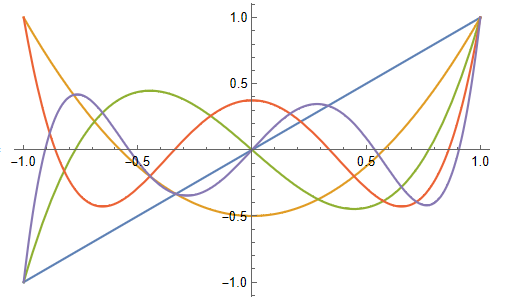
\includegraphics[scale=1]{Captura de pantalla 2023-05-23 032130.png}
    \caption{Polinomios de Legendre normalizados}
    \label{legendre}
\end{figure}
 \end{obs}
 \begin{ejem}[\textbf{Cuadratura de Gauss-Legendre de dos puntos}]
Utilizando la fórmula de recurrencia calculamos $p_2(x)$:
$$p_o=1$$
$$p_1=(x-\alpha_1)p_o$$
$$\alpha_1=\dfrac{\int_{-1}^1xdx}{\int_{-1}^1 dx}=0\Rightarrow p_1=x$$
$$p_2=(x+\alpha_2)p_1-\gamma_2^2p_o$$
$$\gamma_2^2=\dfrac{\int_{-1}^1x^2dx}{\int_{-1}^1 dx}=\dfrac{1}{3}\qquad \alpha_2=\dfrac{\int_{-1}^1x^3dx}{\int_{-1}^1x^2dx}=0\Rightarrow p_2=x^2-\dfrac{1}{3}$$
Los nodos de la cuadratura serán por tanto $x_1=\dfrac{1}{\sqrt{3}}$ y $x_2=-\dfrac{1}{\sqrt{3}}$. Calculemos ahora los pesos de la cuadratura utilizando (\ref{pesos:gauss}):
$$\omega_1=\dfrac{\int_{-1}^1p_1^2dx}{p_1(x_1)p'_2(x_1)}=\dfrac{\frac{2}{3}}{\frac{1}{\sqrt{3}}\cdot \frac{2}{\sqrt{3}}}=1$$
$$\omega_2=\dfrac{\int_{-1}^1p_1^2dx}{p_1(x_2)p'_2(x_2)}=\dfrac{\frac{2}{3}}{\frac{-1}{\sqrt{3}}\cdot \frac{-2}{\sqrt{3}}}=1$$
Obteniendo por tanto la fórmula
\begin{align}
\int_{-1}^1f(x)dx\approx f\left(\dfrac{1}{\sqrt{3}}\right)+f\left(-\dfrac{1}{\sqrt{3}}\right)
\label{legendre:2}
\end{align}
que será exacta para polinomios de grado menor o igual que $3$ (tan exacta como la fórmula de Simpson).
\end{ejem}
\begin{ejem}[\textbf{Cuadratura de Gauss-Legendre de tres puntos}]
Para $n=3$ los nodos de cuadratura serán las raíces de $p_3$
$$p_3(x)=(x-\alpha_3)p_2(x)-\gamma_3^2p_1(x)$$
donde
$$\alpha_3=\dfrac{g_{\omega}(p_2,xp_2)}{g_{\omega}(p_2,p_2)}=-\dfrac{\displaystyle\int_{-1}^1p_2(x)^2\cdot x dx}{\displaystyle\int_{-1}^1p_2(x)^2dx}$$
observemos que
$$\int_{-1}^1p_2(x)\cdot p_2(x)\cdot xdx=\int_{-1}^1p_2(x)\left(x^2-\dfrac{1}{3}\right)x=\int_{-1}^1p_2(x)\cdot x^3dx=0$$
dado que el grado del polinomio del integrando es impar, con lo cual $\alpha_3=0$. Por otro lado:
$$\gamma_3^2=\dfrac{\displaystyle\int_{-1}^1p_2(x)^2dx}{\displaystyle\int_{-1}^1p_1(x)^2dx}=\dfrac{\displaystyle \int_{-1}^1\left(x^2-\dfrac{1}{3}\right)x^2dx}{\frac{2}{3}}=\dfrac{\nicefrac{2}{5}-\nicefrac{2}{9}}{\nicefrac{2}{3}}=\dfrac{4}{15}$$
Concluyendo entonces que
$$p_3(x)=xp_2-\dfrac{4}{15}p_1=x\left(x^2\left(\dfrac{1}{3}+\dfrac{4}{15}\right)\right)=x\left(x^2-\dfrac{3}{5}\right)$$
Y por tanto los nodos de integración serán $x_1=-\sqrt{\dfrac{3}{5}},\,x_2=0\, ,x_3=\sqrt{\dfrac{3}{5}}$. Calculemos ahora los pesos resolviendo el siguiente sistema:
$$\omega_1+\omega_2+\omega_3=g_{\omega}(p_o,p_o)=2$$
$$\omega_1p_1(x_1)+\omega_2p_1(x_2)+\omega_3p_1(x_3)=0$$
$$\omega_1p_2(x_1)+\omega_2p_2(x_2)+\omega_3)p_2(x_3)=0$$
Sustituyendo $x_1=-x_3$ en la primera ecuación obtenemos
$$\omega_2=2-2\omega_1$$
Como $p_1(x)=x$ y $x_1=-x_3$ por la segunda ecuación tenemos que 
$$\omega_1x_1-\omega_3x_1=0\Rightarrow\omega_1=\omega_3$$
Usando esto en la tercera ecuación y dando valores a los nodos tenemos que
$$2\omega_1\left(\dfrac{3}{5}-\dfrac{1}{3}\right)+\omega_2\left(-\dfrac{1}{3}\right)=0$$
$$2\omega_1\left(\dfrac{4}{15}\right)+(2-2\omega_1)\left(-\dfrac{1}{3}\right)=0$$
$$\dfrac{18}{15}\omega_1=\dfrac{2}{3}$$
Despejando obtenemos que $\omega_1=\omega_3=\dfrac{5}{9}$ y con lo cual $\omega_2=\dfrac{8}{9}$, obteniendo por tanto la fórmula
\begin{align}
 \int_{-1}^1f(x)dx\approx\dfrac{5}{9}\cdot f\left(\sqrt{\dfrac{3}{5}}\right)+ \dfrac{8}{9}\cdot f(0)+\dfrac{5}{9}\cdot f\left(\sqrt{\dfrac{3}{5}}\right) 
 \label{legendre:3}
\end{align}

\end{ejem}

\subsection{Fórmula de cuadratura de Gauss-Chebyshev}
\begin{defin}
Las \textbf{cuadraturas de Gauss-Chebyshev} son formas de cuadratura gaussiana con $[a,b]=[-1,1]$ y $\omega(x)=\dfrac{1}{\sqrt{1-x^2}}$. Esto es, fórmulas para aproximar integrales de la forma
$$\int_{-1}^1\dfrac{f(x)}{\sqrt{1-x^2}}dx$$
\end{defin}
\begin{obs}
Haciendo el cambio de variable $x=\cos\theta$ obtenemos lo siguiente
$$\int_{-1}^1\dfrac{f(x)}{\sqrt{1-x^2}}dx=-\int_{\pi}^0f(\cos\theta)\cdot \dfrac{\sin\theta}{\sqrt{1-\cos^2\theta}}d\theta=\int_0^\pi f(\cos\theta)d\theta$$  
\end{obs}
\begin{lem}
Los polinomios de Chebyshev $T_n$ son ortogonales para la norma
$$g_{\omega}(p,q)=\int_{-1}^1\dfrac{p(x)q(x)}{\sqrt{1-x^2}}dx$$
\end{lem}
\begin{dem}
Como $T_i(x)=\cos(i\cdot \arccos(x))$ se tiene que
$$g_{\omega}(T_i,T_j)=\int_{-1}^1\dfrac{T_i(x)T_j(x)}{\sqrt{1-x^2}}=\int_0^{\pi}\cos(i\theta)\cos(j\theta)d\theta$$
Si sumamos las dos siguientes identidades
$$\cos(i\theta+j\theta)=\cos(i\theta)\cos(j\theta)-\sin(i\theta)\sin(j\theta)$$
$$\cos(i\theta-j\theta)=\cos(i\theta)\cos(j\theta)+\sin(i\theta)\sin(j\theta)$$
obtenemos que
$$\cos(i\theta)\cos(j\theta)=\dfrac{\cos(i\theta+j\theta)+\cos(i\theta-j\theta)}{2}$$
Sustituyendo esto en la integral obtenemos lo siguiente:
$$g_\omega(T_i,T_j)=\dfrac{1}{2}\int_0^{\pi}\cos((i+j)\theta)+\dfrac{1}{2}\int_0^{\pi}\cos((i-j)\theta)=0$$
siempre que $i\neq j$.
\qed\end{dem}
\begin{cor}
Los nodos de la cuadratura serán por tanto los nodos de Chebyshev
$$x_k=\cos\left(\dfrac{2k-1}{2n}\pi\right)$$
con $k=1,\ldots,n$
\end{cor}
\begin{prop}[\textbf{Fórmula de cuadratura de Gauss-Chebyshev}] Si $x_i$ son los nodos de Chebyshev, la fórmula
\begin{align}
 \int_{-1}^1\dfrac{f(x)}{\sqrt{1-x^2}}dx\approx\dfrac{\pi}{n}\sum_{i=1}^nf(x_i)
 \label{gauss:cheb}
\end{align}
es exacta para los polinomios de grado menor o igual que $2n-1$.
\end{prop}
\begin{dem}
Sabemos que para que la cuadratura
$$\int_{-1}^1\dfrac{f(x)}{\sqrt{1-x^2}}dx\approx\sum_{i=1}^n\omega_if(x_i) $$
sea exacta para polinomios de grado menor o igual que $2n-1$ los nodos de la cuadratura tienen que ser los nodos de Chebyshev. Para calcular los pesos con la fórmula (\ref{pesos:gauss}) debemos tener en cuenta que los polinomios $T_n(x)$ no son mónicos, esto es, $p_n=2^{1-n}\cdot T_n$. De esta forma:
$$\omega_i=\dfrac{g_\omega(2^{2-n}\cdot T_{n-1},2^{2-n}\cdot T_{n-1})}{2^{1-n}\cdot T'_n(x_i)\cdot 2^{2-n}T_{n-1}(x_i)}=\dfrac{2^{4-2n}}{2^{3-2n}}\cdot \dfrac{g_\omega(T_{n-1},T_{n-1})}{T'_n(x_i)\cdot T_{n-1}(x_i)}= 2\cdot  \dfrac{g_\omega(T_{n-1},T_{n-1})}{T'_n(x_i)\cdot T_{n-1}(x_i)}  $$
Calculemos entonces $\dfrac{dT_n(x)}{dx}$, tomando $x=\cos\theta$
$$\dfrac{dT_n(x)}{dx}=\dfrac{dT_n(\theta)}{d\theta}\cdot \dfrac{d\theta}{dx}=\dfrac{d}{d\theta}(\cos(n\theta))\cdot\dfrac{-1}{\sqrt{1-\cos^2\theta}}=\dfrac{n\sin(n\theta)}{\sin\theta}$$
Con lo cual
$$T'_{n}(x_i)\cdot T_{n-1}(x_i)=\dfrac{n\sin\left(n\cdot\dfrac{2i-1}{2n}\pi\right)}{\sin\left(\dfrac{2i-1}{2n}\pi\right)}\cdot \cos\left(((n-1)\dfrac{2i-1}{2n}\pi\right)=$$
$$=\dfrac{n\sin\left(\dfrac{2i-1}{2}\pi\right)}{\sin\left(\dfrac{2i-1}{2n}\pi\right)}\cdot\left(\cos\left(\dfrac{2i-1}{2}\pi\right)\cdot \cos\left(-\dfrac{2i-1}{2n}\pi\right)+\sin\left(\dfrac{2i-1}{2}\pi\right)\cdot \sin\left(\dfrac{2i-1}{2n}\pi\right)\right)=$$
$$=\dfrac{n\sin\left(\dfrac{2i-1}{2}\pi\right)}{\sin\left(\dfrac{2i-1}{2n}\pi\right)}\cdot\left(\cos\left(i\pi-\dfrac{\pi}{2}\right)\cdot \cos\left(-\dfrac{2i-1}{2n}\pi\right)+\sin\left(\dfrac{2i-1}{2}\pi\right)\cdot \sin\left(\dfrac{2i-1}{2n}\pi\right)\right)=$$
$$=\dfrac{n\sin\left(\dfrac{2i-1}{2}\pi\right)}{\sin\left(\dfrac{2i-1}{2n}\pi\right)}\cdot\left(\sin\left(i\pi\right)\cdot \cos\left(-\dfrac{2i-1}{2n}\pi\right)+\sin\left(\dfrac{2i-1}{2}\pi\right)\cdot \sin\left(\dfrac{2i-1}{2n}\pi\right)\right)=$$
$$=n\cdot \sin^2\left(\dfrac{2i-1}{2}\pi\right)=n$$
Calculemos ahora el numerador:
$$g_{\omega}(T_{n-1},T_{n-1})=\int_{-1}^1\dfrac{T_{n-1}(x)^2}{\sqrt{1-x^2}}dx=\int_{-1}^1\cos^2((n-1)\theta)=\int_{-1}^1\dfrac{1+\cos(2(n-1)\theta)}{2}=\dfrac{\pi}{2}$$
Reuniendo los resultados anteriores, podemos concluir que
$$\omega_i=\dfrac{\pi}{n}$$
\qed\end{dem}
\subsection{Error de las cuadraturas gaussianas}
\begin{prop}
El error de la fórmula de cuadratura gaussiana
$$\int_a^bf(x)\omega(x)dx\approx\sum_{i=1}^n\omega_if(x_i)$$
viene dado por la expresión
\begin{align}
 \mathcal{E}_G=\dfrac{f^{(2n)}(\xi)}{(2n)!}g_{\omega}(p_n,p_n)
 \label{error:gauss}
\end{align}
\end{prop}
\begin{dem}
 Como siempre, tenemos que calcular
 $$\mathcal{E}=\int_a^bf(x)\omega(x)dx-\sum_{i=1}^n\omega_if(x_i)$$
 Sea ahora $H(x)$ el polinomio de interpolación de Hermite de $f(x)$ correspondiente a los pares $\{(x_1,\alpha_1),\ldots,(x_n,\alpha_n)\}$. Queremos que el grado del polinomio sea máximo, esto es, de grado $2n-1$, con lo cual:
 $$\sum_{i=1}^n\alpha_1+n-1=2n-1\Longrightarrow\sum_{i=1}^n\alpha_i=n$$
 Luego tomando $\alpha_i=1$ tenemos que $H(x)$ es de grado $2n-1$. De esta forma:
 $$\int_a^bf(x)\omega(x)dx-\sum_{i=1}^n\omega_if(x_i)=\int_a^bf(x)\omega(x)dx-\sum_{i=1}^n\omega_iH(x_i)=
 \int_a^bf(x)\omega(x)dx-\int_{a}^bH(x)\omega(x)dx=$$
 $$=\int_a^b(f(x)-H(x))\omega(x)dx$$
 Y por la fórmula del error de la interpolación de Hermite (\ref{error:herm})
 $$\mathcal{E}=\int_a^b\dfrac{f^{(2n)}(\xi)}{(2n)!}\prod_{i=1}^n(x-x_i)^2\omega(x)dx=$$
 $$=\dfrac{f^{(2n)}(\xi)}{(2n)!}\int_a^b\prod_{i=1}^n(x-x_i)^2\omega(x)dx=\dfrac{f^{(2n)}(\xi)}{(2n)!}g_{\omega}(p_n,p_n)$$
 donde hemos empleado que $p_n(x)=\prod_{i=1}^n(x-x_i)$ por ser una cuadratura gaussiana.
\qed\end{dem}
\subsection{Cálculo efectivo de los nodos y los pesos}
\begin{obs}
Los métodos numéricos para calcular los autovalores de matrices son más estables que los que calculan las raíces de polinomios. Por esta razón, desarrollaremos un método matricial para calcular los nodos y los pesos de las cuadraturas gaussianas.
\end{obs}
\begin{met}[\textbf{de Golub-Welsch}]
Si $p_o,\ldots,p_n$ son los polinomios ortogonales de la cuadratura, sabemos que están relacionados por la fórmula
$$p_{i+1}=(x-\alpha_{i+1})p_i(x)-\gamma_{i+1}^2p_{i+1}(x)$$
de esta forma
$$xp_i(x)=\gamma_{i+1}^2p_{i-1}+\alpha_ip_i(x)+p_{i+1}$$
luego si $x_i$ son los nodos de la cuadratura
$$x_i\cdot\left(\begin{array}{c}
     p_o(x_i) \\
      p_1(x_i)\\
      \vdots\\
      p_{n-1}
\end{array}\right)=\left(\begin{array}{cccc}
     \alpha_1&1&\cdots&0 \\
      \gamma_2^2&\alpha_2&\ddots&\vdots\\
      \vdots&\ddots&\ddots&1\\
      0&\cdots&\gamma_n^2&\alpha_n
\end{array}\right)\cdot \left(\begin{array}{c}
     p_o(x_i) \\
      p_1(x_i)\\
      \vdots\\
      p_{n-1}(x_i)
\end{array}\right) $$
Si tomamos
$$e=\left(\begin{array}{c}
     p_o(x_i) \\
      p_1(x_i)\\
      \vdots\\
      p_{n-1}(x_i)
\end{array}\right)\qquad \tilde{J}_n=\left(\begin{array}{cccc}
     \alpha_1&1&\cdots&0 \\
      \gamma_2^2&\alpha_2&\ddots&\vdots\\
      \vdots&\ddots&\ddots&1\\
      0&\cdots&\gamma_n^2&\alpha_n
\end{array}\right)$$
tenemos que $\tilde{J}_n e=x_i\cdot e$, esto es, $e$ es un valor propio de $\tilde{J}_n$ de valor propio $x_i$. Vamos a hacer un cambio de base diagonal de tal forma que la matriz de $\tilde{J}_n$ sea simétrica, esto es
$$J_n=D^{-1}\cdot \tilde{J}_n\cdot D$$
$$D=\left(\begin{array}{cccc}
     \lambda_1&0&\cdots&0 \\
      0&\lambda_2&\ddots&\vdots\\
      \vdots&\ddots&\ddots&0\\
      0&\cdots&0&\lambda_n
\end{array}\right)\qquad J_n=\left(\begin{array}{cccc}
     \alpha_1&\gamma_2&\cdots&0 \\
      \gamma_2&\alpha_2&\ddots&\vdots\\
      \vdots&\ddots&\ddots&\gamma_n\\
      0&\cdots&\gamma_n&\alpha_n
\end{array}\right)$$
Queremos entonces que se verifique que $$(\tilde{J}_n\cdot D )e_i=(D\cdot J_n)e_i$$ para todos los vectores $e_i$ de la base estándar de $\mathbb{R}^n$. Por un lado tenemos que
$$(D\cdot J_n)e_i=D(\gamma_{i-1}+\alpha_ie_i+\alpha_{i+1}e_{i+1})=\lambda_{i-1}\gamma_i e_{i-1}+\lambda_i\alpha_i e_i+\lambda_{i+1}\gamma_{i+1} e_{i+1}$$
y por otro que
$$(\tilde{J}_n\cdot D )e_i=\tilde{J}_n(\lambda_ie_i)=\lambda_i e_{i-1}+\lambda_i\alpha_i e_i+\lambda_i\gamma_{i+1}^2 e_{i+1}$$
Si igualamos los coeficientes podemos concluir que
$$\lambda_i= \gamma_i\cdot \lambda_{i-1}=\gamma_{i}\cdot \gamma_{i-1}\cdot\lambda_{i-2}=\cdots=\gamma_2\cdot \ldots \cdot \gamma_i\cdot \lambda_1$$
donde tomaremos $\lambda_1=1$ por ser arbitrario. Reuniendo estos resultados deducimos que los vectores
$$\tilde{v}^{(i)}=D^{-1} e= \left(\begin{array}{c}
     \nicefrac{1}{\lambda_1}\cdot p_o(x_i) \\
     \nicefrac{1}{\lambda_2}\cdot p_1(x_i)\\
      \vdots\\
     \nicefrac{1}{\lambda_n}\cdot p_{n-1}(x_i)
\end{array}\right)\qquad \lambda_i= \gamma_2\cdot \ldots \cdot \gamma_i$$
son vectores propios de $J_n$ de valor propio $x_i$ ya que
$$J_n(D^{-1}e)=(D^{-1}\cdot \tilde{J}_n\cdot D)(D^{-1}e)=D^{-1}\cdot \tilde{J}_n e=D^{-1}(x_i\cdot e)=x_i\cdot (D^{-1}e)$$
Podemos emplear lo deducido anteriormente para calcular los pesos de las cuadraturas gaussianas como sigue. El sistema que determina los nodos se escribe en la base $\tilde{v}^{(i)}$ como
$$\sum_{i=1}^n \rho_j\cdot p_o(x_i)\omega_i=\left\{ 
\begin{array}{cc}
   g_{\omega}(p_o,p_o)   &  j=0 \\
    0 & j\neq 0 
\end{array}\right.  $$
 con $\rho_o=1$ y $\rho_j=\dfrac{1}{\lambda_{j+1}}$. Si lo escribimos de forma matricial
 $$\left(\begin{array}{c|c|c|c}
      \tilde{v}^{(1)} & \tilde{v}^{(2)} &\cdots & \tilde{v}^{(n)} 
 \end{array}\right)\cdot \left(\begin{array}{c}
     \omega_1 \\
      \omega_2\\
      \vdots\\
      \omega_n
\end{array}\right)=\left(\begin{array}{c}
     g_{\omega}(p_o,p_o) \\
     0\\
      \vdots\\
      0
\end{array}\right) $$
Por ser $J_n$ simétrica y los $x_i$ distintos, sabemos que los $\tilde{v}^{(i)}$ son ortogonales entre sí, esto es, $(\tilde{v}^{(j)})^t\cdot\tilde{v}^{(i)}=\delta_{ij}\cdot \|\tilde{v}^{(i)}\|^2 $. Multiplicando el sistema anterior por $(\tilde{v}^{(i)})^t$ tenemos que
 $$\left(\begin{array}{c|c|c|c}
     )\tilde{v}^{(i)})^t\cdot  \tilde{v}^{(1)} &(\tilde{v}^{(i)})^t\cdot  \tilde{v}^{(2)} &\cdots &(\tilde{v}^{(i)} )^t\cdot \tilde{v}^{(n)} 
 \end{array}\right)\cdot \left(\begin{array}{c}
     \omega_1 \\
      \omega_2\\
      \vdots\\
      \omega_n
\end{array}\right)=(\tilde{v}^{(i)})^t\cdot \left(\begin{array}{c}
     g_{\omega}(p_o,p_o) \\
     0\\
      \vdots\\
      0
\end{array}\right) $$
 $$\left(\begin{array}{c|c|c|c|c}
     0 &\cdots  &\|\tilde{v}^{(i)}\|^2&\cdots&0 
 \end{array}\right)\cdot \left(\begin{array}{c}
     \omega_1 \\
      \omega_2\\
      \vdots\\
      \omega_n
\end{array}\right)=\tilde{v}_1^{(i)}\cdot g_{\omega}(p_o,p_o)
$$
Como $\tilde{v}_1^{(i)}=\dfrac{1}{\lambda_1}\cdot p_o(x_i)=1$, podemos concluir que
$$\omega_i=\dfrac{g_{\omega}(p_o,p_o)}{\|\tilde{v}^{(i)}\|^2}$$
Supongamos ahora que $v^{(i)}$ es otro vector propio  de valor propio $x_i$. Se tiene entonces que
$$v^{(i)}=\mu\cdot \tilde{v}^{(i)}\Rightarrow \|v^{(i)}\|^2=\mu^2\cdot \|\tilde{v}^{(i)}\|^2\Rightarrow \|\tilde{v}^{(i)}\|^2=\dfrac{\|v^{(i)}\|^2}{\mu^2}$$
Sustituyendo esto en la fórmula anterior
$$\omega_i=\dfrac{g_{\omega}(p_o,p_o)}{\|v^{(i)}\|^2}\cdot \mu^2$$
y como $\tilde{v}_1^{(i)}=1$, $\mu=v_1^{i}$. Con este resultado obtenemos el siguiente teorema.
\end{met}
\begin{teo}
Sea $v^{(i)}$ un vector propio de $J_n$ con valor propio $x_i$ y tal que $\|v^{(i)}\|^2=g_{\omega}(p_o,p_o)$. Entonces, los pesos de la cuadratura gaussiana son
$$\omega_i=(v_1^{(i)})^2$$
\end{teo}
\section{Ejercicios}
\begin{ejer}
Calcula $\ln(2)$ con un error menor que $0.01$ utilizando el método de Simpson compuesto aplicado a la integral
$$\ln(2)=\int_1^2\dfrac{1}{x}dx$$
\end{ejer}
\begin{sol}
Calculemos en primer lugar el número de subvintervalos necesarios para que el error sea menor que $0.001$ utilizando la fórmula del error del método de Simpson compuesto:
$$\dfrac{M_4}{180}\cdot(b-a)\cdot \left(\dfrac{b-a}{2n}\right)^4<0.01$$
donde $M_4=\max|f^{(4)}|$ con $x\in[1,2]$ y $f(x)=\dfrac{1}{x}$. Acotemos por tanto  $f^{(4)}(x)$:
$$f'(x)=-\dfrac{1}{x^2}$$
$$f''(x)=\dfrac{2}{x^3}$$
$$f^{(3)}(x)=-\dfrac{6}{x^4}$$
$$f^{(4)}(x)=\dfrac{24}{x^5}$$
$$f^{(5)}(x)=-\dfrac{120}{x^6}$$
Como $f^{(5)}(x)<0$ y nunca se anula, el máximo de $f^{(4)}(x)$ ocurre en $x=1$, esto es $M_4=|f^{(4)}(1)|=24$. Calculemos a continuación la $n$:
$$\dfrac{24}{180}\cdot(2-1)\cdot \left(\dfrac{2-1}{2n}\right)^4<0.001$$
$$\dfrac{1}{n^4}<0.12$$
$$n>1.7$$
Luego tomaremos $n=2$. Aplicando la fórmula de Simpson compuesta con $h_n=\dfrac{1}{4}$ obtenemos lo siguiente
$$\int_1^2\dfrac{1}{x}dx\approx \dfrac{1}{12}(f(1)+2f(1.5)+4(f(1.25)+f(1.75))+f(2))\approx 0.69325$$
siendo el valor ''real'' de $\ln(2)=0.69314\ldots$
\end{sol}
\begin{ejer}
    Una cuerda vibra adoptando la forma $y=\sin x $, entre las abcisas $x=0$ y $x=4$ en un instante $t_o$. Calcúlese aproximadamente la longitud de la cuerda, utilizando un método numérico con $n=8$. Acotar el error cometido.
\end{ejer}
\begin{sol}
Sabemos que la longitud de la cuerda se puede calcular mediante la integral
$$L=\int_0^4\sqrt{1+(y')^2}=\int_0^4\sqrt{1+\cos^2x}dx$$
Empleemos la fórmula del trapecio compuesto con $n=8$ para aproximar dicha integral. Tendremos entonces que $h_n=\dfrac{4-0}{8}=0.5$ y el integrando será $g(x)=\sqrt{1+\cos^2x}$. Necesitaremos por tanto los siguientes datos:
$$\begin{array}{|c|c|c|c|c|c|c|c|c|}
    \hline
     x_o&x_1&x_2&x_3&x_4&x_5&x_6&x_7&x_8  \\
     0.0&0.5&1.0&1.5&2.0&2.5&3.0&3.5&4.0 \\
     \hline
     g(x_o)&g(x_1)&g(x_2)&g(x_3)&g(x_4)&g(x_5)&g(x_6)&g(x_7)&g(x_8)\\
     1.41421&1.33047&1.13663&1.0025&1.08313&1.28134&1.40715&1.37002&1.18468\\
     \hline
\end{array}$$
Con lo cual:
$$L\approx \dfrac{1}{6}\left(g(x_o)+2\sum_{i=1}^7g(x_i)+g(x_8)\right)\approx 4.9578$$
Analicemos ahora el error de este método:
$$\mathcal{E}\leq \dfrac{M_2}{12}\cdot (b-a)\cdot h_n^2=\dfrac{M_2}{12}\cdot 4\cdot\dfrac{1}{4}=\dfrac{M_2}{12}$$
donde $M_2=\max|g''(x)|$ con $x\in[0,4]$. Acotemos por tanto $g''(x)$:
$$|g''(x)|=\left|\dfrac{\cos(2x)+\cos^4x}{(1+\cos^2x)^{\frac{3}{2}}}\right|\leq \left|\dfrac{1}{(1+\cos^2x)^{\frac{3}{2}}}\right| \cdot (|\cos(2x)|+|\cos^4x|)\leq 1\cdot (1+1)=2 $$
Y con lo cual $M_2\leq 2$, de esta forma:
$$\mathcal{E}\leq\dfrac{2}{12}\approx 0.167$$
\end{sol}
\begin{ejer}
Se desea evaluar la integral
$$I=\int_0^1e^{-x^2}dx$$
por un método de integración numérica con un error menor a $10^{-5}$. Determina el número de subintervalos a considerar en los métodos del trapecio y de Simpson para conseguir dicha precisión.
\end{ejer}
\begin{sol}
Estudiemos en primer luegar el número de subintervalos necesarios para el método del trapecio. Empleando la fórmula del error para este método, sabemos que se debe verificar que
$$\dfrac{M_2}{12}\cdot(b-a)\cdot\left(\dfrac{b-a}{n}\right)^2<10^{-5}$$
$$\dfrac{M_2}{12}\cdot\dfrac{1}{n^2}<10^{-5}$$
$$n>\sqrt{\dfrac{10^{5}\cdot M_2}{12}}$$
donde $M_2=\max|f''(x)|$ con $x\in[0,1]$ y $f(x)=e^{-x^2}$. Calculemos entonces las primeras derivadas de $f(x)$:
$$f'(x)=-2x\cdot e^{-x^2}$$
$$f''(x)=(4x^2-2)e^{-x^2}$$
$$f^{(3)}(x)=-4x(2x^2-3)\cdot e^{-x^2}$$
Como $f^{(3)}(x)$ se anula en $x_1=0$ y en $x_2=\sqrt{\dfrac{3}{2}}$ pero $x_2\nin [0,1]$, los posibles máximos de $|f''(x)|$ son los extremos del intervalo:
$$|f''(0)|=|-2|=2$$
$$|f''(1)|=\dfrac{2}{e}<2$$
Por tanto, $M_2=2$ y se tiene entonces que
$$n>\sqrt{\dfrac{10^{5}\cdot 2}{12}}\approx 129.099$$
Luego para emplear el método del trapecio compuesto necesitaríamos al menos 130 subintervalos.

Analicemos ahora el método de Simpson. Empleando la fórmula del error podemos deducir que
$$\dfrac{M_4}{180}\cdot (b-a)\cdot \left(\dfrac{b-a}{2n}\right)^4<10^{-5}$$
$$\dfrac{M_4}{180}\cdot\dfrac{1}{16n^4}$$
$$n>\sqrt[4]{\dfrac{10^5\cdot M_4}{2880}}$$
donde $M_4=\max|f^{(4)}|$. Acotemos por tanto $|f^{(4)}(x)|$:
$$f^{(4)}(x)=4(4x^4-12x^2+3)\cdot e^{-x^2}$$
$$f^{(5)}(x)=-8x(4x^{4}-20x^2+15)\cdot e^{-x^2}$$
Resolviendo $f^{(5)}(x)=0$ obtenemos los posibles máximos de $|f^{(4)}(x)|$. Además de la solución $x=0$, debemos considerar las soluciones de 
$$4x^4-20x^2+15=0$$
que serán
$$x_1=-\sqrt{\dfrac{5}{2}-\sqrt{\dfrac{5}{2}}} \qquad x_2=\sqrt{\dfrac{5}{2}-\sqrt{\dfrac{5}{2}}} $$
$$x_3=-\sqrt{\dfrac{5}{2}+\sqrt{\dfrac{5}{2}}} \qquad x_4=\sqrt{\dfrac{5}{2}+\sqrt{\dfrac{5}{2}}} $$
Como $x_1,x_3,x_4\nin [0,1]$, debemos considerar los siguientes casos:
$$|f^{(4)}(0)|=12$$
$$|f^{(4)}(x_2)|\approx 7.4194$$
$$|f^{(4)}(1)|\approx 7.3575$$
Y por tanto $M_2=12$, de esta forma
$$n>\sqrt[4]{\dfrac{10^5\cdot 12}{2880}}\approx 4.5180$$
Esto es, necesitaríamos por lo menos $5$ subintervalos para alcanzar la precisión requerida.
\end{sol}
\begin{ejer}
Calcula la integral del problema anterior usando una cuadratura de Gauss con $n=3$. Sabiendo que el resultado ''exacto'' es $I=0.7468241330\ldots$, compara los resultados
\end{ejer}
\begin{sol}
Para emplear la cuadratura de Gaus-Legendre de tres puntos debemos estar trabajando en el intervalo de integración $[-1,1]$. Haciendo el siguiente cambio de variable
$$x=\dfrac{1}{2}-\dfrac{t}{2}$$
$$dx=-\dfrac{1}{2}dt$$
Obtenemos lo siguiente:
$$\int_0^1e^{-x^2}=\int_1^{-1}e^{-\frac{1}{4}(t-1)^2}\cdot \dfrac{-1}{2}dt=\dfrac{1}{2}\int_{-1}^1e^{-\frac{1}{4}(t-1)^2}$$
Si denotamos por $f(t)=e^{-\frac{1}{4}(t-1)^2}$, aplicando la cuadratura de Gauss-Legendre tenemos que
$$I\approx \dfrac{5}{18}\cdot f\left(\sqrt{\dfrac{3}{5}}\right)+ \dfrac{8}{18}\cdot f(0)+\dfrac{5}{18}\cdot f\left(\sqrt{\dfrac{3}{5}}\right)\approx 0.78157$$
Es decir, hemos obtenido un error de menor que $0.1$.
\end{sol}
\begin{ejer}
Calcula la integral
$$I=\int_{-1}^1\dfrac{e^x}{\sqrt{1-x^2}}dx$$
utilizando las cuadraturas de Gauss-Chebyshev correspondientes a $n=2$ y $n=3$. Evalúa el error en ambos casos sabiendo que el resultado ''exacto'' de la integral es $I=3.9774632...$
\end{ejer}
\begin{sol}
Para $n=2$ los nodos de Chebyshev son
$$x_1=\cos\left(\dfrac{\pi}{4}\right)\qquad x_2=\cos\left(\dfrac{3\pi}{4}\right)$$
Por tanto, tomando $f(x)=e^x$ la aproximación obtenida con la cuadratura de Gauss-Chebyshev será
$$I\approx \dfrac{\pi}{2}\left(f\left(\cos\left(\dfrac{\pi}{4}\right)\right)+f\left(\cos\left(\dfrac{3\pi}{4}\right)\right)\right)\approx 3.96027$$
Teniendo por tanto un error menor que $0.1$.

Por otro lado, para $n=3$ los nodos de Chebyshev son
$$x_1=\cos\left(\dfrac{\pi}{6}\right)\qquad x_2=0 \qquad x_3=\cos\left(\dfrac{5\pi}{6}\right)$$
Y la aproximación que obtenemos con la cuadratura de Gauss-Chebyshev es
$$I\approx \dfrac{\pi}{3}\left(f\left(\cos\left(\dfrac{\pi}{6}\right)\right)+f(0)+f\left(\cos\left(\dfrac{5\pi}{6}\right)\right)\right)\approx 3.97732$$
Obteniendo un error menor que $0.001$.
\end{sol}





























































\begin{comment}
 
    Consiste en encontrar f{\'o}rmulas (de cuadratura) de la forma:
    $$\int_a^b f(x) \: dx \approx \sum_{i=0}^n \omega_i \: f(x_i)$$
    donde llamaremos a los $\omega_i$ pesos y a los $x_i$ nodos. 
        \subsection{F{\'o}rmulas de integraci{\'o}n interpolatorias}
        \begin{enumerate}[a)]
            \item Los nodos est{\'a}n prefijados: $x_o=a, \ldots, x_k = a + kh_1, \ldots, x_n=b$ con $h=\dfrac{b-a}{n}$ \\
            \textbf{Ejemplo.} F{\'o}rmulas de Newton-Cotes: hay que calcular los $n+1$ pesos $\omega_i$. Para $n=1$ es la f{\'o}rmula del trapecio (se ven ambas m{\'a}s adelante). 
            \item Calcular los nodos y los pesos para que la precisi{\'o}n sea la mayor posible. Se aproxima $f(x)$ por un polinomio de interpolaci{\'o}n de grado $n$. \\
            
        \end{enumerate}
        \subsection{F{\'o}rmula del error} Como siempre, el error es $$\mc{E}(f)=\int_a^b f(x) \: dx - \sum_{i=0}^n \omega_i \: f(x_i)=\int_a^b f(x) \: dx - \int_a^b p_n(x) dx = \int_a^b (f(x)-p_n(x)) \: dx $$
        $$\mc{E}(f)=\int_a^b \dfrac{f^{(n+1)}(\xi)}{(n+1)!} \prod_{i=0}^n (x-x_i) \: dx$$
        \subsection{F{\'o}rmulas de Newton-Cotes}
        Son las fórmulas de cuadratura obtenidas por la integración de $p_n(x)$ polinomio de interpolación de $f$ en $\{x_o, \ldots, x_n\}$ con $x_i = a + i \: \dfrac{b-a}{n}$. Es decir, $\displaystyle \omega_i = \int_a^b \ell_i (x) \: dx$, y por tanto $\displaystyle \int_a^b p_n(x)\:dx = \sum_{i=0}^n \omega_i \: p_n(x_i)$. Para $n=1$ se tiene
        \subsection{F{\'o}rmula del trapecio}
        Tomemos como intervalo de referencia [-1,1], entonces
        $$\int_{-1}^1 f(t) \: dt \approx \omega_o f(-1) + \omega_1 \: f(1)$$
        Como se ha dicho, 
        $$\omega_o=\int_{-1}^1 \ell_o(t) \: dt = \int_{-1}^1 \dfrac{t-1}{-1-1} \: dt = - \dfrac{1}{2} \int_{-1}^1 (t-1) \: dt = - \dfrac{1}{2} \dfrac{1}{2} (t-1)^2 \Big|_{-1}^1 = - \dfrac{1}{4} (-4) = 1$$
        $$\omega_1 = \int_{-1}^1 \ell_1(t) \: dt = \int_{-1}^1 \dfrac{t+1}{2} \: dt = \dfrac{1}{4}(t+1)^2 = \dfrac{1}{4} \: 4 = 1$$
        Por tanto, $\displaystyle 2 = \int_{-1}^1 dt = f(-1) + f(1)$ \textcolor{red}{NO ENTIENDO EL 2} \\
        \textbf{Proposici{\'o}n.}
        Si $\displaystyle \sum_{i=0}^{n} \omega_i \: f(x_i)$ es una f{\'o}rmula de cuadratura interpolaria exacta para polinomios de grado $\leq n$, en particular
        $$\sum_{i=0}^n \omega_i = b-a = \int_a^b dx$$
        Ahora, para calcular la f{\'o}rmula en un intervalo [$a,b$] arbitrario, hacemos un cambio de coordenadas $x=\dfrac{a+b}{2}+t\:\dfrac{b-a}{2} \Rightarrow dx=\dfrac{b-a}{2} \: dt$, por tanto,
        $$\int_a^b f(x) \: dx= \int_{-1}^1 f\left(\dfrac{a+b}{2}+t\:\dfrac{b-a}{2}\right)\dfrac{b-a}{2} \: dt = \dfrac{b-a}{2} \int_{-1}^1 f\left(\dfrac{a+b}{2}+t\:\dfrac{b-a}{2}\right) \: dt \approx $$
        $$\approx \dfrac{b-a}{2} (f(a)+f(b))$$
            \subsubsection{F{\'o}rmula del error del trapecio}
            Como siempre, el error viene dado por
            $$\mc{E}_T=\int_a^b f(x) \: dx - \dfrac{b-a}{2} (f(a)+f(b)) = \int_a^b \dfrac{f^{(2)}(\xi)}{2} (x-a)(x-b) \: dx =   \hfill $$
            $$=\dfrac{f^{(2)}(\xi)}{2} \int_a^b\left(\dfrac{a+b}{2}+t\:\dfrac{b-a}{2}-a\right) \left(\dfrac{a+b}{2}+t\:\dfrac{b-a}{2}-b\right)\dfrac{a-b}{2} \: dt =\dfrac{f^{(2)}(\xi)}{2} \left( \dfrac{b-a}{2}\right)^3\int_{-1}^{1}(t+1)(t-1)\:dt= $$
            $$ = \dfrac{f^{(2)}(\xi)}{2} \left( \dfrac{b-a}{2}\right)^3\int_{-1}^{1}(t-1)^2\:dt= \dfrac{f^{(2)}(\xi)}{2} \left( \dfrac{b-a}{2}\right)^3 \left( \dfrac{2}{3} - 2 \right) = -2 \dfrac{f^{(2)}(\xi)}{2} \left( \dfrac{b-a}{2}\right)^3 = - \dfrac{f^{(2)}(\xi)}{12} \left( {b-a}\right)^3$$
        \subsection{F{\'o}rmula de Simpson}
        Si $n=2$, aproximamos $f(x)$ por $p_2(x)$ polinomio de interpolaci{\'o}n de $f$ en $a,\frac{a+b}{2}, b$
        $$\int_a^b f(x) \: dx \approx \omega_o f(a) + \omega_1 f\left(\dfrac{a+b}{2}\right) + \omega_2 f(b)$$
        Como antes, tomamos el intervalo de referencia $[-1,1]$,
        $$\omega_o=\int_{-1}^1 \ell_o(t) \: dt = \int_{-1}^1 \dfrac{t(t-1)}{(-1)(-2)} \:dt =\dfrac{1}{2} \int_{-1}^1 (t^2-t) \: dt = \dfrac{1}{3} \hfill$$
        $$\omega_1=\int_{-1}^1 \ell_1(t) \: dt = \int_{-1}^1 \dfrac{(t+1)(t-1)}{(-1)1} = - \int_{-1}^1 (t^2-1) = \dfrac{4}{3}$$
        $$\omega_2=\int_{-1}^1 \ell_2(t) \: dt = \int_{-1}^1 \dfrac{(t+1)t}{2 \cdot 1} \: dt = \dfrac{1}{3}$$
        Por tanto, $\displaystyle \int_{-1}^1 f(t) \: dt = \dfrac{1}{3} (f(-1)+4f(0)+f(1))$. Procediendo como antes por el cambio de variable:
        $$\int_a^b f(x) \: dx = \int_{-1}^1 f\left(\dfrac{a+b}{2}+t\:\dfrac{b-a}{2}\right)\dfrac{b-a}{2} \: dt = \dfrac{b-a}{2} \int_{-1}^1 f\left(\dfrac{a+b}{2}+t\:\dfrac{b-a}{2}\right) \: dt \approx $$
        $$\approx \dfrac{b-a}{2} \dfrac{1}{3} (f(a)+4f\left(\dfrac{a+b}{2}\right)+f(b)) = \dfrac{b-a}{6} (f(a)+4f\left(\frac{a+b}{2}\right)+f(b)) $$
        \subsubsection{Error}
        Podeos observar que interpola de manera exacta a polinomios de grado $\leq 3$.
        $$\mc{E}_S = - \dfrac{1}{90} (b-a)^5 f^{(4)}(\xi)$$
        
        \textbf{Proposici{\'o}n.} Dado el intervalo $[a,b]$, sean $x_o, \ldots, x_{2k}$ dados por $x_i=a+i\:\dfrac{b-a}{2k}$, se tiene que
        $$\bbint_a^b \prod_{i=0}^{2k} (x-x_i) \: dx = 0$$ 
        \textit{Demostraci{\'o}n.} \textcolor{red}{METER}
        
        \textbf{Corolario.}
        La f{\'o}rmula de Newton-Cotes es exacta para los polinomios de grado menor o igual que $2k+1=n+1$. \\
        \textit{Demostraci{\'o}n.}
        \subsection{F{\'o}rmulas compuestas} Para disminuir el error, lo m{\'a}s pr{\'a}ctico es disminuir el tamaño del intervalo; por ejemplo, dividiendo el intervalo en $n$ partes iguales obteniendo las fórmulas de cuadratura compuestas:
        \begin{itemize}
            \item \underline{Trapecio compuesto:} dado $[a,b]$, sean $\{x_o, \ldots, x_n\}$ los puntos $x_i=0+i\:\dfrac{b-a}{n}$. As{\'i}, $$\int_a^b f(x)\: dx = \sum_{i=0}^{n-1} \int_{x_i}^{x_{i+1}} f(x) \: dx \approx \sum_{i=0}^{n-1} \dfrac{b-a}{2n}(f(x_i)+f(x_{i+1})) = $$
            $$=\dfrac{b-a}{2n} \sum_{i=0}^{n-1} (f(x_i)+f(x_{i+1}))= \dfrac{b-a}{2n} \left( f(a) + 2 \sum_{i=0}^{n-1} f(x_i) + f(b) \right) $$
            Error:
            $$\int_{x_i}^{x_{i+1}} f(x) \: dx - \dfrac{x_{i+1}-x_i}{2}(f(x_i)+f(x_{i+1}))=-\dfrac{f^{(2)}(\xi_i)}{12}(x_{i+1}-x_i)^3= -\dfrac{f^{(2)}(\xi_i)}{12} \left( \dfrac{b-a}{n} \right)^3$$
            Luego 
            $$\int_a^b f(x) \: dx - \dfrac{b-a}{2n} \left( f(a)+2 \sum_{i=0}^{n-1} f(x_i) + f(b) \right) = \sum_{i=0}^{n-1} -\dfrac{f^{(2)}(\xi_i)}{12} \left(\dfrac{b-a}{n}\right)^3=$$
            $$=-\dfrac{1}{12} \left(\dfrac{b-a}{n}\right)^3 \sum_{i=0}^{n-1} f^{(2)}(\xi_i) = -\dfrac{ f^{(2)}(\xi_i)}{12} n \: \left(\dfrac{b-a}{n}\right)^3 =  -\dfrac{f^{(2)}(\xi_i)}{12} n \: \left(b-a\right) h_n^2$$
            donde $h_n = \dfrac{b-a}{n}$
            \item \underline{M{\'e}todo de Simpson compuesto:} dado el intervalo $I=[a,b]$, sean $x_i=a+i\:\dfrac{b-a}{n}$ con $i=0,\ldots, n$
            $$\int_a^b f(x)\: dx = \sum_{i=0}^{n-1} \int_{x_i}^{x_{i+1}} f(x) \:dx \approx \sum_{i=0}^{n-1} \dfrac{1}{6} \dfrac{b-a}{n} \left( f(x_i) + f\left(\dfrac{x_i+x_{i+1}}{2} \right)+ f(x_{i+1})\right)$$
            $$\int_a^b f(x)\: dx \approx \dfrac{b-a}{6n} \left( f(a) + 2 \sum_{i=0}^{n-1} f(x_i) + 4 \sum_{i=0}^{n-1} f\left(\dfrac{x_i+x_{i+1}}{2} \right) + f(b)\right)$$
            Adem{\'a}s, $\dfrac{x_i+x_{i+1}}{2} = \dfrac{1}{2} \left( a+i\:\dfrac{b-a}{n}+a+(i+1)\dfrac{b-a}{n} \right) = a+(2i+1)\dfrac{b-a}{2n}=a+j\:\dfrac{b-a}{2n}$. Si 
            $y_j=a+j\:\dfrac{b-a}{2n}=\left\{ \begin{array}{ll}
               x_i & \text{ si } j=2i (\text{par}) \\
               \dfrac{x_i+x_{i+1}}{2} & \text{ si } j=2i+1 (\text{impar})
            \end{array}\right.$ y la f{\'o}rmula de Simpson compuesta quedar{\'i}a
            $$I \approx \dfrac{1}{3} h_n  \left( f(a) + 2 \sum_{i=0}^{n-1} f(y_{2i}) + 4 \sum_{i=0}^{n} f\left(y_{2i+1} \right) + f(b)\right)$$
            con $h_n=\dfrac{b-a}{2n}$ y $x_i=a+i \: \dfrac{b-a}{3}, \; y_j=a+j\:\dfrac{b-a}{6}=a+j\: h_3$\\
            Error: 
            $$\int_{x_i}^{x_{i+1}} f(x) \: dx - \dfrac{x_{i+1}-x_i}{6} \: \left(f(x_i)+4 f\left(\dfrac{x_i+x_{i+1}}{2}\right) + f(x_{i+1})\right) = - \dfrac{f^{(4)}(\xi_i)}{90} (x_{i+1}-x_i)^5$$
            de manera que sumando todos los errores en cada intervalo, el error total ser{\'a}:
            $$\sum_{i=0}^{n-1} - \dfrac{f^{(4)}(\xi_i)}{90} \left(\dfrac{b-a}{2n}\right)^5 =- \dfrac{f^{(4)}(\xi)}{90} n \: \left(\dfrac{b-a}{2n}\right)^5 = - \dfrac{f^{(4)}(\xi)}{90}\: \left(\dfrac{b-a}{2}\right) \:  h_n^4 = - \dfrac{f^{(4)}(\xi)}{180}\: (b-a) \:  h_n^4$$
        \end{itemize}
        \subsection{Cuadraturas adaptativas}
        Se trata de adoptar los intervalos de integraci{\'o}n en las caracter{\'i}sticas de la funci{\'o}n a integrar. La idea clave es la de estudiar el error cometido comparando dos integrales num{\'e}ricas consecutivas. \\
        Sea $Q$ una f{\'o}rmula de cuadratura tal que 
        $$I = I_1 + I_2 = \int_{a}^{\frac{a+b}{2}} f(x) \: dx + \int_{\frac{a+b}{2}}^{b} f(x) \: dx = Q_1 + Q_2 + f^{(k)}(\xi_1) \: C(\nicefrac{h}{2})^{k+1}+f^{(k)}(\xi_2) \: C(\nicefrac{h}{2})^{k+1} = $$
        $$=Q_1 + Q_2 + C \: \dfrac{h^{k+1}}{2^k} \: \left( \dfrac{f^{(k)}(\xi_1)+f^{(k)}(\xi_2)}{2}\right) = Q_1 + Q_2 +  f^{(k)}(\Bar{\xi}) C\dfrac{h^{k+1}}{2^k} \: $$
        Si $f^{(k)}(\xi) \approx f^{(k)}(\bar{\xi})$, entoces restando se tiene
        $$0 \approx (Q_1+Q_2) - Q + f^{(k)}(\bar{\xi}) C \: \dfrac{h^{k+1}}{2^k} (1-2^k) \; \Rightarrow \; f^{(k)}(\bar{\xi}) C \: \dfrac{h^{k+1}}{2^k} \approx \dfrac{Q_1+Q_2-Q}{2^k-1}$$
        Si $\dfrac{Q_1+Q_2-Q}{2^k-1}< \varepsilon$, para un $\varepsilon$ dado, la aproximaci{\'o}n que hemos hecho es suficientemente buena: $I \approx Q_1 + Q_2 + \dfrac{Q_1+Q_2-Q}{2^k}$. Si no es suficientemente buena, añadimos el punto $\dfrac{a+b}{2}$ a los que teníamos $[a,b] \rightsquigarrow [a,\frac{a+b}{2}, b]$ y repetimos con los dos primeros:
        $$I=\int_a^{\frac{a+b}{2}} f(x)\: dx=Q+f^{(k)}(\xi) \: C \: h^{k+1} $$
        Si $\dfrac{Q_1+Q_2-Q}{2^k-1} < \varepsilon \: \dfrac{\frac{a+b}{2}-a}{b-a}=\dfrac{\varepsilon}{2}$, se acepta la estimaci{\'o}n de la primera parte $\int_a^{\frac{a+b}{2}} f(x)\: dx$. 
        \subsection{F{\'o}rmulas de cuadratura gaussiana}
        Sea $\omega(x)$ una funci{\'o}n positiva en el intervalo $[a,b]$, las f{\'o}rmulas de cuadratura gaussiana aproximan las integrales
        $$\int_a^b f(x) \: \omega(x) \: dx \approx \sum_{i=1}^n W_i \: f(x_i)$$
        donde llamaremos funci{\'o}n peso a $\omega(x)$ y pesos a los $W_i$, de forma que la cuadratura ser{\'a} exacta para los polinomios de grado menor o igual que $2n-1$. \\
       
        \subsubsection{C{\'a}lculo de los nodos y los pesos}
        Supongamos que tenemos ya la f{\'o}rmula de cuadratura $\displaystyle \int_a^b f(x) \: dx \approx \sum_{i=0}^n \omega_i \: f(x_i)$ exacta para los polinomios de grado menor o igual que $2n-1$. Con los nodos $x_1, \ldots, x_n$ construimos el polinomio de grado $n$, m{\'o}nico $\displaystyle p_n(x)=\prod_{i=1}^n (x-x_i)$. Entonces, $\forall \: q_m(x)$ polinomio de grado menor o igual que $n-1$, se tiene que $$\int_a^b p_n(x) \cdot q_m(x) \; \omega(x) \: dx = \sum_{i=1}^{n} W_i \: p_n(x_i) \: q_m(x_i) = 0$$
        Definimos en $\mathbb{R}[x]$ el producto escalar $\displaystyle g_{\omega}(p,q)=\int_a^b p(x) \: q(x) \: dx$, $p_n(x)$ es ortogonal para este producto escalar a todos los polinomios de grado $\leq n-1$, $p_n(x) \in \mathbb{P}_n(x)$, $p_n(x) \in \mathbb{P}_{n-1}(x)^{\perp}$. Este $p(x)$ existe y es {\'u}nico. Podemos construir entonces los polinomios $\{p_n\}$ utilizando t{\'e}cnicas similares al m{\'e}todo de Gram-Schmidt:
        $$p_o=1 ; \; p_1(x) = x+ \alpha\: ; \; g_{\omega}(p_o,p_1)=\int_a^b (x+\alpha)\: \omega(x) \: dx=0 \; \Rightarrow \; \alpha=\dfrac{-\int_a^b x \: \omega(x) \: dx}{\int_a^b \omega(x) \: dx} $$
        Supongamos construidos los polinomios hasta el grado $n, p_o, p_1, \ldots, p_n$ y construyamos $p_{n+1}$:
        $$p_{n+1}(x)=(x-\alpha_{n+1})p_n(x)+q_{n-1}(x)=(x-\alpha_{n+1})p_n(x)+\sum_{i=0}^{n-1} \beta_i \: p_i (x)$$
        y los coeficientes $\beta_o, \ldots, \beta_{n-1}, \alpha_{n+1}$ se determinan con las condiciones $g_{\omega}(p_{n+1},p_j)=0$ con $j=0,\ldots,n$
        $$g_{\omega}(p_{n+1},p_j)=g_{\omega}((x-\alpha_{n+1})p_n+q_{n-1},p_j)=g_{\omega}(x \: {p_n},p_j)-\alpha_{i+1} \: g_{\omega}(p_{n},p_j) + g_{\omega}(q_{n-1},p_j)$$
        
        \subsection{Polinomios de Legendre} Los nodos de la cuadratura $\displaystyle \int_a^b f(x) \: \omega(x) \: dx \approx \sum_{i=1}^n W_i \: f(x_i)$ verifican que $\displaystyle p_n(x)=\prod_{i=1}^n (x-x_i)$. Es decir, los polinomios $p_n$ (asociados a los nodos de cuadratura) est{\'a}n caracterizados por $p_n(x)$ es m{\'o}nico y $<p_n> = \mathbb{P}_{n-1}(x)^{\perp}$ en $\mathbb{P}_n(x)$.
        
        Lo siguiente que vamos a ver es c{\'o}mo se pueden escribir $p_{n+1}(x)$ en funci{\'o}n de $p_n(x), \ldots, p_o(x)$
        
        Si dividimos $p_{n+1}(x)$ entre $p_n(x)$:
        $$p_{n+1}(x)=(x-\delta_{n+1}) p_n + q_{n-1}(x) = (x-\delta_{n+1}) p_n +  \sum_{i=0}^{n-1} \beta_i \: p_i(x)$$
        porque $\{p_o, \ldots, p_n\}$ es base de $\mathbb{P}_n(x)$. Los coeficientes $\delta_{n+1}, \beta_o, \ldots, \beta_{n-1}$ se determinan con las igualdades $g_{\omega}(p_{n+1}, p_j)=0$ con $j=0,\ldots,n$; 
        $$0=g_{\omega}(p_{n+1}, p_j)=g_{\omega}\left((x-\delta_{n+1}) p_n +  \sum_{i=0}^{n-1} \beta_i \: p_i(x),p_j \right) = g_{\omega}(x \: p_n,p_j)-\delta_{n+1}\: g_{\omega}(p_n,p_j) + \sum_{i=0}^{n-1} \beta_i \: g_{\omega}(p_i,p_j) = $$
        $$=g_{\omega}(p_n,x \: p_j) - \delta_{n+1} \: g_{\omega}(p_n,p_j) + \sum_{i=0}^{n-1} \beta_i \: g_{\omega}(p_i,p_j)$$
        Luego se tiene que para
        \begin{itemize}
            \item \underline{$j < n-1$} \; $0 = 0 - 0 -\beta_j g_{\omega}(p_j,p_j) \; \Rightarrow \; \beta_j = 0$
            \item \underline{$j=n-1$} \; $g_{\omega}(p_n,x \: p_j) - \delta_{n+1} \: g_{\omega}(p_n,p_{n-1}) + \beta_{n-1} \: g_{\omega}(p_n,p_{n-1}) \; \Rightarrow \; \beta_{n-1}=-\dfrac{g_{\omega}(p_n,p_{n})}{g_{\omega}(p_{n-1},p_{n-1})} = -\gamma_{n+1}^2$ 
            \item \underline{$j=n$} \; $g_{\omega}(p_n,x \: p_n) - \alpha_{n+1} \: g_{\omega}(p_n,p_n) + \gamma_{n+1}^2 \: g_{\omega}(p_{n-1},p_{n}) \; \Rightarrow \; \alpha_{n+1} = \dfrac{g_{\omega}(p_n,x \: p_{n})}{g_{\omega}(p_{n-1},p_{n-1})}$
        \end{itemize}
        En resumen, 
        $$p_{n+1}(x)=(x-\alpha_{n+1}) p_n + \gamma_{n+1}^2 p_{n-1} \quad \alpha_{n+1}= \dfrac{g_{\omega}(p_n,x \: p_{n})}{g_{\omega}(p_{n},p_{n})} \quad \gamma_{n+1}^2 = \dfrac{g_{\omega}(p_n,p_{n})}{g_{\omega}(p_{n-1},p_{n-1})}$$
        
        \textbf{Teorema.} Las ra{\'i}ces de $p_n(x)$ son reales, distintas y contenidas en $[a,b]$
        
        \textit{Demostraci{\'o}n.} Sea $\ell$ el n{\'u}mero de ra{\'i}ces reales contenidas en $[a,b]$ y con multiplicidad impar y sean $a < x_1 < \cdots < x_{\ell} < b$ ra{\'i}ces de $p_n(x)$ con multiplicidad impar. Sea $\displaystyle q_{\ell}(x) = \prod_{i=1}^{\ell} (x-x_i)$, que divide a $p_n(x)$, $p_n(x)=c_{n-\ell} (x) \: q_{\ell}(x)$ con $\displaystyle c_{n-\ell} (x) = \prod_{i=\ell+1}^n (x-x_i)$, de manera que 
        $$\int_a^b p_n(x) \: q_{\ell}(x) \: \omega(x) \: dx = \int_a^b c_{n-\ell} (x) \: q_{\ell} (x)^2 \: \omega(x) \: dx \neq 0$$
        Como $p_n(x)$ es ortogonal a polinomios de grado $< n$, luego $n = \ell$ 
        \subsubsection{C{\'a}lculo de los pesos}
        
        \textbf{Definici{\'o}n.} Las funciones $\{\varphi_1, \ldots, \varphi_n \}$ satisfacen la condici{\'o}n de Haar cuando 
        $$\left|\begin{array}{ccc}
             \varphi_1(t_1) & \cdots & \varphi_n(t_1)  \\
             \vdots & \ddots & \vdots \\
             \varphi_1(t_n) & \cdots & \varphi_n(t_n) 
        \end{array}\right| \neq 0 \text{ para } t_1, \ldots, t_n \text{ distintos entre sí.}$$
        \textbf{Proposici{\'o}n.} Los polinomios $\{p_o, \ldots, p_n\}$ satisfacen la condici{\'o}n de Haar. 
        
        \textit{Demostraci{\'o}n.} Si $t_o, \ldots, t_n$ son $n+1$ puntos distintos, las formas lineales $\sigma_i(p(x))=p(t_i)$ son linealmente independientes, y por tanto, son una base del espacio vectorial $\mathbb{P}_n(x)^*$. Por otra parte, los polinomios $p_o(x), \ldots, p_n(x)$ son linealmente independientes (ya que son ortogonales entre s{\'i}). Por {\'u}ltimo observemos que la matriz $$\left( \begin{array}{ccc}
             p_o(t_o) & \ldots & p_n(t_o)  \\
             \vdots & \ddots & \vdots \\
             p_o(t_n) & \ldots & p_n(t_n)
        \end{array} \right)$$ es la matriz del cambio de base de $\{p_o, \ldots, p_n\}$ a $\{\ell_o, \ldots, \ell_n\}$. Supongamos que tenemos una f{\'o}rmula de cuadratura $\displaystyle \int_a^b f(x) \: \omega(x) \: dx \approx \sum_{i=1}^n W_i \: f(x_i)$ que es exacta para los nodos de grado menor o igual que $2n-1$. 
        
        Dado un polinomio $q_n(x)$ de grado $\leq 2n-1$, tenemos que $q_n(x)=c(x) \: p_n(x) + r(x)$ de manera que $r(x)$ es de grado $< n-1$: $\displaystyle r(x)=\sum_{j=0}^{n-1} \beta_j \: p_j(x)$
        $$\int_a^b q_m(x) \: \omega(x)\: dx = \int_a^b (c(x) \: p_n(x) + r(x)) \omega(x) \: dx = $$
        $$= \int_a^b c(x) \: p_n(x) \:  \omega(x) \: dx +  \int_a^b r(x) \: \omega(x) \: dx = $$
        $$=  g_{\omega}(c(x),p_n(x))+g_{\omega}(r(x),p_o(x))=0+\sum_{j=0}^{n-1} \beta_i \: g_{\omega}(p_j,p_o) = \beta_o \: g_{\omega}(p_o,p_o)$$
        Pero $\displaystyle \int_a^b \: q_m(x) \: \omega(x)\: dx = \sum_{i=1}^{n} W_i \: q_m(x_i) = \sum_{i=1}^{n} W_i \: (c(x) \: \cancelto{0}{p_n(x_i)} + r(x_i)) = \sum_{i=1}^n W_i \: \sum_{j=0}^{n-1} \beta_j \: p_j(x_i) = \sum_{j=0}^{n-1} \beta_j \left(\sum_{i=1}^n \: W_i \:  p_j(x_i) \right)$ luego $\displaystyle  \sum_{j=0}^{n-1} \beta_j \left(\sum_{i=1}^n \: W_i \:  p_j(x_i) \right) = \beta_o \: g_{\omega}(p_o,p_o) \; \; \forall (\beta_o, \ldots, \beta_{n-1}) \in \mathbb{R}^n$. 
        
        \textbf{Teorema.} 
        \begin{enumerate}[a)]
            \item Sean $x_1, \ldots, x_n$ las ra{\'i}ces del polinomio del polinomio ortogonal $p_n(x)$ y $\omega_1, \ldots, \omega_n$ las soluciones del sistema $\displaystyle \sum_{i=1}^{n} W_i \: p_j(x_i) = \left\{ \begin{array}{ll}
                g_{\omega}(p_o,p_o) & \text{ si } j=0 \\
                0 & \text{ si } j \neq 0 
            \end{array}\right. \; \; j=0,\ldots, n-1$
            
            La cuadratura $\displaystyle \int_a^b f(x) \: \omega(x) \: dx \approx \sum_{i=1}^n W_i \: f(x_i)$ es exacta para los polinomios de grado $\leq 2n-1$ y $W_i > 0$.
            \item Rec{\'i}procamente, si $\displaystyle \int_a^b f(x) \: \omega(x) \: dx = \sum_{i=1}^n W_i \: f(x_i)$ es una f{\'o}rmula de cuadratura exacta para los polinomios de grado $2n-1$, entonces $x_1, \ldots, x_n$ son las soluciones del sistema anterior.
            \item No existe ninguna cuadratura $\displaystyle \int_a^b f(x) \: \omega(x) \: dx \approx \sum_{i=1}^n W_i \: f(x_i)$ que sea exacta para los polinomios de grado $2n$.
        \end{enumerate}
        \textit{Demostraci{\'o}n.} P{\'a}g. 25.2
        \textcolor{red}{EJEMPLOS MUY IMPORTANTE}
         \subsection{Método de Gauss-Legendre}
        Si $\omega(x)=1$ y $[a,b]=[-1,1]$ se tiene el m{\'e}todo de Gauss-Legendre. Separando por los diferentes valores de $n$,
        \begin{itemize}
            \item \underline{$n=1$} (con $[a,b]$ general)\\
            Queremos que $ \displaystyle \int_a^b f(x) \: dx \approx \sum_{i=1}^n W_i \: f(x_i)$ queremos que sea exacta para los polinomios de grado $\leq 1$, por tanto
        $$b-a=\int_a^b dx = W_1, \quad \dfrac{1}{2}(b^2-a^2) = \int_a^b x \: dx \approx W_1 x_1 \; \Rightarrow \; x_1=\dfrac{1}{b-a} \dfrac{1}{2} (b^2-a^2) = \dfrac{a+b}{2}$$
        Entonces, 
        $$\int_a^b f(x) \: \omega(x) \: dx \approx (b-a) \: f(m) \qquad m=\dfrac{a+b}{2}$$
        \underline{Error:}
        $$f(x)=f(m)+ f'(m)(x-m) + \dfrac{1}{2} f''(\xi)(x-m)^2$$
        $$\int_a^b f(x) \: dx - (b-a) f(m)= \int_a^b(f(m)+f'(m)(x-m)) \: dx - (b-a)\: f(m)+\dfrac{1}{2}\int_a^b f''(\xi)(x-m)^2 \: dx =$$
        $$= \cancel{(b-a) f(m)} - \cancel{f(m)(b-a)} + \dfrac{1}{2} \int_a^b f''(\xi) (x-m)^2 \: dx = \dfrac{1}{2} f''(\xi) \dfrac{1}{3} (x-m)^3\Big|_a^b =$$
        $$= \dfrac{1}{2} f''(\xi) \dfrac{2}{3} \left({b-m}\right)^3 =  \dfrac{1}{3} f''(\xi) \left(\dfrac{b-a}{2}\right)^3$$
         \item \underline{$n=2$} \\
         \item \underline{$n=3$} \\
         \item \underline{Por inducción sobre $n$} \\
        \end{itemize}
        \subsection{Error de la cuadratura gaussiana}
        Como es habitual, la f{\'o}rmula del error de la cuadratura es $\displaystyle \int_a^b f(x) \: \omega(x) \: dx - \sum_{i=1}^n W_i \: f(x_i)$. Aproximamos $f$ por el polinomio de interpolaci{\'o}n de Hermite en los nodos de cuadratura: $H(x_i)=f(x_i) \; , \; H'(x_i)=f'(x_i)$, donde $\displaystyle gr(H)=\sum_{i=1}^n \alpha_i + n -1=\sum_{i=1}^n n+n-1 = 2n-1$, luego
        $$\mc{E}=\int_a^b f(x) \: \omega(x) \: dx - \sum_{i=1}^n W_i \: f(x_i)=\int_a^b f(x) \: \omega(x) \: dx - \sum_{i=1}^n W_i \: H_{2n-1}(x)=$$
        $$=\int_a^b f(x) \: \omega(x) \: dx - \int_a^b H_{2n-1}(x) \: \omega(x) \: dx = \int_a^b (f(x)-H_{2n-1}(x)) \: \omega(x) \: dx =$$
        $$=\int_a^b \dfrac{f^{(2)}(\xi)}{(2n)!} \: \prod_{i=1}^n (x-x_i)^2 \: \omega(x) \: dx =\dfrac{f^{(2)}(\xi)}{(2n)!} \int_a^b \prod_{i=1}^n (x-x_i)^2 \: \omega(x) \: dx =$$
        $$= \dfrac{f^{(2)}(\xi)}{(2n)!} \int_a^b p_n(x)^2 \: \omega(x) \: dx = \dfrac{f^{(2)}(\xi)}{(2n)!} g_{\omega}(p_n,p_n)$$
        
        \subsubsection{C{\'a}lculo efectivo de los nodos y los pesos}
        hola
        \newpage
        \section{Formulario rápido (Pista: no)}
        \subsection{Interpolación}
        \begin{itemize}
            \item Polinomios de Lagrange
            $$\ell_i(x)=\prod_{i \neq j} \dfrac{(x-x_i)}{(x_i-x_j)}$$
        \end{itemize}
        \subsection{Derivación numérica}
        \begin{itemize}
            \item Fórmulas de dos puntos:
            $$f'(x_o)=\frac{f(x_o+h)-f(x_o)}{h}$$
            $$f'(x_o)=\frac{f(x_o)-f(x_o-h)}{h}$$
            $$\mc{E}=\left|\frac{h}{2}f''(\xi)\right|$$
        \end{itemize}
        \subsection{Integración numérica}
        \begin{itemize}
            \item General
             $$\int_a^b f(x) \: dx \approx \sum_{i=0}^n \omega_i \: f(x_i) \qquad \mc{E}(f)=\int_a^b \dfrac{f^{(n+1)}(\xi)}{(n+1)!} \prod_{i=0}^n (x-x_i) \: dx$$
             \item Método del punto medio compuesto
             $$\int_a^b f(x) \: dx \approx \dfrac{b-a}{n} \sum_{i=1}^n f(\tilde{x}_i) \qquad \mc{E}_{PM}=\frac{f^{(2)}(\xi)}{24 n^2} (b-a)^3$$
             con $\tilde{x}_i$ punto medio del intervalo $[x_{i-1}, x_{i}]$
            \item Método de los trapecios ($n=1$)
            $$\int_a^b f(x) \: dx \approx \dfrac{b-a}{2} (f(a)+f(b)) \qquad \mc{E}_T= - \dfrac{f^{(2)}(\xi)}{12} \left( {b-a}\right)^3$$
            \item F{\'o}rmula de Sinson (viva los sinso y la eta) ($n=2$)
            $$\int_a^b f(x) \: dx \approx \dfrac{b-a}{6} (f(a)+4f\left(\nicefrac{a+b}{2}\right)+f(b)) \qquad \mc{E}_S = - \dfrac{f^{(4)}(\xi)}{90} (b-a)^5 $$
            \item F{\'o}rmula del trapecio compuesto
            $$\int_a^b f(x)\: dx \approx \dfrac{b-a}{2n} \left( f(a) + 2 \sum_{i=0}^{n-1} f(x_i) + f(b) \right) \qquad \mc{E} = -\dfrac{f^{(2)}(\xi)}{12n^2} (b-a)^3 $$
            \item Método de Sinson compuesto
             $$\int_a^b f(x)\: dx \approx \dfrac{b-a}{6n} \left( f(a) + 2 \sum_{i=0}^{n-1} f(x_i) + 4 \sum_{i=0}^{n-1} f\left(\dfrac{x_i+x_{i+1}}{2} \right) + f(b)\right) \qquad \mc{E} =  - \dfrac{f^{(4)}(\xi)}{180}\: (b-a) \:  h_n^4$$
        \end{itemize}
\end{comment}
\addcontentsline{toc}{chapter}{\textbf{FORMULARIO}}
\chapter*{FORMULARIO}
\section*{Aproximación de raíces}
\noindent\textbf{Método del punto fijo} (\ref{met:punto})
$$ x_{n+1}=f(x_n)$$
$$|\varepsilon_n|\leq k |\varepsilon_{n-1}| \qquad k<1$$
\textbf{Método de Newton}
\begin{itemize}
    \item Método de Newton (\ref{met:newton})
    $$x_{n+1}=x_n-\dfrac{f(x_n)}{f'(x_n)}$$
     $$|x_{n+1}-\alpha|< C \: |x_n-\alpha|^2 \qquad C=\dfrac{\max|f''(x)|}{2\min|f'(x)|} $$
     \item Método de Newton para raíces múltiples (\ref{met:newtonm})
     $$x_{n+1}=x_n-m\: \dfrac{f(x_n)}{f'(x_n)}$$
\end{itemize}
\textbf{Métodos Cuasi-Newton} (\ref{met:cuasi})
$$x_{n+1}=x_n-\frac{f(x_n)}{a_n}\qquad a_n=\dfrac{f(x_n+h_n)-f(x_n)}{h_n}$$
\begin{itemize}
    \item Método de la secante (\ref{met:sec})
    $$x_{n+1}=x_n-\dfrac{f(x_n)}{a_n} \qquad  a_n=\dfrac{f(x_n)-f(x_{n-1})}{x_n-x_{n-1}} $$
    \item Método de Steffensen (\ref{met:stef})
    $$ x_{n+1}=x_n-\dfrac{f(x_n)}{a_n} \; \;\qquad \; \; a_n=\dfrac{f(x_n)-f(x_n+f(x_o))}{f(x_n)}$$
\end{itemize}
\section*{Sistemas de ecuaciones lineales}
\noindent\textbf{Métodos directos}
\begin{itemize}
    \item Método del descenso (\ref{met:des})
    $$x_1=\dfrac{b_1}{a_{11}}\qquad x_i=
\dfrac{1}{a_{ii}}(b_i-\sum_{j=1}^{i-1}a_{ij}x_j)$$
\item  Método del remonte (\ref{met:rem})
$$x_n=\dfrac{b_n}{a_{nn}}  \qquad x_i=\dfrac{1}{a_{ii}}(b_i-\sum_{j=i+1}^{n}a_{ij}x_j)$$
\end{itemize}
\textbf{Método de Cholesky} (\ref{met:chol})
$$u_{ij}=\dfrac{1}{u_{ii}}\left(a_{ij}-\sum_{k=1}^{i-1}u_{ki}\cdot u_{kj}\right) $$
\textbf{Estudio de los errores en $\mathbb{R}^n$}
\begin{itemize}
    \item Radio espectral (\ref{radio})
    $$\rho(A)=\max_{1 \leq i \leq n}\{|\lambda_i|\}$$
    \item Residuo (\ref{resi})
$$r(x_a)=Ax_a-b$$
    \item Número de condición (\ref{num:cond})
    $$cond(A)=\|A^{-1}\|\cdot \|A\|$$
\end{itemize}
\textbf{Métodos iterativos} (\ref{met:it})
$$x^{(k+1)}=Q^{-1}(Q-A)x^{(k)}+Q^{-1}b$$
\begin{itemize}
    \item Método de Richardson (\ref{met:richard})
    $$x^{(k+1)}=(I-A)x^{(k)}+b$$
    \item Método de Jacobi (\ref{met:jac})
    $$x^{(k+1)}=M_J x^{(k)}+c_J $$
    $$M_J=D^{-1}(-L-U)$$
$$c_J=D^{-1}b$$
    \item Método de Gauss-Seidel (\ref{met:gauss})
     $$x^{(k+1)}=M_{GS} x^{(k)} + c_{GS}$$
     $$M_{GS}=(D+L)^{-1}(D+L-A)=(D+L)^{-1}(-U)$$
    $$c_{GS}=(D+L)^{-1} b$$
    \item Método SOR (\ref{met:sor})
    $$x^{(k+1)}=M_{S}x^{(k)} +c_S$$
    $$M_S=I-\left(\frac{1}{\omega} D + L\right)^{-1}A$$
    $$c_S=\left(\frac{1}{\omega} D + L\right)^{-1} b$$
    
\end{itemize}
\section*{Interpolación polinómica}
\noindent\textbf{Interpolación de Lagrange}
\begin{itemize}
    \item Polinomios de Lagrange (\ref{pol:lag})
$$\ell_i(x)=\prod_{j\neq i}\dfrac{x-x_j}{x_i-x_j} = \dfrac{\Omega_i(x)}{\Omega_i(x_i)}$$
  \item Polinomio de interpolación de Lagrange (\ref{pol:lagrange})
  $$p_n(x)=\sum_{i=0}^nf(x_i)\cdot\ell_i(x) $$
\end{itemize}
\textbf{Interpolación de Newton}
\begin{itemize}
    \item Polinomio de interpolación de Newton (\ref{ec:newton})
    $$p_n(x)=\sum_{i=0}^nf[x_o,\ldots,x_i]\cdot (x-x_o)\cdots(x-x_{i-1})$$
    \item Diferencias divididas (\ref{dif:div})
    $$f[x_o,x_1]=\frac{f(x_1)-f(x_o)}{x_1-x_o}$$
    $$f[x_o,\ldots,x_n]=\frac{f[x_1,\ldots,x_n]-f[x_o,\ldots,x_{n-1}]}{x_n-x_o} $$
\end{itemize}
\textbf{Error de interpolación} (\ref{error:int})
    $$f[x_0,\dots,x_n] = \dfrac{f^{(n)}(\xi)}{n!}$$  $$\mathcal{E}_n(x)=f(x)-p_n(x)=\frac{f^{(n+1)}(\xi)}{(n+1)!}(x-x_o)\cdots(x-x_n) = \frac{f^{(n+1)}(\xi)}{(n+1)!}\cdot \Omega(x)$$
\textbf{Nodos de Chebyshev}
\begin{itemize}
    \item Polinomios de Chebyshev (\ref{pol:cheb})
    $$T_{n+1}(x)=2x\cdot T_{n}(x)-T_{n-1}(x)$$
    \item Nodos de Chebyshev (\ref{nodos:cheb})
    $$x_k=\cos\left(\dfrac{\pi}{2n}(2k+1)\right)\qquad k\in\mathbb{Z}$$
\end{itemize}
\textbf{Fórmulas de Newton-Gregory}
\begin{equation*}
    \begin{aligned}
        & \Delta^n f(x_o)=\nabla ^n f(x_n)=\sum_{k=0}^n \binom{n}{k} (-1)^k f(x_{n-k})\\[3mm]
        & f[x_o,\ldots,x_n]=\frac{\Delta^n f(x_o)}{n! h^n}=\frac{\nabla^n f(x_n)}{n! h^n} \quad \text{\textcolor{red}{(nodos equiespaciados)}}\,\textcolor{red}{\downarrow}
    \end{aligned}
\end{equation*}
\begin{itemize}
    \item Fórmula de Newton-Gregory progresiva (\ref{newton-gregoryprog})
    $$p_n(x)=\sum_{i=0}^n \binom{s}{i}\Delta^if(x_o)\qquad s=\dfrac{x-x_o}{h}$$
    \item Fórmula de Newton-Gregory regresiva (\ref{newton-gregoryreg})
    $$p_n(x)=\sum_{i=0}^n \binom{u+i-1}{i}\nabla^if(x_n)\qquad u=\dfrac{x-x_n}{h}$$
    \end{itemize}
\textbf{Interpolación de Hermite}
\begin{itemize}
    \item Polinomios de interpolación de Hermite (\ref{pol:herm})
    $$h_i^{\alpha_i}=\frac{1}{\alpha_i!}(x-x_i)^{\alpha_i}\prod_{j\neq i}\left(\frac{x-x_j}{x_i-x_j}\right)^{\alpha_j+1}$$
        $$h_i^{\alpha_i-j}=\tilde{h}_i^{\alpha_i-j}-\sum_{k=1}^jc_{i,\alpha_i-j,\alpha_i-j+k}\cdot h_i^{\alpha_i-j+k}$$
        $$\tilde{h}_i^{\alpha_i-j}=\frac{1}{(\alpha_i-j)!}(x-x_i)^{\alpha_i-j}\prod_{k\neq i}\left(\frac{x-x_k}{x_i-x_k}\right)^{\alpha_k+1}$$
        $$c_{i,\alpha_i-j,\alpha_i-j+k}=(\tilde{h}_i^{\alpha_i-j})^{(\alpha_i-j+k)}(x_i)$$
    \item Fórmula de Newton para el polinomio de interpolación de Hermite (\ref{hermite:newton})
$$p_n(x)=p_{n-1}(x)+c_n\cdot (x-x_o)^{\alpha_o+1}\cdots (x-x_{s-1})^{\alpha_{s-1}+1}(x-x_s)^{\alpha_s}$$
$$c_n=f[x_o,\overset{(\alpha_o+1)}{\ldots},x_o,x_1,\overset{(\alpha_1+1)}{\ldots},x_1,\ldots,x_s,\overset{(\alpha_s+1)}{\ldots},x_s]$$
    \item Diferencias divididas generalizadas (\ref{difdiv:gen})
    $$f[x_o,x_1]=\left\{\begin{array}{cc}
       \dfrac{f(x_1)-f(x_o)}{x_1-x_o}  &\text{si }x_1\neq x_o  \\
       \vspace{-5mm} & \\
         f'(x_o) & \text{si }x_1= x_o
    \end{array}\right.$$
    $$f[x_o,\ldots,x_n]=\left\{\begin{array}{cc}
       \dfrac{f[x_1,\ldots,x_n]-f[x_o,\ldots,x_{n-1}]}{x_n-x_o}  &\text{si }x_n\neq x_o  \\
       & \\
         \dfrac{f^{(n)}(x_o)}{n!} & \text{si }x_n= x_o
    \end{array}\right.$$
    \item Error de la interpolación de Hermite (\ref{error:herm})
    $$\mathcal{E}_n(x)=\dfrac{f^{(n+1)}(\xi)}{(n+1)!}\cdot \prod_{i=0}^s(x-x_i)^{\alpha_i+1}$$
\end{itemize}
\section*{Derivación numérica}
\vspace{-5mm}\textbf{\textcolor{red}{(Nodos equidistantes)}}\\
\noindent \textbf{Error de la derivada}
$$\mathcal{E}'_n(x_k) = \dfrac{f^{(n+1)}(\xi)}{n+1} \cdot \dfrac{(-1)^{n-k}\cdot h^n}{\binom{n}{k}}$$
\noindent \textbf{Polinomio de interpolación de la derivada}
\begin{itemize}
    \item Fórmula progresiva (\ref{derivada:prog})
    $$p_n'(x_o)=\sum_{k=1}^n\dfrac{(-1)^{k-1}\Delta^k f(x_o)}{h\cdot k}$$
    \item Fórmula regresiva (\ref{derivada:reg})
    $$p_n'(x_n)=\sum_{k=1}^n\dfrac{\nabla^k f(x_n)}{h\cdot k}$$
    \item Fórmula general (\ref{derivada:cent})
    $$p_n'(x_j)=\sum_{k=1}^n\dfrac{\Delta^k f(x_o)}{h\cdot k!}\cdot \left(\dfrac{d}{ds}((s(s-1)\cdots(s-i+1))\right)_{s=j}$$
\end{itemize}
\noindent \textbf{Fórmulas de dos puntos}
\begin{itemize}
    \item Fórmula progresiva (\ref{prog:2})
    $$f'(x_o)\approx \dfrac{f(x_o+h)-f(x_o)}{h}\qquad \mathcal{E}'_1(x_o)=-\dfrac{f''(\xi)}{2}\cdot h$$
    \item Fórmula regresiva (\ref{reg:2})
    $$f'(x_1)\approx \dfrac{f(x_1)-f(x_1-h)}{h}\qquad \mathcal{E}'_1(x_1)=-\dfrac{f''(\xi)}{2}\cdot h$$   
\end{itemize}
\textbf{Fórmulas de tres puntos}
\begin{itemize}
    \item Fórmula progresiva (\ref{prog:3})
$$f'(x_o)\approx\frac{-3f(x_o)+4f(x_o+h)-f(x_o+2h)}{2h}\qquad\mathcal{E}_2'(x_o)=\dfrac{f^{(3)}(\xi)}{3}\cdot h^2$$
    \item Fórmula regresiva (\ref{reg:3})
 $$f'(x_2)\approx \frac{3f(x_2)-4f(x_2-h)+f(x_2-2h)}{2h}\qquad \mathcal{E}_2'(x_2)=\dfrac{f^{(3)}(\xi)}{3}\cdot h^2$$
    \item Fórmula centrada (\ref{cent:3})
  $$f'(x_1)\approx \dfrac{f(x_1+h)-f(x_1-h)}{2h}\qquad \mathcal{E}_2'(x_1)=-\dfrac{f^{(3)}(\xi)}{6}\cdot h^2$$ 
\end{itemize}
\textbf{Fórmulas de cinco puntos}
\begin{itemize}
    \item Fórmula progresiva (\ref{prog:5})
$$f'(x_o)\approx \dfrac{-25f(x_o)+48f(x_o+h)-36f(x_o+2h)+16f(x_o+3h)-3f(x_o+4h)}{12h}$$
$$\mathcal{E}'_4(x_o)=\dfrac{f^{(5)}(\xi)}{30}\cdot h^4$$
    \item Fórmula regresiva (\ref{reg:5})
 $$f'(x_4)\approx \dfrac{3f(x_4-4h)-16f(x_4-3h)+36f(x_4-2h)-48f(x_4-h)+25f(x_4)}{12h}$$
 $$ \mathcal{E}'_4(x_4)=\dfrac{f^{(5)}(\xi)}{30}\cdot h^4$$
    \item Fórmula centrada (\ref{cent:5})
  $$f'(x_2)\approx\dfrac{f(x_2-2h)-8f(x_2-h)+8f(x_2+h)-f(x_2+2h)}{12h}$$ 
  $$\mathcal{E}'_4(x_2)=\dfrac{f^{(5)}(\xi)}{120}\cdot h^4$$ 
\end{itemize}
\textbf{Núcleos de Peano}
\begin{itemize}
    \item Núcleo de Peano
    $$K_n(t)\mathcal{L}((x-t)_+^n)$$
    $$(x-t)_+^n=\left\{\begin{array}{cc}
             (x-t)^n & a\leq t\leq x  \\
             0 & x<t<b 
        \end{array}\right.$$
    \item Error de una fórmula numérica (\ref{peano})
    $$\mathcal{L}(f)=\dfrac{f^{(n+1)}}{n!}\cdot \int_a^bK_n(t)dy$$
\end{itemize}
\textbf{Extrapolación de Richardson} (\ref{richardson})
    $$N_j(h)=\dfrac{2^{kj}\cdot N_{j-1}\left(\dfrac{h}{2}\right)-N_{j-1}(h)}{2^{kj}-1}$$
\section*{Integración numérica}
\noindent\textbf{Fórmulas de integración interpolatorias}
\begin{itemize}
    \item Fórmula del punto medio (\ref{punto:medio})
    $$\int_a^bf(x)dx\approx(b-a)\cdot f\left(\dfrac{a+b}{2}\right)\qquad \mathcal{E}_o=\dfrac{f''(\xi)}{24}(b-a)^3$$
    \item Fórmula del trapecio (\ref{trapecio})
    $$\int_a^bf(x)dx\approx\dfrac{b-a}{2}(f(a)+f(b))\qquad \mathcal{E}_1=-\dfrac{f''(\xi)}{12}(b-a)^3$$
    \item Fórmula de Simpson (\ref{simpson})
    $$ \int_a^{b}f(x)dx\approx \dfrac{b-a}{6}(f(a)+4f\left(\dfrac{a+b}{2}\right)+f(b))\qquad \mathcal{E}_2=-\dfrac{f^{(4)}(\xi)}{90}\cdot \left(\dfrac{b-a}{2}\right)^5$$
\end{itemize}
\textbf{Fórmulas compuestas}
\begin{itemize}
    \item Trapecio compuesto (\ref{trp:comp})
    $$\int_a^bf(x)dx\approx\dfrac{b-a}{2n}\left(f(a)+2\sum_{i=1}^{n-1}f(x_i)+f(b)\right)\qquad \mathcal{E}_{TC}=-\dfrac{f''(\xi)}{12}\cdot \dfrac{(b-a)^3}{n^2}$$
    $$h_n=\dfrac{b-a}{n}$$
    \item Simpson compuesto (\ref{simp:comp})
    $$\int_a^bf(x)dx\approx\dfrac{b-a}{6n}\left(f(a)+2\sum_{i=1}^{n-1}f(x_i)+4\sum_{i=0}^{n-1}f\left(\dfrac{x_i+x_{i-1}}{2}\right)+f(b)\right)\quad \mathcal{E}_{SC}=-\dfrac{f^{(4)}(\xi)}{90}\cdot\left(\dfrac{b-a}{2}\right)^5\cdot \dfrac{1}{n^4}$$
    $$h_n=\dfrac{b-a}{n}$$
\end{itemize}
\textbf{Cuadraturas adaptativas}
\begin{itemize}
    \item Trapecio adaptativo (\ref{trap:adap})
$$\int_a^bf(x)dx\approx T_1+T_2-\dfrac{1}{3}(T-(T_1+T_2))$$
    \item Simpson adaptativo (\ref{simp:adap})
    $$\int_a^bf(x)dx\approx S_1+S_2-\dfrac{1}{15}(S-(S_1+S_2))$$
\end{itemize}
\textbf{Cuadraturas gaussianas}
\begin{itemize}
    \item Polinomios ortogonales (\ref{pol:gauss})
    $$p_{n+1}=\left(x-\alpha_{n+1}\right)\cdot p_n- \gamma_{n+1}^2\cdot p_{n-1}$$
    $$\alpha_{n+1}=\dfrac{g_{\omega}(p_n,xp_n)}{g_{\omega}(p_{n},p_{n})}\qquad \gamma_{n+1}^2=\dfrac{g_{\omega}(p_n,p_n)}{g_{\omega}(p_{n-1},p_{n-1})}$$
    \item Pesos de la cuadratura (\ref{pesos:gauss})
    $$\omega_i=\dfrac{g_{\omega}(p_{n-1},p_{n-1})}{p_{n-1}(x_i)p'_n(x_i)} $$
    \item Cuadratura de Gauss-Legendre de dos puntos (\ref{legendre:2})
    $$\int_{-1}^1f(x)dx\approx f\left(\dfrac{1}{\sqrt{3}}\right)+f\left(-\dfrac{1}{\sqrt{3}}\right)$$
    \item Cuadratura de Gauss-Legendre de tres puntos (\ref{legendre:3})
    $$\int_{-1}^1f(x)dx\approx\dfrac{5}{9}\cdot f\left(\sqrt{\dfrac{3}{5}}\right)+ \dfrac{8}{9}\cdot f(0)+\dfrac{5}{9}\cdot f\left(\sqrt{\dfrac{3}{5}}\right) $$
    \item Cuadratura de Gauss-Chebyshev (\ref{gauss:cheb})
    $$ \int_{-1}^1\dfrac{f(x)}{\sqrt{1-x^2}}dx\approx\dfrac{\pi}{n}\sum_{i=1}^nf(x_i)$$
    \item Error de las cuadraturas gaussianas (\ref{error:gauss})
    $$\mathcal{E}_G=\dfrac{f^{(2n)}(\xi)}{(2n)!}g_{\omega}(p_n,p_n)$$
    
\end{itemize}

\chapter*{Apéndice A. Funciones para Mathematica}
\section*{Aproximación de raíces}


\section*{Sistemas de ecuaciones lineales}

\section*{Interpolación polinómica}
\noindent \textbf{Diferenciadiv[f,$\mathbf{\{x_o,\ldots,x_n\}}$]:} calcula $f[x_o,\ldots,x_n]$.
        \begin{figure}[h]
            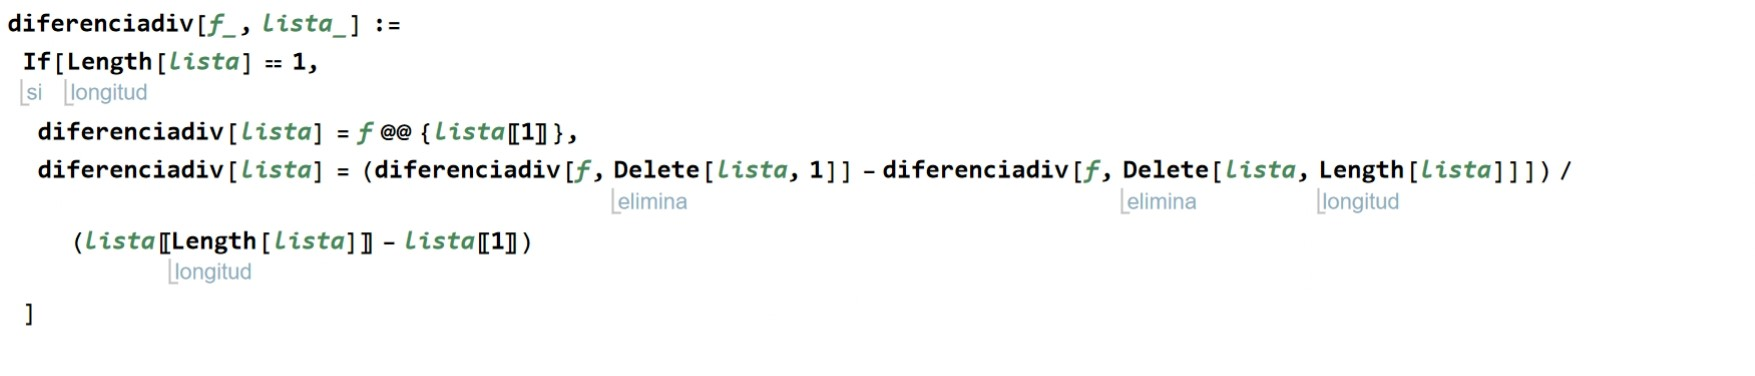
\includegraphics[scale=0.60]{diferencias_divididas.jpg}
        \end{figure}
        
        \noindent \textbf{tabladifdiv[f,$\mathbf{\{x_o,\ldots,x_n\}}$]}: la salida es una tabla con las diferencias divididas $f[x_i,\ldots,x_{j+i}]$ con $i\in\{0,\ldots,n\}$ y $j+i\leq n$
                \begin{figure}[h]
            \centering
            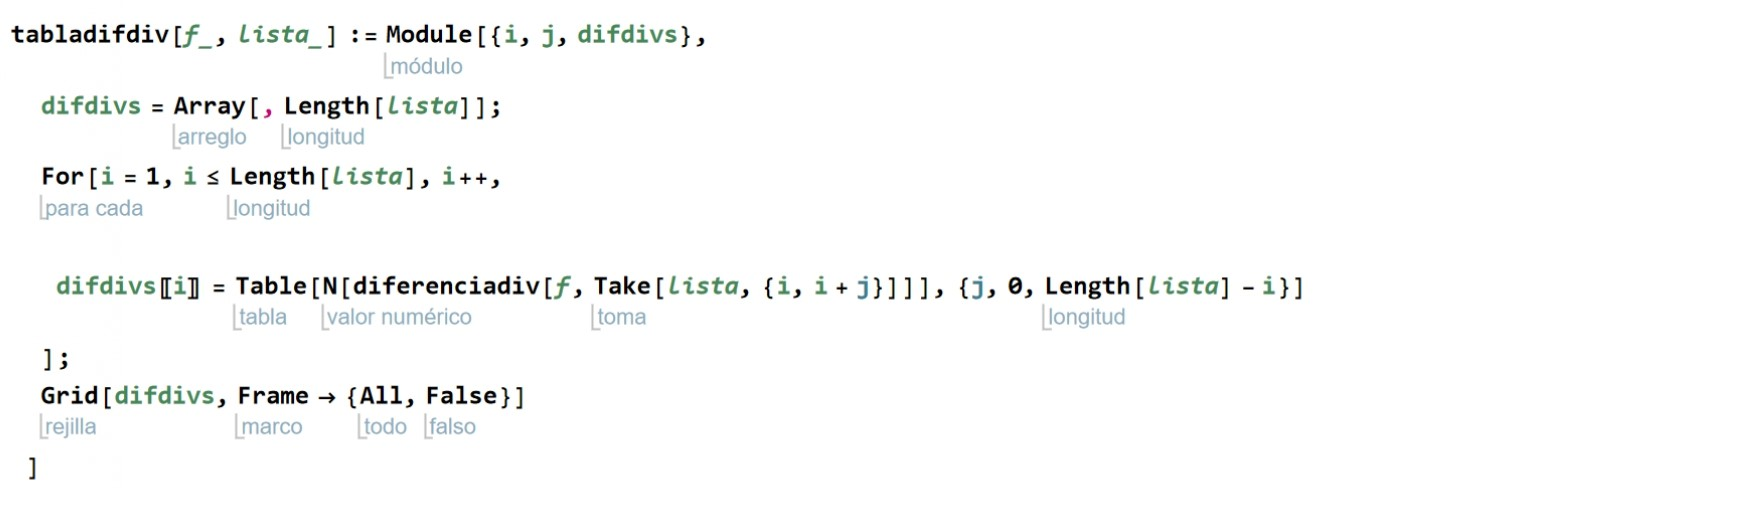
\includegraphics[scale=0.6]{yepa_page-0001.jpg}
        \end{figure}
        
        \noindent \textbf{chebyshev[n]}: calcula el polinomio $T_n(x)$.
          \begin{figure}[h]
            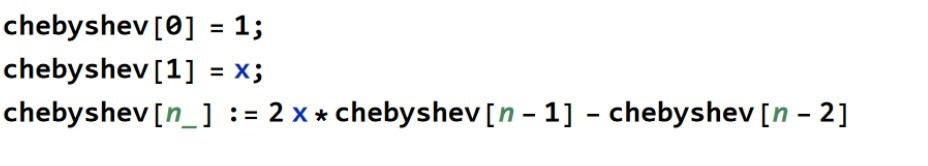
\includegraphics[scale=0.60]{yepa_page-0001 (1).jpg}
        \end{figure}
        
       \noindent \textbf{Plotchebyshev[n]:} si $n\geq 0$ la salida es un gráfico del polinomio $T_n(x)$ y si \newline $n=\{n_1,n_2\}$ la salida es un gráfico de los polinomios $T_{n_1}$ hasta el $T_{n_2}$ .
        
        \begin{figure}[h]  
            \centering
            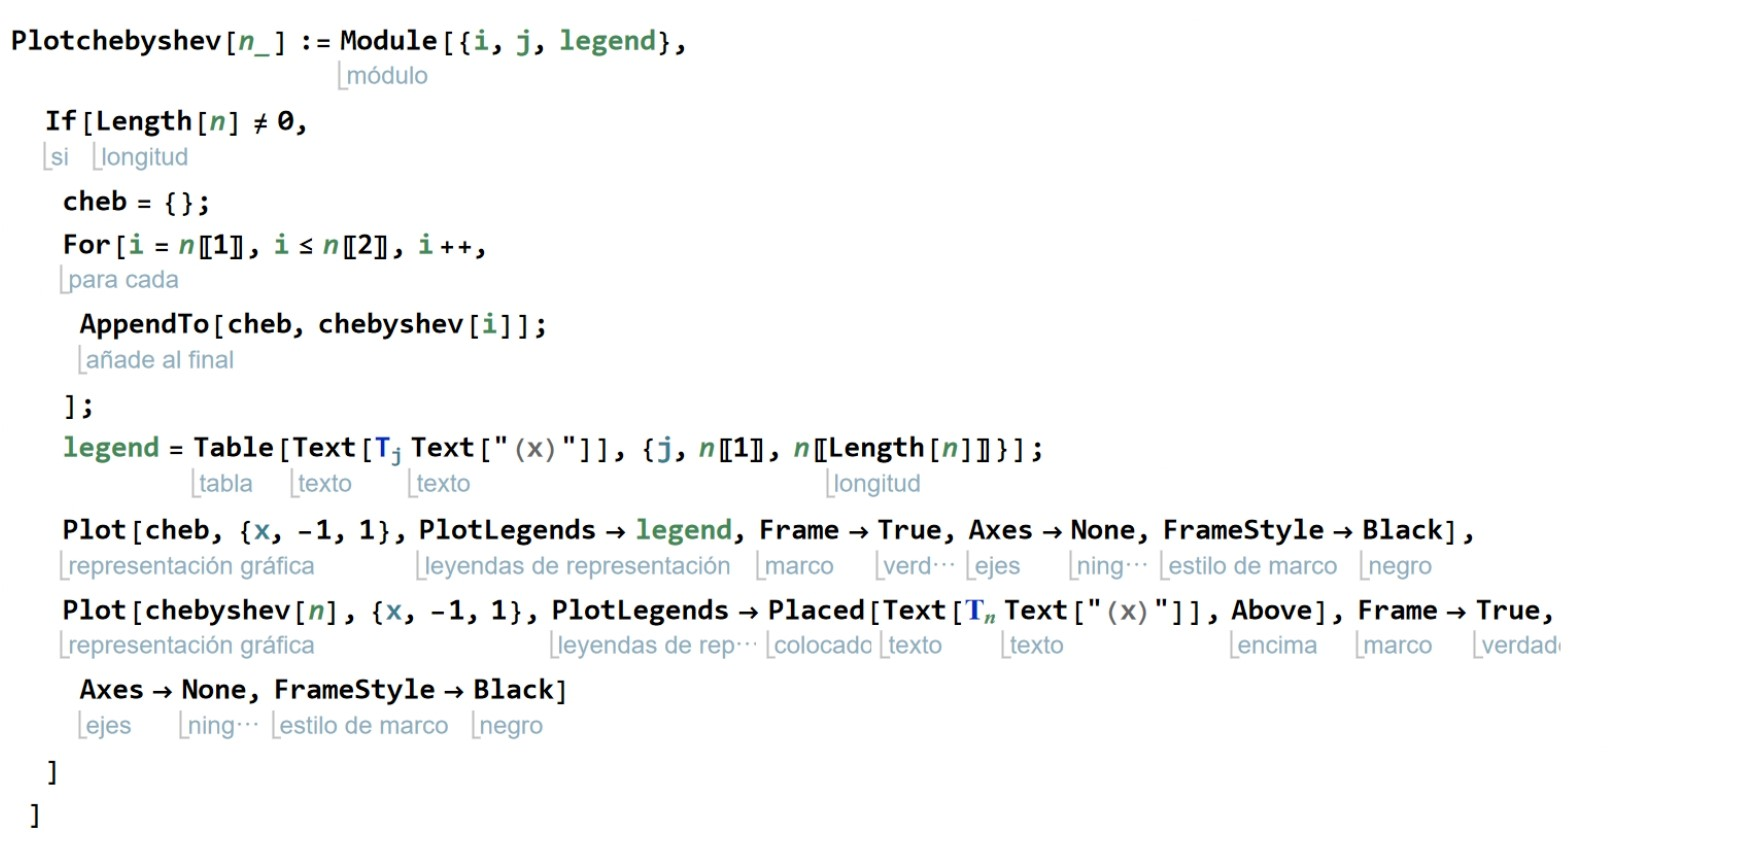
\includegraphics[scale=0.6]{yepa_page-0001 (2).jpg}
        \end{figure}
              \newpage
        \noindent \textbf{Nodoschebyshev[n,\{a,b\}]:} calcula los $n$ primeros nodos de Chebyshev del intervalo $(a,b)$.
        \begin{figure}[h]
            \centering
            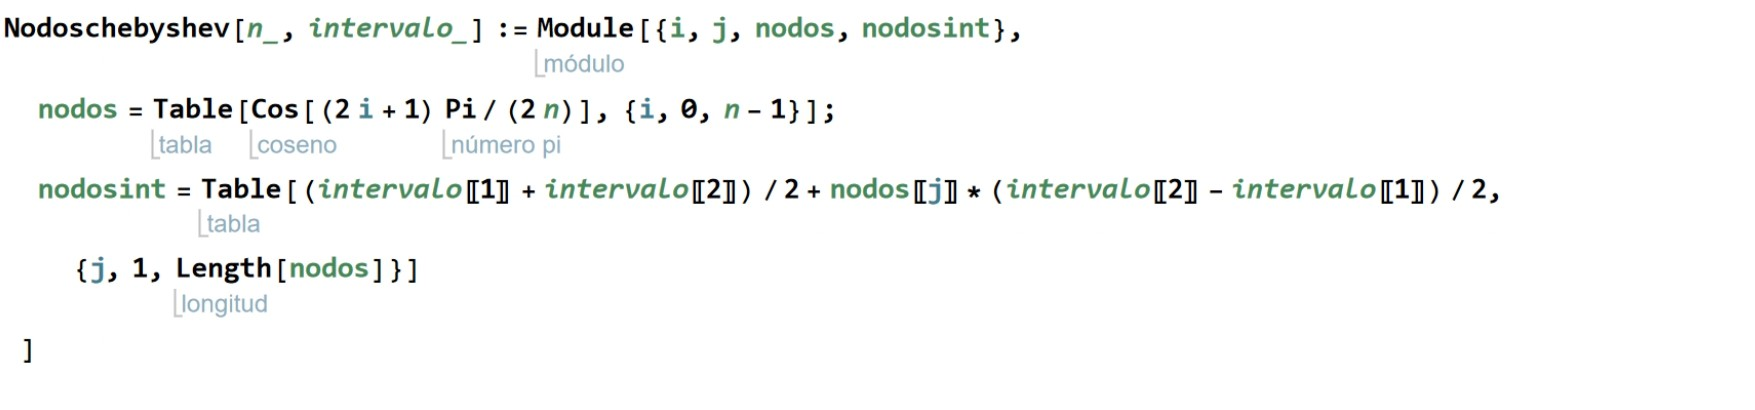
\includegraphics[scale=0.6]{yepa_page-0001 (3).jpg}
        \end{figure}
  
        \noindent \textbf{ChebyshevInt[f,n,\{a,b\}]:} hace un gráfico de la función $f$ junto con el polinomio de interpolación de dicha función en los $n$ primeros nodos de Chebyshev del intervalo $(a,b)$.
        
        \begin{figure}[h]
            \centering
            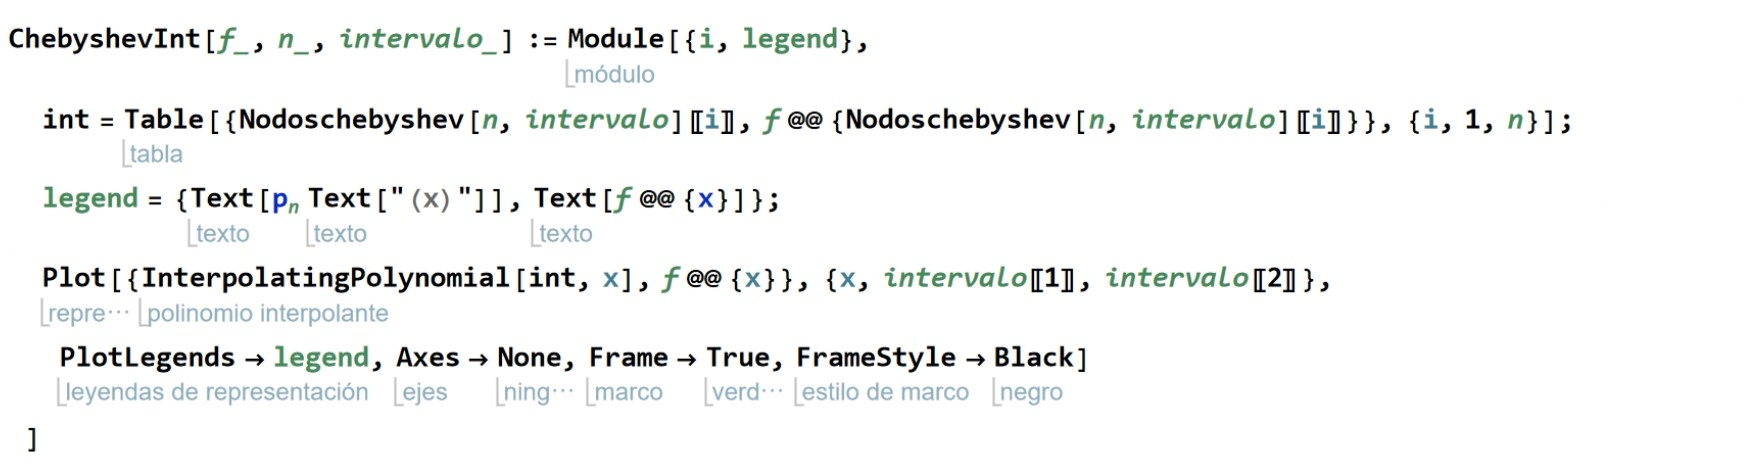
\includegraphics[scale=0.55]{yepa_page-0001 (4).jpg}
        \end{figure}

\end{document}

